% Based on format by Jos� Koiller, Dan Foreman-Mackey

%% Use the first of the following lines during production to
%% easily spot "overfull boxes" in the output. Use the second
%% line for the final version.
% \documentclass[12pt,draft,letterpaper]{report}
\documentclass[12pt,letterpaper]{report}

\newcommand{\thesistitle}{Methods in computational cosmology}
\newcommand{\thesisauthor}{Mohammadjavad Vakili}
\newcommand{\thesisadvisor}{Professor David W. Hogg}
\newcommand{\graddate}{May 2017}

%% The following makes chapters and sections, but not subsections,
%% appear in the TOC (table of contents). Increase to 2 or 3 to
%% make subsections or subsubsections appear, respectively. It seems
%% to be usual to use the "1" setting, however.
\setcounter{tocdepth}{1}

%% Sectional units up to subsubsections are numbered. To number
%% subsections, but not subsubsections, decrease this counter to 2.
\setcounter{secnumdepth}{3}

%% Page layout (customized to letter paper and NYU requirements):
\setlength{\oddsidemargin}{0in}
\setlength{\textwidth}{6.5in}
\setlength{\topmargin}{0in}
\setlength{\headheight}{0in}
\setlength{\headsep}{0in}
\setlength{\textheight}{8.3in}
% \setlength{\footskip}{.5in}
\setlength{\skip\footins}{.3in}

\usepackage{setspace}
% \singlespacing{}
\doublespacing{}

%% This inputs your auxiliary file with \usepackage's and \newcommand's:
%% It is assumed that that file is called "definitions.tex".
\usepackage[final]{graphicx}

\usepackage{color, hyperref}
\definecolor{linkcolor}{rgb}{0,0,0.2}
\hypersetup{colorlinks=true,linkcolor=linkcolor,citecolor=linkcolor,
            filecolor=linkcolor,urlcolor=linkcolor}
\hypersetup{pageanchor=false}

\usepackage{indentfirst}
\usepackage[tbtags]{amsmath}
\usepackage{amsfonts}
\usepackage{amssymb}
\usepackage{booktabs}
\usepackage{url}

% Custom AAS macros:
\usepackage{aas_macros}

% Bibliography:
\usepackage{natbib}
\bibliographystyle{apj}

% Algorithms:
\usepackage{algorithmic,algorithm}

% Commands:

\renewcommand*{\sectionautorefname}{Section} %for \autoref
\renewcommand*{\subsectionautorefname}{Section} %for \autoref
\definecolor{dred}{rgb}{0.75,0.,0.}
\definecolor{darkred}{rgb}{0.5,0.,0.}
\definecolor{darkgreen}{rgb}{0.,0.5,0.}
\definecolor{dred}{rgb}{0.75,0,0}
\definecolor{darkred}{rgb}{0.5,0,0}
\definecolor{darkgreen}{rgb}{0,0.5,0}
\definecolor{darkblue}{rgb}{0,0,0.5}
\hypersetup{ colorlinks,
linkcolor=darkblue,
filecolor=darkgreen,
urlcolor=darkred,
citecolor=darkblue}
\newcommand{\beq}{\begin{equation}}
\newcommand{\eeq}{\end{equation}}
\newcommand{\lang}{\langle}
\newcommand{\ra}{\rangle}
\newcommand{\vep}{\bm{\epsilon}}
\newcommand{\ep}{\epsilon}
\newcommand{\pars}{\vec{\theta}}
\newcommand{\dev}{\mathrm{d}}
\newcommand{\ngal}{n_{g}}
\newcommand{\gmf}{g(N)}
\newcommand{\mr}{M_{\rm r}}
\newcommand{\rpp}{r_{\rm p}}
\newcommand{\mzero}{\log M_{0}}
\newcommand{\mone}{\log M_{1}}
\newcommand{\mmin}{\log M_{\rm min}}
\newcommand{\sigmam}{\sigma_{\log \rm M}} 
\newcommand{\wpp}{w_{\rm p}} 

\newcommand{\acen}{\mathcal{A}_{\rm cen}}
\newcommand{\asat}{\mathcal{A}_{\rm sat}}
\newcommand{\todo}[1]{{\em \textcolor{red}{ #1}}}

\newcommand{\argmax}{\mathrm{argmax}}
\newcommand{\mstar}{h^{-1}M_\odot}



\newcommand{\lcdm}{\Lambda {\rm CDM}}
\newcommand{\mean}[2]{\left\langle#1 \vert {#2}\right\rangle}

%%% HALO OCCUPATION DISTRIBUTION %%%
\newcommand{\nsat}{N_\mathrm{s}}
\newcommand{\ncen}{N_\mathrm{c}}
\newcommand{\pnm}[2]{p(#1|#2)}

\newcommand{\mhalo}{M_{\rm h}}
\newcommand{\mvir}{M_\mathrm{vir}} 

\newcommand{\dndmvir}{\frac{\dd n}{\dd\mvir}}
\newcommand{\dndmhalo}{\frac{\dd n}{\dd\mhalo}}
\newcommand{\dndmvirprime}{\frac{\dd n}{\dd\mvir'}}

%%% CLUSTERING STATISTICS %%%
\newcommand{\xigg}{\xi_{\mathrm{gg}}}
\newcommand{\xihh}{\xi_{\mathrm{hh}}}
\newcommand{\xiggr}{\xi_{\mathrm{gg}}(r)}
\newcommand{\xiggroneh}{\xi^{1h}_{\mathrm{gg}}(r)}
\newcommand{\xiggrtwoh}{\xi^{2h}_{\mathrm{gg}}(r)}
\newcommand{\ngalaxy}{\bar{n}_{\mathrm{g}}}

% General formatting:
\newcommand{\paper}{Chapter}

% Foreign text:
\newcommand{\foreign}[1]{\emph{#1}}
\newcommand{\etal}{\foreign{et\,al.}}
\newcommand{\etc}{\foreign{etc.}}
\newcommand{\eg}{\foreign{eg.}}

% Project references:
\newcommand{\project}[1]{{\textsl{#1}}}
\newcommand{\sdss}{\project{SDSS}}
\newcommand{\boss}{\project{BOSS}}
\newcommand{\hst}{\project{HST}}
\newcommand{\wfc}{\project{WFC3}}

% LaTeX object referencing:
\newcommand{\chapid}{no chapter}
\newcommand{\figref}[1]{\ref{\chapid:fig:#1}}
\newcommand{\Fig}[1]{Figure~\figref{#1}}
\newcommand{\fig}[1]{\Fig{#1}}
\newcommand{\figlabel}[1]{\label{\chapid:fig:#1}}

\newcommand{\Tab}[1]{Table~\ref{\chapid:tab:#1}}
\newcommand{\tab}[1]{\Tab{#1}}
\newcommand{\tablabel}[1]{\label{\chapid:tab:#1}}

\renewcommand{\eqref}[1]{\ref{\chapid:eq:#1}}
\newcommand{\Eq}[1]{Equation~(\eqref{#1})}
\newcommand{\eq}[1]{\Eq{#1}}
\newcommand{\eqalt}[1]{Equation~\eqref{#1}}
\newcommand{\eqlabel}[1]{\label{\chapid:eq:#1}}

\newcommand{\sectionname}{Section}
\newcommand{\sectref}[1]{\ref{\chapid:sect:#1}}
\newcommand{\Sect}[1]{\sectionname~\sectref{#1}}
\newcommand{\sect}[1]{\Sect{#1}}
\newcommand{\sectalt}[1]{\sectref{#1}}
\newcommand{\App}[1]{Appendix~\sectref{#1}}
\newcommand{\app}[1]{\App{#1}}
\newcommand{\sectlabel}[1]{\label{\chapid:sect:#1}}

\newcommand{\Algo}[1]{Algorithm~\ref{\chapid:algo:#1}}
\newcommand{\algo}[1]{\Algo{#1}}
\newcommand{\algolabel}[1]{\label{\chapid:algo:#1}}

\newcommand{\chapname}{Chapter}
\newcommand{\Chap}[1]{\chapname~\ref{chap:#1}}
\newcommand{\chap}[1]{\Chap{#1}}
\newcommand{\chapalt}[1]{\ref{chap:#1}}
\newcommand{\chaplabel}[1]{\label{chap:#1}}

\newcommand{\dfmtodo}[1]{\todo{DFM}{red}{#1}}

% Math:
\newcommand{\dd}{\ensuremath{\,\mathrm{d}}}
\newcommand{\bvec}[1]{{\ensuremath{\boldsymbol{#1}}}}
\newcommand{\paramvector}[1]{\bvec{#1}}
\newcommand{\unit}[1]{\mathrm{#1}}

% Probabilities:
\newcommand{\like}{\mathscr{L}}
\newcommand{\pr}[1]{\ensuremath{p(#1)}}
\newcommand{\af}{\ensuremath{a_f}}
\newcommand{\expect}[1]{\left<#1\right>}
\newcommand{\normal}[2]{\mathcal{N} (#1, #2)}

\sloppy\sloppypar


\begin{document}

%% Produces a test "layout" page, for "debugging" purposes only.
%% Comment out for final version.
% \layout  % requires package layout (see above, on this same file)

%%%%%% Title page %%%%%%%%%%%
%% Sets page numbering to "roman style" i, ii, iii, iv, etc:
\pagenumbering{roman}
%
%% No numbering in the title page:
\thispagestyle{empty}
%
\begin{center}


    \vspace*{0.5in}
    {\large\textbf{\thesistitle}}
    \vspace{.4in}

    by
    \vspace{.4in}

    \thesisauthor{}
    \vspace{.8in}
    % \vfill

    \begin{doublespace}
        A dissertation submitted in partial fulfillment \\
        of the requirements for the degree of \\
        Doctor of Philosophy \\
        Department of Physics \\
        New York University \\
        \graddate{}
    \end{doublespace}
\end{center}
\vfill

\noindent\makebox[\textwidth]{\hfill\makebox[2.5in]{\hrulefill}}\\
\makebox[\textwidth]{\hfill\makebox[2.5in]{\hfill\thesisadvisor\hfill}}
\newpage

% %%%%%%%%%%%%%% Copyright %%%%%%%%%%%%%%%%%
\vspace*{\fill}
\begin{center}
    Copyright \textcopyright\ 2017 Mohammadjavad Vakili \\
    This work is licensed under a Creative Commons Attribution 4.0
    International License.
    \addcontentsline{toc}{section}{Copyright}
\end{center}
\vfill
\newpage

%%%%%%%%%%%%% Blank page %%%%%%%%%%%%%%%%%%
\thispagestyle{empty}
\vspace*{0in}
\newpage

%%%%%%%%%%%%%% Acknowledgements %%%%%%%%%%%%
%% Comment out the following lines if you do not want to acknowledge
%% anyone's help...
\section*{Acknowledgements}\addcontentsline{toc}{section}{Acknowledgements}
I am grateful to David Hogg for being a great advisor and teacher. 
I thank him for his consistent support, encouragement, patience, teachings, 
and all the valuable skills I learned from him.

I thank David Hogg, Jeremy tinker, Michael Blanton, and Boris Leistedt for reading an initial draft of 
thesis and sharing their valuable comments with me.

Throughout my PhD years, I have had the opportunity to immensly benefit from collaboration and 
interaction with Ross Fadely (Insight), ChangHoon Hahn (NYU), Andrew Hearin (Yale), Dan Foreman-Mackey (UW), 
Kilian Walsh (NYU), Paco Kitauro (IAC), Yu Feng (Berkeley), Albert Chuang (Leibnitz), and Alex Malz (NYU).

I would like to acknowledge the fantastic computational support that I received at NYU. 
I am grateful to Shenglong Wang (the administrator of NYU HPC) and Mulin Ding (the administrator 
of CCPP computational facilities) for their persistent support and phenomenal work ethics. 

%I would also like to thank David Hogg, Dan Foreman-Mackey, Dustin Lang, Jeremy Tinker, and Gustavo Yepes for their computational support. 

I truely enjoyed the lively and intellectually stimulating atmosphere at CCPP.
I also want to thank all my great friends in graduate school who helped create a 
supportive and joyful environment.  

I also thank my family who have always supported me throughout my entire life.



\newpage

%%%% Abstract %%%%%%%%%%%%%%%%%%
\section*{Abstract}\addcontentsline{toc}{section}{Abstract}
State of the inhomogeneous universe and its geometry throughout cosmic history can be studied by measuring the clustering of galaxies and the gravitational lensing of distant faint galaxies. Lensing and clustering measurements from large datasets provided by modern galaxy surveys will forever shape our understanding of the how the universe expands and how the structures grow. Interpretation of these rich datasets requires careful characterization of uncertainties at different stages of data analysis: estimation of the signal, estimation of the signal uncertainties, model predictions, and connecting the model to the signal through probabilistic means. In this thesis, we attempt to address some aspects of these challenges.  

The first step in cosmological weak lensing analyses is accurate estimation of the distortion of the the light profiles of galaxies by large scale structure. These small distortions, known as the cosmic shear signal, are dominated by extra distortions due to telescope optics and atmosphere (in the case of ground-based imaging). This effect is captured by a kernel known as the Point Spread Function (PSF) that needs to be fully estimated and corrected for. We address two challenges a head of accurate PSF modeling for weak lensing studies. The first challenge is finding the centers of point sources that are used for empirical estimation of the PSF. We show that the approximate methods for centroiding stars in wide surveys are able to optimally saturate the information content that is retrievable from astronomical images in the presence of noise. 

Furthermore, we demonstrate how we can infer the PSF from the poorly sampled images taken with detectors of the space-based telescopes such as the Hubble Space Telescope (HST). 
Weak lensing studies of galaxies that are poorly resolved by these telescopes requires knowledge of the PSF at a resolution higher than the pixel resolution of HST. 
In particular, we present a forward model of the point sources as observed by the HST WFC3 IR channel. We show that this forward model can accurately estimate the super-resolution PSF. We also introduce a noise model that permits us to robustly analyze the HST WFC3 IR observations of the crowded fields.    

Then we try to address one of the theoretical uncertainties in modeling of galaxy clustering on small scales which requires assuming a halo model. Clustering of halos has been shown to depend on halo properties beyond mass such as halo concentration, a phenomenon referred to as assembly bias. Standard large-scale structure studies with halo occupation distribution (HOD) assume that halo mass alone is sufficient in characterizing the connection between galaxies and halos. However, assembly bias could cause the modeling of galaxy clustering to face systematic effects if the expected number of galaxies in halos is correlated with other halo properties. Using high resolution N-body simulations and the clustering measurements of Sloan Digital Sky Survey DR7 main galaxy sample, we present the extent to which the dependence of galaxy clustering modeling on halo properties beyond mass can improve our modeling of galaxy clustering.

One of the key ingredients in precise parameter inference using galaxy clustering is accurate estimation of the error covariance matrix of clustering measurements. This requires generation of many independent galaxy mock catalogs that accurately describe the statistical distribution of galaxies in a wide range of physical scales. We present a fast and accurate method based on low-resolution N-body simulations and an an empirical bias model for for generating mock catalogs. We use fast particle mesh gravity solvers for generation of dark matter density field and we use MCMC to estimate the bias model that connects dark matter to galaxies. We show that this approach enables of to generate mock catalogs that recover clustering at a percent-level accuracy down to quasi-nonlinear scales. 

Cosmological datasets are interpreted by specifying a likelihood function that is often assumed to be multivariate Gaussian. Likelihood free approaches such as Approximate Bayesian Computation (ABC) can bypass this assumption by introducing a generative forward model of the data and a distance metric for quantifying the closeness of the data and the model. We present the first application of ABC in large scale structure for constraining the connections between galaxies and dark matter halos. We show that ABC equipped with Population Monte Carlo and a generative forward model of the data that incorporates sample variance and systematic uncertainties can accurately estimate the parameters given the galaxy clustering and galaxy group statistics measurements.  

\newpage

%%%% Table of Contents %%%%%%%%%%%%
\tableofcontents

%%%%% List of Figures %%%%%%%%%%%%%
%% Comment out the following two lines if your thesis does not
%% contain any figures. The list of figures contains only
%% those figures included withing the "figure" environment.
\newpage\addcontentsline{toc}{section}{List of Figures}
\listoffigures

%%%%% List of Tables %%%%%%%%%%%%%
%% Comment out the following two lines if your thesis does not
%% contain any tables. The list of tables contains only
%% those tables included withing the "table" environment.
\newpage\addcontentsline{toc}{section}{List of Tables}
\listoftables
\newpage

%%%%% Body of thesis starts %%%%%%%%%%%%
\pagenumbering{arabic}

%% Introduction. If your thesis has no introduction, or chapter 1 is
%% meant to be the introduction, then comment out the lines below.
\chapter*{Introduction}\addcontentsline{toc}{chapter}{Introduction}

Cosmology is entering a new era. Thanks to the ongoing and 
the upcoming low redshift galaxy surveys as well as the early universe probes, 
we are able to put cosmological theories into test with high precision.
With the observations of the cosmic microwave background (CMB) radiation 
and the distant Type Ia supernovae, our understanding of universe was 
revolutionized in the late 90s. Later datasets advanced our understanding 
of the universe even further.

The early universe was in a hot and dense state where 
matter and radiation formed a primordial plasma. Eventually, the 
plasma cooled down, first atoms formed and photons started streaming freely.  
Today, we can observe these ancient photons as a microwave background radiation. 
The temperature of this radiation is approximately $2.7 \; K$ in all directions with 
fluctuations that are 1 part in 10000.

In a strikingly great agreement with the CMB observations, models of inflation---nearly 
exponential rapid phase in the expansion of early universe--- 
predict \emph{nearly Gaussian and scale invariant} random fluctuations around a homogeneous 
background. Microscopic quantum fluctuations generated in an inflationary 
stage were stretched to cosmic volumes. Evolution of these initial seeds 
resulted in the formation of structures such as planets, stars, galaxies, 
clusters of galaxies, filaments, \emph{etc}.

By measuring the brightness of supernovae type Ia, we have also learned 
that supernovae Ia are fainter than what we expect them to be in an 
expanding universe filled with matter. This surprising observation led us to 
believe that approximately 70 $\%$ of the energy budget of the universe is 
given by a dark energy component which can be considered a liquid with 
negative pressure.

From a theoretical standpoint, cosmic acceleration 
can be explained in numerous modified gravity frameworks. 
Despite the astonishing success of general relativity in 
certain regimes such as the solar system, binary pulsars, 
and gravitational waves as a result of merging supermassive blackholes, 
precision test of GR on large scales remains an active area of research. 
Current constraints on the accelerated expansion and growth of structure 
can not rule out with certainty some of the theories of modified gravity.

Detection of the Baryonic Acoustic Oscillation feature in clustering of galaxies 
further enhanced our understanding of the expansion history. 
Acoustic oscillations in the early universe plasma result in a sound wave 
that leaves an imprint with a characteristic scale on the perturbations 
in late time universe. Therefore the BAO provides a highly accurate estimate of the angular diameter 
distance and it provides a powerful probe of the geometry and expansion history of the universe. 

In galaxy redshift surveys, the distances to galaxies can be estimated by the measured 
redshifts. The distance information provided by these surveys is distorted by the peculiar 
velocities of galaxies along the line of sight. These distortions are referred to as redshift space 
distortions (RSD). Redshift space distortions are highly sensitive probes of the growth of structure 
and contain additional cosmological information beyond what is provided by the BAO feature. 
Thus measurements of galaxy clustering with redshift surveys can 
constrain dark energy and laws of gravity.

%Spectroscopic surveys such as eBOSS \citep{eboss}, DESI, and Euclid \citep{euclid} allow us to precisely 
%constrain the expansion history of the universe as well as the growth of structure. 
%However, interpretation of these rich datasets requires characterization of the uncertainties on the clustering 
%measurements of these datasets. The uncertainties are estimated in terms of the covariance matrix. Precision matrix, 
%the inverse of the covariance matrix appears in the cosmological likelihood 
%(the probability of the observed data given the model).

%These constraints will enable us to distinguish between different physical scenarios that explain the accelerated expansion of the universe. 
%A crucial component of BAO and RSD analyses is estimation of the uncertainties of the statistical summaries of 
%the data obtained from galaxy surveys. One of the most promising frameworks for estimating the uncertainties in form of covariance matrices is production 
%of a large number of accurate simulations of our observations. 

The large datasets from galaxy surveys are analyzed by estimating the statistical summaries of the 
data and then interpreting them with the predictions from cosmological theories. This is formally done 
by writing down a likelihood function which is the probability of the observed data given the theoretical model under 
consideration. Cosmological likelihood functions are often assumed to have a Gaussian 
functional form. Given this assumption, the likelihood can be fully specified with three ingredients: a data vector which is estimated from observations, a mean model vector 
which is computed from the predictions of theoretical models, and an inverse covariance matrix. 

Therefore, a crucial step in interpreting the data is computing the error covariance matrix. 
In fact, the quantity that we need to know precisely is the inverse covariance matrix (precision matrix) because it is this matrix that appears in the likelihood function. Modern cosmological analyses rely on computing the covariance matrix analytically, estimating the matrix from a large suite of simulations, or from internal resampling of the data. 

Motivated by the pursuit of minimizing the effect of the noise properties of the precision matrix on 
cosmological parameter estimation, \citet{dodelson2013,taylor2013,taylor2014} derived a set of requirements 
on the number of independent mock simulations given the number of data points and the number of parameters 
in a given cosmological analysis. Assuming that the estimated covariance matrix follows a \emph{Wishart} distribution, 
\citep{Sellentin:2016a} present a method for marginalizing over the precision matrix. They demonstrate that the 
resulting likelihood function is no longer Gaussian and instead follows a $t$-distribution.

\citet{dodelson2013,Sellentin:2017a} demonstrate that a noisy estimate of the precision matrix 
constructed from insufficient number of simulated mocks can systematically bias the confidence 
intervals over the cosmological parameters. These findings place strict requirement on the number of 
mock catalogs for the ongoing and future galaxy surveys. In general, the number of mocks need to be much larger than 
the number of data points.

Common practices in analysis of deep imaging surveys are tomographic binning of the data and combining probes.
In tomographic binning, the dataset is split into multiple redshift slices and the summary statistics of 
the data are estimated by correlating the data within each redshift slice and cross-correlating the data across 
multiple redshift slices. The size of the resulting data vector can be as large as a few hundred which makes the task of creating mock catalogs even more challenging. 

Combining probes involves joint analysis of different cosmic probes such as galaxy 
positions and galaxy shears. Multi-probe analyses are more robust against systematic 
uncertainties (specially systematics that only affect one of the probes) 
and have more constraining power. Most modern surveys offer this great opportunity. 
One of the main obstacles a head of these efforts is the large data vector under investigation. 
Production of the covariance of this data vector requires many simulations which may not 
be feasible to provide.   

Analytical covariance matrices on the other hand, are not as computationally demanding. 
Their inverse (precision matrix) is noise free. But the model approximations and assumptions used in these methods may not be sufficient for the accuracy requirements of precision cosmology. Analytical covariance matrices are considered to receive Gaussian and a non-Gaussian contributions. Assuming that the density field is a 
Gaussian random field, the Gaussian part of the covariance matrix is straightforward to compute \citep{grieb2016,klaus2016,slepian2016b}.

Including the non-Gaussian part of the covariance matrix however, is necessary for accurate parameter estimation \citep{takahashi2011,blot2016,chan2016}.
Significant progress has been made in modeling the non-Gaussian contribution to covariance matrices based on perturbation theory and effective theories of large scale structure \citep{mohammed_seljak,mohammed2017} or by adopting halo (virialized regions of matter overdensity) model \citep{takada_spergel,eifler2014}.
Regardless of the applicability of analytical covariance matrices in analyzing the survey data, production of simulated mocks remains an important step in \emph{validation} and \emph{calibration} of these analytical covariance matrices \citep{slepian2016b,hildebrandt2017}.

Considerable progress has been made in developing methods that take into account our prior beliefs 
about the of covariance matrices. By considering sparsity of the covariance matrix, \citet{paz2015,padmanabhan2016} 
present methods to estimate the precision matrices with fewer mocks. Shrinkage methods \citep{pope2008,joachimi2016} 
also require fewer simulations. \citet{fried2017} presents a trick for expanding the precision matrix 
around a part that can be easily computed through analytical means and estimating the leading expansion terms with finite number of simulations.

One of the common tools for estimation of covariance matrices is internal resampling of the data such as jackknife and bootstrap. These estimators have been extensively used in analyses of galaxy clustering and galaxy-galaxy lensing (for example see \citealt{reid2014,hod_vs_sham,shirasaki2016,singh2016,kwan2017}).
In certain cases when no reliable analytical or simulation-based estimate of the covariance is available, one could use these estimators. 
For instance in Chapter 3, for interpreting the SDSS DR7 galaxy clustering measurements, 
we make use of covariance estimates based on jackknife resampling of the data. But as \citet{norberg,fried2016} point out, data resampling methods do not faithfully capture the uncertainties of the data. 

Precision estimation of the covariance matrix from mocks requires generation of a large number of mocks for a given analysis. This has led to development of \emph{approximate} \emph{methods} for mass production of galaxy and halo mock catalogs. Approximate methods rely on approximate gravity solvers for generating dark matter density fields with reasonable accuracy on large scales and statistical prescriptions for populating the dark matter density field with mock galaxies (see for example \citealt{pthalo,qpm,eazymock,kitaura2016} and references 
therein). The state-of-the-art techniques for production of mock catalogs are QPM \citep{qpm} and PATCHY \citep{kitaura2016}. These methods were used in 
cosmological analyses of the SDSS III-BOSS final data release \citep{alam2016}.

In the PATCHY method the density field is generated with perturbation theory. Then the expected number of galaxies in a cosmic volume given the density field is computed according to a biasing relation whose parameters are unknown. 
Finally, the number of galaxies is drawn from a negative binomial distribution which is a Poisson distribution with additional stochasticity. 
\citet{chuang2015} demonstrates that this approach is very powerful at reproducing the two-point and three-point statistics of galaxies with high accuracy toward mildly nonlinear regimes.

In Chapter 4, we address two limitations of this method: \emph{bias} \emph{estimation} and \emph{accuracy on small scales}. We replace the perturbation theory-based 
gravity solver of the PATCHY code with the fast particle mesh (PM) method of \citet{fastpm}. The main difference between the Particle mesh implementations of \citet{fastpm} and \citet{qpm} is that 
FastPM imposes exact large scale growth and thus it does not suffer from the loss of power on large scales as a result of using a limited number of time steps for solving equations of motion. We also introduce an automatic bias estimation method based on MCMC. 

In comparison with the previous version of the code based on perturbation theory, our novel approach yields higher accuracy toward nonlinear scales for both two-point 
and three-point statistics. One of the main advantages of our approach is the following. In order to reach reasonable accuracy, the common approximate $N$-body methods \citep{qpm,fastpm,ice_cola} require a larger grid size than the number of particles. That is, the gravitational forces between the particles need to be calculated on a mesh (at least) twice larger than the number of particles (see also \citealt{chuang2015,monaco2016}) in order to resolve halos. We note that our effective bias prescription for populating the dark matter density field with halos bypasses this requirement and as a consequence, it significantly reduces the computational cost of generating mocks.      
%%%%%%%%%%%%%%%%%%%%%%%%%%%%%%%%%%%%%%%%%%%%%%%%%%%%%%%%%%%%%%%%%%%%%%%%%%%%%%%%%%%%%%%%%%%
Gravitational lensing of luminous sources (galaxies, CMB) can measure 
the state of the inhomogeneous matter density and the time-dependence of dark energy. 
Lensing of the light emitted by background faint galaxies by the intervening large scale structure 
results in very small but correlated distortions in the shapes of galaxies. This phenomenon is referred to 
as cosmic shear.

Cosmic shear studies are hurdled by a number of statistical uncertainties (unknown distribution 
of galaxy intrinsic morphologies) and systematics. The long list of systematic error budget 
of cosmic shear studies can in general fall into the following categories: uncertain distance 
(photometric redshift) information, and imperfect knowledge of intrinsic alignments of galaxies and non-linear matter 
power spectrum models, and image systematics. 

Tomographic reconstruction of the distribution of dark matter with imaging surveys requires 
accurate distance information which is encoded in the redshifts of galaxies. 
The redshift that are estimated from the imaging surveys are usually uncertain as they are measured with coarse 
spectra in the form of a few magnitude numbers based on broadband photometry. These redshifts are called 
photometric redshifts and their accuracy depends on the number of broadband filters and the overlapping spectroscopic 
sample of galaxies \citep{bonnett2016,choi2016,boris2016,hildebrandt2017}. %FIXME BORIS AND HOGG?

Intrinsic alignment of galaxies (IAs) also contaminate the cosmic shear signal. These IAs, if not accounted for, 
can significantly bias the cosmological parameter inference \citep{codis2015,joachimi2015, kirk2015,krause_ia}. 
Cosmological interpretation of the cosmic shear signal requires an accurate knowledge of the nonlinear 
matter power spectrum \citep{semboloni2013, eifler2015, schaye2015, joudaki2016, kitching2016, mead2016}. Modeling the role of 
Baryonic feedback and the accuracy of the emulators for nonlinear matter clustering remains an active area of research. 

Perhaps the most widely and extensively studied sources of systematics in weak lensing are the image systematics which make 
the process of inferring the cosmic shear from noisy images of galaxies far from trivial. The light profile of 
galaxies is distorted with the atmosphere and telescope optics. The amount of distortion is captured in a kernel called 
the Point Spread Function (PSF). The size and shear of the background galaxies used in weak lensing studies is often 
smaller than those of the PSF, making the cosmic shear signal dominated by the PSF which is empirically estimated at 
the positions of stars and then interpolated to the positions of galaxies.  

Furthermore, additional systematics arise from unrealistic models of galaxy light profile \citep{voight2010,im3shape,kac2014}, 
detector effects \citep{arun2016,jaya2016,plazas2016}, nonlinear dependence of galaxy ellipticities 
on the pixel data in the presence of noise that biases the shear \emph{point} \emph{estimates} \citep{melchoir,great3,conti2017}, 
and incorrect model of the PSF or inaccurate PSF interpolation \citep{rowe2010,kuijken2015,great3,des}.

These systematics lead to shear calibration biases in the form of additive and multiplicative 
shear biases. For instance, an incorrect size or anisotropy in the PSF model can introduce 
a multiplicative bias shear. This bias gives rise to a spurious correlation function with the 
same order of magnitude as the cosmological signal.

The shear biases are either calibrated with realistic image simulations \citep{im3shape,jee2016,conti2017} or through cross correlation of 
the cosmic shear signal with other cosmic probes that do not suffer from the same biases (\eg\ galaxy positions)
\citep{liu2016,schann,singh2017}. 

Simulation based techniques are limited due to difficulty in 
generation of realistic galaxy image simulations \citep{great3,lanus2017} and our limited ability to match the depth and detection limits of 
the imaging surveys \citep{hoekstra}. The limitation of cross-correlation technique is that it makes strong assumptions about the assigning a 
single bias parameter to a large population of galaxies under consideration. The shear biases have been shown to be scale-dependent \citep{des,jee2016} 
and depend on morphological properties of galaxies \citep{im3shape,conti2017}. 

Novel shear inference models that do not rely on delivering a point-estimate for the shear signal \citep{schneider,bernstein,huff,sheldon} 
provide promising venues for mitigation of biases but their accuracy is limited to the accuracy in the PSF model.
In chapters 1 and 5, we try to address two challenges in accurate PSF modeling that could lead to biases in cosmological weak lensing analysis. 

One of the steps of astronomical image processing that could lead to inaccurate model of the PSF is centroiding 
of stars. An erroneous method for determination of the centroid of stars could lead to both inaccurate estimation of the 
PSF at the positions of stars and inaccurate PSF interpolation \citep{anderson2000,sdss,anderson2003,desc}. Large astronomical surveys rely on approximate 
methods for centroiding the stars \citep{sextractor,sdss,des}. 

In chapter one we argue that in the presence of noise, there exist
a lower bound on the error arising from centroiding methods. We show that this theoretically set lower bound, also known as the Cram\'{e}r-Rao lower bound \citep{lecam}, 
is \emph{almost} saturated by centroiding methods that rely on correlating the images of stars with the PSF or some approximation to the 
PSF. These centroiding methods are called matched-filter centroiding methods and in certain limits provide an approximation to the more accurate 
methods that rely on fitting a model to the stars. In other words, the Cram\'{e}r-Rao bound provides the minimum achievable information loss by an estimator and 
we show that under certain circumstances, matched-filter centroiding methods achieve this goal.

Additionally, weak lensing shear couples the short wavelength and long wavelength modes of the galaxy light profiles. 
Therefore estimation of the response of galaxy light profile to shear requires knowing the model of galaxy image 
with a resolution better than the PSF that the image of galaxy is convolved with. 

In most space-based telescopes \citep{euclid,wfirst}, the detectors are designed to be large in order to yield wider field of view. 
That is, the detectors sample the light profile of the PSF at a low resolution. In such cases, a large fraction of the light of a given point source 
is captured by the pixel that contains the centroid of the point source. In other words, the PSF is \emph{undersampled}.

Most galaxies of interest for weak lensing studies with these space-based weak lensing experiments are unresolved. 
As a consequence, estimating the shear from unresolved galaxy images requires 
knowing the the galaxy light profile model and the PSF at higher resolutions than the native pixel size of these telescopes \citep{olic,ngole2}.

The filters in HST WFC3 IR channel have the most undersampled detectors among all HST filters. 
As such, HST WFC3 IR channel could benefit a lot from an accurate model of its super resolution PSF. 
In this chapter 5, we present the first generative forward model of stellar sources as observed by the HST camera.
Unlike previous attempts at inferring the PSF model of HST WFC3, our model is data driven in that it makes 
use of the observed data and it presents a proper treatment of modeling in the presence of damaged pixels and overlapping 
point sources.  

Galaxies are luminous tracers of the large scale structure. Thus study of galaxy clustering o understand the growth of structure is 
one of the key drivers of low redshift surveys. Significant progress has been made in linking the observations of 
galaxies and our theoretical understanding of the nonlinear evolution of dark matter. 

On large scales, cosmological perturbation theory equipped with a prescription for galaxy bias permits us 
to accurately model the clustering of galaxies. However, nonlinear evolution of matter 
poses a challenge to applicability of perturbative approaches in small scales. In such limits, 
galaxy clustering must be understood within the context of the halo model which has had 
much success in describing time evolution of the clustering of matter.  

Modeling galaxy clustering with the halo model follows two central assumptions. \emph{First}, galaxies form in virialized regions of 
dark matter overdensity known as halos. \emph{Second}, clustering of galaxies is governed by clustering of dark matter halos. 
In order to use galaxy clustering measurements for gaining insight into cosmological structure formation models we need to 
know how clustering of galaxies can be determined from clustering of halos. That is, we are required to specify how halos 
are populated with galaxies \citep{seljak2000,scoccimarro2001,berlind_weinberg2002}.

One of the successful prescriptions for assignment of galaxies to halos is the halo occupation distribution (HOD). 
HOD provides a prescription for the expected number of galaxies that reside a halo as well as 
the positions and velocities of galaxies that are distributed within a halo. It usually assumes that the halo mass alone 
is sufficient halo property for characterization of this prescription. This simple assumption has been useful 
in reproducing the observed statistics of galaxies \citep{tinker_rsd2007,zehavi2011,zheng_guo}.

Despite being successful at reproducing a wide range of the spatial statistics of galaxies, the simple \emph{mass-only} HOD 
remains challenged by a theoretical phenomenon known as assembly bias. Assembly bias, seen in $N-$body simulations, states that at a fixed halo mass, clustering 
of halos depend on halo properties beyond mass such as their formation history, gravitational potential, \etc\ \citep{weschler2006,gao2007,arz2014,sunayama2016}.
This theoretical prediction has not yet been confirmed with observations and there are very mixed results in the literature.

By weak lensing analysis of the galaxy groups in GAMA (GAlaxy and Mass Assembly, see \citealt{driver}) 
with the KiDS (Kilo Degree Survey, see \citealt{kuijken2015}) imaging data, \citet{dvornik2017} find no evidence for halo assembly bias.
Using the galaxy-galaxy lensing and clustering measurements of SDSS galaxy \emph{redmapper} clusters \citep{rykoff} with halo masses $10^{14}$ $M_{\odot}$, 
\citet{miyatake2016} claimed strong difference between the bias of two populations of clusters with different radial distribution of satellite galaxies 
(a proxy for the formation history of a dark matter halo). \citet{zuetal2016} argues that the findings of \citet{miyatake2016} is most likely due to projection effects (as a result of highly uncertain photometric redshifts) and they cannot be interpreted as detection of assembly bias. 

The effect of assembly bias on galaxy clustering can be seen in many subhalo abundance matching (SHAM, see \citealt{hearin2014,lehman2015} and references therein) methods. SHAM assumes a one-to-one relation between halo (including subhalos) properties (\eg\ mass, circular velocity) and some galaxy properties (\eg\ stellar mass, luminosity). In Chapter 3, with the clustering measurements of SDSS DR7 main sample of galaxies \citep{abazajian2009} and the Small MultiDark $N$-body simulation, we show that the clustering predictions of \citep{decorated} HOD model that takes assembly bias into account are consistent with the predictions of the \emph{mass-only} HOD model within 1-$\sigma$ level. 

We also note that for the sample of $L_{\star}$ galaxies, there is \emph{slight} improvements in galaxy clustering predictions of the HOD model with assembly bias 
on large scales. Furthermore, we note that in terms of information criteria, there is no gain in using a more complex HOD model to fit the clustering measurements.
We note that in terms of the impact of halo assembly bias on galaxy clustering, our constraints show qualitatively similar behavior to the predictions of subhalo abundance matching models. Unlike the findings of \citet{zentner2016}, we do not find any evidence for assembly bias in the satellite population of galaxies.

One of the perplexities faced by contemporary cosmology is the discordance between the constraints on cosmological parameters from some of the low redshift probes and 
the Planck CMB results \citep{planckII}. This includes the cosmological constraints from the cosmic shear analysis of CFHTLenS \citep{heymans,kitching2016} and KiDs \citep{hildebrandt2017}. The disagreement appears in the constraints over the parameters $\sigma_{8}$ (the amplitude of the linear matter power spectrum) and $\Omega_{m}$ (the amount of matter). This tension exists at a 2-$\sigma$ level. 

This \emph{cosmic} \emph{discordance} persists even when the low redshift probe under consideration is galaxy-galaxy lensing which contains information regarding galaxy-matter cross correlation. Similar to galaxy clustering, modeling the small scale galaxy-galaxy lensing signal requires assuming a halo model. 
This signal is an estimate of the lensing of the background galaxies from a \emph{deep} imaging survey and the foreground galaxies in a \emph{shallow} spectroscopic survey.

The galaxy-galaxy lensing measurements of SDSS III/BOSS \citep{miyatake15,lensingislow} are not consistent with the predictions of best-fit Planck cosmology \citep{planckII}.
The $\sigma_{8}$-$\Omega_{m}$ constraint from clustering and galaxy-galaxy lensing measurements of BOSS galaxies \citep{more15} does not match the Planck constraint.
This disagreements also holds for the cosmological constraints---assuming a simple mass only HOD model---from the clustering and galaxy-galaxy lensing measurements of SDSS DR7 main sample \citep{cacciato13}. These discrepancies could signal a new physics that we are missing in our picture of cosmology. But it could also be caused by observational systematics or uncertainties arising from the galaxy formation physics, including \emph{assembly} \emph{bias}.

Combining the early universe probes of cosmology and large scale structure requires accurate 
characterization of systematics and nuisance parameters in both datasets. In the context of large scale 
structure, models governing the galaxy-halo connection serve as nuisance parameters that we marginalize over. A possible source of uncertainty in characterization of galaxy-halo connection is assembly bias. In order to distinguish between scenarios pointing at potentially new physics and systematics, it is important to study the effect of halo assembly bias on low redshift cosmological probes including galaxy clustering and galaxy-galaxy lensing. In Chapter 3, we take a step toward better understanding the impact of this phenomenon. 

Cosmological inferences rely on assuming a functional form for the likelihoods. For instance, interpretation of the 
two-point correlation functions of galaxy shears or galaxy positions is done through assuming a multivariate Gaussian likelihood 
and interpreting the Cluster number counts is done through a Poisson likelihood. Therefore common practices in 
cosmology make strong assumptions about the underlying distribution of the \emph{estimated} observables.

This fundamental assumption may not hold in detail and a robust test of this assumption can only be done with a large 
number of realistic and accurate mock catalogs. One might expect the Gaussian assumption in large scale structure studies 
to break down in certain regimes. One of the common arguments for the Gaussianity assumption is the central limit theorem. That is, a sufficiently large copies 
of random variables, Fourier modes of the density field in the cosmological context, are Gaussian distributed. The central limit theorem may not be applicable on 
the very large scales where there are very few Fourier modes. Nonlinear evolution of the density field on small scales may also break down this assumption. 

The presence of systematics such as missing data as a result of fiber collision, selection effects, incompleteness due to color-magnitude cuts, 
or catastrophic redshift failures \citep{guo2012,Ross:2012aa,Hahn:2017a} could affect the distribution of the estimated summary statistics of the data 
in a nontrivial way that is difficult to model. Unconventional observables beyond two-point statistics such as the group statistics are not very 
robust against methodological systematics such as group identification (see \citealt{groups,campbell2015}). Modeling such systematics in an explicit likelihood analysis may not be possible. A similar summary statistics in the context of weak lensing are the convergence peak counts. Convergence peak counts can, in principle, deliver competitive cosmological constraints but they suffer from systematic uncertainties \citep{abcwl2} that are hard to model. 

Furthermore as we have mentioned earlier, parameter estimation with cosmological datasets requires precise estimate of 
the sample variance in form of the covariance matrix. Estimation of the covariance matrix is computationally demanding \citep{chuang2015,harnois} and even 
in the presence of an estimate of it the form of the likelihood function can no longer be characterized by a Multivariate Gaussian distribution \citep{Sellentin:2016a,Sellentin:2017a}.
These problems can potentially lead to biases in cosmological parameter estimation.

On the other hand, parameter estimation can be done within the framework of Approximate Bayesian Computation (ABC) without explicitly 
specifying a likelihood function. In ABC, accounting for the likelihood function is implicitly done through a 
generative simulation-based inference and a distant metric that quantitatively 
measures the closeness of the observations and simulations \citep{optimalkernel,abcpmc}. Accounting for systematics in the ABC approach is done by implementing 
them in the generative forward model of the data. For instance, the systematics associated with identification of galaxy groups can be built into the forward model that suffers from these group mis-identifications. Uncertain photometric redshifts in deep imaging surveys can be incorporated into the forward model of the data.   

This approach also bypasses any assumption regarding the functional form of the underlying distribution of the data. Regardless of how the estimated summary statistics are 
distributed, one could use the ABC method for inferring the parameters of interest.
Dependence of the analysis on the precise knowledge of the precision matrix can be circumvented by accounting for the sample variance 
in the forward model. It is important to note that, the accuracy of this approach relies on the distance metric. Considerable care is needed in order to find and test a reliable distance metric which in general depends on the cosmological probe under consideration \citep{abcsn,abcwl,jennings2016a,jennings2016b}. 

In Chapter 2, we present the first application of ABC in the context of large scale structure. In particular, we show that this approach can be reliably used in order to constrain 
the galaxy-halo connection models with small-scale galaxy clustering and group statistics. Using a simulated data with known true HOD parameters, we show that one can use ABC to infer these true parameters. We show that observables beyond conventional two-point statistics such as the abundance of galaxy groups can robustly constrain the galaxy-halo connection parameters with ABC. More importantly, we make comparison between the performance of ABC equipped with Particle Monte Carlo sampling and Gaussian Pseudo-likelihood with MCMC sampling. We show that the constraints obtained from the two approaches are comparable and consistent within 1-$\sigma$ level, with the ABC-PMC results being slightly less 
biased when the abundance of galaxy groups is used as the summary statistics. 

Furthermore, we discuss why the ABC-PMC method is advantageous in terms of implementing the sample variance and observational systematics in the forward model.
We also point out the limitations of applying such technique to cosmological parameter estimation with galaxy clustering measurements of the modern galaxy surveys. 
We argue that the main computational bottleneck is going to be designing a forward model that includes all relevant observational systematics and complex structure formation models. 

In this thesis, we try to address different aspects of solving a cosmological problem which is equivalent to specifying the following general form of likelihood:

\begin{equation}
\mathcal{L} = p(\mathbf{d} \; | \; \bf{\mu} , \mathbf{C}),
\end{equation}

where $\mathbf{d}$ is an estimated data vector, $\bf{\mu}$ is a theoretical prediction, and $\mathbf{C}$ is a covariance matrix that characterizes the uncertainties on the entries of the datavector. In Chapters 1 and 5, we try to address the systematic uncertainties that affect $\mathbf{d}$ in weak lensing analyses. In Chapter 3 we attempt to address a source of uncertainty, \emph{assembly bias}, that could impact certain cosmological predictions $\bf{\mu}$. In Chapter 4, we present a method for accurately simulating mock datasets needed for precise estimation of the error covariance matrices $\mathbf{C}$ of galaxy clustering and its inverse. In Chapter 2, we investigate how one can bypass the need for specifying a functional form for the likelihood function $p(\mathbf{d} \; | \; \mathbf{\mu} , \mathbf{C})$ and the challenges associated with it.

Chapter 1 of this thesis is based on a paper I wrote with David~W.~Hogg. The underlying ideas and the direction of this project were developed by David~W.~Hogg and me. 
All the codes and text for this chapter was written by me with significant edits and modifications received from David~W.~Hogg. Chapter 2 is based on a paper I wrote with ChangHoon~ Hahn, Kilian~Walsh, Andrew~Hearin, David~W.~Hogg, and Duncan~Campbell. ChangHoon~Hahn and I contributed equally to development of the bulk of the code and text for this project. Kilian~Walsh had significant contributions to both coding and writing. Andrew~Hearin and David~Hogg contributed to writing of the paper and Duncan~Campbell had some contribution 
to the code. 

Chapter 3 is based on the paper I wrote with ChangHoon~Hahn. All of the code and the text for Chapter 3 was written by me. ChangHoon~Hahn contributed considerably to editing the text. I also received valuable comments from David~W.~Hogg, Alex~I.~Malz regarding the text and from Andrew~Hearin and Chia-Hsun~Chuang regarding some of the technical details of the work. Chapter 4 is based on a paper I wrote with Francisco-Shu~Kitauro, Yu~Feng, Gustavo~Yepes, Cheng~Zhao, Chia-Hsun~Chuang, and ChangHoon~Hahn. 
The idea of Chapter 4 was developed through conversations between Francisco-Shu~Kitauro, Yu~Feng and myself. I wrote all the code and text, with some contribution to the text from Francisco-Shu~Kitaura. For the computations related to this work, I received significant help from Franciso-Shu Kitauro, Yu~Feng, Gustavo~Yepes, Cheng~Zhao, Chia-Hsun~Chuang, and ChangHoon~Hahn. 

Chapter 5 has been developed in collaboration with Ross~Fadely and David~W.~Hogg. Development of the code was done by me and under the supervision of Ross~Fadely and David~W.~Hogg. All the text was written by me with edits by David~W.~Hogg.

All of the code that I have written for the computations in this thesis are publicly available \emph{except} the PATCHY code which is being prepared for a public release. 
The codes for Chapters 1,2,3, and 5 are available at \url{github.com/mjvakili/centerer}, \url{github.com/mjvakili/ccppabc}, \url{github.com/mjvakili/gambly}, and \url{github.com/mjvakili/supermean} respectively.

%These ambitious goal however, can only be achieved if we keep the 
%uncertainties arising from astrophysical and observation systematics 
%below the statistical errors. In this dissertation, we attempt to take advantage of 
%computational methods in order to address some sources of uncertainty that stand on the way of 
%reaching precision cosmology. 

%We live in the era of systematic dominated cosmological measurements. 
%Therefore it is important to make use of statistical techniques that mitigate 
%biases arising from these systematic errors. It is important to design end-to-end simulations of the survey.

%Galaxy surveys will provide a valuable legacy dataset that can be used for detailed galaxy formation studies. 
%These investigations will provide a window into how the visible structures in the observable universe 
%trace the underlying invisible dark matter density. Furthermore, more comprehensive knowledge of galaxy-dark matter connection 
%can inform cosmological parameter inferences with galaxies. 

In Chapters 2,3, and 4 we used the suite of MultiDark cosmological $N$-body simulations made publicly available in the CosmoSim database \footnote{\url{https://www.cosmosim.org}}. The CosmoSim database used in this paper is a service by the Leibniz-Institute for Astrophysics Potsdam (AIP). The MultiDark database was developed in cooperation with the Spanish MultiDark Consolider Project CSD2009-00064.

In Chapter 3, we used the measurements done with the SDSS DR7 \footnote{\url{http://classic.sdss.org/dr7/}} data \citep{abazajian2009}. 
Funding for the SDSS and SDSS-II has been provided by the Alfred P. Sloan Foundation, the Participating Institutions, the National Science Foundation, the U.S. Department of Energy, the National Aeronautics and Space Administration, the Japanese Monbukagakusho, the Max Planck Society, and the Higher Education Funding Council for England. The SDSS Web Site is http://www.sdss.org/. The SDSS is managed by the Astrophysical Research Consortium for the Participating Institutions. The Participating Institutions are the American Museum of Natural History, Astrophysical Institute Potsdam, University of Basel, University of Cambridge, Case Western Reserve University, University of Chicago, Drexel University, Fermilab, the Institute for Advanced Study, the Japan Participation Group, Johns Hopkins University, the Joint Institute for Nuclear Astrophysics, the Kavli Institute for Particle Astrophysics and Cosmology, the Korean Scientist Group, the Chinese Academy of Sciences (LAMOST), Los Alamos National Laboratory, the Max-Planck-Institute for Astronomy (MPIA), the Max-Planck-Institute for Astrophysics (MPA), New Mexico State University, Ohio State University, University of Pittsburgh, University of Portsmouth, Princeton University, the United States Naval Observatory, and the University of Washington.

In Chapter 5, all of the HST archival data were obtained from the Mikulski Archive for Space Telescopes (MAST) \footnote{\url{https://archive.stsci.edu}}. STScI is operated by the Association of Universities for Research in Astronomy, Inc., under NASA contract NAS5-26555.
 
Bulk of the computations in this work were carried out on the Mercer cluster which is part of the New York University High Performance Computing facilities \footnote{\url{https://wikis.nyu.edu/display/NYUHPC/Clusters+-+Mercer}}. For a fraction of computations performed for this thesis, I acknowledge the use of machines in Center for Cosmology and Particle Physics \footnote{\url{http://ccpp.nyu.edu}} and the computing resources provided by MareNostrum Cosmological Project \footnote{\url{http://astro.ft.uam.es/marenostrum/}}. 


%----- typeset certain kinds of words
%\newcommand{\latin}[1]{\textit{#1}}
%\DeclareMathOperator*{\argmax}{arg\,max}
%\newcommand{\eg}{\latin{e.g.}}
%\newcommand{\etal}{et~al.}
%\newcommand{\etc}{\latin{etc.}}
%\newcommand{\ie}{\latin{i.e.}}

%----- math shih
%\newcommand{\given}{\,|\,}

% these are already defined in aastex package
%----- typeset journals  
%\newcommand{\aj}{Astron.\,J.}
%\newcommand{\apj}{Astrophys.\,J.}
%\newcommand{\apjl}{Astrophys.\,J.\,Lett.}
%\newcommand{\apjs}{Astrophys.\,J.\,Supp.\,Ser.}
%\newcommand{\mnras}{Mon.\,Not.\,Roy.\,Ast.\,Soc.}
%\newcommand{\pasp}{Pubs.\,Astron.\,Soc.\,Pac.}
%\newcommand{\aap}{Astron.\,\&~Astrophys.}

%\newcommand{\todo}[1]{{\em \textcolor{red}{ #1}}}


\chapter{Fast stellar centroiding and saturation of the Cramer-Rao lower bound\chaplabel{centroiding}}

This \paper\ is joint work with David~W.~Hogg (NYU) and it is submitted to the \emph{Astronomical
Astronomical Journal}. 

\section{Chapter abstract}

One of the most demanding tasks in astronomical image processing---in terms of precision---is 
the centroiding of stars. Upcoming large surveys are going to take images of 
billions of point sources, including many faint stars, with short exposure times. 
Real-time estimation of the centroids of stars is crucial for real-time PSF estimation, 
and maximal precision is required for measurements of proper motion. 

The fundamental Cram\'{e}r-Rao lower bound sets a limit on the root-mean-squared-error 
achievable by optimal estimators. In this work, we aim to compare 
the performance of various centroiding methods, in terms of saturating the bound, when they 
are applied to relatively low signal-to-noise ratio unsaturated stars assuming zero-mean 
constant Gaussian noise. In order to make this comparison, we present the ratio of the root-mean-squared-errors of 
these estimators to their corresponding Cram\'{e}r-Rao bound as a function of the signal-to-noise ratio 
and the full-width at half-maximum of faint stars. 

We discuss two general circumstances in centroiding of faint stars: (i) when we have a good estimate
of the PSF, (ii) when we do not know the PSF. In the case that we know the PSF, 
we show that a fast polynomial centroiding after smoothing the image by the PSF can be 
as efficient as the maximum-likelihood estimator at saturating the bound. 
In the case that we do not know the PSF, we demonstrate that although polynomial centroiding is not as optimal as PSF profile fitting, it comes very close to saturating the Cram\'{e}r-Rao lower bound in a wide range of conditions. We also show that the moment-based method of center-of-light 
never comes close to saturating the bound, and thus it does not deliver reliable estimates of centroids.  

\section{Introduction}

Accuarate estimates of the centers of point sources, which are convolved with telescope point spread function (PSF), and atmospheric PSF in case of ground based telescopes, and the pixel response function, are crucial to further steps of
astronomical image processing. For instance, proper measurement of the shapes of galaxies
requires interpolation of the PSF estimates from the positions of stars across the
image to the positions of galaxies. At the position of each star, the PSF is estimated by sub-pixel 
shifting of the star so that the PSF is centered on its centroid. If the sub-pixel shifts are wrong, then 
the PSF estimates will be biased. Moreover, measurements of the parallaxes and the proper motions of stars
depend on how well we can measure their centroids. 

Ideally, we want a centroiding procedure that provides measurements as precise 
as possible without putting a huge computational burden on the photometric pipeline.
Reducing the computational cost becomes even more important in large surveys,
where we want to estimate the centroids of thousands of point sources detected
on the telescope's focal plane, for various real-time applications. 

The Cram\'{e}r-Rao lower bound (CRLB) sets a lower limit on the root-mean-squared error of estimators. When the root-mean-squared error arsing from an estimator approaches the bound, the bound is saturated by that estimator. In this paper, we study the optimality of various techniques for centroiding faint, unsaturated stars. Our requirement for optimality is saturation of the 
theoretically-set lower bound, known as the Cram\'{e}r-Rao lower bound, by the 
centroiding methods considered in this study. 

We apply a number of 
centroiding methods to a large number of simulated faint stars, assuming uncorrelated 
Gaussian noise, with different signal-to-noise ratio and size realizations. 
The Cram\'{e}r-Rao lower bound has an inverse relation with the signal-to-noise-ratio 
of stars. In the context of astrometry, the Cram\'{e}r-Rao lower bound saturation for least-squares estimators has been tested in specific limits in which the centroiding bias is negligible (\citealt{lobos}). 

Saturating the Cram\'{e}r-Rao lower bound in estimating the centroids of stars however, is limited
by the lack of knowledge about the exact shape of the PSF and presence of noise. 
There are many sources of noise such as the CCD readout noise, sky noise, errors resulting from 
incorrect flatfield corrections, and photon noise from the astronomical object itself. 
In this study, we limit our investigation to the simulated images that contain non-overlapping faint sources that are sky-limited. 

We focus the scope of this investigation to sky-limited images for which the sky level has been subtracted. Furthermore, we assume that any instrument gain has been calibrated out and that the 
simulated images are free of any contamination by cosmic rays, stray light from neighboring fields, or 
any other type of defect in real images. We expect these defects to move the centroiding errors further from the 
fundamental bound. We intend to investigate whether fast centroiding estimates can saturate the bound 
in a realistic range of low signal-to-noise ratio images that are sky-limited. 

Given an analytic expression for the PSF model adopted in this study,
we derive an expression for the fundamental lower bound on the centroiding error as
a function of the parameters of the PSF model (e.g. PSF size),
and signal-to-noise-ratio of stars. We create two sets of simulations for which we can 
compute the CRLB, one with variable signal-to-noise ratio and constant full width at half maximum (FWHM), and one 
with variable FWHM and constant signal-to-noise ratio. After applying
different centroiding methods to the simulations, we investigate how close 
these methods can get to saturating the CRLB for various ranges of background 
Gaussian noise level and PSF FWHM.

In this work, we focus on four centroiding methods. The first method is the maximum-likelihood 
estimator which involves fitting a PSF profile, assuming that we have a good PSF estimate, to the star. 
The second method estimates the centroid of a star by fitting a 2d second-order polynomial to 
the 3$\times$3 patch around the brightest pixel of the image after convolution with the PSF. 
The third method centroids stars by
 smoothing the image of stars by a Gaussian kernel of a fixed size,
 and then applying the same 3$\times$3 polynomial trick to the smooth
 image. This method is fast and does not require any knowledge of the 
PSF. The last method we consider, is a center-of-light centroiding 
(measurement of a first moment), applied to the 7$\times$7 patch around the brightest pixel of the image.

This paper is structured as follows. In Section \ref{sec:cCRLB},
we discuss the Cram\'{e}r-Rao lower bound and derive
an analytic expression for the lower bound on the centroiding error
of the simulated data. 
In Section \ref{sec:cmethod} we give a brief overview of 
centroiding methods used in our investigation.
In Section \ref{sec:cdata} we discuss the Cram\'{e}r-Rao lower bound satuaration
tests and their corresponding simulated data.
In Section \ref{sec:cresult}, we compare the performances of the methods
discussed in Section \ref{sec:cmethod} with the CRLB derived in Section \ref{sec:cCRLB}. Finally, we discuss and conclude in Section \ref{sec:cdiscussion}.               
              
%%%%%%%%%%%%%%%%%%%%Cram\'{e}r-Rao lower Bound %%%%%%%%%%%%%%

\section{The Cram\'{e}r-Rao lower bound}\label{sec:cCRLB}

The Cram\'{e}r-Rao lower bound sets a limit, in some sense, on how well a measurement 
can be made in noisy data.  The bound can only be computed in the context of a 
generative model, or a probabilistic forward model of the data. That is, we can 
only compute the CRLB in the context of assumptions about the properties of the data. 
However, it makes sense for us to use centroiding methods that saturate the CRLB under 
some reasonable assumptions, even if we find that those assumptions are not strictly correct in real situations.

The closer an estimator is to saturating the CRLB, the more information about the quantity that we 
need to estimate is preserved. The closer the root-mean-squared-error (RMSE) of a given estimator is to the bound,  
the more optimal---in terms of preseving the information---the estimator is. 

The Cram\'{e}r-Rao inequality \citep{crlb} sets a lower bound on the 
root-mean-squared error of unbiased estimators. The CRLB is given by the square-root of the inverse of 
the Fisher information matrix $\mathcal{F}$. Thus, in order to find the CRLB, it is sufficient to compute the Fisher matrix. 
This computation relies on a set of assumptions:

\begin{itemize}
%  \item Known, constant model observable with known dependence on the model parameters. 
%        In this work the model observables are the presumed known Moffat PSF profiles, 
%        and the model parameters are the centroids. 
  \item Known PSF model. In this work the presumed model is the Moffat PSF profile.
  \item Known, stationary noise process. In the context of centroiding stars, this is equivalent to 
        having background limited noise from sky background and CCD readout noise.
  \item Images are calibrated correctly. Flat-field is correctly calibrated.       
  \item Uncorrelated Gaussian noise with no outliers. 
\end{itemize}

%\todo{HOGG HELP: can you read the following paragraph and see whether it makes sense or not?}

Note that in this study, we explicitly focus on sky-limited images. In the sky-limited images, the contribution 
to the Poisson pixel noise is largely dominated by the sky rather than the objects. In sky-limited images, when the number of photons per pixel is large, the Poisson noise can be approximated by a Gaussian distribution. Therefore, the Gaussian noise assumption is only an approximation to the Poisson noise. This is a good approximation for a large set of astronomical images. 

A number of factors can produce correlation between pixels. These include detector imperfection, saturation, and post-processing of images such as smoothing, rotating, and shifting the images. In raw unsaturated images, pixel noise is close to uncorrelated. Instrument gain can introduce heteroscedasticity. In that case, the noise variance varies between pixels. In an upcoming publication on the inference of the HST WFC3-IR channel PSF (Vakili $\etal$, in preparation), we discuss proper treatment of centroiding in the presence of gain. For simplicity, we assume that per-pixel uncertainty remains constant across all pixels. 

%After subtraction of the 
%sky background level, distribution of the Poisson pixel noise can be approximated by a Gaussian %distribution with 
%zero mean. \todo{Also mention in the discussion: The assumption of uncorrelated Gaussian noise is only %an approximation 
%to a Poisson distribution which has broader tails than what we expect from a Gaussian!} 
%\todo{HOGG HELP: can you write a few words about uncorrelated noise?}

Let us assume that there are $M$ observables $\mathbf{f} = (f_{1}, ... , f_{M})$, each
related to $B$ model parameters $\boldsymbol{\mathbf{\theta}} = (\theta_{1} , ... , \theta_{B})$ 
\beq
f_{m} = f_{m}(\theta_{1} , ... , \theta_{B}).
\label{genmodel}
\eeq

Assuming uncorrelated Gaussian error with variance $\sigma^{2}_{m}$ for each observable $f_{m}$, elements
of the $B\times B$ Fisher matrix $\mathcal{F}_{ij}$ are given by
\beq
\mathcal{F}_{ij} = \sum_{m=1}^{M}\frac{1}{\sigma_{m}^{2}}\frac{\partial f_{m}}{\partial \theta_{i}}\frac{\partial f_{m}}{\partial \theta_{j}}
\label{fisher}
\eeq
%Let us assume that, for each parameter $\theta_{i}$, there exists a set of 
%asymptotically unbiased estimators $\{\hat{\theta}_{i}\}$. 
Let us assume that we have computed the root-mean-squared error on the parameter $\theta_{i}$ arising from applying an estimator to a large number of data. The Cram\'{e}r-Rao inequality states that this root-mean-squared error is greater than or equal to the $i$-th diagonal element of the inverse of the Fisher information matrix:
\beq
%\text{RMSE}[\{\hat{\theta_{i}}\}] \geq \sqrt{[\mathcal{F}^{-1}]_{ii}},
\text{RMSE} \geq \sqrt{[\mathcal{F}^{-1}]_{ii}},
\label{inequality}
\eeq
where the left hand side of the inequality is called the Cram\'{e}r-Rao bound on 
the root-mean-squared error of estimating the parameter $\theta_{i}$. Note that 
the bound is computed assuming that the model (equation~\ref{genmodel}) generating the data 
is known, and that uncertainties are given by additive uncorrelated Gaussian noise.

Based on Cram\'{e}r-Rao inequality (\ref{inequality}), \citet{crlb} defines efficiency of optimal estimators as the ratio of the CRLB and the root-mean-squared-error such that the maximum efficiency 
achievable by an estimator is unity. The closer the RMSE to the CRLB, 
the more information about the parameter of interest is preserved, and thus the more efficient the estimator is. 

Let us consider the case of a maximum likelihood estimate $\boldsymbol{\mathbf{\theta}}_{\text{ML}}$, 
where the likelihood function corresponds to the same generative assumptions that we used to compute the CRLB.

\begin{eqnarray}
\boldsymbol{\mathbf{\theta}}_{\text{ML}} &=& \argmax \mathcal{L}, \\
-2\ln \mathcal{L} &=& \sum_{m}\frac{1}{\sigma_{m}^{2}}( y_{m} - f_{m}(\boldsymbol{\mathbf{\theta}}))^{2}, \\
\end{eqnarray}
where $y_{m}$ is the $m$th component of the observed data $\mathbf{y}$
\beq
\mathbf{y} = \mathbf{f}(\boldsymbol{\mathbf{\theta}}_{\text{true}}) + \mathbf{n}.
\eeq

Maximum likelihood estimators can achieve maximum efficiency. That is, when a maximum likelihood %estimators are applied to a large number of data, the RMSE is greater than or equal to the CRLB (see
estimator is applied to a large number of data and RMSE is computed, the RMSE approaches the CRLB (see
\citealt{crlb}; \citealt{lecam} for proof) in which case the CRLB is saturated. Therefore, we want to investigate the conditions under which the RMSE arising from a given fast centroiding method is close to the CRLB, or whether it can saturate the CRLB.

%However, the relation (\ref{inequality}) does not necessarily hold for biased estimators. That is, 
%the root-mean-squared-error for a biased estimator can be smaller than the CRLB (see \citealt{lecam} %for examples).

%, or whether it can drop below the CRLB in which case the method is \emph{beating} the bound (and %therefore the estimator must be biased).   
  
In this investigation, the model observables for the noisy data are the pixel-convolved PSF (PSF profile evaluated at different pixel locations), and  
the model parameters under consideration are the centroid coordinates. Therefore, $\mathcal{F}$
is a 2$\times$2 matrix whose elements are given by

\beq
  \mathcal{F}_{ij} = \sum_{m}\frac{1}{\sigma^{2}}
                \frac{\partial f_{m}}{\partial \theta_{i}}\frac{\partial f_{m}}{\partial \theta_{j}},
\label{fish}
\eeq
where the summation is over pixels, $f_{m}$ is the value of the PSF at pixel location $m$,
$\theta=\{x_{c},y_{c}\}$, and $\sigma^{2}$ is variance of the uncorrelated Gaussian noise map $n(\mathbf{x}_{m})$
\begin{eqnarray}
\mathbb{E}[n(\mathbf{x}_{m})] &=& 0, \\
\mathbb{E}[n(\mathbf{x}_{m})n(\mathbf{x}_{m^{\prime}})] &=& \sigma^{2}\delta_{m,m^{\prime}}. 
\end{eqnarray}

Derivation of an explicit expression for the Fisher matrix $\mathcal{F}$ requires 
specifying a presumed correct PSF model.
We use the Moffat profile \citep{moffat} for our PSF simulations. 
The Moffat profile is an analytic model for stellar PSFs. It has broader wings than
a simple Gaussian profile. The surface brightness of the Moffat profile is given by
\beq
I(r) = \frac{F(\beta -1)}{\pi \alpha^{2}}[1+(r/\alpha)^{2}]^{-\beta},
\label{mof}
\eeq
where $F$ is the total flux, $\beta$ is a dimensionless parameter, and $\alpha$ is
the scale radius of the Moffat profile, with FWHM (hereafter denoted by $\gamma$)
being $2\alpha\sqrt{2^{1/\beta}-1}$. The Moffat PSF profile has been used in the PSF modeling required for weak lensing galaxy shape measurements (see \citealt{im3shape,im3shape_code}). It has also been used as one of the methods for generation of the PSF in simulation of images needed for weak lensing systematic studies (\citealt{galsim}).
At a fixed $\gamma$, Moffat profiles with lower values
of $\beta$ have broader tails. It is also important to note that for sufficiently large values of the 
parameter $\beta$, the Moffat PSF becomes arbitrarily close to a simple Gaussian PSF. 

Note that in our data generation, we simulate images (in the pixel space) that are Nyquist-sampled or close to Nyquist-sampled. All pixels in the images are identical, and the stars are simulated 
by sampling from the pixel-convolved PSF. In well-sampled images, the center of 
the pixel-convolved PSF must be very close to the center of the optical PSF.
 
In order to investigate the performance of centroiding methods for
 different background noise levels and different
values of the parameter $\gamma$, simulation of a large number of images of stars---for which the exact positions of centroids
and their corresponding lower bounds are known---is required.

Given the PSF model (\ref{mof}), an expression for the CRLB as a function of the size, and SNR of stars can be 
derived. For further simplicity, the flux of all stars in our simulations are set to unity and per-pixel 
uncertainties are assumed to be uncorrelated Gaussian.

Moreover, it is more convenient to work with the signal-to-noise ratio
(SNR) instead of the variance of the Gaussian noise.
We use the definition of SNR according to which SNR is given by the ratio
 of the mean and variance of the distribution
which the flux estimator is drawn from. Assuming that the total flux from
the point source is $F$, and that the sub-pixel shifted PSF at the $i$-th pixel is given
by $P_{i}$. Therefore the brightness of the $i$-th pixel $y_{i}$ is drawn from
a Gaussian distribution 
\beq
p(y_{i}) = \mathcal{N}(FP_{i},\sigma^{2}). 
\eeq

The optimal estimator of flux is the matched-filter flux estimator 
$\tilde{F}=\sum_{i}y_{i}P_{i}$. It can be shown that 
\beq
p(\tilde{F}) = \mathcal{N}(F , \frac{\sigma^{2}}{\sum_{i}P_{i}^{2}}),
\eeq  
which leads us to
\beq
\begin{array}{l}
\text{SNR} = \frac{F\sqrt{\sum_{i} P_{i}^{2}}}{\sigma}.
\end{array}
\label{snr}
\eeq

 In the case of Moffat profiles (\ref{mof}) with total flux of stars set to unity, 
the SNR given in (\ref{snr}) can be analytically 
expressed in terms of the per pixel uncertainty
$\sigma$, FWHM $\gamma$, and also $\beta$, the dimensionless parameter of (\ref{mof})
\beq
\text{SNR} = \frac{2(\beta-1)(2^{1/\beta}-1)^{1/2}}{\pi^{1/2}(2\beta-1)^{1/2}}\frac{1}{\sigma \gamma}.
\label{snr2}
\eeq

Equation (\ref{snr2}) implies that at a fixed $\gamma$ and background Gaussian noise 
with variance $\sigma^{2}$, stars with broader tails (lower $\beta$) have a lower SNR.
On the other hand, stars with higher $\beta$ have higher SNR. 
For sufficiently large $\beta$---where the PSF can be
approximated by Gaussian profile---SNR is approximately given by $0.664/(\sigma\gamma)$.
Furthermore, at a fixed $\beta$ and variance of the background noise $\sigma^{2}$,
observed stars with higher $\gamma$ have lower SNR.  

Throughout this investigation, $\beta$ is held fixed at the fiducial value of $\beta=$ 2.5, where SNR
is given by the following expression
\beq
\text{SNR} \simeq \frac{0.478}{\sigma \gamma}\;\;\; \mathrm{for}\;\;\; \beta = 2.5.
\eeq

Given the analytic expression for the Moffat PSF model (\ref{mof}), and choice of $\beta=2.5$, 
the inverse of the Fisher matrix is given by
\beq
  \mathcal{F}^{-1} \simeq \Big(0.685 \frac{\gamma}{\text{SNR}}\Big)^{2} 
  \begin{pmatrix}
      1 & 0\\
      0 & 1\\
  \end{pmatrix}.
\label{crlbmoffat}
\eeq

Equation (\ref{crlbmoffat}) implies that at given SNR and $\gamma$,
CRLB for each component of centroid is approximately given by $0.685\gamma/\text{SNR}$,
and that a good centroiding technique delivers centroids with
root-mean-squared-error close to this. 

It is worth noting that for any PSF model whose radial light profile is some function of 
$r/\gamma$, CRLB has the same functional form, in that it is proportional to the ratio
between $\gamma$ and the SNR. 
For PSF profiles with shorter tails (e.g., Gaussian), the prefactor of 0.685 in (\ref{crlbmoffat})
becomes smaller. In the particular case of Gaussian PSF, the prefactor is approximately 0.6. 

\section{Centroiding methods}\label{sec:cmethod}

In this section, we briefly discuss the approximate and the 
non-approximate centroiding methods considered in this 
study. The first two methods require knowledge of the PSF at the position of star. That is, 
the shape and the size of the PSF is known and the only unknown variables are the coordinates of 
the centroids of stars. Note that in practice however, size and shape of the PSF are also estimated along with the centroid. In the following, we assume that the size and shape of the PSF are known. For the last two methods, we do not use any information about the PSF. 

\subsection{Centroiding by fitting a correct PSF profile}

We examine fitting an exact PSF profile to the stars. That is, 
in our Cram\'{e}r-Rao bound saturation tests, we find the best
estimates of flux and centroid by maximizing the likelihood using 
the correct PSF model. In the model, the size of the Moffat PSF is 
assumed to be correct. We expect this method to perform best in 
determining the centroids of stars, and deliver RMSE equal to 
Cram\'{e}r-Rao bound.

\subsection{Matched-filter polynomial centroiding}

Let us consider the case in which we have a good estimate of the pixel-convolved PSF at
the position of the faint star under consideration. 
We can smooth the image of the star, by correlating it with the 
full PSF $\mathcal{P}$ at the position of the star.
\begin{eqnarray}
Y^{(s)} &=& Y \star \mathcal{P}, \\
Y^{(s)}_{[i,j]} &=& \sum_{k,l}Y_{[i-k,j-l]}\mathcal{P}_{[k,l]},
\end{eqnarray}
where $Y$ is the image of the star, and $Y^{(s)}$ is sometimes called a matched filter. 
A matched filter is a method in which the data $Y$ is correlated (convolved in the 
case of symmetrical PSF) with the PSF $\mathcal{P}$. It is equivalent to optimizing the 
likelihood and therefore provides an optimal map 
where the peak of the map is the likely position of the 
point source (Lang \emph{et al.}, in preparation).

Then, we fit a simple 2d second-order polynomial 
$P(x,y)=a+bx+cy+dx^2+exy+fy^2$ 
to the 3$\times$3 patch centered on the brightest pixel of the
matched-filter image $Y^{s}$.
Upon constructing a universal 9$\times$6 design matrix
\begin{equation}
    \mathbf{A} = 
    \begin{bmatrix}
        1 & x_{1} & y_{1} & x_{1}^{2} & x_{1}y_{1} & y_{1}^{2} \\
        . & . & . & . & . & .  \\
        . & . & . & . & . & .  \\
        . & . & . & . & . & .  \\
        1 & x_{9} & y_{9} & x_{9}^{2} & x_{9}y_{9} & y_{9}^{2}
    \end{bmatrix},
\end{equation}
the free parameters $\{a,b,c,d,e,f\}$
(hereafter compactly denoted by $\mathbf{X}$) can be determined by 
\beq
\mathbf{X} = (\mathbf{A}^{T}\mathbf{A})^{-1}\mathbf{A}^{T}\mathbf{Z},
\label{linearfit}
\eeq
where $\mathbf{Z}$ is given by $(z_{1},...,z_{9})^{T}$,
with $z_{i}$, being the brightness of the $i-$th pixel of the 3$\times$3 patch centered on the brightest pixel of $Y^{(s)}$.
Afterwards, the best fit parameters can be used to compute the centroid coordinate

\beq
  \begin{bmatrix}
      x_{c}\\
      y_{c}\\
  \end{bmatrix} = 
  \begin{bmatrix}
      2d & e\\
      e & 2f\\
  \end{bmatrix}^{-1}
  \begin{bmatrix}
      -b\\
      -c\\
  \end{bmatrix}.
\label{center}
\eeq

It is important to note that the algebraic operation in (\ref{center}) involves 
inverting a 2$\times$2 curvature matrix
\beq
  D = 
  \begin{bmatrix}
      2d & e\\
      e & 2f\\
  \end{bmatrix}.
\eeq

When the curvature matrix $D$ has a zero (or very close to zero) deteminant,
centroid estimates obtained from equation (\ref{center}) can become arbitrarily 
large, which leads to catastrophic outliers. 
In order to tackle this issue, we add a soft regularization term
proportional to $\sigma$ to the diagonals of $D$ prior to inversion.

The procedure of convolving the image of star with the PSF results in a
smoother image. Therefore, a simple second-order polynomial will provide a better fit 
since convolution with the PSF makes the variation of the brightness of the image 
across the 3$\times$3 patch very smooth.

%We should nonlinearly optimize a PSF to saturate the bound.
%But because optimization is done through a chi-squared fitting, 
%this is equivalent to optimizing a matched filter. 
%And if the image is well sampled (in the PSF-convolved image) this
%is equivalent to interpolating a matched filter on a grid. 
%Therefore we expect the matched filter centroiding method to 
%saturate the bound in cases where the image is well sampled.
 
\subsection{Fixed-Gaussian polynomial centroiding}
In the case that we do not know the PSF at the position of star, we change 
the smoothing step in the following way. Instead of smoothing the image 
by convolving it with the PSF, smoothing is done by convolving the image 
with a fixed Gaussian kernel with a fixed size 
\beq
k(\mathbf{x}) = \frac{1}{2\pi w^2}\exp(-\mathbf{x}^{2}/2w^{2}),
\label{eq:gauss}
\eeq
where throughout this study, the full-width at half-maximum of the Gaussian kernel is held at
a fixed value of 2.8 pixels (corresponding to $w \simeq$ 1.2 pixels). The smoothing step is done as follows
\begin{eqnarray}
Y^{(s)} &=& Y \star \mathcal{K}, \\
Y^{(s)}_{[i,j]} &=& \sum_{k,l}Y_{[i-k,j-l]}\mathcal{K}_{[k,l]},
\end{eqnarray}
where $Y$ is the image of the star, $Y^{(s)}$ is the smooth image, and $\mathcal{K}$ is an
array whose elements are given by the Gaussian kernel
\beq
\mathcal{K}_{[k,l]} = k(x_{k},y_{l}).
\eeq
Note that the size of the kernel $\mathcal{K}$ is equal to the size of the kernel $\mathcal{P}$ used in 
the matched-filter polynomial centroiding. Then we apply the same 2d second-order polynomial method (see (\ref{linearfit}), (\ref{center})) to the 3$\times$3 patch centered on the brightest
pixel of the smooth image $Y^{(s)}$. Therefore, for a given star and a smoothing kernel,
the outcome of equation (\ref{linearfit}) can be
plugged into equation (\ref{center}) to find the centroid estimate
of the star. This is inspired by the 3$\times$3 quartic approximation 
used in the \textsl{Sloan Digital Sky Surveys} photometric pipeline \citep{sdss}.

\subsection{Center-of-light centroiding}
In addition to the fitting methods 
mentioned so far, we examine centroiding 
stars by computing their first moments
in a 7$\times$7 patch around the brightest pixel of the image.

\begin{eqnarray}
x_{c} &=& \frac{\sum_{m}x_{m}Y_{m}}{\sum_{m}Y_{m}}, \\
y_{c} &=& \frac{\sum_{m}y_{m}Y_{m}}{\sum_{m}Y_{m}},
\end{eqnarray}
where the summation is done over all the pixels of the 7$\times$7 patch, and $x_{m}$, 
$y_{m}$, and $Y_{m}$, are the $x$ coordinate, $y$ coordinate, and the brightness
of pixel $m$ respectively.

In terms of saturating the Cram\'{e}r-Rao lower bound, we expect this simple 
center-of-light centroiding to perform worse than all other methods mentioned in 
this section. Hereafter, we call this method $7\times7$ moment centroiding.

\section{Tests}\label{sec:cdata}

We perform two sets of simulations. In the first set, we choose four values of
2, 2.8, 4, and 5.6 pixels for $\gamma$. For each $\gamma$, we generate 100,000 
17 $\times$ 17 postage-stamps of Moffat profiles with centroids randomly drawn
within the central pixel of the 17 $\times$ 17 postage-stamps. Moreover, zero-mean 
uncorrelated Gaussian noise is added to each postage-stamp such that the simulated 
stars are uniformly distributed in log-SNR between SNR = 5 to SNR = 100.

In the second set, we generate 100,000 17$\times$17 postage-stamps
of Moffat profile, with values of $\gamma$ uniformly distributed 
between 2 and 6 pixels, and with centroids drawn randomly within 
the central pixel. We choose four values for SNR: 5, 10, 20, and 40. 
For each SNR, and for each postage-stamp with a given $\gamma$, 
zero-mean uncorrelated Gaussian noise, with standard deviation corresponding 
to SNR and $\gamma$ through equation (\ref{snr2}), is added to each postage-stamp.

In the first experiment, we study how the centroiding error behaves with changing
SNR, while $\gamma$ is held constant. In the second experiment, we study 
how the centroiding error behaves with changing $\gamma$ while SNR is held constant.

\section{Results}\label{sec:cresult}

\subsection{Experiment 1 : variable SNR; constant $\gamma$}
   
In this experiment, after finding the centroiding errors for each method,
we compute the RMSE in bins of SNR in order to compare it to the CRLB. 
Results of the first experiment are shown in Figures~\ref{1},~\ref{2},~\ref{3},~\ref{4}. Note that the centroid errors, the CRLB, and the RMSE values shown in these figures are computed for only one component. As we expected, the RMSE from centroiding by fitting the exact PSF model (Figure~\ref{1}) lies on the CRLB. 

%except for simulations with SNR $\la$ 10 where the RMSE gets slightly pulled away
%from the CRLB due to presence of a few outliers. 
Figure~\ref{2} demonstrates that even the matched filter polynomial 
centroiding is able deliver centroiding estimates as efficient as the PSF fitting method in terms of saturating the bound for the simulated stars with $\gamma = 2.8, 4, 5.6$ pixels. For stars with $\gamma$ = 2 pixels, although this method gets very close to saturating the CRLB, the RMSE arising from this method shows slight deviations from the CRLB since the images of stars are not sufficiently smooth even after correlation of these images with the PSF. For simulated images with higher $\gamma$, convolving the data with the PSF results in images that are smooth around the brightest pixel. This enables the polynomial centroiding to deliver estimates that can saturate the CRLB.

The RMSE from the fixed-Gaussian polynomial centroiding (Figure~\ref{3}),
is very close to the CRLB. As we increase $\gamma$ from 2 pixels to 2.8 pixels, RMSE approaches the CRLB. For stars with $\gamma$ = 2 pixels, the rate at which the RMSE from this method drops
eventually becomes smaller than the constant rate at which the CRLB
decreases with increasing SNR. The reason for this is that even after smoothing
the data with a Gaussian kernel, the images are not smooth enough
for a second-order polynomial fitting to deliver estimates with RMSE close to the bound. For stars with $\gamma$ = 2.8 pixels, a significant fraction of information is in the 3$\times$3 patch of the smooth image and this method is able to saturate the bound. When we increase $\gamma$ to 4 and 5.6 pixels, the mismatch between the width of the Gaussian kernel and the PSF increases and the RMSE deviates from the CRLB. The deviation is largest for the simulated stars with $\gamma$ = 5.6 pixels.

On the other hand, Figure~\ref{4} shows that in case of 7$\times$7 moment method, the RMSE becomes quite large as we move toward fainter stars in our simulation.
For stars with larger $\gamma$, centroid estimates from the naive center-of-light 
centroiding do not even come close to saturating the CRLB. As $\gamma$ increases, the 
RMSE deviates further from the CRLB. 

\subsection{Experiment 2 : constant SNR; variable $\gamma$}

In this experiment, after finding the centroiding errors for each method, we
compute the RMSE in bins of $\gamma$ in order to compare it to the CRLB. 
Behavior of error as a function of $\gamma$ for different values of SNR,
is shown in Figures~\ref{5},~\ref{6},~\ref{7}, and~\ref{8}. Note that the centroid errors, the CRLB, and the RMSE values shown in these figures are computed for only one component.
 
Once again, the RMSE from centroiding by fitting the exact PSF model as a function of FWHM lies on the CRLB (see Figure~\ref{5}). 
Thus, centroid estimates from fitting the exact PSF model always saturate the CRLB. Once again, we observe that the centroid estimates found by the matched filter polynomial centroiding saturate the CRLB with the
exception of simulated stars with $\gamma$ very close to 2 pixels (see Figure~\ref{6}).

Figure~\ref{7} illustrates that the fixed-Gaussian polynomial method results in RMSE very close to the CRLB. For all four values of SNR, as we increase $\gamma$ from 2 pixels to 3 pixels, the RMSE gets closer to the CRLB since the method starts to perform
slightly better as we move away from undersampled stars and as the FWHM of the smoothing kernel gets closer to that of the simulated images.
After approximately 3 pixels, increasing $\gamma$ results in deviation of the RMSE of the method from the CRLB. This is a characteristic of the fixed-Gaussian polynomial method as we apply it to a smooth image in which some fraction of the available information is lost in the 3$\times$3 patch around the brightest pixel. Furthermore, increasing the SNR from 5 to 40 makes the RMSE (as a function of $\gamma$) closer to the CRLB. 
In the case of extremely faint stars (SNR = 5), the fixed-Gaussian polynomial centroiding fails to saturate the bound.

The centroid estimates obtained from the naive 7$\times$7 moment method (see Figure ~\ref{8}) result in RMSE much larger than the CRLB in all ranges of FWHM and for all four values of SNR in this experiment. 

\section{Discussion}\label{sec:cdiscussion}

An efficient stellar centroiding algorithm must saturate---or come close to saturating---the fundamental 
Cram\'{e}r-Rao lower bound. That is, in all ranges of background noise level, size, radial light profile,
and shape, it must preserve information about the centroids of stars. In practice however,
this is only achievable when we have a reasonably good estimate of the PSF. Since we do not always 
know the exact PSF profile, we must make use of approximate centroiding algorithms. In this work, we
studied how close we get to saturating the CRLB with approximate methods acting on relatively low 
signal-to-noise ratio unsaturated stars.
 
We focused on examples from two classes of centroiding algorithms. The first class contains fast and approximate
methods that do not require any knowledge of the PSF at the positions of stars. Of methods that belong to this class,
we consider centroiding stars based on fitting a second-order
polynomial to a 3$\times$3 patch of star images smoothed by a Gaussian kernel of fixed width, and finding the center of light 
of a 7$\times$7 patch around the brightest pixel of the star.

The second class of centroiding algorithms make use of the PSF (or some good estimate of the PSF)
at the positions of stars. In our investigation, it is assumed that the size and the shape of the PSF are known prior to applying these algorithms to the images of stars. We considered two examples from this class. The first example is the matched filter polynomial centroiding, and the
second example is the PSF fitting. In the PSF fitting method, we find the maximum likelihood estimates of the flux and centroids of stars by fitting a PSF model that has the correct shape and size.  

%The second class of centroiding algorithms contains methods that require knowledge of the PSF (or %having a good estimate
%of the PSF) at the positions of stars. We considered two examples from this class. The first example
%is the matched-filter polynomial centroiding, and the
%second example is the full PSF profile fitting. In terms of saturating the Cram\'{e}r-Rao bound, we %compared the performances of these methods against each other.

In terms of saturating the Cram\'{e}r-Rao bound, we compared the performances of these methods against each other. Our results suggest that in all ranges of FWHM and SNR, the PSF fitting method returns 
centroid estimates that saturate the CRLB. This confirms our expectation that maximum-likelihood estimators saturate the Cram\'{e}r-Rao lower bound. 

We note that the estimates found by the 7$\times$7 moment method, except in the case of
very high SNR values and small values of $\gamma$, do not come close to
saturating the CRLB. In a considerable range of PSF sizes and background noise levels, 
this method fails to deliver any centroiding estimate close to saturating the bound. When applied to stars with $\gamma = 2.8, \; 4$ pixels, we find deviation of RMSE from the CRLB as large as $600\%-800\%$ below signal-to-noise ratio of 10. For the simulated stars with $\gamma = 5.6$ pixels, we find deviations as large as $500 \%$ for SNR below 10 and as large as $200 \%$ for SNR $\sim$ 100. It can be noted in Figure~\ref{8} that in the simulations with the lowest SNR (SNR $\sim$ 5), the errors arising from the 7$\times$7 moment method are suppressed by the fact that 17$\times$17 postage-stamps are used to simulate images. Therefore in the case of SNR $\sim$ 5, we expect the deviation of the RMSE from the CRLB to be larger for this method.

On the other hand, the RMSE of centroid estimates of the fixed-Gaussian polynomial centroiding are much closer to saturating the CRLB in all ranges of signal-to-noise ratio even though this method does not require knowledge of the PSF at the positions of stars. We note that when the FWHM of the stars are close to 2.8 pixels (the FWHM of the Gaussian kernel), the fixed-Gaussian polynomial method saturates the CRLB. Deviation of the RMSE of this method from the CRLB is larger for the simulated stars with larger values of FWHM ($\gamma \simeq 5$ pixels). Presence of noise is another limiting factor.
Although this method is able to get very close to saturating the bound in a wide range of
signal-to-noise ratios, it is not reliable in the case of centroiding extremely faint stars ($5<\mathrm{S/N}<10$).
%This is partly due to the fact that in the presence of noise, 
%the brightest pixel of image does not necessarily contain the centroid of stars even %after smoothing 
%the image. 

%The fixed-Gaussian polynomial centroiding technique only takes advantage of the information 
%contained in a 3$\times$3 patch centered on the brightest pixel of the smoothed image which is only 
%well-sampled when the FWHM of the simulated image of star 
%matches that of the smoothing kernel. Thus, when we apply 
%this method to find the centroids of stars with larger FWHM, a certain amount of
%information (encoded in the Cram\'{e}r-Rao lower bound) is lost, and therefore the RMSE
%of these methods deviates from the CRLB. This deviation becomes larger at lower
%signal-to-noise ratios. Besides, the performance of this method slightly degrades
%in the case of undersampled stars (with FWHM close two 2 pixels). 

In matched filter polynomial centroiding, the fixed-Gaussian polynomial method is modified by convolving the image with the correct PSF. Our results on the simulated stars show that the matched filter estimator saturates the CRLB for all PSF sizes and noise levels.  
This is due to the fact that once the images of stars are convolved with the correct PSF, they become smooth that fitting a second-order polynomial to the 3$\times$3 patch centered on the brightest pixel of the smooth image is sufficient for us to obtain results as accurate as those from fitting a PSF profile. 

The Gaussian kernel (see equation \ref{eq:gauss}) in the fixed-Gaussian polynomial centroiding is separable, and correlation of the kernel with an image of star can be performed \emph{exactly} in no time. Therefore in terms of computational cost, this method is more efficient than the matched filter method in which the image of star is correlated with a PSF of arbitrary shape. 

In the case that we have a good estimate of the PSF, the matched filter polynomial method can be faster than PSF fitting method for \emph{centroiding} \emph{purposes}. Additionally, this method is able to saturate the CRLB in a wide range of conditions. It is however important to note that in many cases, reliable estimation of the flux requires a technique as accurate as PSF-fitting. However, in cases in which an investigator only needs an empirical estimates of the centroid offsets, fixed-Gaussian polynomial or matched filter polynomial centroiding methods can be employed with negligible loss of information. For instance in modeling the stellar light curves in the \emph{K2} mission, \citet{dfm} uses a simple polynomial centroiding to marginalize out the systematic trends caused by centroid offsets. 

%However, this method has its own disadvantages. First, we do not %always know the the exact PSF. Second, finding 
%the centroid by profile fitting is computationally expensive, %whereas employing any of the 3$\times$3 polynomial techniques %considered in this study in large scale astronomical surveys %reduces the computational cost of initial astrometry of the %point sources considerably. 

Moreover, we note that the PSF fitting method can be made faster by only keeping the term proportional to the dot product of the PSF model and the image in $\chi^2$:
\beq
\chi^{2} = \big(\mathbf{y} \cdot \mathbf{y} -2F\mathbf{y} \cdot \mathbf{m} + F^{2}\mathbf{m} \cdot \mathbf{m}\big)/\sigma^{2},
\eeq
where $F$ is the flux, $\sigma$ is the per-pixel uncertainty, the dot product between two vectors is denoted by $(\cdot)$, and the image of star and the normalized shifted PSF model are denoted by $\mathbf{y}$ and $\mathbf{m}$ respectively. Upon varying only the centroid, the terms $\mathbf{y}.\mathbf{y}$ and $\mathbf{m}.\mathbf{m}$ remain approximately constant. However, this only allows us to vary the position of centroid, and not the flux, while fitting the PSF model to the star. 

Finding a centroid coordinate that maximizes the dot product of the PSF and the star image is equivalent to finding the peak of the correlation of the PSF and the image. Therefore optimizing the modified $\chi^2$ is equivalent to finding the location of the peak of the matched filter. 

In the initial smoothing step of the fixed-Gaussian polynomial method, the image of the star is
correlated with an approximate Gaussian PSF. When there is mismatch between the widths of the smoothing kernel and the that of the PSF, we loose some information by employing a 3$\times$3 polynomial fitting. When we have the advantage of knowing the PSF, this issue can be resolved by employing the matched filter polynomial method.

In this investigation we showed that PSF fitting always performs better---in terms of saturating the CRLB---at centroiding stars. Having a reasonable PSF model always helps us obtain more reliable centroid estimates, but over a certain range of low signal-to-noise ratios and PSF sizes, one can achieve sensibly accurate results by employing a simple 3$\times$3 method after smoothing the image with a Gaussian kernel of a fixed width, and without making any assumption about the PSF model 
at the positions of stars.

In this investigation we narrowed our focus on a set of data simulated from a particular PSF profile. Although there are various cases where Moffat profiles provide reasonable representations of the point spread function, these profiles are not generic enough to let us reach a more general conclusion.

%\begin{thebibliography}{70}
%\bibitem[Bertin \& Arnouts (1996)]{sextractor} Bertin, E., 5Arnouts, S., 1996,  A\&AS , 117, 393
%\bibitem[Cram\'{e}r (1946)]{cramer} Cram\'{e}r, H., 1946, %Mathematical methods of statistics, Princeton university press
%\bibitem[Le Cam (1953)]{lecam} Le Cam, L. M., 1953, University of 5California publications in statistics, Vol. 1 (no. 11.), 277
%\bibitem[Lobos \etal (2015)]{lobos} Lobos, R.~A., Silva, J.~F., %Mendez, R.~A., Orchard, M., 2015, \pasp , 127, 1166
%\bibitem[Lupton \etal (2001)]{sdss} Lupton, R. \etal, 2001,  %arXiv:astro-ph/0101420
%\bibitem[Schechter \etal (1993)]{dophot} Schechter, P. L., Mateo, %M., Saha, A., 1993, \pasp , 105, 1342
%\bibitem[Stetson (1987)]{daophot} Stetson, P. B., 1987, \pasp , %99, 191
%\bibitem[Trujillo etal. (2001)]{moffat} Trujillo, I., \etal, %2001, \mnras , 328, 977
%\end{thebibliography}

\clearpage

\begin{figure*}[p]~\\
\begin{center}
%\minipage{.8\textwidth}
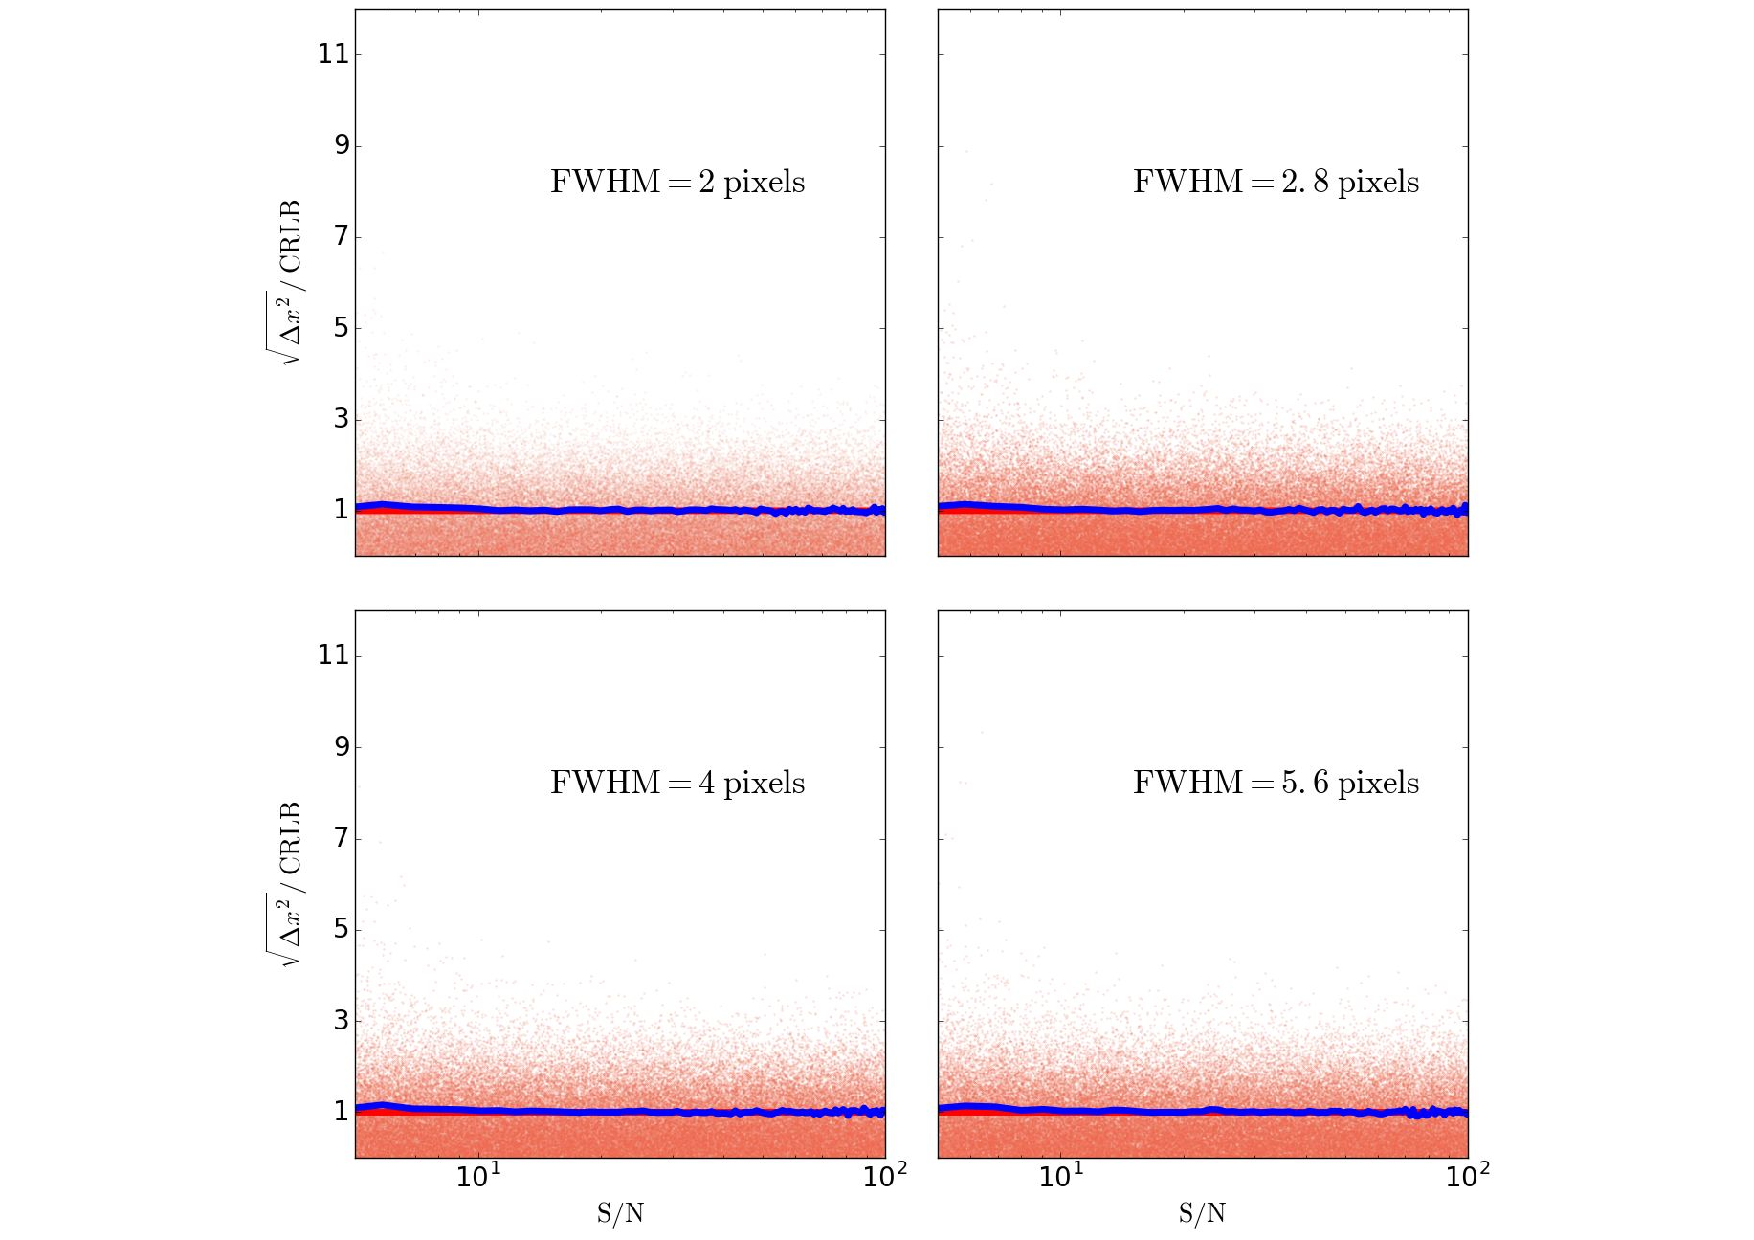
\includegraphics[width=\linewidth]{figures/centroiding/new_psf.pdf}
%\endminipage
\caption{Scatter plots showing the relation between the ratio of error (in x-axis of the centroid poistions) to the CRLB and the signal-to-noise ratio of stars. 
Errors are found from fitting the exact PSF model to the stars,
with FWHM of : 2 (upper left), 2.8 (upper right), 4 (lower left), and 5.6 (lower right)
pixels. In each scatter plot, the blue solid line represents the ratio of the root-mean-squared-error to the CRLB, and the red line represents the ratio achievable by an optimal estimator.}\label{1}
\end{center}
\end{figure*}

\begin{figure*}[p]~\\
\begin{center}
 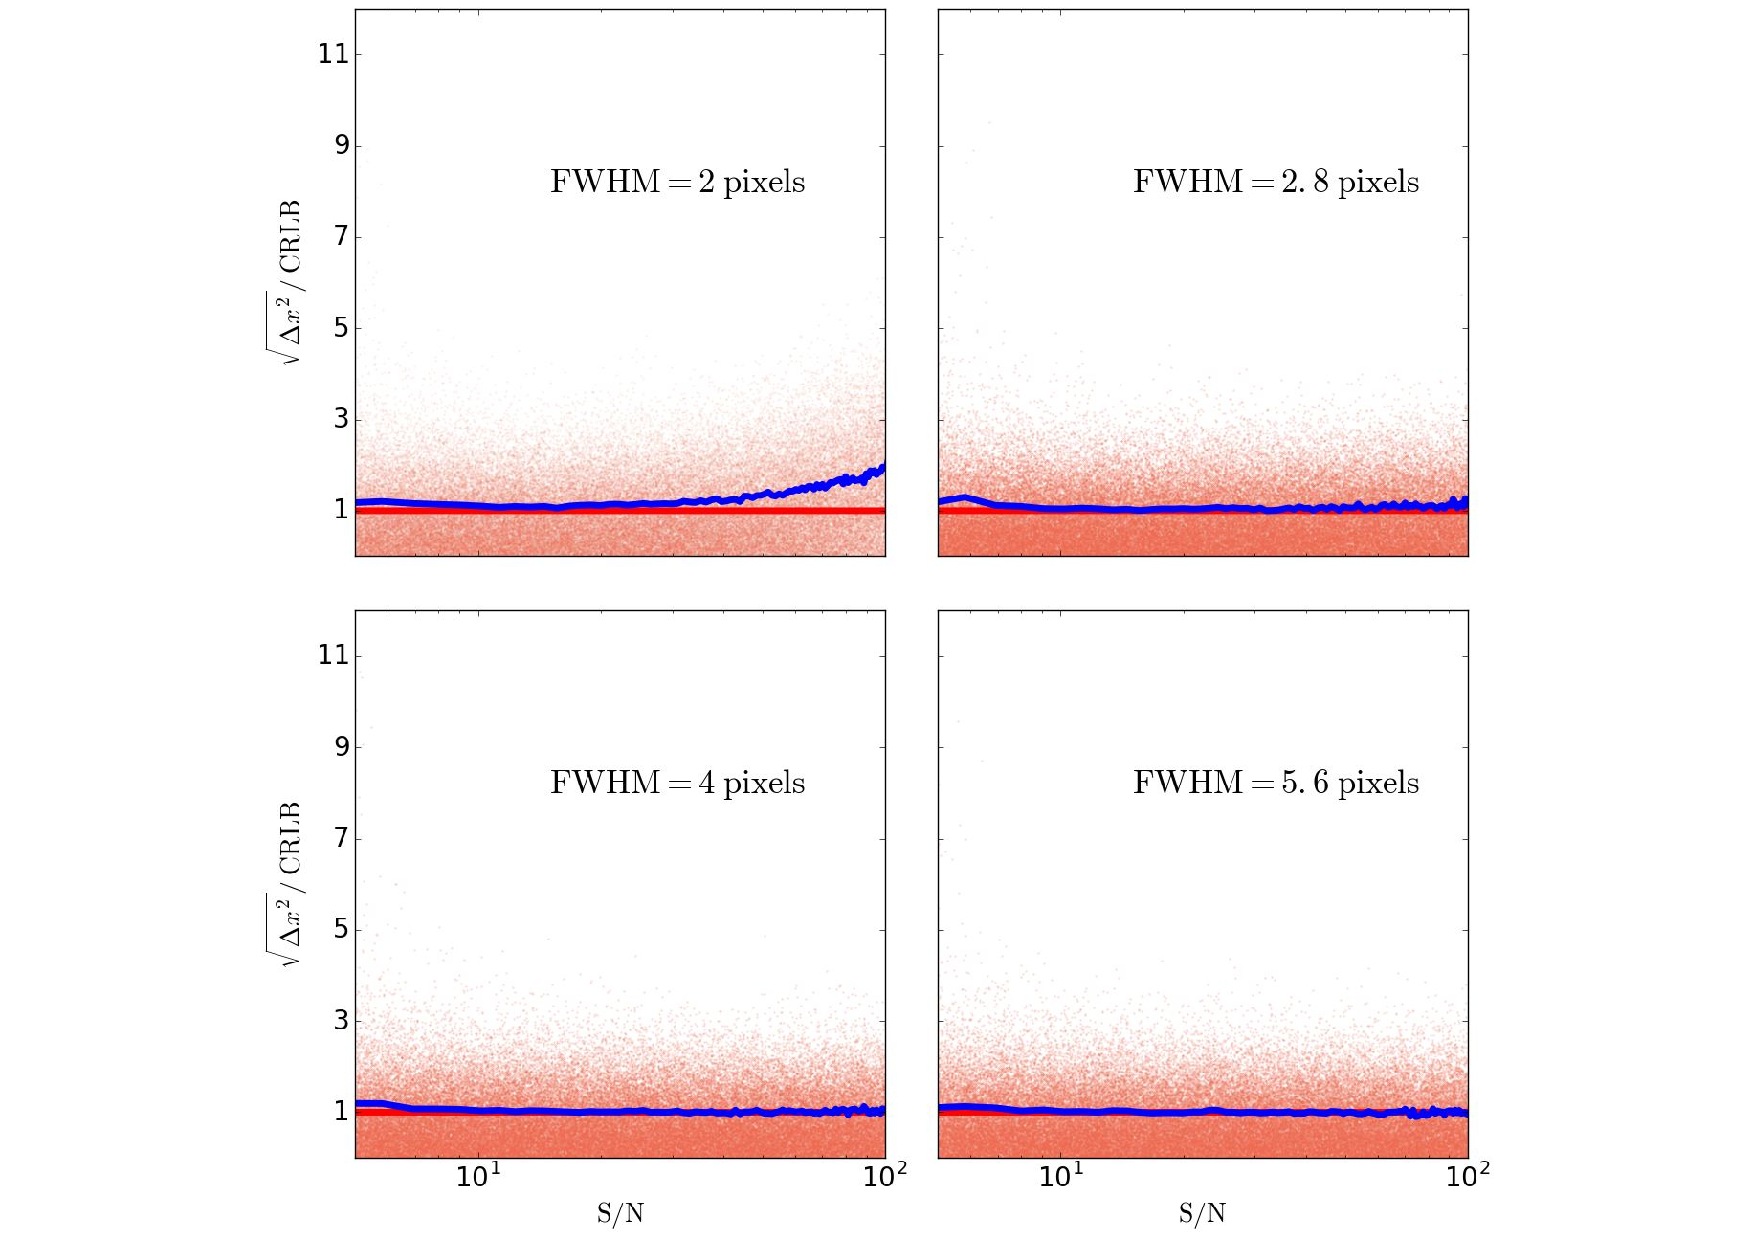
\includegraphics[width=\linewidth]{figures/centroiding/new_matchedfilter.pdf}
%\endminipage
 \caption{
 Scatter plots showing the relation between the ratio of error (in x-axis of the centroid poistions) to the CRLB and the signal-to-noise ratio of stars. 
Errors are found from applying the matched filter polynomial centroiding to the stars,
with FWHM of : 2 (upper left), 2.8 (upper right), 4 (lower left), and 5.6 (lower right) pixels. In each scatter plot, the blue solid line represents the ratio of the root-mean-squared-error to the CRLB, and the red line represents the ratio achievable by an optimal estimator.}\label{2}
\end{center}
\end{figure*}

\begin{figure*}[p]~\\
\begin{center}
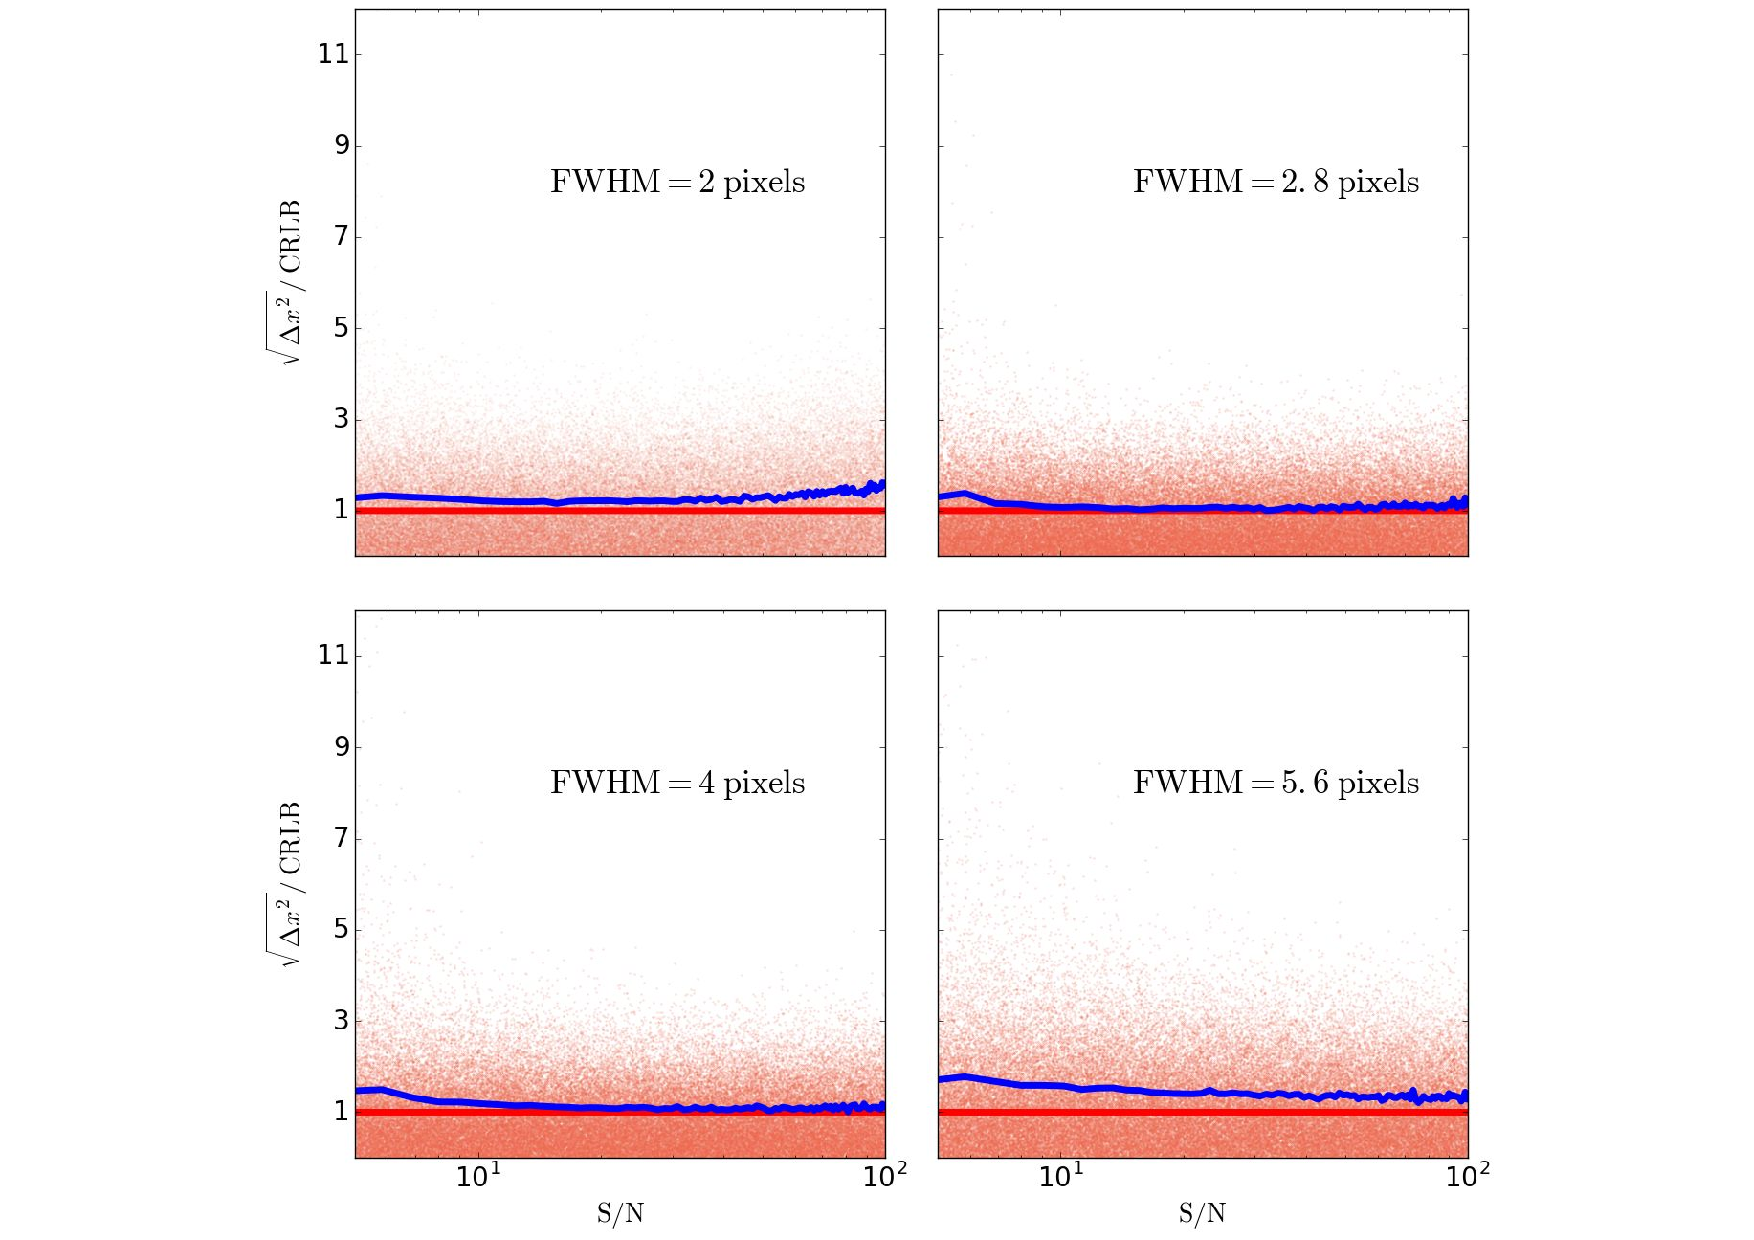
\includegraphics[width=\linewidth]{figures/centroiding/new_polynomial.pdf}
%\endminipage 
\caption{Scatter plots showing the relation between the ratio of error (in x-axis of the centroid poistions) to the CRLB and the signal-to-noise ratio of stars. 
Errors are found from applying the fixed-Gaussian polynomial centroiding to the stars,
with FWHM of : 2 (upper left), 2.8 (upper right), 4 (lower left), and 5.6 (lower right) pixels. In each scatter plot, the blue solid line represents the ratio of the root-mean-squared-error to the CRLB, and the red line represents the ratio achievable by an optimal estimator.}\label{3}
\end{center}
\end{figure*}

\begin{figure*}[p]~\\
\begin{center}
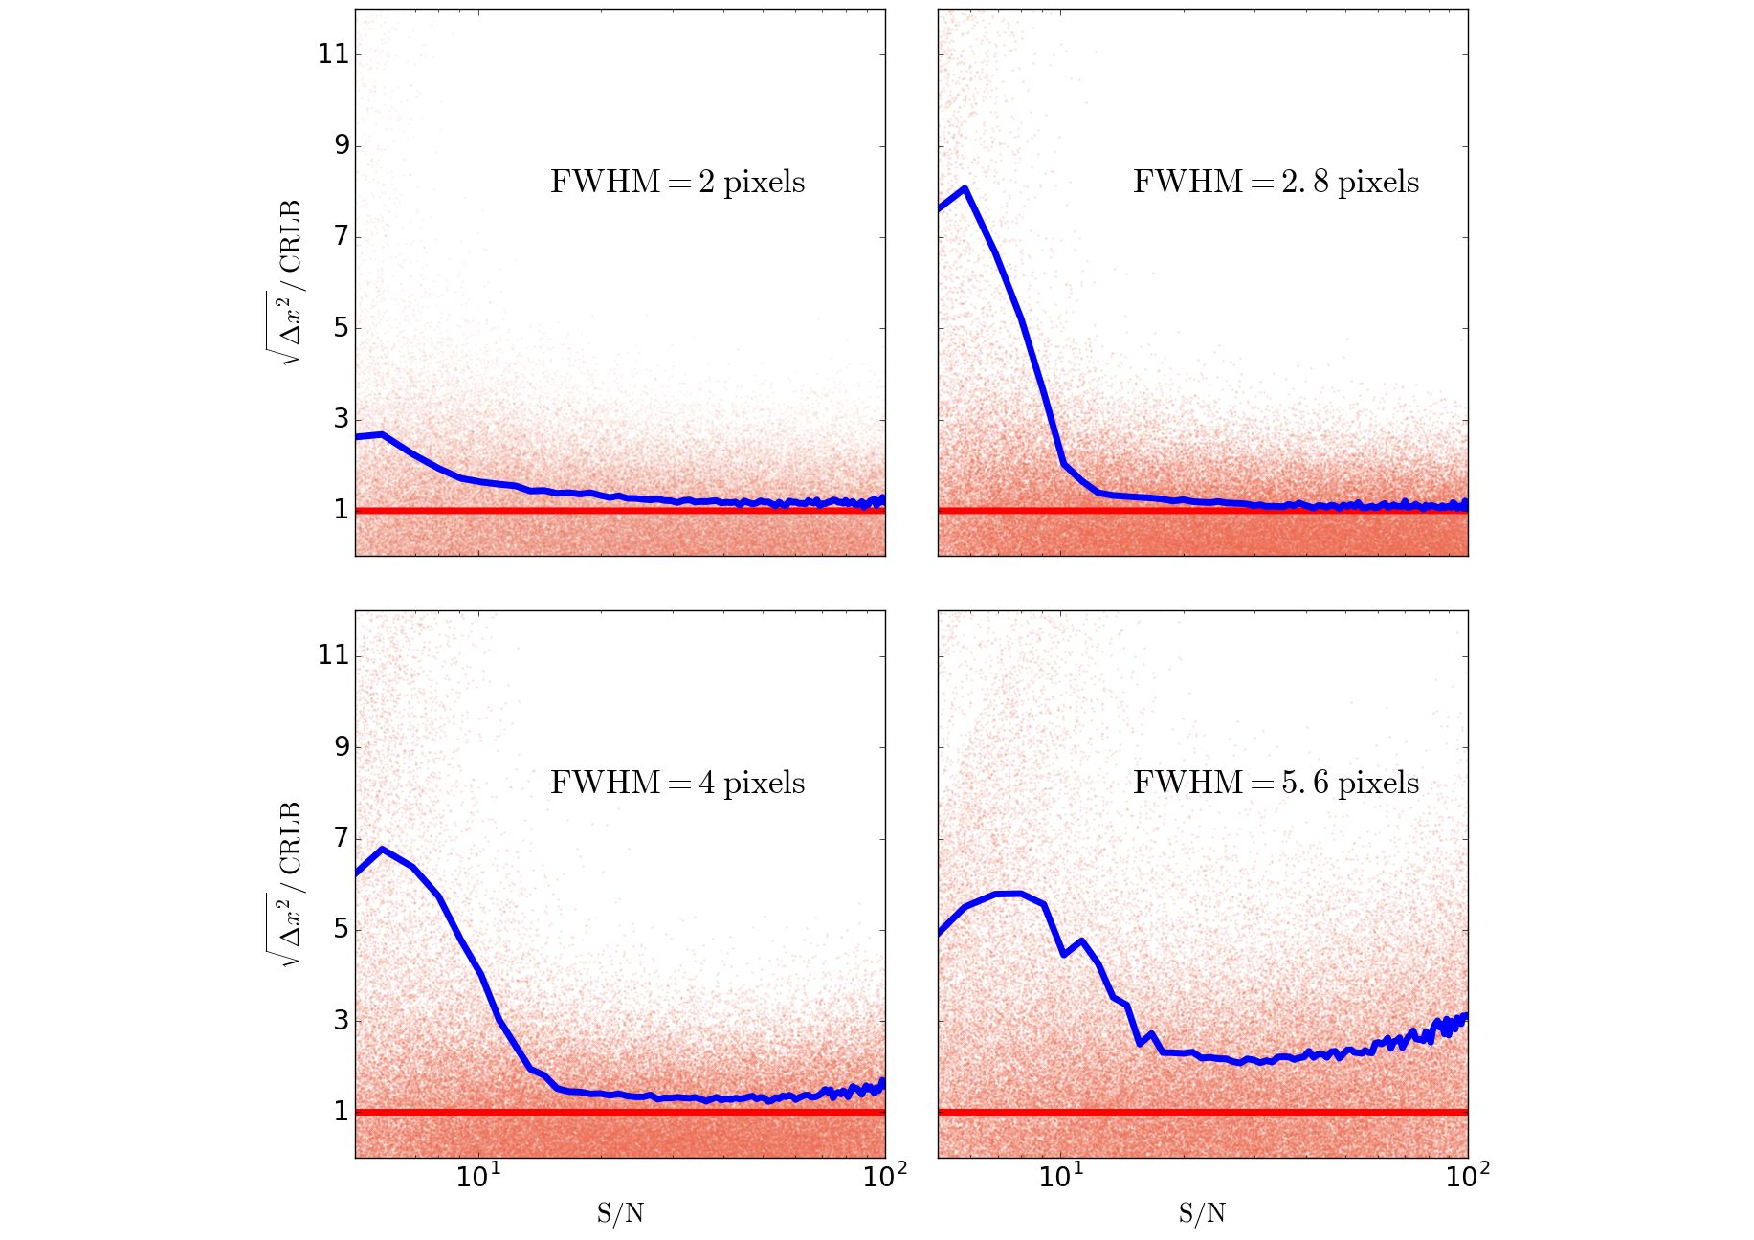
\includegraphics[width=\linewidth]{figures/centroiding/new_moment.pdf}
\caption{Scatter plots showing the relation between the ratio of error (in x-axis of the centroid poistions) to the CRLB and the signal-to-noise ratio of stars. 
Errors are found from applying the 7$\times$7 moment method to the stars,
with FWHM of : 2 (upper left), 2.8 (upper right), 4 (lower left), and 5.6 (lower right) pixels. In each scatter plot, the blue solid line represents the ratio of the root-mean-squared-error to the CRLB, and the red line represents the ratio achievable by an optimal estimator.}\label{4}
\end{center}
\end{figure*}

%%%%%%%%%%%%%%%%%%%%%%%%%%%%%%%%%%%%%%%%%%%%%%%%%%%%%%%%%%%%%%%%%%%%%%%%%%% FWHM PLOTS %%%%%%%%%%%%%%%%%%%%%%%%%%%%%%%%%%%%%%%%%%

\begin{figure*}[p]~\\
\begin{center}
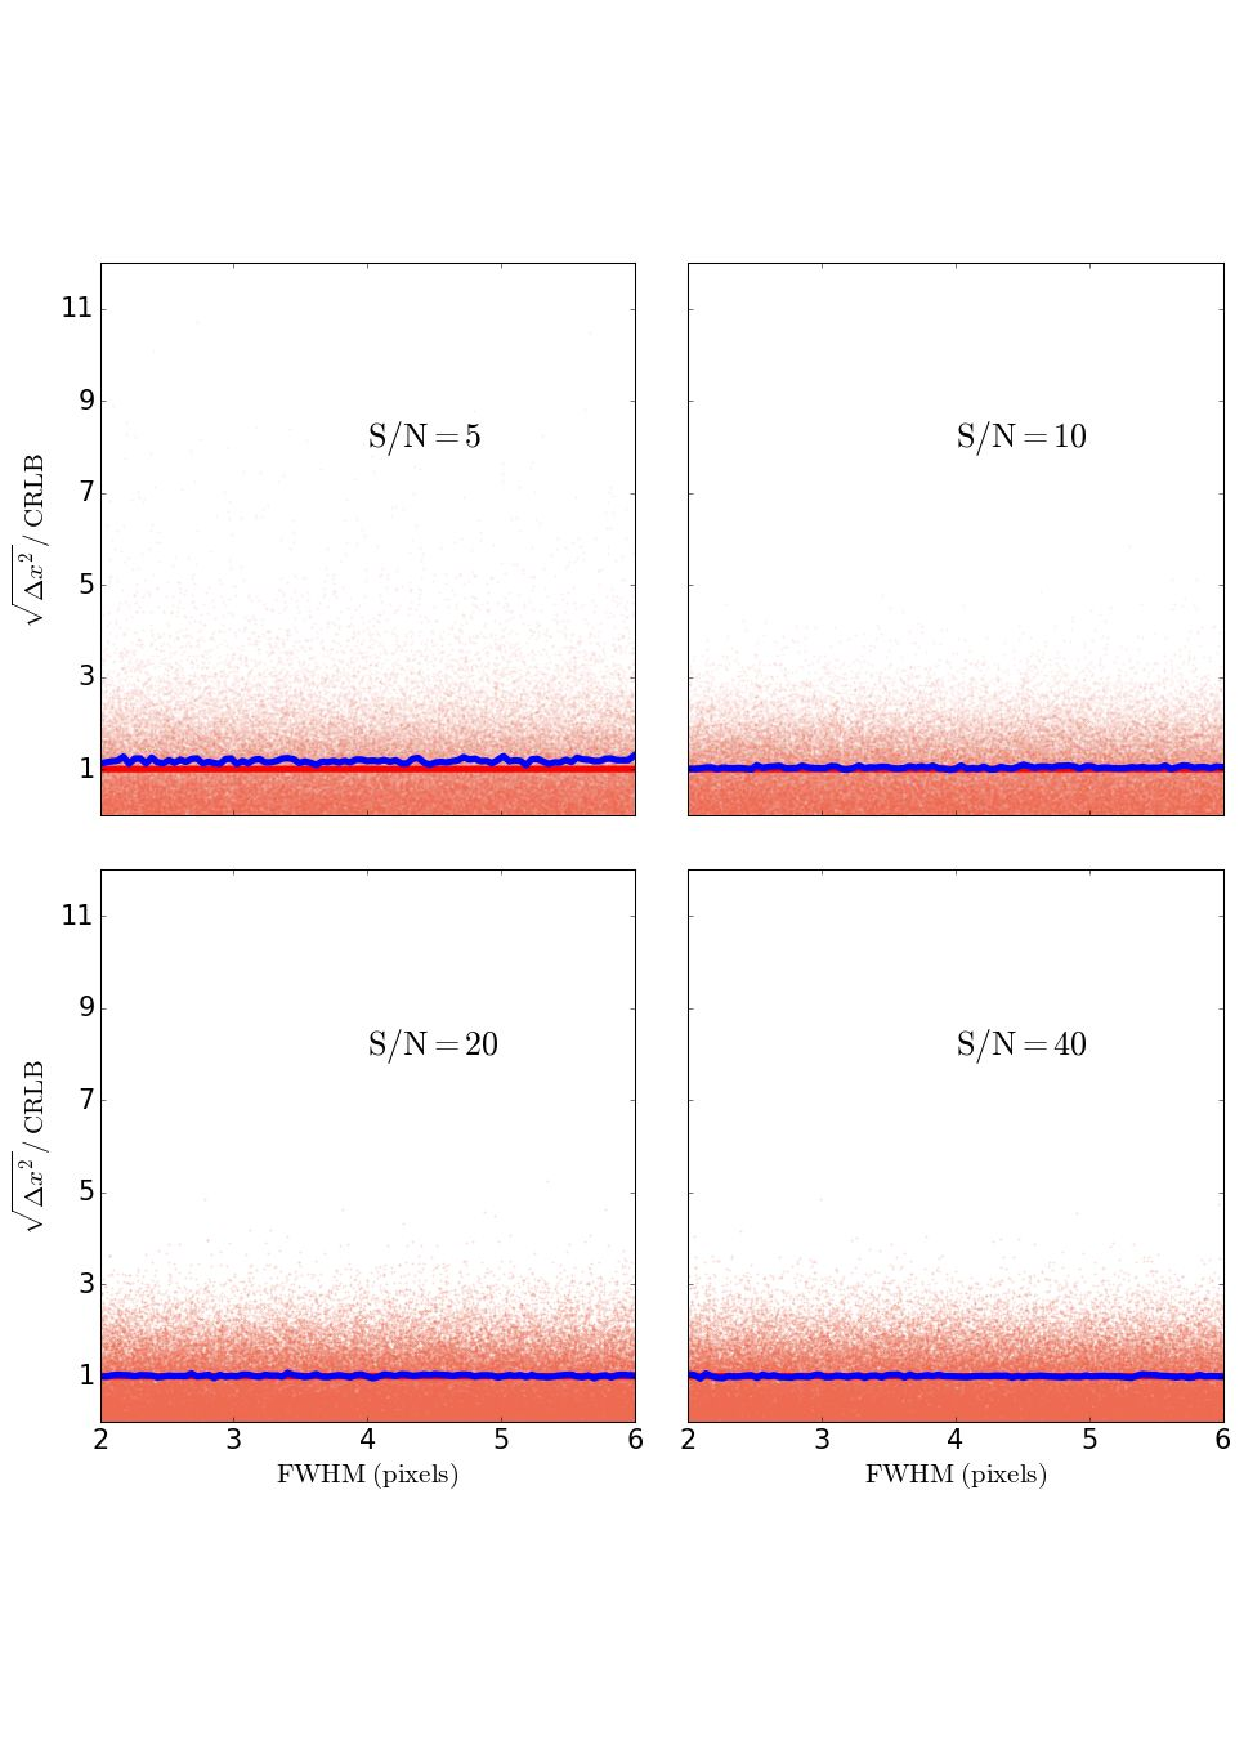
\includegraphics[width=0.65\linewidth]{figures/centroiding/new_fwhm_psf.pdf}
\caption{Scatter plots showing the relation between the ratio of error (in x-axis of the centroid poistions) to the CRLB and the FWHM of stars.
Errors are found from fitting the exact PSF model to the stars, with SNR  of : 5 (upper left), 10 (upper right), 20 (lower left), and 40 (lower right). In each scatter plot, the blue solid line represents the ratio of the root-mean-squared-error to the CRLB, and the red line represents the ratio achievable by an optimal estimator.}\label{5}
\end{center}
\end{figure*}

\begin{figure*}[p]~\\
\begin{center}
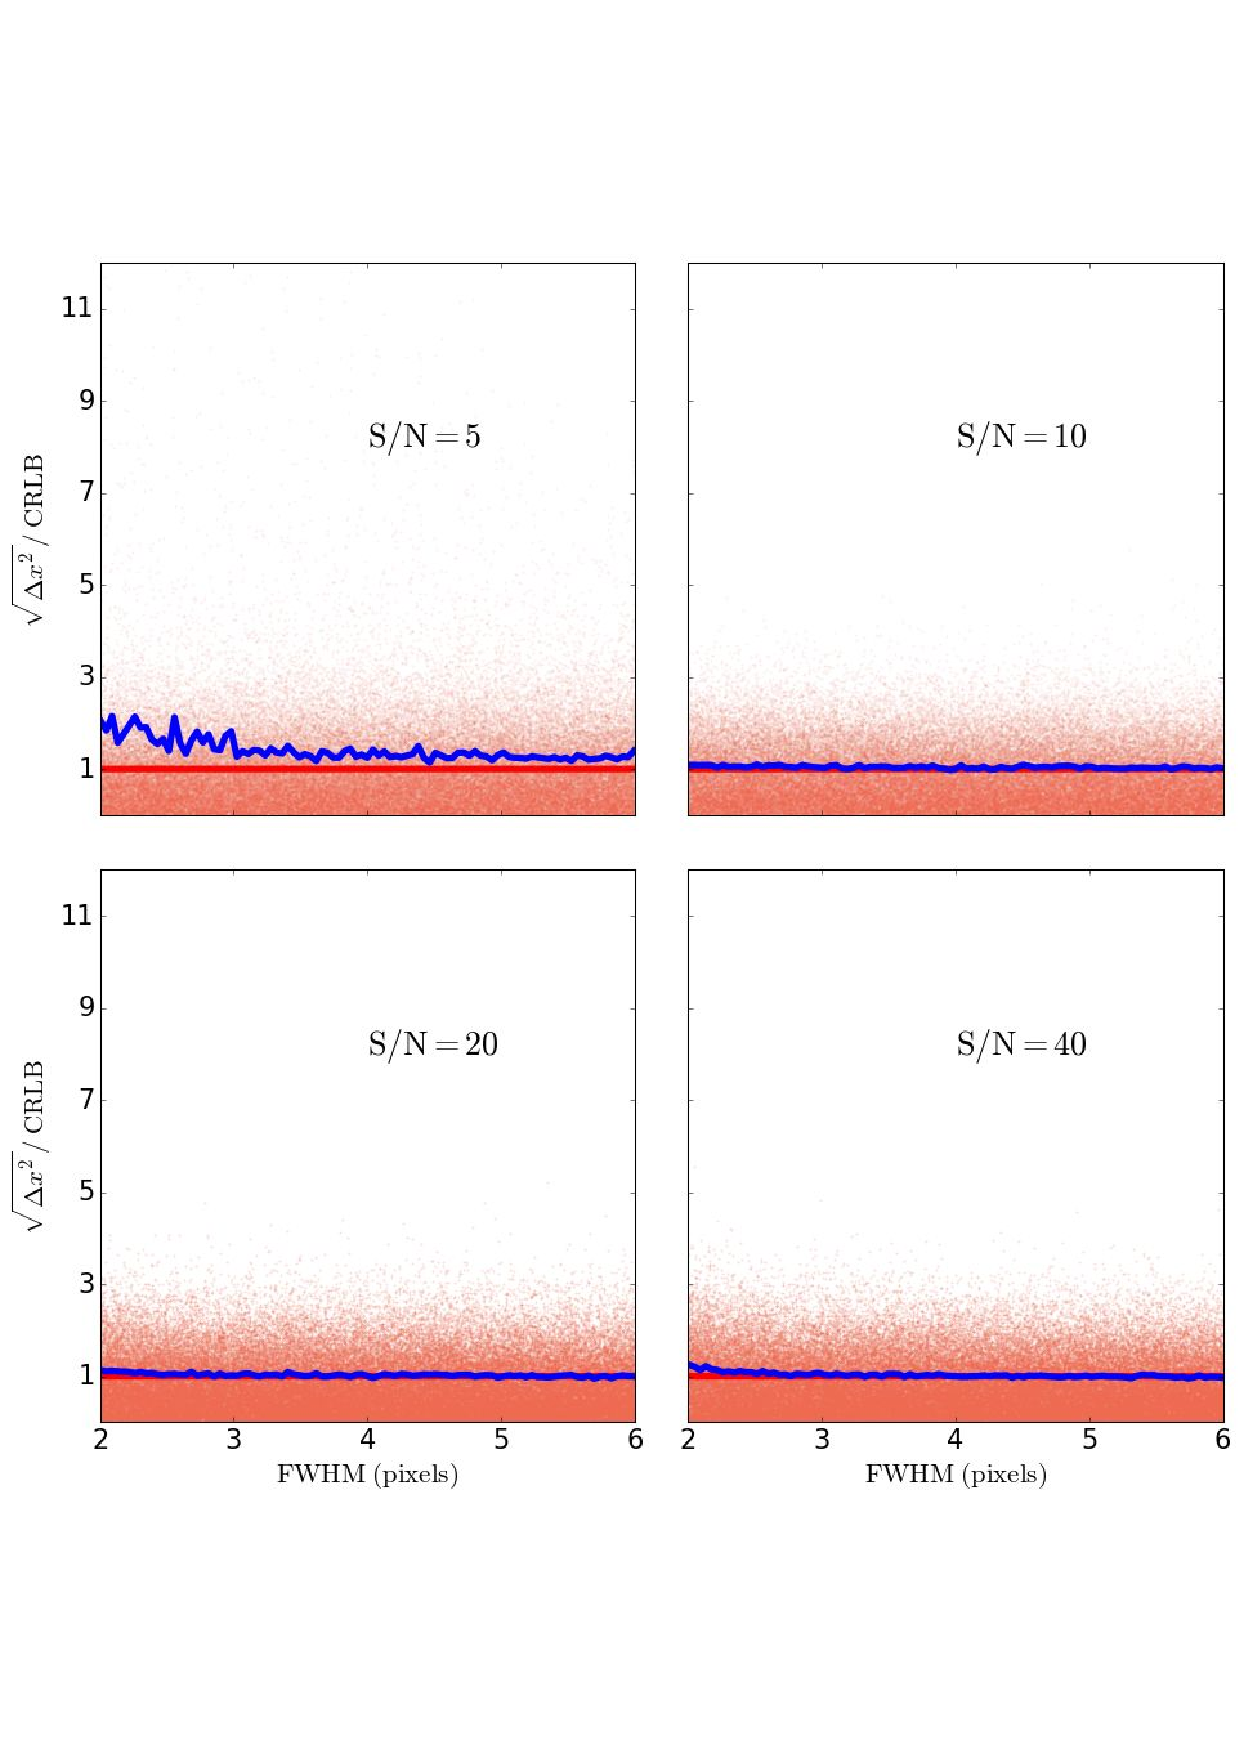
\includegraphics[width=0.65\linewidth]{figures/centroiding/new_fwhm_matchedfilter.pdf}
%\endminipage
\caption{Scatter plots showing the relation between the ratio of error (in x-axis of the centroid poistions) to the CRLB and the FWHM of stars.
Errors are found from applying the matched filter polynomial centroiding to the stars, with SNR  of : 5 (upper left), 10 (upper right), 20 (lower left), and 40 (lower right). In each scatter plot, the blue solid line represents the ratio of the root-mean-squared-error to the CRLB, and the red line represents the ratio achievable by an optimal estimator.}\label{6}
\end{center}
\end{figure*}

\begin{figure*}[p]~\\
\begin{center}
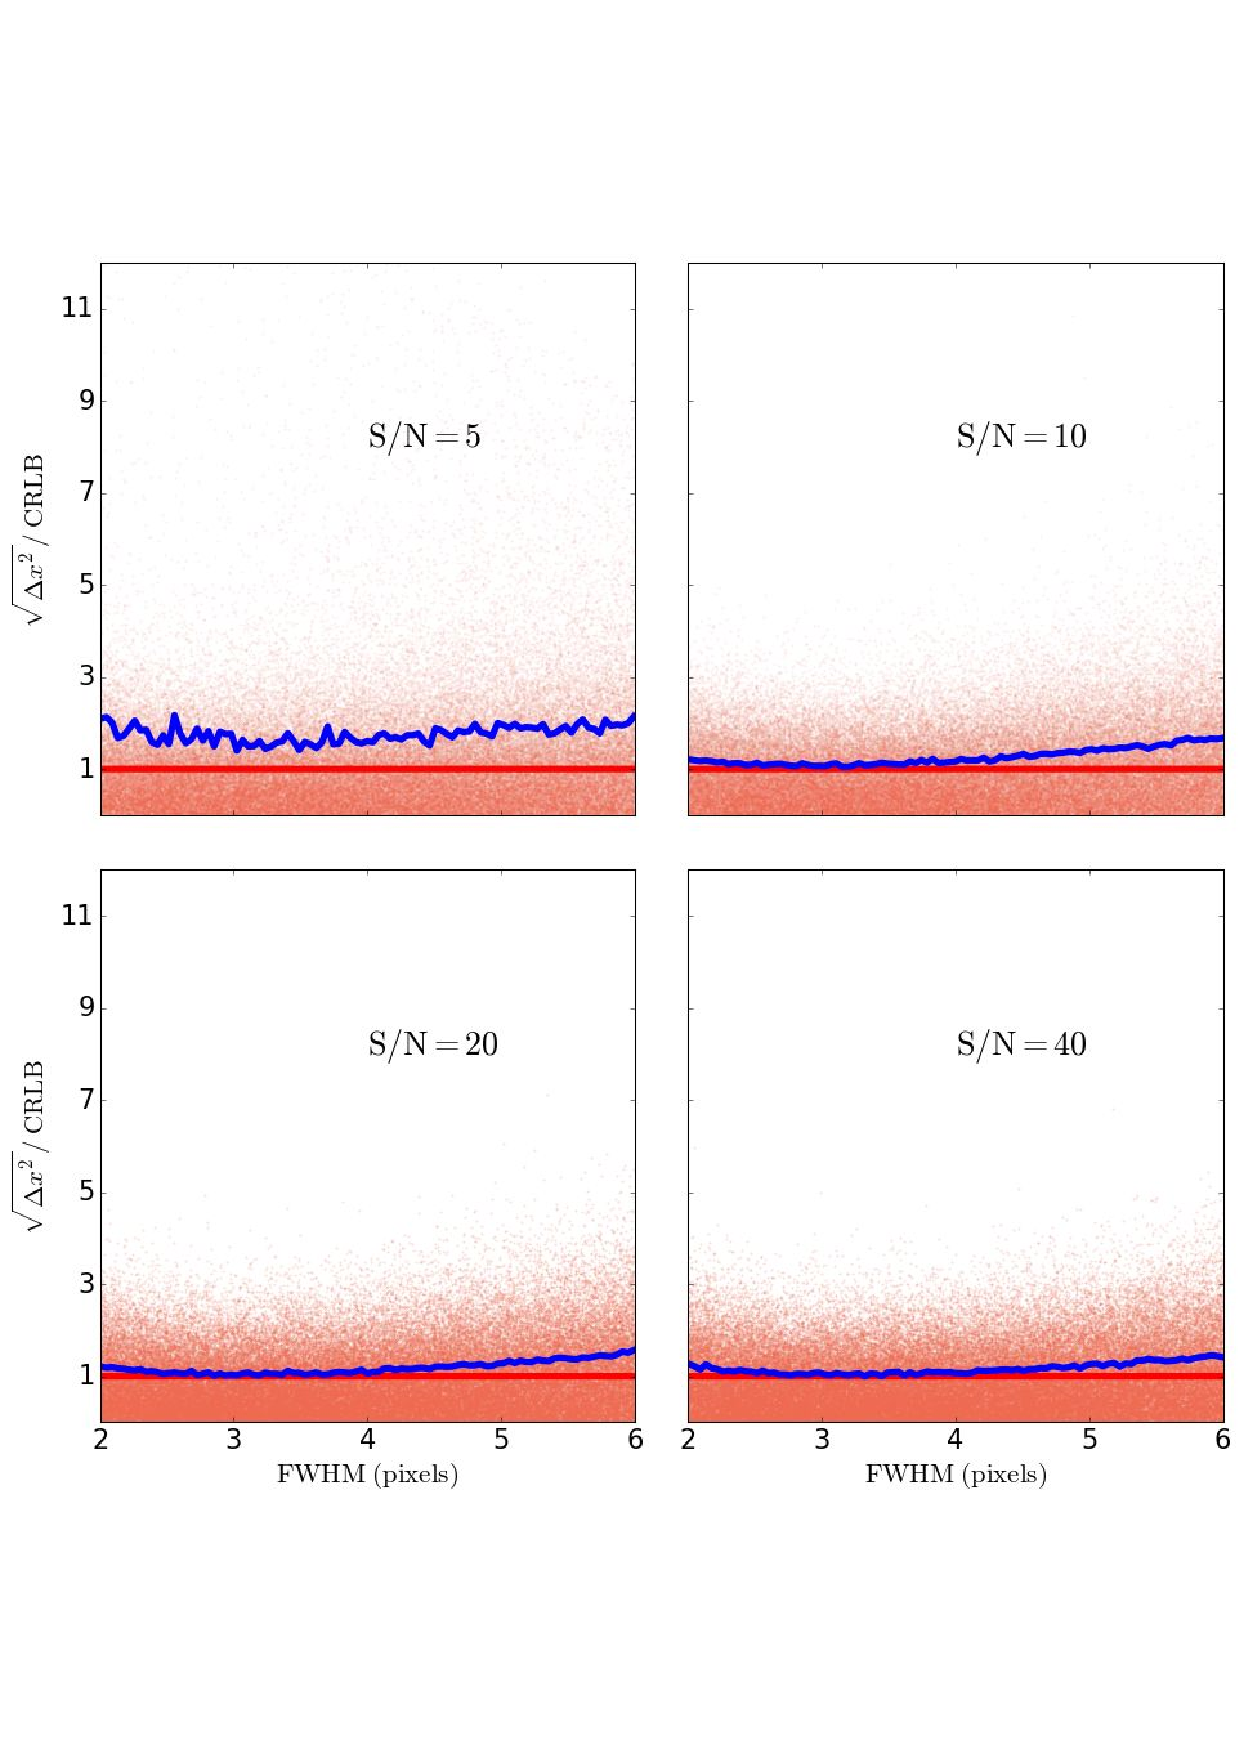
\includegraphics[width=0.65\linewidth]{figures/centroiding/new_fwhm_polynomial.pdf}
%\endminipage
\caption{Scatter plots showing the relation between the ratio of error (in x-axis of the centroid poistions) to the CRLB and the FWHM of stars.
Errors are found from applying the fixed-Gaussian polynomial centroiding to the stars, with SNR  of : 5 (upper left), 10 (upper right), 20 (lower left), and 40 (lower right). In each scatter plot, the blue solid line represents the ratio of the root-mean-squared-error to the CRLB, and the red line represents the ratio achievable by an optimal estimator.}\label{7}
\end{center}
\end{figure*}

\begin{figure*}[p]~\\
\begin{center}
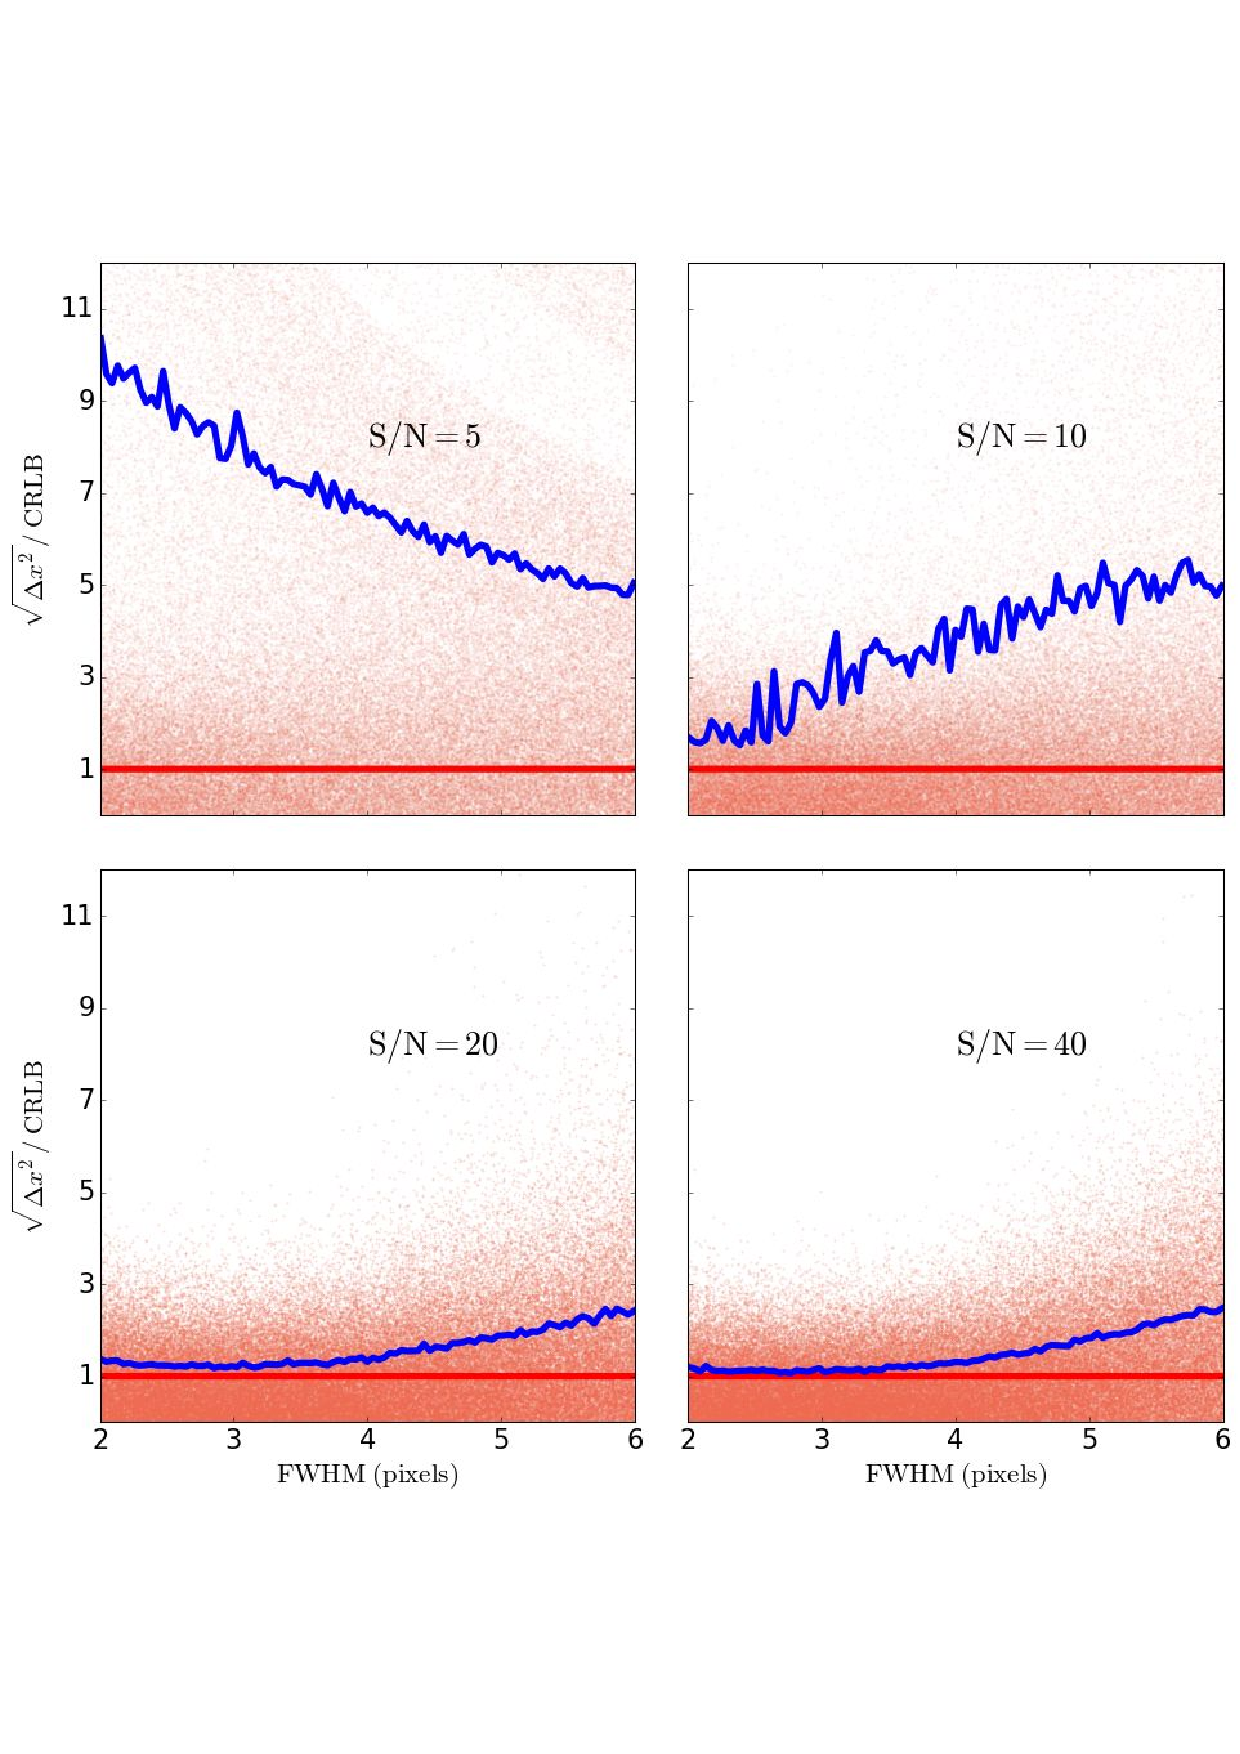
\includegraphics[width=0.65\linewidth]{figures/centroiding/new_fwhm_moment.pdf}
%\endminipage
\caption{Scatter plots showing the relation between the ratio of error (in x-axis of the centroid poistions) to the CRLB and the FWHM of stars.
Errors are found from applying the 7$\times$7 moment method to the stars, with SNR  of : 5 (upper left), 10 (upper right), 20 (lower left), and 40 (lower right). In each scatter plot, the blue solid line represents the ratio of the root-mean-squared-error to the CRLB, and the red line represents the ratio achievable by an optimal estimator.}\label{8}
\end{center}
\end{figure*}

%\bibliographystyle{yahapj}
%\begin{bibliography}
%\bibliography{centroid}
%\end{bibliography}
%\end{document}




\definecolor{dred}{rgb}{0.75,0.,0.}
\definecolor{darkred}{rgb}{0.5,0.,0.}
\definecolor{darkgreen}{rgb}{0.,0.5,0.}

\newcommand{\todo}[1]{{\em \textcolor{red}{ #1}}}
\newcommand{\beq}{\begin{equation}}
\newcommand{\eeq}{\end{equation}}
\newcommand{\lang}{\langle}
\newcommand{\ra}{\rangle}
\newcommand{\vep}{\bm{\epsilon}}
\newcommand{\ep}{\epsilon}
\newcommand{\pars}{\vec{\theta}}
\newcommand{\dev}{\mathrm{d}}
\newcommand{\mstar}{h^{-1}M_\odot}



\chapter{Approximate bayesian computation in large scale structure: constraining the galaxy halo connection \chaplabel{abc}}

This \paper\ is joint work with ChangHoon~Hahn (NYU), Kilian~W.~Walsh (NYU), Andrew~Hearin (Yale), David~W.~Hogg (NYU), and Duncan~Campbell (Yale). 
It is revised in response to the referee report and it is resubmitted to \emph{Monthly Royal Astronomical Society Notice}. 

% Abstract of the paper
\section{Section abstract}

Standard approaches to Bayesian parameter inference in large scale 
structure assume a Gaussian functional form (chi-squared form) 
for the likelihood. This assumption, in detail, cannot %They are also limited to analyzing measurements of the two-point correlation function. 
be correct. Likelihood free inferences such as Approximate Bayesian Computation (ABC) 
relax these restrictions and make inference possible without making any 
assumptions on the likelihood. Instead ABC relies on a forward generative model of the data and a metric 
for measuring the distance between the model and data. In this work, we 
demonstrate that ABC is feasible for LSS parameter inference by using it 
to constrain parameters of the halo occupation distribution (HOD) model 
for populating dark matter halos with galaxies.

Using specific implementation of ABC supplemented with Population Monte Carlo
importance sampling, a generative forward model using HOD, and a distance metric 
based on galaxy number density, two-point correlation function, and galaxy group
multiplicity function, we constrain the HOD parameters of mock observation 
generated from selected ``true'' HOD parameters. The parameter constraints we 
obtain from ABC are consistent with the ``true'' HOD parameters, demonstrating that ABC can be reliably  used for parameter inference in LSS. Furthermore, we compare our ABC constraints to constraints we obtain using a pseudo-likelihood function of Gaussian form with MCMC and find consistent HOD parameter constraints. Ultimately our results suggest that ABC can and should be applied in parameter  inference for LSS analyses. 


%%%%%%%%%%%%%%%%%%%%%%%%%%%%%%%%%%%%%%%%%%%%%%%%%%

%%%%%%%%%%%%%%%%% BODY OF PAPER %%%%%%%%%%%%%%%%%%

\section{Introduction}

Cosmology was revolutionized in the 1990s with the introduction of likelihoods---%
pro\-ba\-bil\-ities for the data given the theoretical model---%
for combining data from different surveys and performing principled inferences of
the cosmological parameters (\citealt{White:1996aa, Riess:1998aa}). 
Nowhere has this been more true than in cosmic microwave background (CMB) studies,
where it is nearly possible to analytically evaluate a likelihood function that
involves no (or minimal) approximations (\citealt{Oh:1999aa}, \citealt{Wandelt:2004aa},  
\citealt{Eriksen:2004aa}, \citealt{planckI, planckII}). 

Fundamentally, the tractability of likelihood functions in cosmology flows from
the fact that the initial conditions are exceedingly close to Gaussian in form,
and that many sources of measurement noise are also Gaussian (\citealt{Knox:1995aa}).
Likelihood functions are easier to write down and evaluate when things are closer 
to Gaussian, so at large scales and in the early universe. Hence likelihood analyses 
are ideally suitable for CMB data. 

In large-scale structure (LSS) with galaxies, quasars, and quasar absorption systems as tracers,
formed through nonlinear gravitational evolution and biasing, the likelihood {\em cannot} be Gaussian. 
Even if the initial conditions are perfectly Gaussian, the growth of structure creates non-linearities 
which are non-Gaussian (see \citealt{Bernardeau:2002aa} for a comprehensive review). 
Galaxies form within the density field in some complex manner that is modeled only effectively
(\citealt{Dressler:1980aa, Kaiser:1984aa, Santiago:1992aa, Steidel:1998aa}; see \citealt{somerville15} for a recent review).  
Even if the galaxies were a Poisson sampling of the density field, which they are not (\citealt{Mo:1996aa, Sommerville:2001aa, Casas-Miranda:2002aa}), it would be tremendously difficult to write down even 
an approximate likelihood function (\citealt{devpois}).

The standard approach makes the strong assumption that the likelihood function 
for the data can be approximated by a pseudo-likelihood function that is a Gaussian
probability density in the space of the two-point correlation function estimate. 
It is also typically limited to (density and) two-point correlation 
function (2PCF) measurements, assuming that these measurements constitute 
sufficient statistics for the cosmological parameters. 
As Hogg (in preparation) demonstrates, the assumption of a Gaussian 
pseudo-likelihood function cannot be correct (in detail) at any scale, 
since a correlation function, being related to the 
variance of a continuous field, must satisfy non-trivial positive-definiteness 
requirements. These requirements truncate function space such that the 
likelihood in that function space could never be Gaussian. The failure of this 
assumption becomes more relevant as the correlation function becomes better measured, 
so it is particularly critical on intermediate scales, where neither shot 
noise nor cosmic variance significantly influence the measurement. 

Fortunately, these assumptions are not required for cosmological inferences, 
because high-precision cosmological simulations can be used to directly calculate 
LSS observables. Therefore, we can simulate not just the one- or two-point statistics of the galaxies, but also any higher order statistics that might provide additional constraining power on a model. In principle, there is therefore no strict need to rely on these common but specious analysis  assumptions as it is possible to calculate a likelihood function directly from simulation outputs.

Of course, any naive approach to sufficiently simulating the data would be ruinously
expensive. Fortunately, there are principled, (relatively) efficient methods for 
minimizing computation and delivering correct posterior inferences, using only a 
data simulator and some choices about statistics. 
In the present work, we use Approximate Bayesian Computation---ABC---which provides a \emph{rejection sampling} 
framework that relaxes the assumptions of the traditional approach. 

ABC approximates the posterior probability distribution function (model given the data)
by drawing proposals from the prior over the model parameters, simulating the data from the 
proposals using a forward generative model, and then rejecting the proposals that are beyond 
a certain threshold ``distance'' from the data, based on summary statistics of the data. 
In practice, ABC is used in conjunction with a more efficient sampling operation like 
Population Monte Carlo (PMC; \citealt{smc}). 
PMC initially rejects the proposals from the prior with a relatively large ``distance'' threshold. 
In subsequent steps, the threshold is updated adaptively, and samples from the proposals that have 
passed the previous iteration are subjected to the new, more stringent, threshold criterion (\citealt{abcpmc}). 
In principle, the distance metric can be any positive definite function that compares 
various summary statistics between the data and the simulation.  

In the context of astronomy, this approach has been used in a wide range of topics including 
image simulation calibration for wide field surveys (\citealt{abccosmology}),
the study of the morphological properties of galaxies at high redshifts (\citealt{abcmorphology}),
stellar initial mass function modeling (Cisewski et al. in preparation),
and cosmological inference with  
with weak-lensing peak counts (\citealt{abcwl,abcwl2}), Type Ia Supernovae (\citealt{abcsn}), 
and galaxy cluster number counts (\citealt{cosmoabc}). 

In order to demonstrate that ABC can be tractably applied to parameter estimation in contemporary 
LSS analyses, we narrow our focus to inferring the parameters of a Halo Occupation Distribution (HOD) 
model. The foundation of HOD predictions is the halo model of LSS, that is, 
collapsed dark matter halos are biased tracers of the underlying cosmic density field 
(\citealt{press74, bond91, cooray_sheth2002}). The HOD specifies how the dark matter 
halos are populated with galaxies by modeling the probability that a given halo hosts 
$N$ galaxies subject to some observational selection criteria 
(\citealt{lemson99, seljak2000,scoccimarro2001,berlind_weinberg2002,zheng2005}).
This statistical prescription for connecting galaxies to halos has been remarkably
successful in reproducing the galaxy clustering, galaxy--galaxy lensing, and other 
observational statistics (\citealt{Rodriguez-Torres:2015aa, miyatake15}), and is a 
useful framework for constraining cosmological parameters (\citealt{vdb03, tinker05, cacciato13, more13}) 
as well as galaxy evolution models (\citealt{conroy09, Tinker:2011aa, leauthaud12, behroozi13, Tinker:2013aa}, 
Walsh et al. in preparation). 

More specifically, we limit our scope to a likelihood analysis of HOD model parameter space, 
keeping cosmology fixed. We forward model galaxy survey data by populating pre-built dark 
matter halo catalogs obtained from high resolution N-body simulations (\citealt{bolshoi,multidark}) using 
$\mathtt{Halotools}$\footnote{http://halotools.readthedocs.org} 
(\citealt{Hearin:2016aa}), 
an open-source package for modeling the galaxy-halo connection. 
Equipped with the forward model, we use summary statistics such as 
number density, two-point correlation function, galaxy group multiplicity function (GMF)
to infer HOD parameters using ABC.  

In Section \ref{sec:method} we discuss the algorithm of the ABC-PMC prescription we use in our analyses. 
This includes the sampling method itself, the HOD forward model, and the computation of summary statistics. 
Then in Section \ref{sec:mock_obv}, we discuss the mock galaxy catalog, which we treat as observation. 
With the specific choices of ABC-PMC ingredients, which we describe in Section \ref{sec:abcpmc_spec}, 
in Section \ref{sec:abc_results} we present the results of our parameter inference using 
two sets of summary statistics, number density and 2PCF and number density and GMF. 
We also include in our results, analogous parameter constraints from the standard MCMC approach, 
which we compare to ABC results in detail, Section \ref{sec:abcvsmcmc}. Finally, we discuss and 
conclude in Section \ref{sec:discussion}.


\section{Methods}\label{sec:method}
%%%%%%%%%%%%%%%%%%%%% SECTION %%%%%%%%%%%%%%%%%%%%%%%%%%
% Approximate Bayesian Computation  
%%%%%%%%%%%%%%%%%%%%%%%%%%%%%%%%%%%%%%%%%%%%%%%%%%%%%%%%
\subsection{Approximate Bayesian Computation} \label{sec:abc}
ABC is based on rejection sampling, so we begin this section with a brief overview of 
rejection sampling. Broadly speaking, rejection sampling is a Monte Carlo method 
used to draw samples from a probability distribution, $f(\alpha)$, which is difficult to directly sample. The strategy is to draw samples from an instrumental distribution $g(\alpha)$ that satisfies the condition $f(\alpha) < M g(\alpha)$ for all $\alpha,$ where $M > 1$ is some scalar multiplier. The purpose of the instrumental distribution $g(\alpha)$ is that it is easier to sample than $f(\alpha)$ (see \citealt{bishop} and refernces therein). 

In the context of simulation-based inference, 
the ultimate goal is to sample from the joint probability of a
simulation $X$ and parameters $\pars$ given observed data $D$, the
posterior probability distribution. From Bayes rule this posterior 
distribution can be written as 
\beq
p(\pars, X | D) = \frac{p(D|X)p(X|\pars)\pi(\pars)}{\mathcal{Z}}
\eeq
where $\pi(\pars)$ is the prior distribution over the parameters of 
interest and $\mathcal{Z}$ is the evidence, 
\beq
\mathcal{Z} = \int d\pars \; dX\; p(D|X) p(X|\pars) \pi(\pars), 
\eeq
where the domain of the integral is all possible values of $X$ and $\pars$. 
Since $p(\pars, X | D)$ cannot be directly sampled, we use rejection 
sampling with instrumental distribution 
\beq
q(\pars, X) = p(X|\pars) \pi(\pars)
\eeq
and the choice of 
\beq
M = \frac{\mathrm{max}\; p(D|X)}{\mathcal{Z}} > 1.
\eeq
Note that we do not ever need to know $\mathcal{Z}$. 
The choices of $q(\pars, X)$ and $M$ satisfy the condition 
\beq
p(\pars, X | D) < M q(\pars, X)
\eeq
so we can sample $p(\pars, X | D)$ by drawing ${\pars, X}$ from $q(\pars, X)$.
In practice, this is done 
by first drawing $\pars$ from the prior $\pi(\pars)$ and then generating a 
simulation $X = f(\pars)$ via the forward model. Then ${\pars, X}$ 
is accepted if
\beq \label{eq:reject_samp}
\frac{p(\pars, X | D)}{M q(\pars, X)} = \frac{p(D|X)}{\mathrm{max}\;p(D|X)} > u 
\eeq
where $u$ is drawn from $\mathtt{Uniform}[0,1]$. By repeating this rejection sampling process, 
we sample the distribution $p(\pars, X |D)$ with the set of $\pars$ and $X$ that are accepted. 

At this stage, ABC distinguishes itself by postulating that $p(D|X)$, 
the probability of observing data $D$ given simulation $X$ 
({\em not} the likelihood), is proportional to the 
probability of the distance between the data and the simulation X being less than 
an arbitrarily small threshold $\epsilon$ 
\beq
p(D|X) \propto p(\rho(D,X)<\epsilon)
\label{eq:abc_condition}
\eeq
where $\rho(D, X)$ is the distance between the data $D$ and simulation $X$. 
Eq. \ref{eq:abc_condition} along with the rejection sampling acceptance criteria 
(Eq. \ref{eq:reject_samp}), leads to the acceptance criteria for ABC: $\pars$ is accepted if $\rho(D, X) < \epsilon$. 

The distance function is a positive definite function that measures the closeness 
of the data and the simulation. The distance can be a vector with multiple components 
where each component is a distance between a single summary statistic of the data 
and that of the simulation. In that case, the threshold $\epsilon$ in 
Eq. \ref{eq:abc_condition} will also be a vector with the same dimensions.  
$\pars$ is accepted if the distance vector is less than the threshold vector for 
every component.

The ABC procedure begins, in the same fashion as rejection sampling, by drawing 
$\pars$ from the prior distribution $\pi(\pars)$. The simulation is generated from 
$\pars$ using the forward model, $X = f(\pars)$. Then the distance between 
the data and simulation, $\vec\rho(D, X)$, is calculated and compared to 
$\vec\epsilon$. If $\vec\rho(D, X) < \vec\epsilon$, $\pars$ is accepted. 
This process is repeated until we are left with a sample of $\pars$ that all 
satisfy the distance criteria. This final ensemble approximates the posterior 
probability distribution $p(\pars, X|D)$. 

As it is stated, the ABC method poses some practical challenges. If the 
threshold $\epsilon$ is arbitrarily large, the algorithm essentially 
samples from the prior $\pi(\pars)$. Therefore a sufficiently small threshold
is necessary to sample from the posterior probability distribution. However,
an appropriate value for the threshold is not known \emph{a priori}. Yet, 
even if an appropriate threshold is selected, a small threshold requires 
the entire process to be repeated for many draws of $\pars$ from $\pi(\pars)$ 
until a sufficient sample is acquired. This often presents computation challenges. 

We overcome some of the challenges posed by the above ABC method
by using a Population Monte Carlo (PMC) algorithm as our sampling technique. 
PMC is an iterative method that performs rejection sampling over a 
sequence of $\pars$ distributions ($\{p_1(\pars), ..., p_T(\pars)\}$ for 
$T$ iterations), with a distance threshold that decreases at each iteration of 
the sequence. 

\begin{algorithm} 
\caption{The procedure for ABC-PMC}
\begin{algorithmic}[1] \label{alg:abcpmc}
%\STATE \DATA: D
%\STATE \RESULT: ABC posterior sample of $\pars$
\IF{$t=1:$}
%\STATE $\epsilon_t \gets \infty$
\FOR{$i=1,...,N$}
   \STATE // \emph{This loop can now be done in parallel for all i}
   \WHILE{$\rho(X,D)>\epsilon_t$}
   \STATE $\pars^{*}_{t} \gets \pi(\pars)$
   \STATE $X = f(\pars^{*}_{t})$
   \ENDWHILE
   \STATE $\pars^{(i)}_{t} \gets \pars^{*}_{t}$
   \STATE $w^{(i)}_{t} \gets 1/N$
\ENDFOR
\ENDIF
\IF{$t=2,...,T:$}
\FOR{$i=1,...,N$}
   \STATE // \emph{This loop can now be done in parallel for all i}
   \WHILE{$\rho(X,D)>\epsilon_t$}
   \STATE Draw $\pars^{*}_{t}$ from $\{\pars_{t-1}\}$ with probabilities $\{w_{t-1}\}$
   \STATE $\pars^{*}_{t} \gets K(\pars^{*}_{t},.)$
   \STATE $X = f(\pars^{*}_{t})$
   \ENDWHILE
   \STATE $\pars^{(i)}_{t} \gets \pars^{*}_{t}$
   \STATE $w^{(i)}_{t} \gets \pi(\pars^{(i)}_{t}) / \big(\sum\limits_{j=1}^{N}w_{t-1}^{(i)}K(\pars^{(j)}_{t-1},\pars^{(i)}_{t}) \big)$
\ENDFOR
\ENDIF
\end{algorithmic}
\end{algorithm}

As illustrated in Algorithm \ref{alg:abcpmc}, for the first iteration $t = 1$, 
we begin with an arbitrarily large distance threshold $\epsilon_1$. We 
draw $\pars$ (hereafter referred to as particles) from the prior distribution 
$\pi(\pars)$. We forward model the simulation $X = f(\pars)$, calculate the 
distance $\rho(D, X)$, compare this distance to $\epsilon_1$, and then 
accept or reject the $\pars$ draw. Because we set $\epsilon_1$ arbitrarily large, 
the particles essentially sample the prior distribution. This process 
is repeated until we accept $N$ particles. We then assign equal weights to 
the $N$ particles: $w_1^i = 1/N$.

For subsequent iterations ($t > 1$) the distance threshold is set such that
$\epsilon_{i,t} < \epsilon_{i,t-1}$ for all components $i$. Although there is 
no general prescription, the distance threshold $\epsilon_{i,t}$ can be 
assigned based on the empirical distribution of the accepted distances of the 
previous iteration, $t-1$. In \citealt{abcsn}, for instance, the threshold of 
the second iteration is set to the $25^\mathrm{th}$ percentile of the distances 
in the first iterations; afterwards in the subsequent iterations, $t$, $\epsilon_{t}$ 
is set to the $50^\mathrm{th}$ percentile of the distances in the previous $t-1$ iteration. 
Alternatively, \citealt{abcwl} set $\epsilon_{t}$ to the median of the distances from 
the previous iteration. In Section \ref{sec:abcatwork}, we describe our prescription 
for the distance threshold, which follows \citealt{abcwl}. 

Once $\epsilon_t$ is set, we draw a particle from the previous 
weighted set of particles ${\pars}_{t-1}$. 
This particle is perturbed by a kernel, set to the covariance of ${\pars}_{t-1}$.
Then once again, we generate a simulation by forward modeling $X = f(\pars^i)$, 
calculate the distance $\rho(X, D)$, and compare the distance to the new distance 
threshold ($\epsilon_t$) in order to accept or reject the particle. This process is 
repeated until we assemble a new set of $N$ particles ${\pars}_t$. We then update the 
particle weights according to the kernel, the prior distribution, and the 
previous set of weights, as described in Algorithm \ref{alg:abcpmc}. The 
entire procedure is then repeated for the next iteration, $t+1$.

There are a number of ways to specify the perturbation kernel in the ABC-PMC algorithm. 
A widely used technique is to define the perturbation kernel as a multivariate Gaussian 
centered on the weighted mean of the particle population with a covariance matrix set to 
the covariance of the particle population. This perturbation kernel is often called the 
global multivariate Gaussian kernel. For a thorough discussion of various schemes for 
specifying the perturbation kernel, we refer the reader to \citealt{optimalkernel}. 

The iterations continue in the ABC-PMC algorithm until convergence is confirmed. 
One way to ensure convergence is to impose a threshold for the acceptance ratio, 
which is measured in each iteration. The acceptance ratio is the ratio of the number 
of proposals accepted by the distance threshold, to the full number 
of proposed particles at every step. Once the acceptance ratio for 
an iteration falls below the imposed threshold, the algorithm has converged and is
suspended. Another way to ensure convergence is by monitoring the fractional change in 
the distance threshold ($\epsilon_t/\epsilon_{t-1} - 1$)
after each iteration. When the fractional change becomes smaller than some 
specified tolerance level, the algorithm has reached convergence. Another 
convergence criteria, is through the derived uncertainties of the inferred
parameters measured after each iteration. When the uncertainties stabilize 
and show negligible variations, convergence is ensured. In Section \ref{sec:abcpmc_spec} 
we detail the specific convergence criteria used in our analysis. 

\subsection{Forward model}\label{sec:forwardmodel}
\subsubsection{Halo Occupation Modeling}

\newcommand{\lcdm}{\Lambda {\rm CDM}}
\newcommand{\dd}{\mathrm{d}}
\newcommand{\mean}[2]{\left\langle#1 \vert {#2}\right\rangle}

%%% HALO OCCUPATION DISTRIBUTION %%%
\newcommand{\ngal}{N_{\mathrm{g}}}
\newcommand{\nsat}{N_\mathrm{s}}
\newcommand{\ncen}{N_\mathrm{c}}
\newcommand{\pnm}[2]{p(#1|#2)}

\newcommand{\mhalo}{M_{\rm h}}
\newcommand{\mvir}{M_\mathrm{vir}} 

\newcommand{\dndmvir}{\frac{\dd n}{\dd\mvir}}
\newcommand{\dndmhalo}{\frac{\dd n}{\dd\mhalo}}
\newcommand{\dndmvirprime}{\frac{\dd n}{\dd\mvir'}}

%%% CLUSTERING STATISTICS %%%
\newcommand{\xigg}{\xi_{\mathrm{gg}}}
\newcommand{\xihh}{\xi_{\mathrm{hh}}}
\newcommand{\xiggr}{\xi_{\mathrm{gg}}(r)}
\newcommand{\xiggroneh}{\xi^{1h}_{\mathrm{gg}}(r)}
\newcommand{\xiggrtwoh}{\xi^{2h}_{\mathrm{gg}}(r)}
\newcommand{\ngalaxy}{\bar{n}_{\mathrm{g}}}
\newcommand{\gmf}{\mathcal{\zeta}_{\rm g}}

ABC requires a forward generative model. In large scale structure studies, this implies a model
that is able to generate a galaxy catalog. We then calculate and compare summary statistics of the data and model catalog in an identical fashion
In this section, we describe the forward generative model we use within the framework of the 
halo occupation distribution.

The assumption that galaxies reside in dark matter halos is the bedrock underlying 
all contemporary theoretical predictions for galaxy clustering. The Halo Occupation Distribution 
(HOD) is one of the most widely used approaches to characterizing this galaxy-halo connection. 
The central quantity in the HOD is $\pnm{\ngal}{\mhalo}$, the probability that a halo of mass 
$\mhalo$ hosts $\ngal$ galaxies. 

The most common technical methods for estimating the theoretical galaxy 2PCF utilize the 
first two moments of $P$, which contain the necessary information to calculate the one- 
and two-halo terms of the galaxy correlation function:
\begin{eqnarray}
\label{eq:onehaloterm}
1+\xiggroneh \simeq \frac{1}{4\pi{}r^{2}\ngalaxy^{2}}\int\dd\mhalo\dndmhalo\Xi_{\rm gg}(r|\mhalo) \times \mean{\ngal(\ngal-1)}{\mhalo},
\end{eqnarray} and

\begin{eqnarray}
\label{eq:twohaloterm}
\xiggrtwoh \simeq \xi_{\mathrm{mm}}(r)\left[\frac{1}{\ngalaxy}\int\dd\mhalo\dndmhalo \mean{\ngal}{\mhalo}b_{\mathrm{h}}(\mhalo)\right]^{2}
\end{eqnarray}
In Eqs.~(\ref{eq:onehaloterm}) and (\ref{eq:twohaloterm}), $\ngalaxy$ is the galaxy number density,
$\dd\mathrm{n}/\dd\mhalo$ is the halo mass function, the spatial bias of dark matter halos is 
$b_{\mathrm{h}}(\mhalo),$ and $\xi_{\rm mm}$ is the correlation function of dark matter.  
If we represent the spherically symmetric intra-halo distribution of galaxies by a unit-normalized 
$n_{\rm g}(r),$ then the quantity $\Xi_{\rm gg}(r)$ appearing in the above two equations 
is the convolution of $n_{\rm g}(r)$ with itself. These fitting functions are calibrated using $N$-body 
simulations. 

Fitting function techniques, however, require many simplifying assumptions. For example, 
Eqs.~(\ref{eq:onehaloterm}) and (\ref{eq:twohaloterm}) assume that the galaxy 
distribution within a halo is spherically symmetric. These equations 
also face well-known difficulties of properly treating halo exclusion and scale-dependent bias, 
which results in additional inaccuracies commonly exceeding the $10\%$ level (\citealt{vdBosch13}). 
Direct emulation methods have made significant improvements in precision and accuracy in recent 
years (\citealt{coyote2,coyote1}); however, a labor- and computation-intensive interpolation 
exercise must be carried out each time any alternative statistic is explored, which is one of the goals of the present work.

To address these problems, throughout this paper we make no appeal to fitting functions or emulators. 
Instead, we use the $\mathtt{Halotools}$ package to populate dark matter halos with mock galaxies and 
then calculate our summary statistics directly on the resulting galaxy catalog with the same estimators 
that are used on observational data (\citealt{Hearin:2016aa}). Additionally, through our forward modeling approaching, we are
able to explore observables beyond the 2PCF, such as the group multiplicity function, for which 
there is no available fitting function. This framework allows us to use group multiplicity function for providing quantitative constraints on the galaxy-halo connection. In the following section, we will show that using this observable, we can obtain constraints on the HOD parameters comparable to those found from the 2PCF measurements. 

For the fiducial HOD used throughout this paper, we use the model described in \citealt{zheng07}. 
The occupation statistics of central galaxies follow a nearest-integer distribution with first 
moment given by 
\begin{equation}
\label{eq:ncen}
\langle N_{\mathrm{cen}}\rangle = \frac{1}{2} \left[ 1 + \mathrm{erf}\left(\frac{\log M - \log M_{\mathrm{min}}}{\sigma_{\log M}}\right)\right].
\end{equation}
Satellite occupation is governed by a Poisson distribution with the mean given by 
\begin{equation}
\label{eq:nsat}
\langle N_{\mathrm{sat}}\rangle =  \langle N_{\mathrm{cen}} \rangle \left(\frac{M-M_{0}}{M_1}\right)^{\alpha}.
\end{equation}
We assume that central galaxies are seated at the exact center of the host dark matter halo and 
are at rest with respect to the halo velocity, defined according to $\mathtt{Rockstar}$ halo finder (\cite{rockstar})
as the mean velocity of the inner $10\%$ of particles in the halo. Satellite galaxies are confined to 
reside within the virial radius following an NFW spatial profile (\citealt{nfw}) with a concentration 
parameter given by the $c(M)$ relation (\citealt{nfw_c(M)}). The peculiar velocity of satellites with 
respect to their host halo is calculated according to the solution of the Jeans equation of an NFW 
profile (\citealt{more2010}). We refer the reader to \cite{hearin15}, 
\cite{Hearin:2016aa}, and \url{http://halotools.readthedocs.io}
for further details.  

For the halo catalog of our forward model, we use the publicly available $\mathtt{Rockstar}$ 
(\citealt{rockstar}) halo catalogs of the $\mathtt{MultiDark}$ cosmological $N$-body simulation 
(\citealt{multidark}).\footnote{In particular, we use the {\tt halotools\_alpha\_version2} version of this catalog, made publicly available as part of {\tt Halotools}.} $\mathtt{MultiDark}$ is a collision-less dark-matter only $N$-body simulation. 
The $\Lambda$CDM cosmological parameters of $\mathtt{MultiDark}$ are $\Omega_m = 0.27$, $\Omega_{\Lambda}=0.73$,
$\Omega_{b}=0.042$, $n_{s}=0.95$, $\sigma_{8} = 0.82$, and $h = 0.7$. The gravity solver used in the 
$N$-body simulation is the Adaptive Refinement Tree code (ART; \citealt{art}) run on $2048^3$ particles in a
$1\; h^{-1}\mathrm{Gpc}$ periodic box. $\mathtt{MultiDark}$ particles have a mass of $m_{p} \simeq 8.72 \times 
10^{8} \; h^{-1}M_{\odot}$; the force resolution of the simulation is $\epsilon \simeq 7 h^{-1}$ kpc.

One key detail of our forward generative model is that when we populate the $\mathtt{MultiDark}$ halos 
with galaxies, we do not populate the entire simulation volume. Rather, we divide the volume into a 
grid of $125$ cubic subvolumes, each with side lengths of $200\;h^{-1}\mathrm{Mpc}$. We refer to these 
subvolumes as $\{\mathtt{BOX1}, ..., \mathtt{BOX125}\}$. 
The first subvolume is reserved to generate the mock observations which we describe in Section 
\ref{sec:mock_obv}. When we simulate a galaxy catalog for a given $\pars$ in parameter space, 
we randomly select one of the subvolumes from $\{\mathtt{BOX2}, ..., \mathtt{BOX125}\}$ and then 
populate the halos within this subvolume with galaxies. 
We implement this procedure to account for sample variance within our forward generative model. 

\subsection{Summary Statistics}\label{sec:statistics}
One of the key ingredients for parameter inference using ABC, is the distance metric between 
the data and the simulations. In essence, it quantifies how close the simulation 
is to reproducing the data. The data and simulation in our scenario (the HOD framework) 
are galaxy populations and their positions. A direct comparison, which would involve comparing 
the actual galaxy positions of the populations, proves to be difficult. 
Instead, a set of statistical summaries are used to encapsulate the information of the data 
and simulations. These quantities should sufficiently describe the information of the data
and simulations while providing the convenience for comparison. 
For the positions of galaxies, sensible summary statistics, 
which we later use in our analysis, include

\begin{itemize}
\item Galaxy number density, $\ngalaxy$: the comoving number density of galaxies computed  
by dividing the comoving volume of the sample from the total number of galaxies. $\ngalaxy$ is 
measured in units of $(\mathrm{Mpc}/h)^{-3}$.  

\item Galaxy two-point correlation function, $\xigg(r)$: a measurement of the excess probability 
of finding a galaxy pair with separation $r$ over an random distribution. To compute $\xigg(rr)$
in our analysis, for computational reasons, we use the Natural estimator (\citealt{peebles80}): 
\beq
\xi(r) = \frac{DD}{RR} - 1, 
\eeq
where $DD$ and $RR$ refer to counts of data-data and random-random pairs.  

\item Galaxy group multiplicity function, $\gmf(N)$: the number density of galaxy groups in bins 
of group richness $N$ where group richness is the number of galaxies within a galaxy group. We 
rely on a Friends-of-Friends (hereafter FoF) group-finder algorithm (\citealt{fof}) to identify 
galaxy groups in our galaxy samples. That is, if the separation of a galaxy pair is smaller than a 
specified linking length, the two galaxies are assigned to the same group. The FoF group-finder 
has been used to identify and analyze the galaxy groups in the SDSS main galaxy sample (\cite{groups}). 
For details regarding the group finding algorithm, we refer readers to \cite{fof}. 

In this study we set the linking length to be $0.25$ times the mean separation of galaxies which 
is given by $\ngalaxy^{-1/3}$. Once the galaxy groups are identified, we bin them into bins of 
group richness. The total number of groups in each bin is divided by the comoving volume to get 
$\gmf(N)$ --- in units of $(\mathrm{Mpc}/h)^{-3}$. 
\end{itemize}

%%%%%%%%%%%%%%%%%%%%%%%%%%%%%%%%%%%%%%%%%%%%%%%%%%%%%%%%
% Figure: Mock observation 2PCF and GMF
%%%%%%%%%%%%%%%%%%%%%%%%%%%%%%%%%%%%%%%%%%%%%%%%%%%%%%%%
\begin{figure*}
%\begin{center}
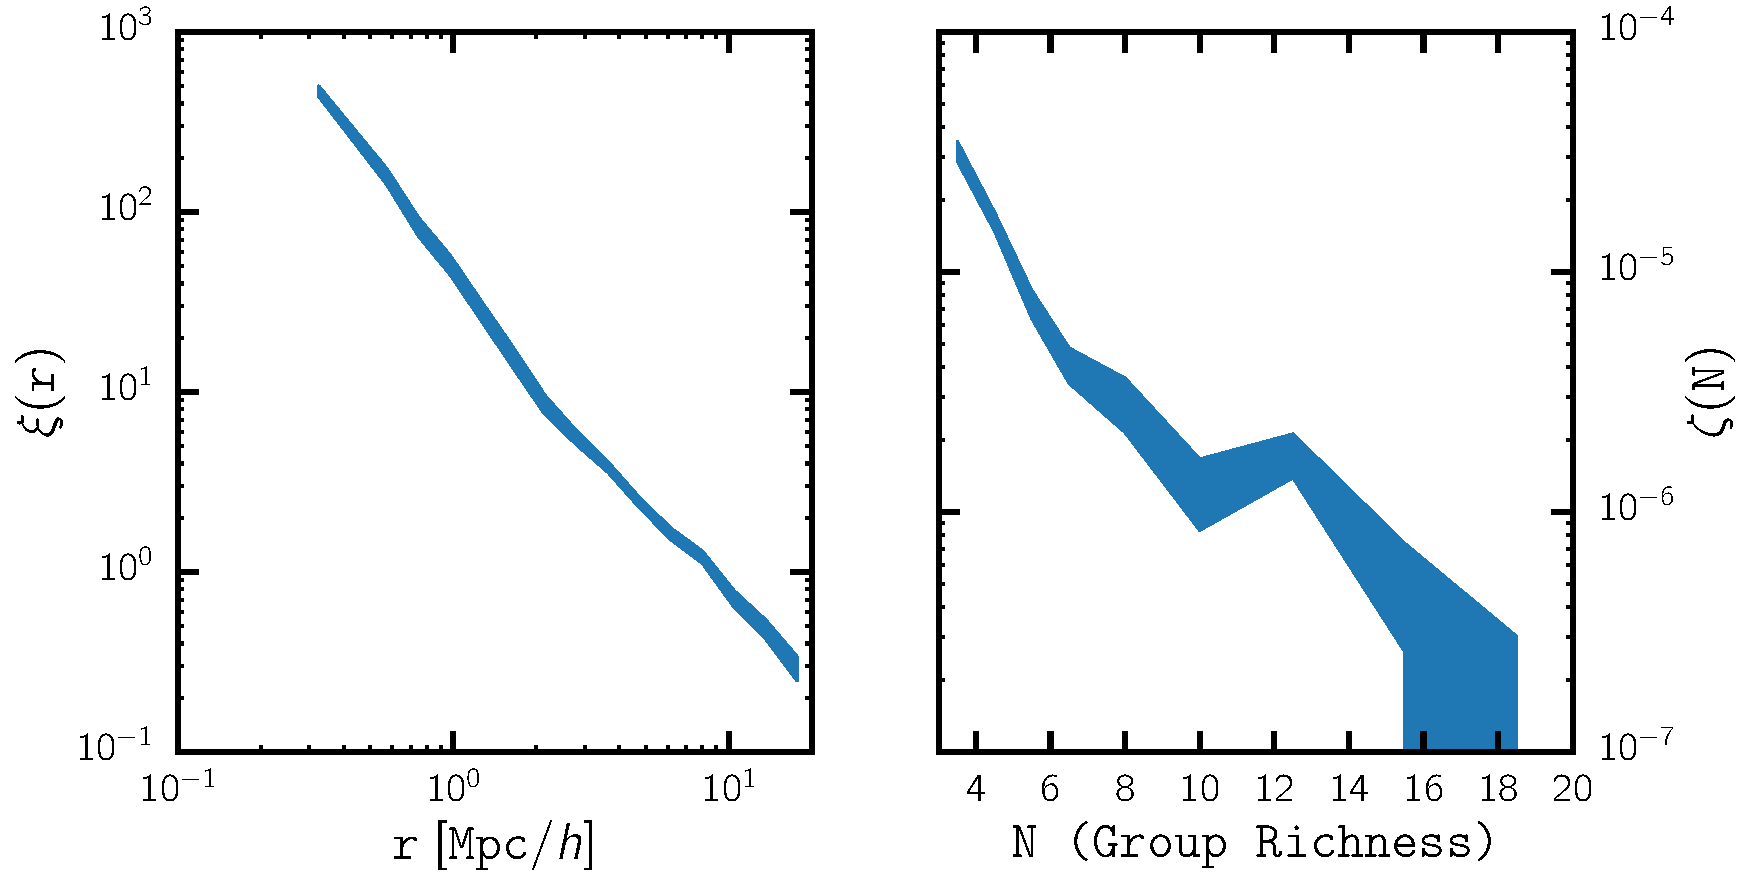
\includegraphics[width=\textwidth]{figures/abc/paper_data_observables.pdf}
\caption{\label{fig:mock} The two-point correlation function $\xigg(r)$ (left) and group multiplicity 
function $\gmf(N)$ (right) summary statistics of the mock observations generated from 
the ``true'' HOD parameters described in Section \ref{sec:mock_obv}. The width of the 
shaded region corresponds to the square root of the covariance matrix diagonal 
elements (Eq. \ref{eq:cov}). In our ABC analysis, we treat the $\xigg(r)$ 
and $\gmf(N)$ above as the summary statistics of the observation.}
%\end{center}
\end{figure*}

%%%%%%%%%%%%%%%%%%%%%%%%%%%%%%%%%%%%%%%%%%%%%%%%%%%%%%%%
% Figure: ABC Pool Evolution plot 
%%%%%%%%%%%%%%%%%%%%%%%%%%%%%%%%%%%%%%%%%%%%%%%%%%%%%%%%
\begin{figure*}
%\begin{center}
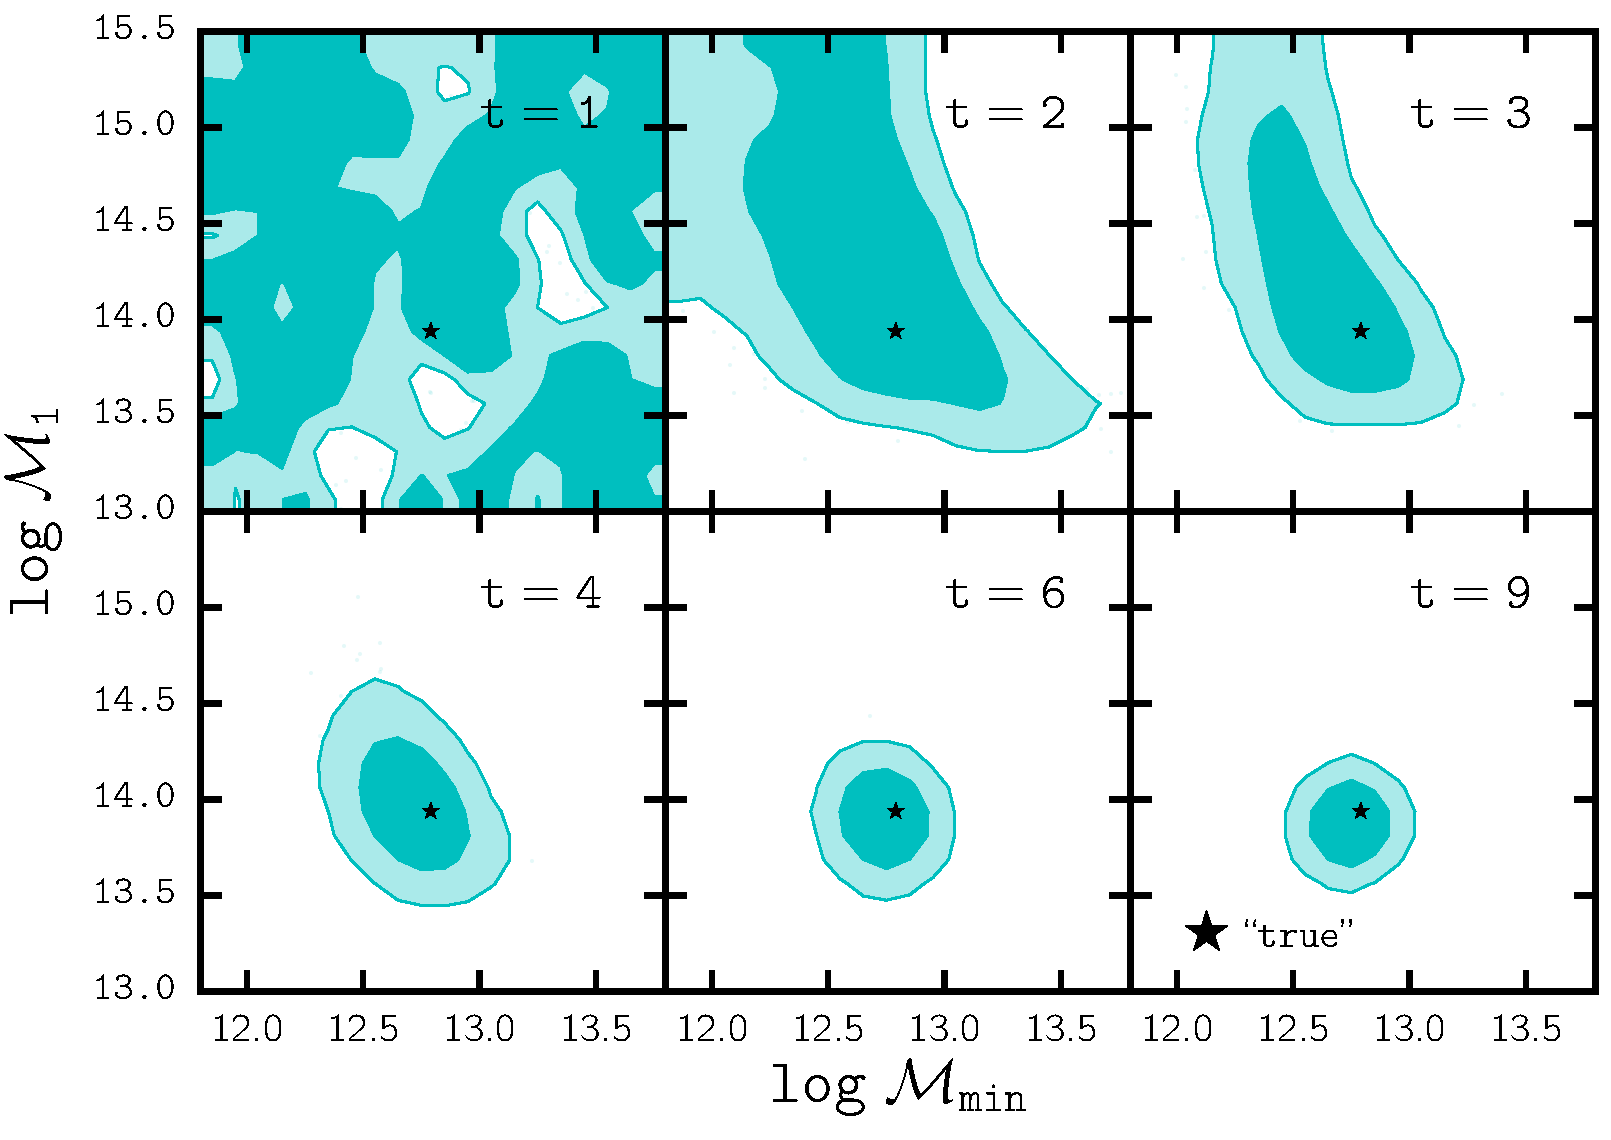
\includegraphics[width=0.8\textwidth]{figures/abc/paper_ABC_poolevolution_nbargmf.pdf}
\caption{\label{fig:pool_demo} We demonstrate the evolution of the ABC particles, $\pars_t$, over iterations $t = 1$ to $9$ in the $\log \mathcal{M}_{min}$ and $\log \mathcal{M}_1$ parameter space. 
$\bar{n}$ and $\gmf(N)$ are used as observables for the above results. For reference, 
in each panel, we include the ``true'' HOD parameters (black star) listed in 
Section \ref{sec:mock_obv}. The initial distance threshold, $\vec\epsilon_1 = 
[\infty, \infty]$ at $t=1$ (top left) so the $\pars_1$ spans the entire range of the prior distribution, 
which is also the range of the panels. We see for $t < 5$, the parameter space occupied 
by the ABC $\pars_t$ shrinks dramatically. Eventually when the algorithm converges, 
$t > 7$, the parameter space occupied by $\pars_t$ no longer shrinks and their 
distributions represent the posterior distribution of the 
parameters. At $t=9$, the final iteration, the ABC algorithm has converged and 
we find that $\pars_\mathrm{true}$ lies safely within the $68\%$ confidence region.} 
%\end{center}
\end{figure*}

%%%%%%%%%%%%%%%%%%%%% SECTION %%%%%%%%%%%%%%%%%%%%%%%%%%
%  ABC at work 
%%%%%%%%%%%%%%%%%%%%%%%%%%%%%%%%%%%%%%%%%%%%%%%%%%%%%%%%
\section{ABC at work}\label{sec:abcatwork}
With the methodology and the key components of ABC explained above, here we set out to 
demonstrate how ABC can be used to constrain HOD parameters. We start, in Section \ref{sec:mock_obv} 
by creating our ``observation''. We select a set of HOD parameters which we deem as the ``true'' 
parameters and run it through our forward model producing a catalog of galaxy positions 
which we treat as our observation. Then, in Section \ref{sec:abcpmc_spec}, we explain 
the distance metric and other specific choices we make for the ABC-PMC algorithm. 
Ultimately, we demonstrate the use of ABC in LSS, in Section \ref{sec:abc_results},
where we present the parameter constraints we get from our ABC analyses. 
Lastly, in order to both assess the quality of the ABC-PMC parameter inference and also 
discuss the assumptions of the standard Gaussian likelihood approach, we compare the 
ABC-PMC results to parameter constraints using the standard approach in Section 
\ref{sec:abcvsmcmc}.

%%%%%%%%%%%%%%%%%%%%% SUBSECTION %%%%%%%%%%%%%%%%%%%%%%%
% Mock Observations  
%%%%%%%%%%%%%%%%%%%%%%%%%%%%%%%%%%%%%%%%%%%%%%%%%%%%%%%%
\subsection{Mock Observations}\label{sec:mock_obv}
In generating our ``observations'', and more generally for our forward model, we adopt 
the HOD model from \cite{zheng07} where the expected number of galaxies populating a 
dark matter halo is governed by Eqs (\ref{eq:ncen}) and (\ref{eq:nsat}). For the parameters 
of the model used to generate the fiducial mock observations, we choose the \cite{zheng07} best-fit HOD parameters for the 
SDSS main galaxy sample with a luminosity threshold $M_{r} = -21$: 
\begin{center}
\renewcommand{\arraystretch}{1.5}
\begin{tabular}{ccccc} \hline \hline 
$\log M_{\rm min}$ & $\sigma_{\log M}$ & $\log M_{0}$ & $\log M_{1}$ & $\alpha$ \\ \hline
$12.79$ & $0.39$ & $11.92$ & $13.94$ & $1.15$ \\ \hline 
\end{tabular} \par
\end{center}
Since these parameters are used to generate the mock observation, they are the parameters
that we ultimately want to recover from our parameter inference. We refer to them as the
true HOD parameters. Plugging them into our forward model (Section \ref{sec:forwardmodel}), 
we generate a catalog of galaxy positions. 

For our summary statistics of the catalogs we use: 
the mean number density $\ngalaxy$, the galaxy two-point correlation function $\xigg(r)$, 
and the group multiplicity function $\gmf(N)$. Our mock observation catalog has 
$\ngalaxy = 9.28875 \times 10^{-4} \;h^{-3} \mathrm{Mpc}^3$ and in Figure \ref{fig:mock} 
we plot $\xigg(r)$ (left panel) and $\gmf(N)$ (right panel). The width of the shaded region
represent the square root of the diagonal elements of the summary statistic covariance matrix, 
which is computed as we describe below. 

We calculate $\xigg$ using the natural estimator (Section \ref{sec:statistics}) with 
fifteen radial bins. The edges of the first radial bin are $0.15$ and $0.5 \; 
h^{-1}\mathrm{Mpc}$. The bin edges for the next 14 bins are logarithmically-spaced between 
$0.5$ and $20\;h^{-1}\mathrm{Mpc}$. We compute the $\gmf(N)$ as described in Section
\ref{sec:statistics} with nine richness bins where the bin edges are logarithmically-spaced 
between $3$ and $20$. To calculate the covariance matrix, we first run the forward model 
using the true HOD parameters for all $125$ halo catalog subvolumes: 
$\{\mathtt{BOX1}, ..., \mathtt{BOX125}\}$. 
We compute the summary statistics of each subvolume galaxy sample $k$: 
\beq
\mathbf{x}^{(k)}=[\ngalaxy, \; \xigg, \; \gmf],
\eeq
Then we compute the covariance matrix as
\begin{eqnarray} 
\mathrm{C}^\mathrm{sample}_{i,j} &=& 
\frac{1}{N_{\mathrm{mocks}}-1}\sum_{k=1}^{N_{\mathrm{mocks}}} 
\Big[\mathbf{x}^{(k)}_{i}-\overline{\mathbf{x}}_{i}\Big]
\Big[\mathbf{x}^{(k)}_{j}-\overline{\mathbf{x}}_{j}\Big], \label{eq:cov} \\
\mathrm{where} \; \overline{\mathbf{x}}_{i} &=& 
\frac{1}{N_{\mathrm{mocks}}}\sum_{k=1}^{N_{\mathrm{mocks}}} \mathbf{x}^{(k)}_{i}.
\end{eqnarray}

Throughout our ABC-PMC analysis, we treat the $\ngalaxy$, $\xigg(r)$, and $\gmf(N)$ we describe in this 
section as if they were the summary statistics of actual observations. 
However, we benefit from the fact that these observables are generated from mock observations 
using the true HOD parameters of our choice: we can use the true HOD parameters to assess the 
quality of the parameter constraints we obtain from ABC-PMC. 

%%%%%%%%%%%%%%%%%%%%%%%%%%%%%%%%%%%%%%%%%%%%%%%%%%%%%%%%
% Figure: ABC Pool Convergence 
%%%%%%%%%%%%%%%%%%%%%%%%%%%%%%%%%%%%%%%%%%%%%%%%%%%%%%%%
\begin{figure*}
%\begin{center}
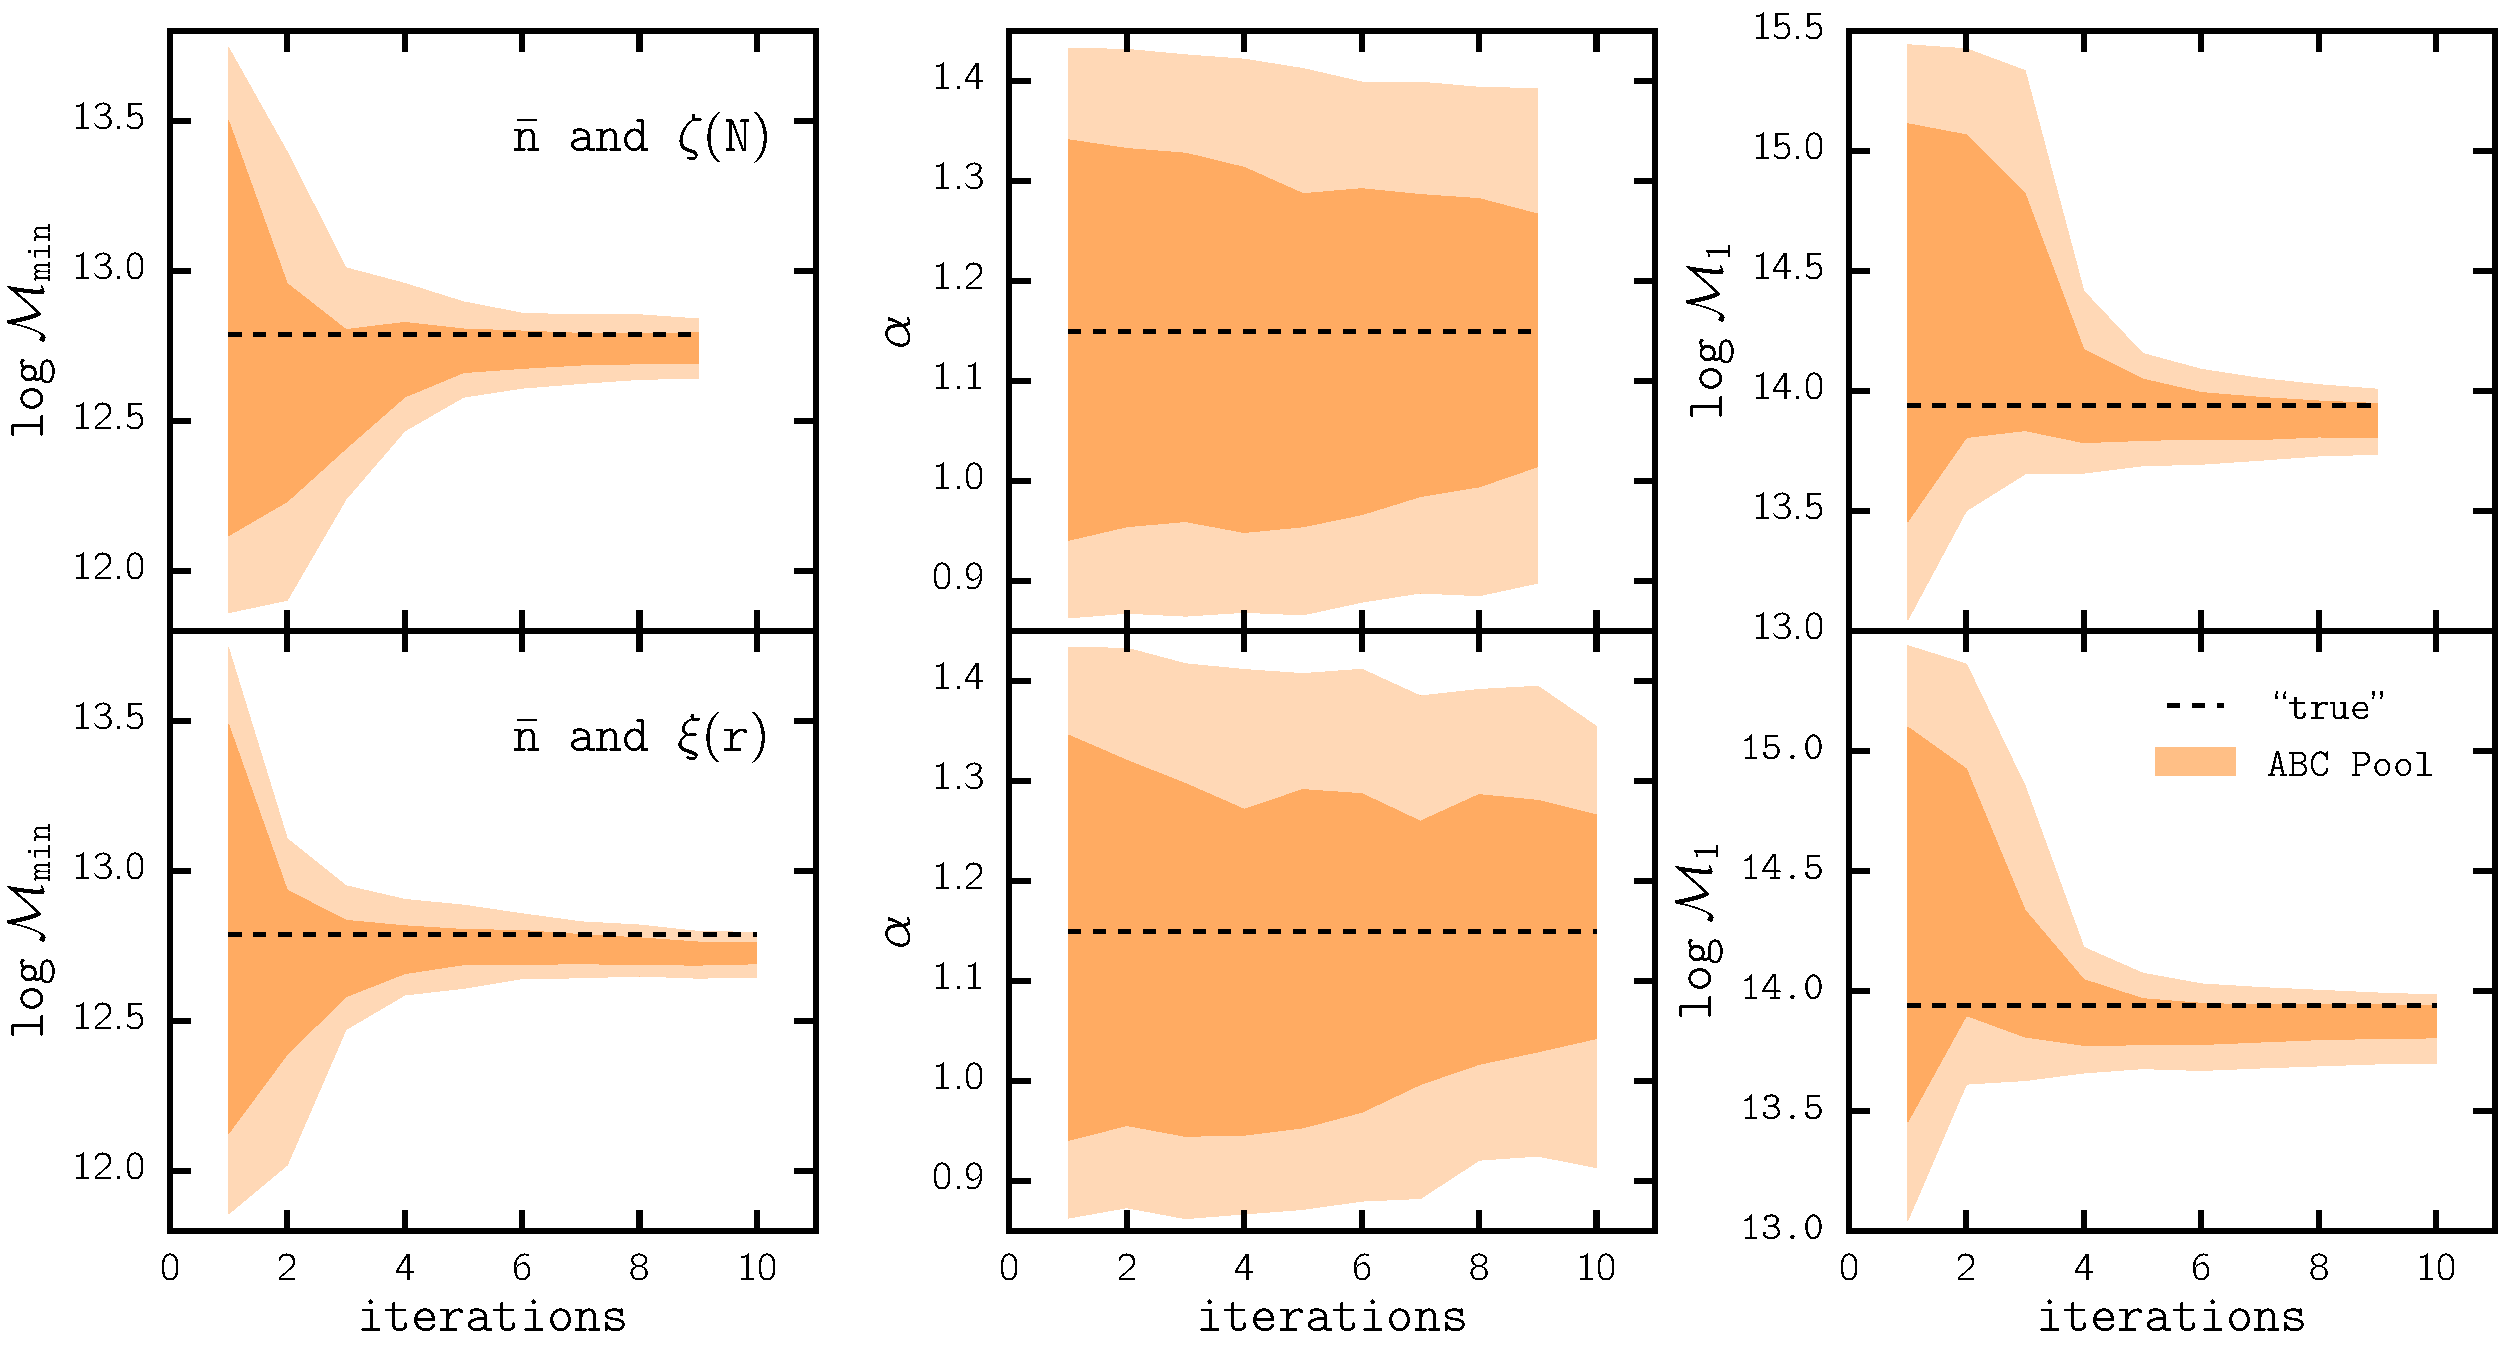
\includegraphics[width=\textwidth]{figures/abc/paper_ABCconvergence.pdf}
\caption{\label{fig:abc_converge} We illustrate the convergence of the ABC algorithm through the evolution of the ABC particle distribution as a function of iteration for 
parameters $\log \mathcal{M}_\mathrm{min}$ (left), $\alpha$ (center), and 
$\log \mathcal{M}_1$ (right).
The top panel corresponds our ABC results using the observables $(\bar{n}, \gmf(N))$, 
while the lower panel plots  corresponds to the ABC results using $(\bar{n}, \xigg(r))$. 
The distributions of parameters show no significant change after $t > 7$, which suggests
that the ABC algorithm has converged.}
%\end{center}
\end{figure*}

%%%%%%%%%%%%%%%%%%%%% SUBSECTION %%%%%%%%%%%%%%%%%%%%%%%
% ABC-PMC Design 
%%%%%%%%%%%%%%%%%%%%%%%%%%%%%%%%%%%%%%%%%%%%%%%%%%%%%%%%
\subsection{ABC-PMC Design} \label{sec:abcpmc_spec}
In Section \ref{sec:abc}, we describe the key components of the ABC algorithm we use in our analysis.
Now, we describe the more specific choices we make within the algorithm: the distance metric, 
the choice of priors, the distance threshold, and the convergence criteria. So far we have 
described three summary statistics: $\ngalaxy$, $\xigg(r)$, and $\gmf(N)$. In order to explore 
the detailed differences in the ABC-PMC parameter constraints based on our choice of summary 
statistics, we run our analysis for two sets of observables: ($\ngalaxy$, $\xigg$) and 
($\ngalaxy$, $\gmf$).

For both analyses, we use a multi-component distance (\citealt{silk12}, Cisewsky et al in preparation). 
Each summary statistic has a distance associated to it: $\rho_{n}$, $\rho_{\xi}$, and $\rho_{\zeta}$. 
We calculate each of these distance components as,   
\begin{eqnarray}
\rho_{n} &=& \frac{\left(\ngalaxy^\mathrm{d} - \ngalaxy^\mathrm{m} \right)^{2}}{\sigma^{2}_{n}}, \label{dn}\\
\rho_{\xi} &=& \sum_{k} \frac{\left[\xigg^\mathrm{d}(r_k) - \xigg^\mathrm{m}(r_k) \right]^{2}}{\sigma_{\xi,k}^{2}}, \label{dxi} \\
\rho_{\zeta} &=& \sum_{k} \frac{\left[\gmf^\mathrm{d}(N_k) - \gmf^\mathrm{m}(N_k) \right]^{2}}{\sigma_{\zeta,k}^{2}}. \label{dgmf}
\end{eqnarray}
The superscripts $\mathrm{d}$ and $\mathrm{m}$ denote the data and model respectively. The data, 
are the observables calculated from the mock observation (Section \ref{sec:mock_obv}). 
$\sigma_{n}^{2}$, $\sigma_{\xi,k}^{2}$, and $\sigma_{\zeta,k}^{2}$ are not the diagonal elements 
of the covariance matrix (\ref{eq:cov}). Instead, they are diagonal elements of the covariance matrix 
$C^\mathrm{ABC}$. 

We construct $C^\mathrm{ABC}$ by populating the entire $\mathtt{MultiDark}$ halo catalogs $125$ times 
repeatedly, calculating $\ngalaxy$, $\xigg$, and $\gmf$ for each realization, and then computing 
the covariance associated with these observables across all realizations. We highlight that $C^\mathrm{ABC}$ 
differs from Eq. \ref{eq:cov}, in that it does not populate the $125$ subvolumes but the entire 
$\mathtt{MultiDark}$ simulation and therefore does not incorporate sample variance. The ABC-PMC analysis 
instead accounts for the sample variance through the forward generative model, which populates the subvolumes
in the same manner as the observations. We use $\sigma_{n}^{2}$, $\sigma_{\xi,k}^{2}$, and $\sigma_{\zeta,k}^{2}$ 
to ensure that the distance is not biased to variations of observables on specific radial or richness bin. 

For our ABC-PMC analysis using the observables $\ngalaxy$ and $\xigg$, our distance metric 
$\vec\rho = [\rho_n, \rho_\xi]$ while the distance metric for the ABC-PMC analysis using 
the observables $\ngalaxy$ and $\gmf$, is $\vec\rho = [\rho_n, \rho_\zeta]$.
To avoid any complications from the choice for our prior, we select uniform priors over all parameters aside from the scatter parameter $\sigma_{\log\;M}$, for which we choose a log-uniform prior. 
We list the range of our prior distributions in Table ~\ref{tab:prior}.

With the distances and priors specified, we now describe the distance thresholds and the 
convergence criteria we impose in our analyses. For the initial iteration, we set distance
thresholds for each distance component to $\infty$. This means, that the initial pool 
$\vec\theta_1$ is simply sampled from the prior distribution we specify above. After the initial 
iteration, the distance threshold is adaptively lowered in subsequent iterations. More 
specifically, we follow the choice of \cite{abcwl} and set the distance threshold 
$\vec\epsilon_t$ to the median of $\vec\rho_{t-1}$, the multi-component distance of the 
previous iteration of particles ($\pars_{t-1}$).

The distance threshold $\vec\epsilon_t$ will progressively decrease. Eventually after a 
sufficient number of iterations, the region of parameter space occupied by $\pars_t$ 
will remain unchanged. As this happens, the acceptance ratio begins to fall significantly. 
When the acceptance ratio drops below $0.001$, our acceptance ratio threshold of choice, 
we deem the ABC-PMC algorithm as converged. In addition to the acceptance ratio threshold 
we impose, we also ensure that distribution of the parameters converges -- another sign 
that the algorithm has converged. Next, we present the results of our ABC-PMC analyses 
using the sets of observables ($\ngalaxy$, $\xigg$) and ($\ngalaxy$, $\gmf$). 

%%%%%%%%%%%%%%%%%%TABLES%%%%%%%%%%%%

\begin{table}
	\centering
	\caption{{\bf Prior Specifications}: The prior probability distribution 
  and its range for each of the \citet{zheng07} HOD parameters. All mass parameters are in unit of $\mstar$}
	\label{tab:prior}
	\begin{tabular}{lcr} % four columns, alignment for each
		\hline
		HOD Parameter & Prior & Range\\
		\hline
		$\alpha$ & Uniform & [0.8, 1.3]\\
		$\sigma_{\rm \log M}$ & Log-Uniform & [0.1, 0.7]\\
		$\log M_{0}$ & Uniform & [10.0, 13.0]\\
        $\log M_{min}$ & Uniform & [11.02, 13.02]\\
        $\log M_{1}$ & Uniform & [13.0, 14.0]\\
		\hline
	\end{tabular}
\end{table}

%%%%%%%%%%%%%%%%%%%%%%% SECTION: %%%%%%%%%%%%%%%%%%%%%%%
% SECTION: RESULTS 
%%%%%%%%%%%%%%%%%%%%%%%%%%%%%%%%%%%%%%%%%%%%%%%%%%%%%%%%
\subsection{Results: ABC}\label{sec:abc_results}
We describe the ABC algorithm in Section \ref{sec:abc} and list the particular choices
we make in the implementation in the previous section. Finally, we demonstrate how the 
ABC algorithm produces parameter constraints and present the results of our ABC analysis -- the 
parameter constraints for the \cite{zheng07} HOD model. 

We begin with a qualitative demonstration of the ABC algorithm in Figure \ref{fig:pool_demo},
where we plot the evolution of the ABC $\pars_t$ over the iterations $t = 1$ to $9$, 
in the parameter space of $[\log\mathcal{M}_1, \log\mathcal{M}_{min}]$. The ABC procedure we plot 
in Figure \ref{fig:pool_demo} uses $\bar{n}$ and $\gmf(N)$ for observables, but 
the overall evolution is the same when we use $\bar{n}$ and $\xigg(r)$. The darker and lighter 
contours represent the $68\%$ and $95\%$ confident regions of the posterior distribution over $\pars_t$. For reference, we also plot the ``true'' HOD parameter $\pars_\mathrm{true}$ 
(black star) in each of the panels.
The parameter ranges of the panels are equivalent to the ranges of the prior probabilities we 
specify in Table \ref{tab:prior}. 

For $t=1$, the initial pool (top left), the distance threshold $\vec\epsilon_1 = [\infty , \infty]$, 
so $\pars_1$ uniformly samples the prior probability over the parameters.
At each subsequent iteration, the threshold is lowered (Section \ref{sec:abcatwork}), so for 
$t < 6$ panels, we note that the parameter spaced occupied by $\pars_t$ dramatically shrinks. 
Eventually when the algorithm begins to converge, $t > 7$, the contours enclosing the $68\%$ and 
$95\%$ confidence interval stabilize. At the final iteration $t=9$ (bottom right), 
the algorithm has converged and we find that 
$\pars_\mathrm{true}$ lies within the $68\%$ confidence interval of the $\pars_{t=9}$ particle 
distribution. This $\pars_t$ distribution at the final iteration represents the 
posterior distribution of the parameters. 

To better illustrate the criteria for convergence, in Figure \ref{fig:abc_converge}, 
we plot the evolution of the $\pars_t$ distribution as a function of iteration 
for parameters $\log\mathcal{M}_\mathrm{min}$ (left), $\alpha$ (center), and 
$\log\mathcal{M}_1$ (right). The darker and lighter shaded regions correspond to the 
$68\%$ and $95\%$ confidence levels of the $\pars_t$ distributions. The top panels 
correspond to our ABC results using $(\bar{n}, \gmf)$ as observables and the bottom 
panels correspond to our results using $(\bar{n}, \xigg)$. 
For each of the parameters in both top and bottom panels, we find that the distribution 
does not evolve significantly for $t > 7$. At this point additional iterations in
our ABC algorithm will neither impact the distance threshold $\vec\epsilon_t$ nor 
the posterior distribution of $\pars_t$. We also emphasize that the convergence of the 
parameter distributions coincides with when the acceptance ratio, discussed in Section 
\ref{sec:abcpmc_spec}, crosses the predetermined shut-off value of $0.001$. Based on these criteria, 
our ABC results for both $(\bar{n}, \gmf)$ and $(\bar{n}, \xigg)$ observables have converged. 

We present the parameter constraints from the converged ABC analysis in Figure \ref{fig:abc_corner_nbarxi} and 
Figure \ref{fig:abc_corner_nbargmf}. Figure \ref{fig:abc_corner_nbarxi} shows 
the parameter constraints using $\bar{n}$ and $\xigg(r)$ while Figure 
\ref{fig:abc_corner_nbargmf} plots the constraints using $\bar{n}$ and $\gmf(N)$.
For both figures, the diagonal panels plot the posterior distribution of the 
HOD parameters with vertical dashed lines marking the $50\%$ (median) and $68\%$ 
confidence intervals. The off-diagonal panels plot the degeneracy between  
parameter pairs. To determine the accuracy of our ABC parameter constraints, we plot
the ``true'' HOD parameters (black) in each of the panels.
For both sets of observables, our ABC constraints are consistent with the 
``true'' HOD parameters. For $\log\mathcal{M}_0$, $\log\sigma_{\log M}$,
and $\alpha$, the true parameter values lie near the center of the $68\%$ confidence 
interval. For the other parameter, which have much tighter constraints, the true 
parameters lie within the $68\%$ confidence interval.  

To further test the ABC results, in Figure \ref{fig:abc_moneyplot}, 
we compare $\xigg(r)$ (left) and $\gmf(N)$ (right) of the mock observations from Section \ref{sec:mock_obv}
to the predictions of the ABC posterior distribution (shaded). The error bars of the mock observations 
represent the square root of the diagonal elements of the covariance matrix (Eq. \ref{eq:cov}) while the 
darker and lighter shaded regions represent the $68\%$ and $95\%$ confidence regions of the ABC posterior 
predictions. In the lower panels, we plot the ratio of the ABC posterior prediction $\xigg(r)$ and $\gmf(N)$ over
the mock observation $\xigg^\mathrm{obvs}(r)$ and $\gmf^\mathrm{obvs}(N)$. Overall, the 
ratio of the $68\%$ confidence region of ABC posterior predictions is consistent with unity 
throughout the $r$ and $N$ range. We observe slight deviations in the $\xigg$ ratio for 
$r > 5\;\mathrm{Mpc}/h$; however, any deviation is within the uncertainties of the mock observations. 
Therefore, the observables drawn from the ABC posterior distributions are in good agreement with the
observables of the mock observation. 

The ABC results we obtain using the algorithm of Section \ref{sec:abc} with the choices of
Section \ref{sec:abcpmc_spec} produce parameter constraints that are consistent with 
the ``true'' HOD parameters (Figures \ref{fig:abc_corner_nbarxi} and \ref{fig:abc_corner_nbargmf}).
They also produce observables $\xigg(r)$ and $\gmf(N)$ that are consistent with $\xigg^\mathrm{obvs}$ 
and $\gmf^\mathrm{obvs}$. Thus, through ABC we are able to produce consistent 
parameter constraints. {\em More importantly, we demonstrate that ABC is feasible 
for parameter inference in large scale structure.} % boom mic drop. 

%%%%%%%%%%%%%%%%%%%%%%% SECTION: %%%%%%%%%%%%%%%%%%%%%%%
% SECTION: Comparison to MCMC analysis  
%%%%%%%%%%%%%%%%%%%%%%%%%%%%%%%%%%%%%%%%%%%%%%%%%%%%%%%%
\subsection{Comparison to the Gaussian Pseudo-Likelihood MCMC Analysis} \label{sec:abcvsmcmc}
In order to assess the quality of the parameter inference described in the previous section, 
we compare the ABC-PMC results with the HOD parameter constraints from
assuming a Gaussian likelihood 
function. The model used for the Gaussian likelihood analysis is different than the forward 
generative model adopted for the ABC-PMC algorithm, to be consistent with the standard approach.

In the ABC analysis, the model accounts for sample variance by randomly sampling a subvolume to be 
populated with galaxies. Instead, in the Gaussian pseudo-likelihood analysis, the covariance matrix is assumed to capture the
uncertainties from sample variance. Hence, in the model for the Gaussian pseudo-likelihood analysis, 
we populate halos of the {\em entire} $\mathtt{MultiDark}$ simulation rather than a subvolume.
We describe the Gaussian pseudo-likelihood analysis below.

%The Gaussian likelihood analysis assumes a covariance matrix that captures the uncertainties from the sample variance, and therefore in the model, we populate the halos of the entire $\mathtt{MultiDark}$ simulation rather than a subvolume. 

To write down the Gaussian pseudo-likelihood, we first introduce the vector $\mathbf{x}$: 
a combination of the summary statistics (observables) for a galaxy catalog. 
When we use $\ngalaxy$ and $\xigg(r)$ as observables in the analysis: $\mathbf{x} = [\ngalaxy , \xigg]$;
when we use $\ngalaxy$ and $\gmf(N)$ as observables in the analysis: $\mathbf{x} = [\ngalaxy , \gmf]$.
Based on this notation, we can write pseudo-likelihood function as 
\begin{eqnarray}
-2 \ln \mathcal{L}(\theta | d) &=& \Delta \mathbf{x}^{T}\widehat{C^{-1}}\Delta \mathbf{x} + \ln\Big[(2\pi)^{d}\mathrm{det}(C)\Big], \label{loglike}
\end{eqnarray}
where 
\begin{eqnarray}
\Delta \mathbf{x} &=& [\mathbf{x}_{obs} -\mathbf{x}_{mod}], 
\end{eqnarray}
the difference between $\mathbf{x}_{obs}$, measured from the mock observation, 
and $\mathbf{x}_{mod}(\mathbb{\theta})$ measured from the mock catalog generated 
from the model with parameters $\theta$ .
$d$ here is the dimension of $\mathbf{x}$ (for $\mathbf{x} = [\ngalaxy, \xigg]$, $d = 13$; 
for $\mathbf{x} = [\ngalaxy, \gmf]$, $d = 10$).  
$\widehat{C^{-1}}$ is the inverse covariance matrix, which we estimate following \cite{hartlap2007}:
\begin{eqnarray}
\widehat{C^{-1}} = \frac{N_{\rm mocks}-d - 1}{N_{\rm mocks} -1} \; \widehat{C}^{-1}.
\end{eqnarray}
$\widehat{C}$ is the estimated covariance matrix, calculated using the corresponding 
$\mathbf{x}$ block of the covariance matrix from Eq.~\ref{eq:cov}, and $N_{\rm mock}$ 
is the number of mocks used for the estimation ($N_{\rm mock} = 124$; see Section \ref{sec:mock_obv}).
We note that in $\widehat{C}$ the dependence on the HOD parameters is neglected, 
so the second term in the expression of Eq.~\ref{loglike} can be neglected. 
Finally, using this pseudo-likelihood, we sample from the posterior distribution 
given the prior distribution using the MCMC sampler $\mathtt{emcee}$ (\citealt{emcee}). 

In Figures~\ref{fig:hist_nbarxi} and \ref{fig:hist_nbargmf}, we compare the results from
ABC-PMC and Gaussian pseudo-likelihood MCMC analyses using $[\ngalaxy, \xigg]$ and 
$[\ngalaxy, \gmf]$ as observables, respectively. The top panels in each figure 
compares the marginalized posterior PDFs for three parameters of the HOD model: 
$\{\log \mathcal{M}_{\rm min}, \alpha, \log\mathcal{M}_1\}$. The lower panels in each 
figure compares the $68\%$ and $95\%$ confidence intervals of the constraints 
derived from the two inference methods as a box plot. The ``true'' HOD parameters
are marked by vertical dashed lines in each panel. 



In both Figures~\ref{fig:hist_nbarxi} and \ref{fig:hist_nbargmf}, the marginalized 
posteriors for each of the parameters from both inference methods are comparable 
and consistent with the ``true'' HOD parameters. However, we note that there are 
minor discrepancies between the maringalized posterior distributions. In particular, 
the distribution for $\alpha$ derived from ABC-PMC is less biased than the $\alpha$ 
constraints from the Gaussian pseudo-likelihood approach. 

%The uncertainty over the parameter $\log \mathcal{M}_\mathrm{min}$ is slightly smaller while the uncertainties of the parameters $\alpha$ and $\log M_{1}$ are slightly larger for our ABC-PMC results.  In Figure \ref{fig:hist_nbargmf}, when we use $\ngalaxy$ and $\gmf$ as observables, both methods produce consistent constraints with each other and ``true'' HOD parameters. The lower panel of Figure \ref{fig:hist_nbargmf} shows that the uncertainties from the two methods are comparable. The ABC-PMC constraints over $\alpha$ is slightly less biased and slightly less precise. 


In Figures \ref{fig:cont_nbarxi} and \ref{fig:cont_nbargmf}, we plot the contours 
enclosing the $68\%$ and $95\%$ confidence regions of the posterior probabilities of 
the two methods using $[\ngalaxy, \xigg]$ and $[\ngalaxy, \gmf]$ as observables 
respectively. In both figures, we mark the ``true'' HOD parameters (black star). The 
overall shape of the contours are in agreement with each other. However, we note
that the contours for the ABC-PMC method are more extended along $\alpha$. 

%%% RefReport #1 
%%% CHH (3/8/2017): Made significant changes to the text in order to better emphasize
%%%      the advantages of ABC over MCMC

Overall, the HOD parameter constraints from ABC-PMC are consistent with those from 
the Gaussian pseudo-likelihood MCMC method; however, using ABC-PMC has a number of 
advantages. For instance, ABC-PMC utilizes a forward generative model. Our forward 
generative model accounts for sample variance. On the other hand, the Gaussian 
pseudo-likelihood approach, as mentioned earlier this section, does not account 
for sample variance in the model and relies on the covariance matrix estimate to 
capture the sample variance of the data. 


Accurate estimation of the covariance matrix 
in LSS, however, faces a number of challenges. It is both labor and computationally 
expensive and dependent on the accuracy of simulated mock catalogs, known to be 
unreliable on small scales~(see \citealt{cosmiccode,nifty} and references therein). 
In fact, as \cite{Sellentin:2016a} points out, using estimates of the covariance 
matrix in the Gaussian psuedo-likelihood approach become further problematic. Even 
when inferring parameters from a Gaussian-distributed data set, using covariance 
matrix estimates rather than the {\em true} covariance matrix leads to a likelihood 
function that is {\em no longer} Gaussian. ABC-PMC does not depend on a covariance 
matrix estimate; hence, it does not face these problems.


In addition to not requiring accurate covariance matrix estimates, forward models 
of the ABC-PMC method, in principle, also have the advantage that they can account 
for sources of systematic uncertainties that affect observations. All observations 
suffer from significant systematic effects which are often difficult to correct. 
For instance, in SDSS-III BOSS~\citep{boss}, fiber collisions and redshift
failures siginifcantly bias measurements and analysis of observables such as 
$\xigg$ or the galaxy powerspectrum~\citep{Ross:2012aa, Guo:2012a, Hahn:2017a}. 
In parameter inference, these systematics can affect the likelihood, and thus any 
analysis that requires writing down the likelihood, in unknown ways. With a forward generative model of the ABC-PMC 
method, the systematics can be simulated and marginalized out to achieve unbiased 
constraints. 

%{\bf \color{darkgreen} CHH: @MJV I incorporated the sentence into the paragraph. Can you check it out and confirm it's fine?  } 
%In general, we find that the constraints from ABC-PMC are consistent with those from the Gaussian-likelihood MCMC method both in terms of accuracy and precision. However, we emphasize some advantages of using ABC-PMC. ABC-PMC utilizes a forward generative model. Our forward generative model, for instance, accounts for sample variance. In principle, they also have the advantage that they can account for sources of systematic uncertainties in the observational data. 
%Furthermore, the Gaussian-likelihood  approach relies on constructing an accurate covariance matrix estimate that captures the sample variance of the data. While we are able to do this accurately within the scope of the HOD framework, for more general LSS parameter inference situations, it is both labor and computationally expensive and dependent on the accuracy of simulated mock catalogs, which are known to be unreliable on small scales (see \citealt{cosmiccode,nifty} and references therein).  Since ABC-PMC utilizes a forward model to account for sample variance, it does not depend on a covariance matrix estimate; hence it does not face these problems.  


Furthermore, {\em ABC-PMC -- unlike the Gaussian pseudo-likelihood approach -- 
is agnostic about the functional form of the underlying distribution of the 
summary statistics} (\emph{e.g.} $\xigg$ and $\gmf$). As we explain throughout 
the paper, the likelihood function in LSS {\em cannot} be Gaussian. For $\xigg$, 
the correlation function must satisfy non-trivial positive-definiteness requirements 
and hence the Gaussian pseudo-likelihood function assumption is not correct 
in detail. In the case of $\gmf(N)$, assuming a Gaussian functional form for 
the likelihood, which in reality is more likely Poisson, misrepresents the true 
likelihood function. In fact, this incorrect 
likelihood, may explain why the constraints on $\alpha$ are less biased for 
the ABC-PMC analysis than the Gaussian-likelihood analysis in \ref{fig:cont_nbargmf}.

%{\bf \color{darkgreen} CHH: @MJV, I parrot a lot of arguments made in the intro without providing much extra 'meat'. Let me know what you think.  }

Although in our comparison using simple mock observations, we find generally 
consistent parameter constraints from both the ABC-PMC analysis and the standard 
Gaussian pseudo-likelihood analysis, more realistic scenarios present many factors
that can generate inconsistencies. Consider a typical galaxy catalog from 
LSS observations. These catalogs consist of objects with different data 
qualities, signal-to-noise ratios, and systematic effects. For example, catalogs 
are often incomplete beyond some luminosity/redshift or have some threshold 
signal-to-noise ratio cut imposed on them.

%It is possible to consider a scenario in which the results from the standard analysis are inconsistent with the results from the ABC.  Let us consider a dataset---from a galaxy survey---consisting of objects with different data qualities, signal-to-noise ratios, and systematic effects.  This could be a catalog of galaxies which is incomplete beyond a certain luminosity or redshift. Another example could be a catalog with a signal-to-noise ratio cut.

These selection effects, coupled with the systematic effects earlier this section, 
make correctly predicting the likelihood intractable. In the standard Gaussian 
pseudo-likelihood analysis, and other analysis that require writing down a 
likelihood function, these effects can significantly 
bias the inferred parameter constraints. In these situations, employing
ABC equipped with a generative forward model that incorproates selection and 
systematic effects may produce less biased parameter constraints. 

%Methods that rely on a likelihood function may not correctly predict how the functional form of the likelihood is impacted by the presence of possible selection effects and systematic uncertainties.  
%Alternatively, one could alleviate this issue by employing ABC equipped with a generative forward model of the simulated data that incorporates signal-to-noise ratio cuts, incompleteness, systematic uncertainties etc. }{
%\bf \color{darkgreen} MJV: @CHH Can you read the two paragraphs above and see if they address referee's concern about the extreme data situation that could lead to discrepancy ? }
%%%
%In general, we find that the constraints from ABC-PMC are consistent with those from the Gaussian-likelihood 
%MCMC method both in terms of accuracy and precision. However, we emphasize some advantages of using 
%ABC-PMC. ABC-PMC utilizes a forward generative model. Our forward generative model, for instance, 
%accounts for sample variance. In principle, they also have the advantage that they can account for 
%sources of systematic uncertainties in the observational data. 

Despite the advantages of ABC, one obstactle for adopting it to parameter 
inference has been the computational costs of generative forward models, a 
key element of ABC. By combining ABC with the PMC sampling method, however, 
ABC-PMC efficiently converges to give reliable posterior parameter constraints. 
In fact, in our analysis, the total computational resources required for the 
ABC-PMC analysis were {\em comparable} to the computational resources used 
for the Gaussian pseudo-likelihood analysis with MCMC sampling.


Applying ABC-PMC beyond the analysis in this work, to broader LSS analyses 
imposes some caveats. In this work, we focus on the galaxy-halo connection, so
our generative forward model populates halos with galaxies. LSS analyses 
for inferring cosmological parameters would require generating halos by 
running cosmological simulations. The forward models also need to accurately 
model the observation systematic effects of the latest observations. Hence, 
accurate generative forward models in LSS analyses demand improvements in simulations 
and significant computational resources in order to infer unbiased parameter 
constraints. Recent cosmology simulations show promising improvements 
in both accuracy and speed~\citep[\emph{e.g.}][]{fastpm}. Such developements
will be crucial for applying ABC-PMC to broader LSS analyses and exploiting 
the significant advantages that ABC-PMC offers.


%the ABC method of parameter inference has often been viewed as computationally infeasible due to the fact that it necessitates a generative forward model for a large number of realizations. However, by combining ABC with the PMC sampling method, we have a method that efficiently converges to give us reliable posteriors of the model parameters. Furthermore, in our analysis, the computational resources required for the ABC-PMC inference were comparable to those used in achieving convergence in the MCMC Gaussian-Likelihood inference. This is excluding the typically computationally intensive step of calculating a covariance matrix estimate.  Therefore, we find that ABC-PMC offers a method for parameter inference in large scale structure studies with a number of advantages we describe above. 
%{\bf \color{darkgreen}
%\begin{itemize}
%\item distance metric 
%\item End with how there's still hope because there's developments in fast simulations
%\end{itemize}
%}

%%%%%%%%%%%%%%%%%%%%%%%%%%%%%%%%%%%%%%%%%%%%%%%%%%%%%%%%
% Summary and Conclusion  
%%%%%%%%%%%%%%%%%%%%%%%%%%%%%%%%%%%%%%%%%%%%%%%%%%%%%%%%
\section{Summary and Conclusion}\label{sec:discussion}

%Approximate Bayesian Computation, ABC, is a generative, simulation-based 
%inference that is guaranteed to deliver correct parameter estimation with 
%an appropriate set of summary statistics of the data is selected. 
Approximate Bayesian Computation, ABC, is a generative, simulation-based
inference that can deliver correct parameter estimation with
appropriate choices for its design.
It has the advantage over the standard approach in that it 
does not require explicit knowledge of the likelihood function. It only relies on the ability to simulate
the observed data, accounting for the uncertainties associated with observation and on specifying a metric 
for the distance between the observed data and simulation. When the specification of the likelihood function 
proves to be challenging or when the true underlying distribution of the observable is unknown, 
ABC provides a promising alternative for inference.

The standard approach to large scale structure studies relies on the assumption that the likelihood function 
for the observables -- often two-point correlation function -- given the model has a Gaussian functional form. 
In other words, it assumes that the statistical summaries are Gaussian distributed. In principle to rigorously 
test such an assumption, a large number of realistic simulations would need to be generated in order to examine 
the actual distribution of the observables. This process, however, is prohibitively---both labor and computationally 
---expensive. Therefore, our assumption of a Gaussian likelihood function remains largely unconfirmed and so 
unknown. Fortunately, the framework of ABC permits us to bypass any 
assumptions regarding the distribution of observables. Through ABC, we can provide constraints for our models without making the unexamined assumption of Gaussianity. 

With the ultimate goal of demonstrating that ABC is feasible for LSS studies, we use it to 
constrain parameters of the halo occupation distribution, which dictates the galaxy-halo connection. 
We begin by constructing a mock observation of galaxy distribution with a chosen set of ``true'' HOD model 
parameters. Then we attempt to constrain these parameters using ABC. More specifically, in this paper: 

\begin{itemize}
\item We provide an explanation of the ABC algorithm and present how Population Monte Carlo can be utilized 
to efficiently reach convergence and estimate the posterior distributions of model parameters. 
We use this ABC-PMC algorithm with a generative forward model built with $\mathtt{Halotools}$, a software 
package for creating catalogs of galaxy positions based on models of the galaxy-halo connection such as the HOD. 

\item We choose $\ngalaxy$, $\xigg$ and $\gmf$ as observables and summary statistics of the galaxy position catalogs. 
And for our ABC-PMC algorithm, we specify a multi-component distance metric, uniform priors, 
a median threshold implementation, and an acceptance rate-based convergence criterion.

\item From our specific ABC-PMC method, we obtain parameter constraints that are consistent with the ``true'' HOD parameters of our mock observations. Hence we demonstrate that ABC-PMC can be used for parameter inference in LSS studies. 

\item We compare our ABC-PMC parameter constraints to constraints using the standard Gaussian-likelihood
MCMC analysis. The constraints we get from both methods are comparable in accuracy and precision. However, 
for our analysis using $\ngalaxy$ and $\gmf$ in particular, we obtain less biased posterior distributions when
comparing to the ``true'' HOD parameters. 
\end{itemize}

Based on our results, we conclude that ABC-PMC is able to consistently infer parameters in the context
of LSS. We also find that the computation required for our ABC-PMC and standard Gaussian-likelihood 
analyses are comparable. Therefore, with the statistical advantages that ABC offers, we present ABC-PMC 
as an improved alternative for parameter inference. 


\section*{Acknowledgements}

We thank Jessie Cisewsky for reading and making valuable comments on the draft. We would also like to thank Michael R. Blanton, Jeremy R. Tinker, Uros Seljak, Layne Price, 
Boris Leidstadt, Alex Malz, Patrick McDonald, and Dan Foreman-Mackey for productive 
and insightful discussions. MV was supported by NSF grant AST-1517237. DWH was supported 
by NSF (grants IIS-1124794 and AST-1517237), NASA (grant NNX12AI50G), and the Moore-Sloan 
Data Science Environment at NYU. KW was supported by NSF grant AST-1211889. Computations 
were performed using computational resources at NYU-HPC. We thank Shenglong Wang, the 
administrator of NYU-HPC computational facility, for his consistent and continuous support 
throughout the development of this project. We would like to thank the organizers of 
the AstroHackWeek 2015 workshop (\url{http://astrohackweek.org/2015/}), 
since the direction and the scope of this investigation was ---to some degree--- initiated 
through discussions in this workshop. Throughout this investigation, we have made use of 
publicly available software packages $\mathtt{emcee}$ and $\mathtt{abcpmc}$. We have also used the publicly available python implementation of the FoF algorithm $\mathtt{pyfof}$ (\url{https://github.com/simongibbons/pyfof}).

%%%%%%%%%%%%%%%%%%%%%%%%%%%%%%%%%%%%%%%%%%%%%%%%%%

%%%%%%%%%%%%%%%%%%%% FIGURES %%%%%%%%%%%%%%%%%%

%%%%%%%%%%%%%%%%%%%%%%%%%%%%%%%%%%%%%%%%%%%%%%%%%%%%%%%%
% ABC Corner Plots
%%%%%%%%%%%%%%%%%%%%%%%%%%%%%%%%%%%%%%%%%%%%%%%%%%%%%%%%
\begin{figure*}
%\begin{center}
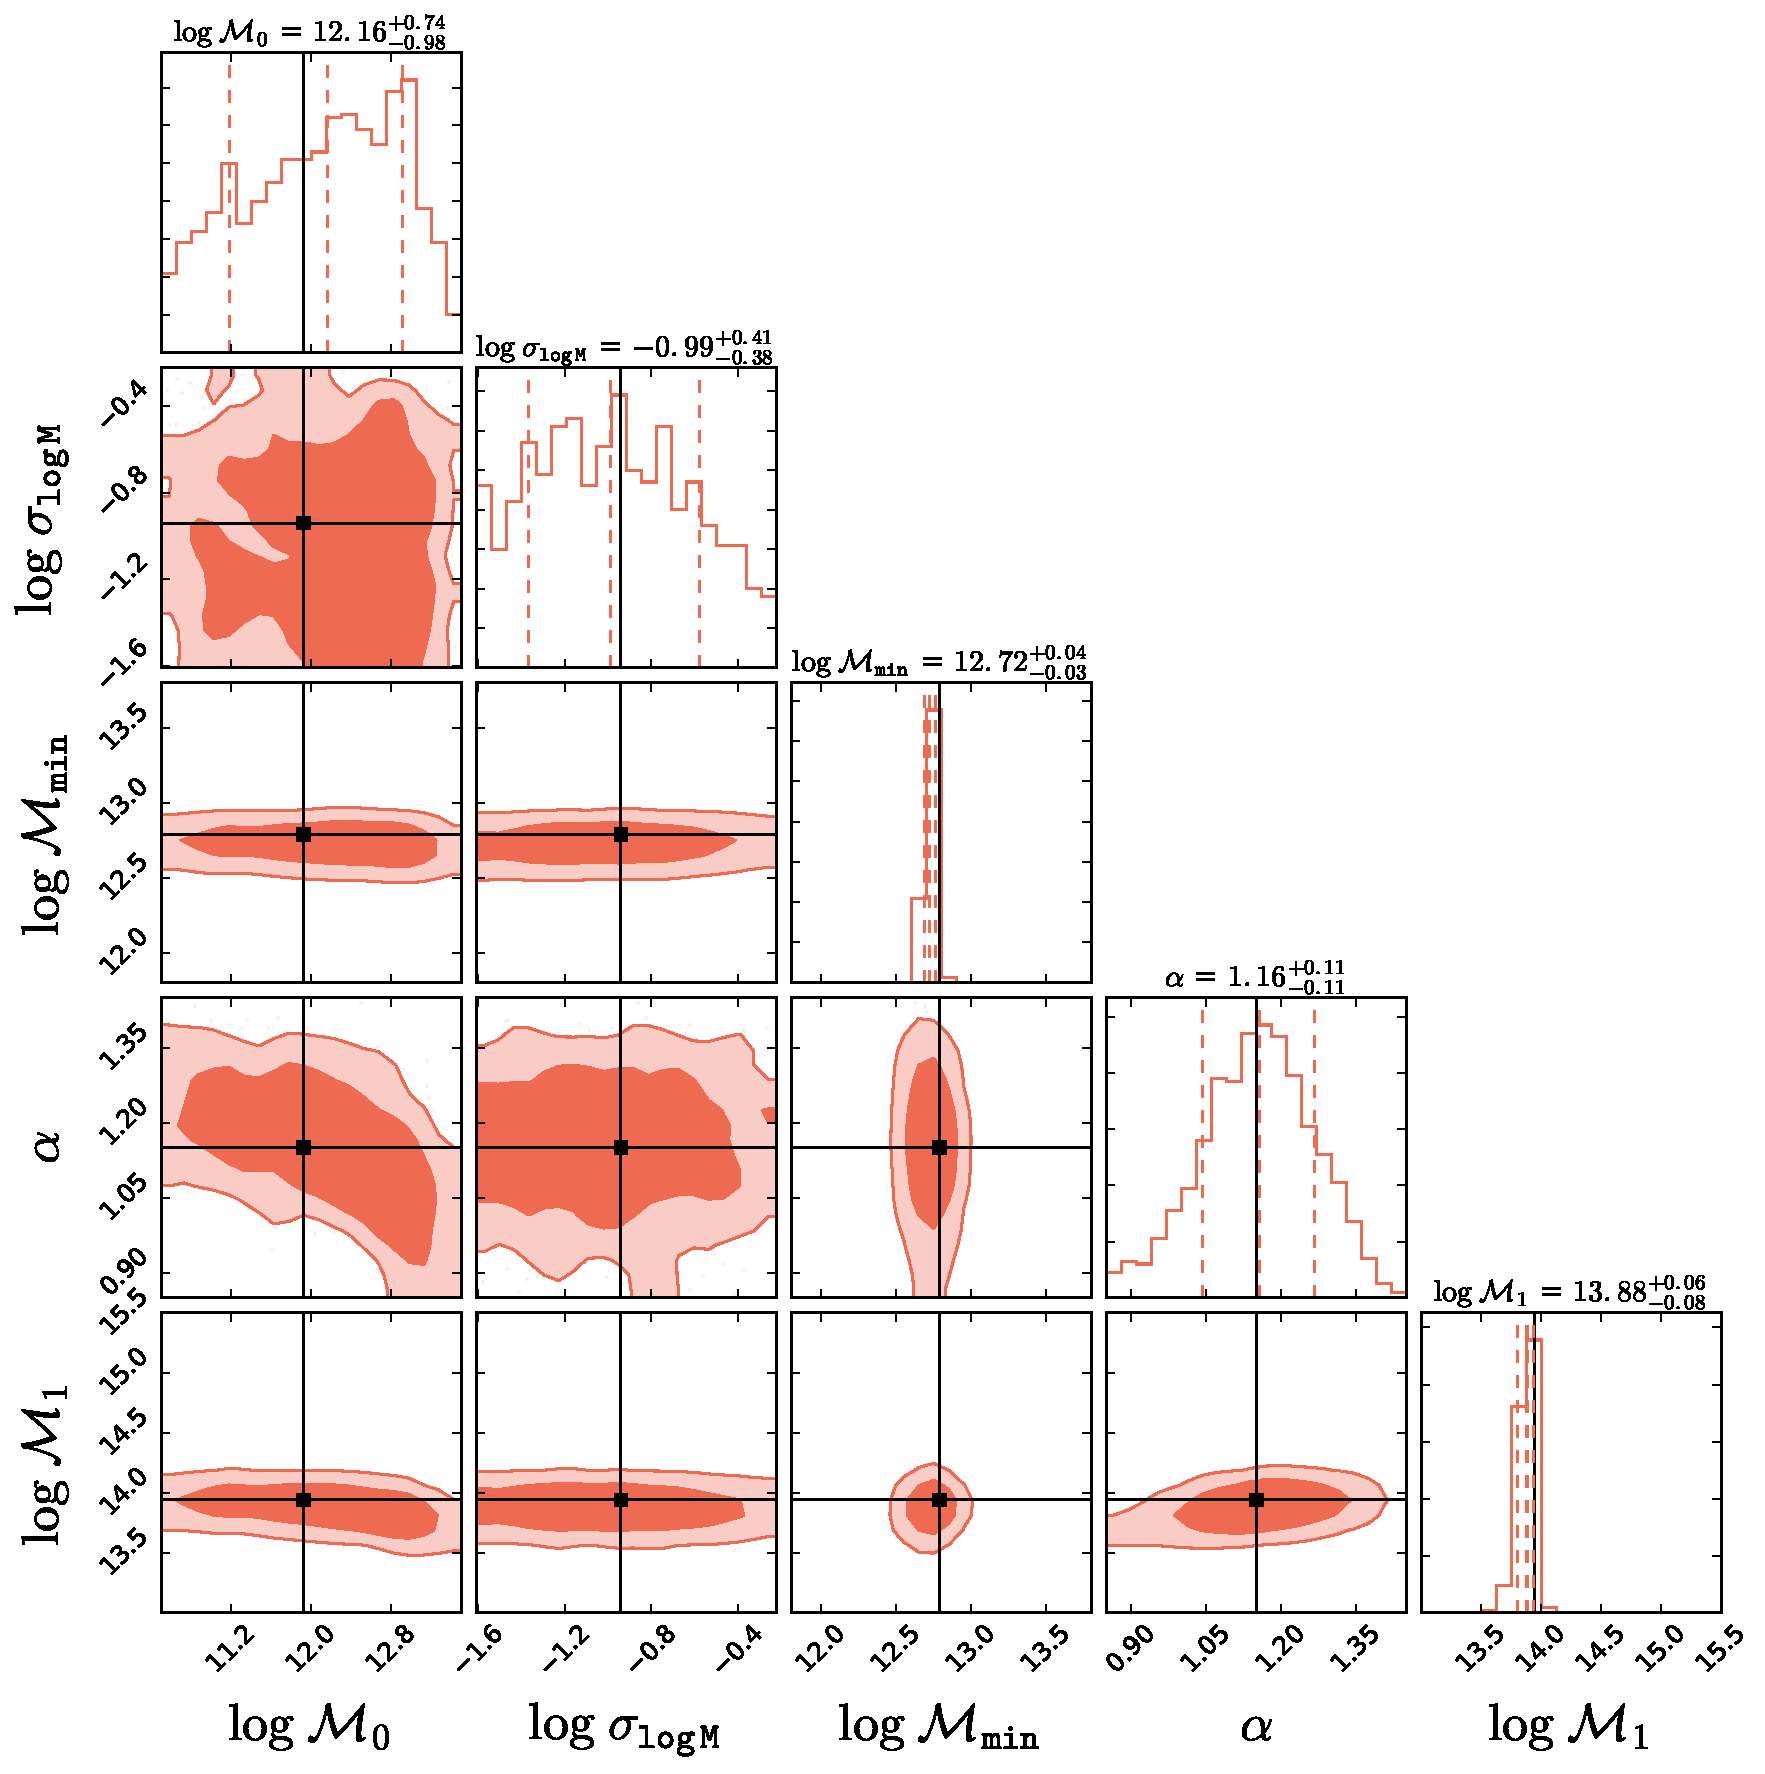
\includegraphics[width=0.85\textwidth]{figures/abc/paper_ABCcorner_nbarxi.pdf}
\caption{\label{fig:abc_corner_nbarxi} We present the constraints on the \citet{zheng07} HOD model parameters obtained from our ABC-PMC analysis using $\bar{n}$ and $\xigg(r)$ as observables.  
The diagonal panels plot the posterior distribution of each HOD parameter with 
vertical dashed lines marking the $50\%$ quantile and $68\%$ confidence intervals of the 
distribution. The off-diagonal panels plot the degeneracies between parameter pairs. 
The range of each panel corresponds to the range of our prior choice. The ``true''
HOD parameters, listed in Section \ref{sec:mock_obv}, are also plotted in each of 
the panels (black). For $\log\mathcal{M}_0$, $\alpha$, and $\sigma_{\log M}$, 
the ``true'' parameter values lie near the center of the $68\%$ confidence interval 
of the posterior distribution. For $\log\mathcal{M}_1$ and $\log\mathcal{M}_\mathrm{min}$, 
which have tight constraints, the ``true'' values lie within the $68\%$ confidence 
interval. Ultimately, the ABC parameter constraints we obtain in our analysis are consistent with the ``true'' HOD parameters.}
%\end{center}
\end{figure*}

\begin{figure*}
%\begin{center}
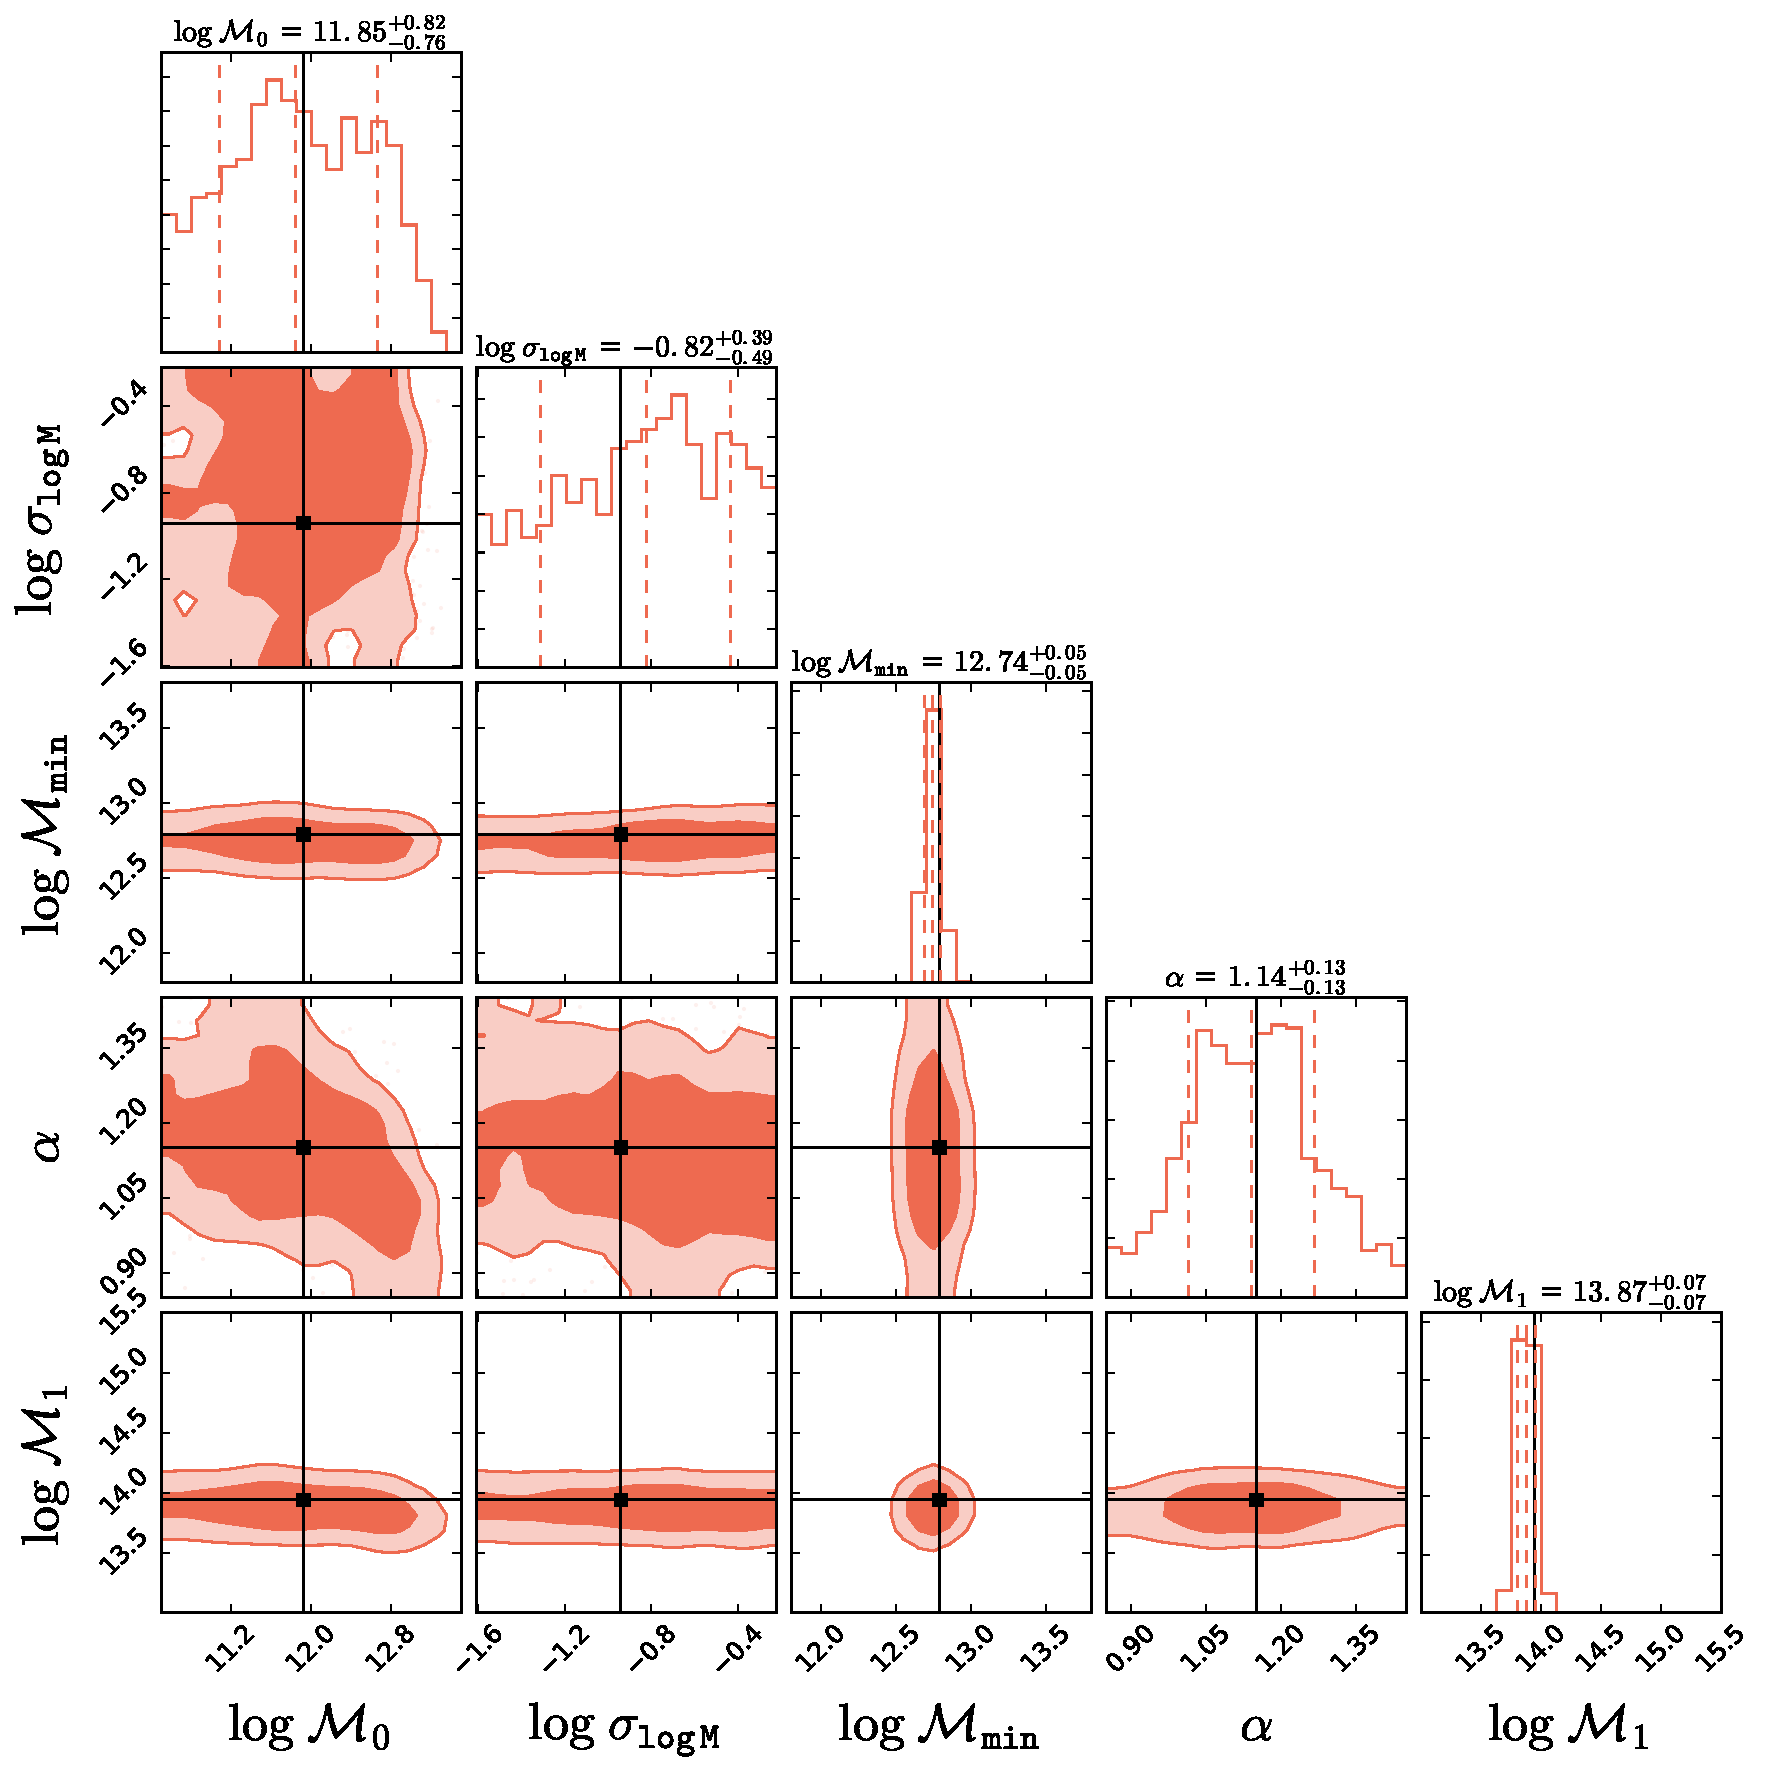
\includegraphics[width=0.85\textwidth]{figures/abc/paper_ABCcorner_nbargmf.pdf}
\caption{\label{fig:abc_corner_nbargmf}Same as Figure \ref{fig:abc_corner_nbarxi} but for our ABC analysis using $\bar{n}$ and $\gmf(N)$ as observables. The ABC parameter constraints we obtain are
consistent with the ``true'' HOD parameters.}
%\end{center}
\end{figure*}

%%%%%%%%%%%%%%%%%%%%%%%%%%%%%%%%%%%%%%%%%%%%%%%%%%%%%%%%
% ABC Posterior Observable  
%%%%%%%%%%%%%%%%%%%%%%%%%%%%%%%%%%%%%%%%%%%%%%%%%%%%%%%%
\begin{figure*}
%\begin{center}
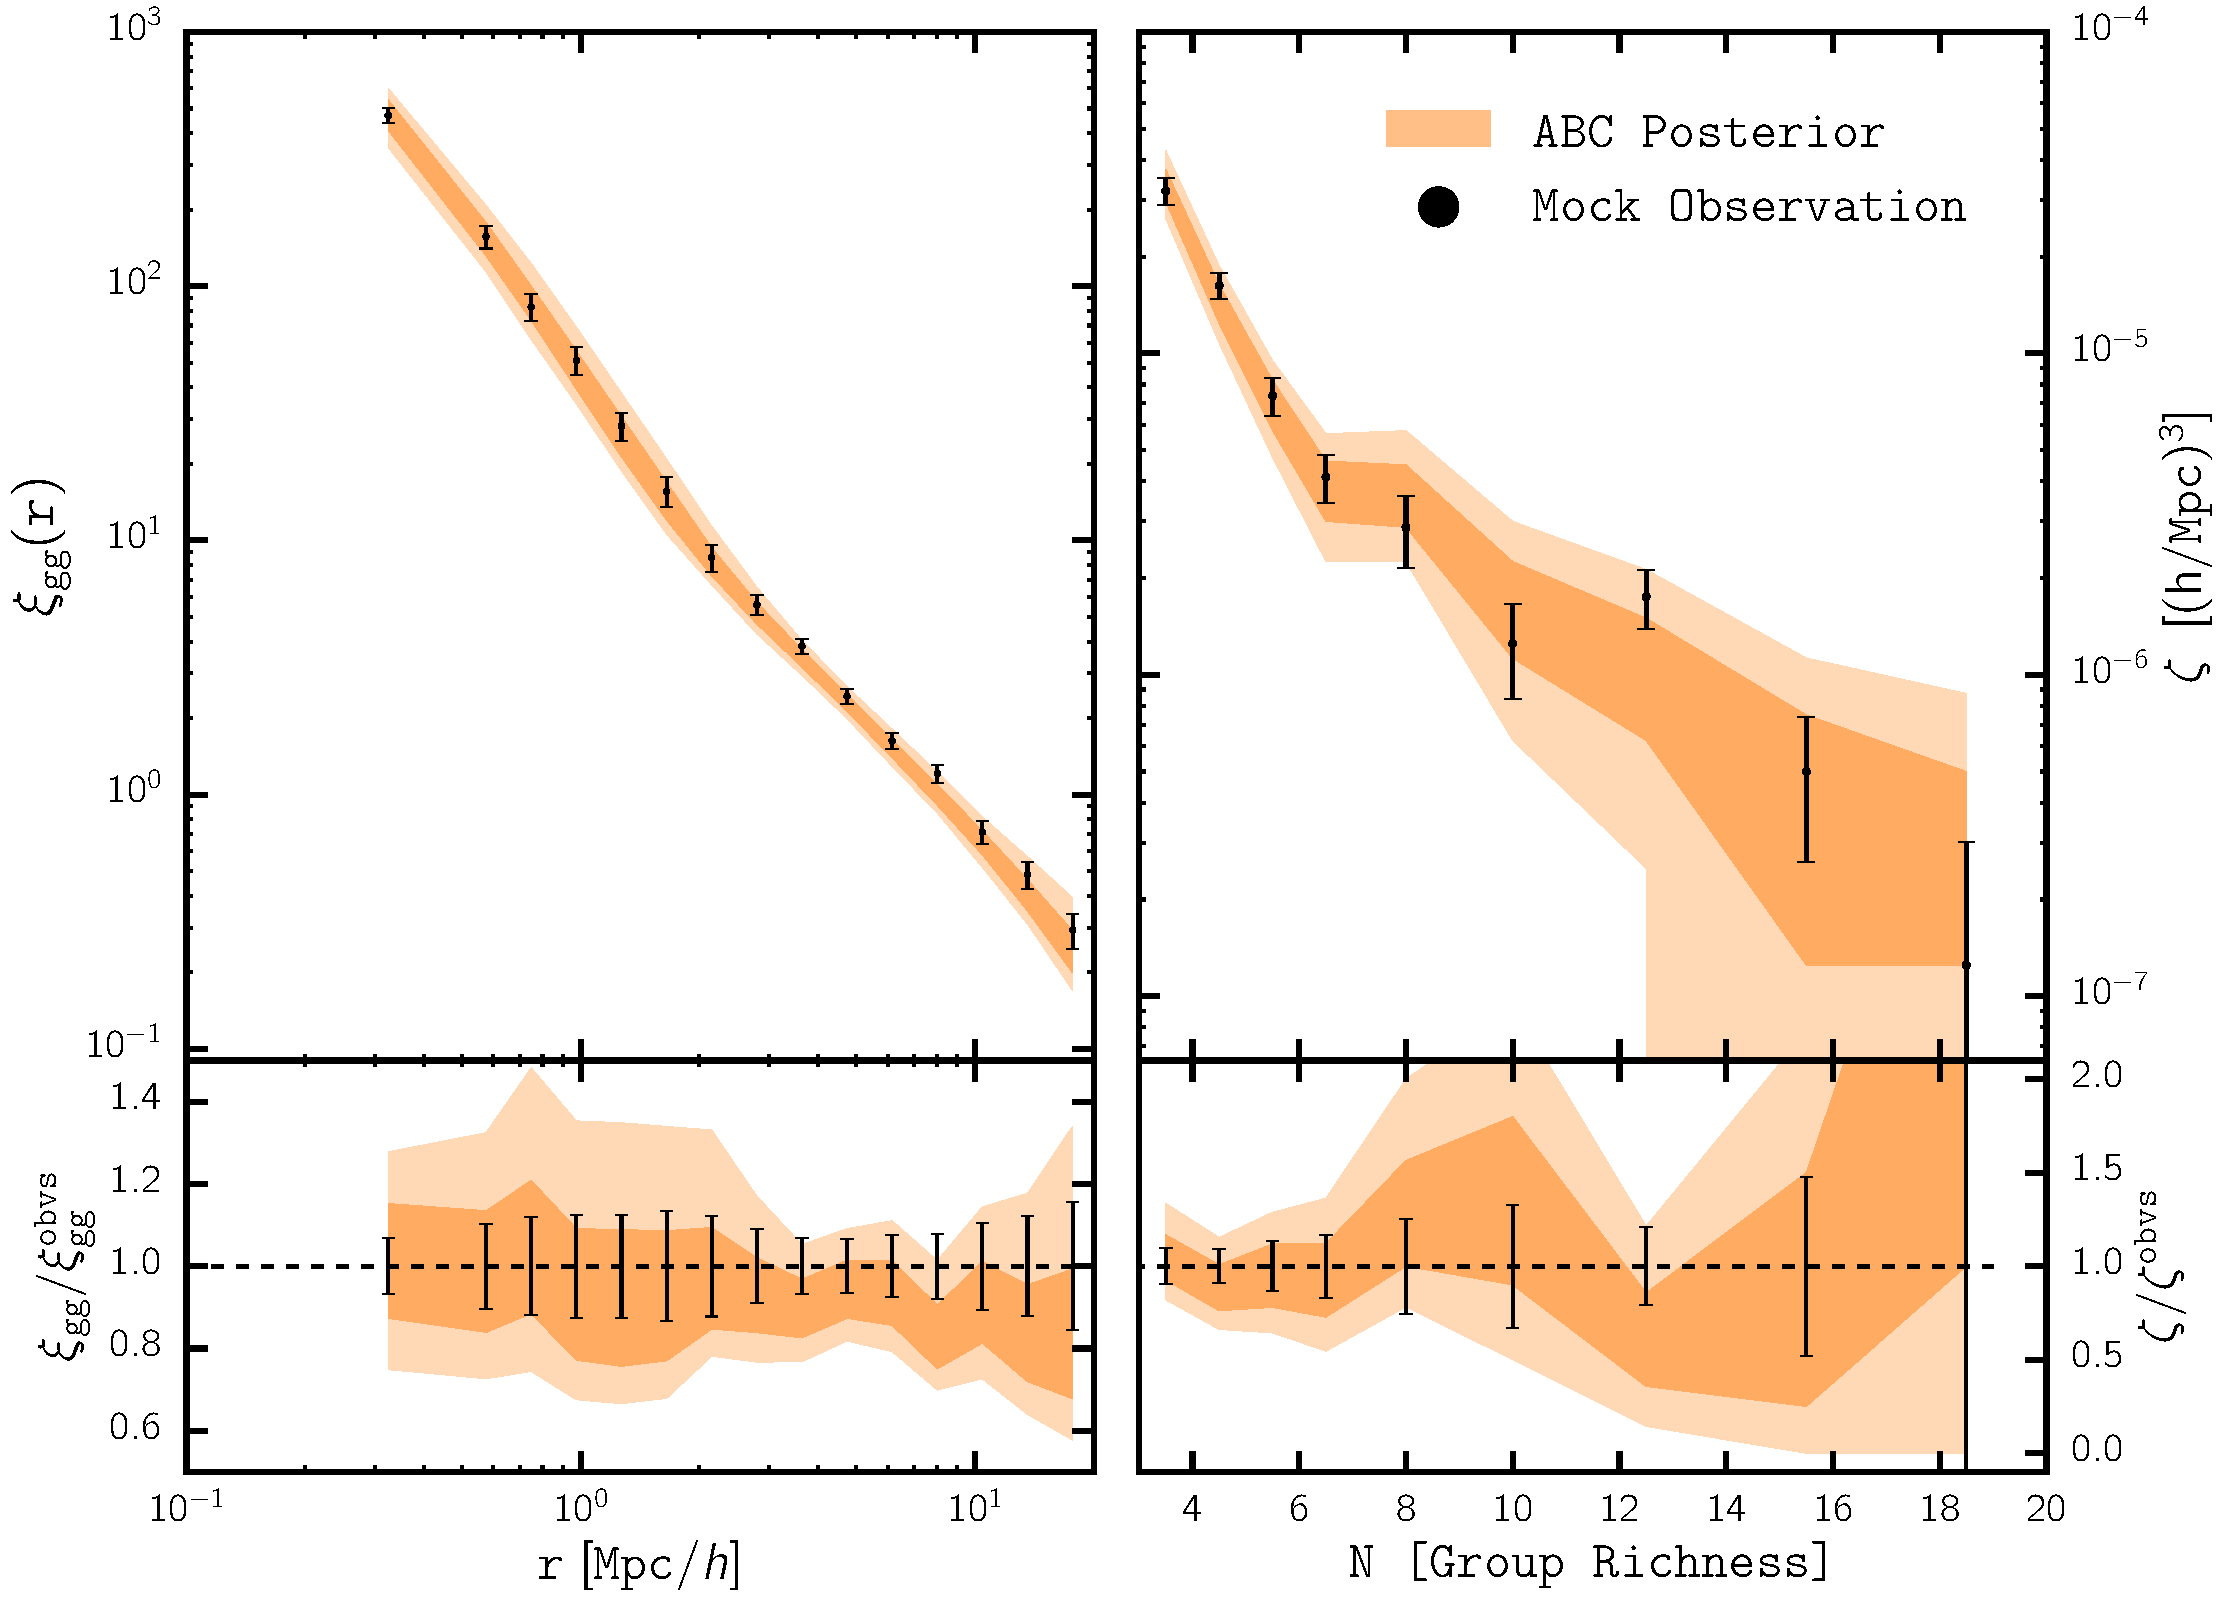
\includegraphics[width=\textwidth]{figures/abc/paper_ABCposterior.pdf}
\caption{\label{fig:abc_moneyplot} We compare the ABC-PMC posterior prediction for the observables $\xigg(r)$ (left) and $\gmf(N)$ (right) (orange; Section \ref{sec:abc_results}) 
to $\xigg(r)$ and $\gmf(N)$ of the mock observation (black) in the top panels.
In the lower panels, we plot the ratio between the ABC-PMC posterior predictions for $\xigg$ and $\gmf$ 
to the mock observation $\xigg^\mathrm{obvs}$ and $\gmf^\mathrm{obvs}$. The darker 
and lighter shaded regions represent the $68\%$ and $95\%$ confidence regions of the posterior predictions, 
respectively. The error-bars represent the square root of the diagonal elements of the error 
covariance matrix (equation \ref{eq:cov}) of the mock observations. Overall, the observables 
drawn from the ABC-PMC posteriors are in good agreement with $\xigg$ and $\gmf$ of the 
mock observations. The lower panels demonstrate that for both observables, the error-bars 
of the mock observations lie within the $68\%$ confidence interval of the ABC-PMC posterior 
predictions.} 
%\end{center}
\end{figure*}

%%%%%%%%%%%%%%%%%%%%%%%%%%%%%%%%%%%%%%%%%%%%%%%%%%%%%%%%
% ABC vs MCMC Histograms 
%%%%%%%%%%%%%%%%%%%%%%%%%%%%%%%%%%%%%%%%%%%%%%%%%%%%%%%%
\begin{figure*}
%\begin{center}
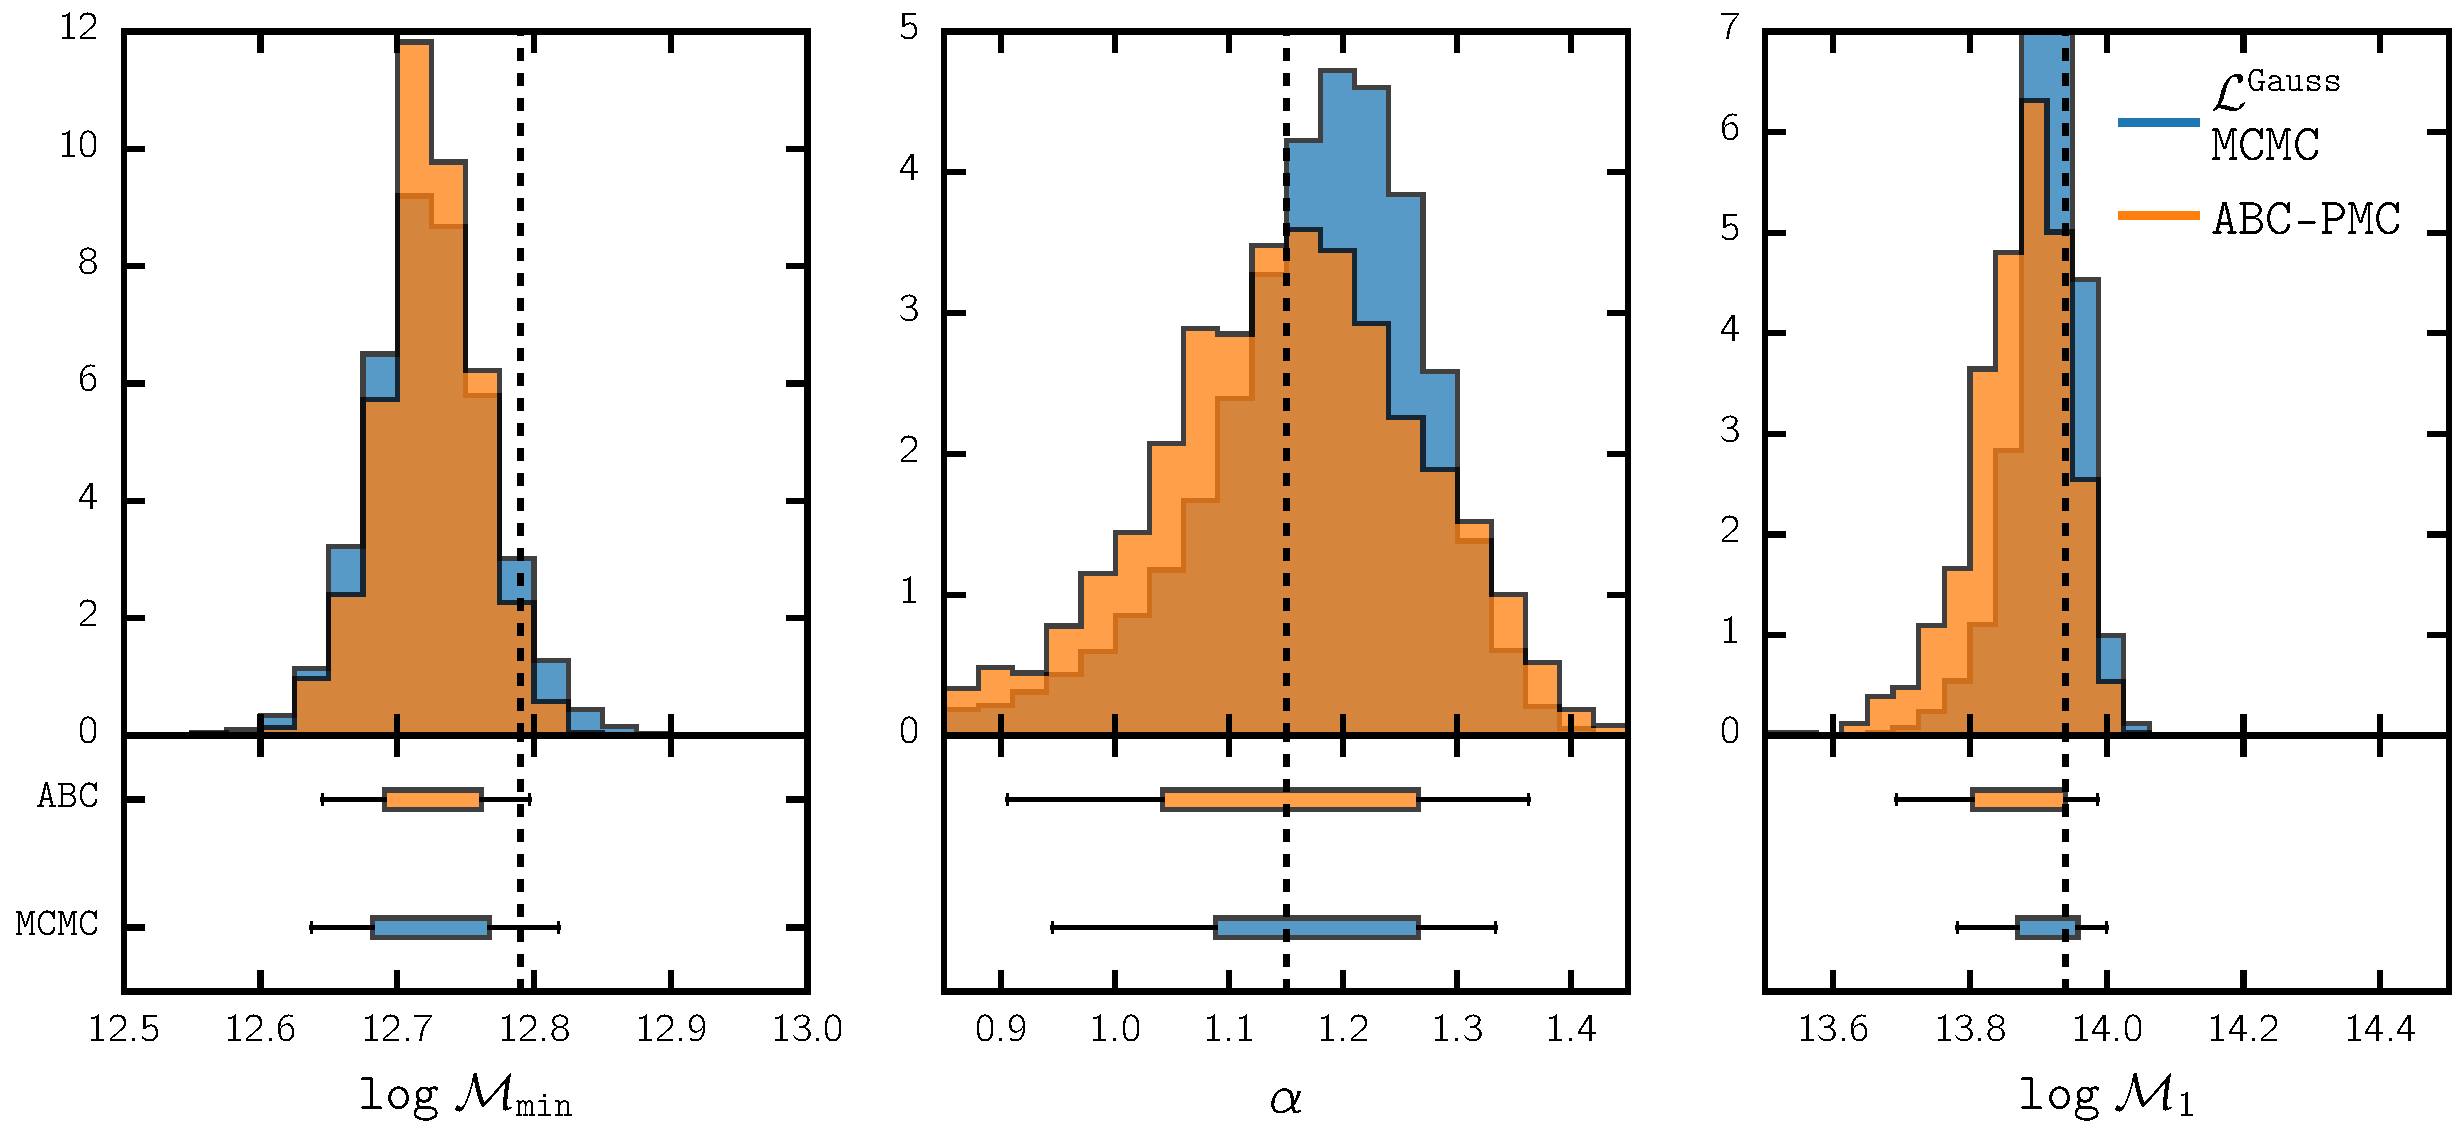
\includegraphics[width=1.\textwidth]{figures/abc/paper_ABCvsMCMC_nbarxi.pdf}
\caption{\label{fig:hist_nbarxi} 
We compare the $\log \mathcal{M}_{\rm min}$, $\alpha$, and $\log \mathcal{M}_{1}$ parameter 
constraints from ABC-PMC (orange) to constraints from the Gaussian pseudo-ikelihood MCMC (blue) 
using $\ngalaxy$ and $\xigg(r)$ as observables. The \emph{top} panels compares the two methods' 
marginalized posterior PDFs over the parameters. In the \emph{bottom} panels, we include box 
plots marking the confidence intervals of the posterior distributions. The boxes represent the 
$68\%$ confidence interval while the ``whiskers'' represent the $95\%$ confidence interval. We mark 
the ``true'' HOD parameters with vertical black dashed line. The marginalized posterior PDFs 
obtained from the two methods are consistent with each other. The ABC-PMC and Gaussian pseudo-likelihood
constraints are generally consistent for $\log \mathcal{M}_{\rm min}$ and $\log \mathcal{M}_{1}$. 
The ABC-PMC constraint for $\alpha$ is slightly less biased and has slightly larger uncertainty
then the constraint from Gaussian pseudo-likelihood analysis.} 
%\end{center}
\end{figure*}

\begin{figure*}
%\begin{center}
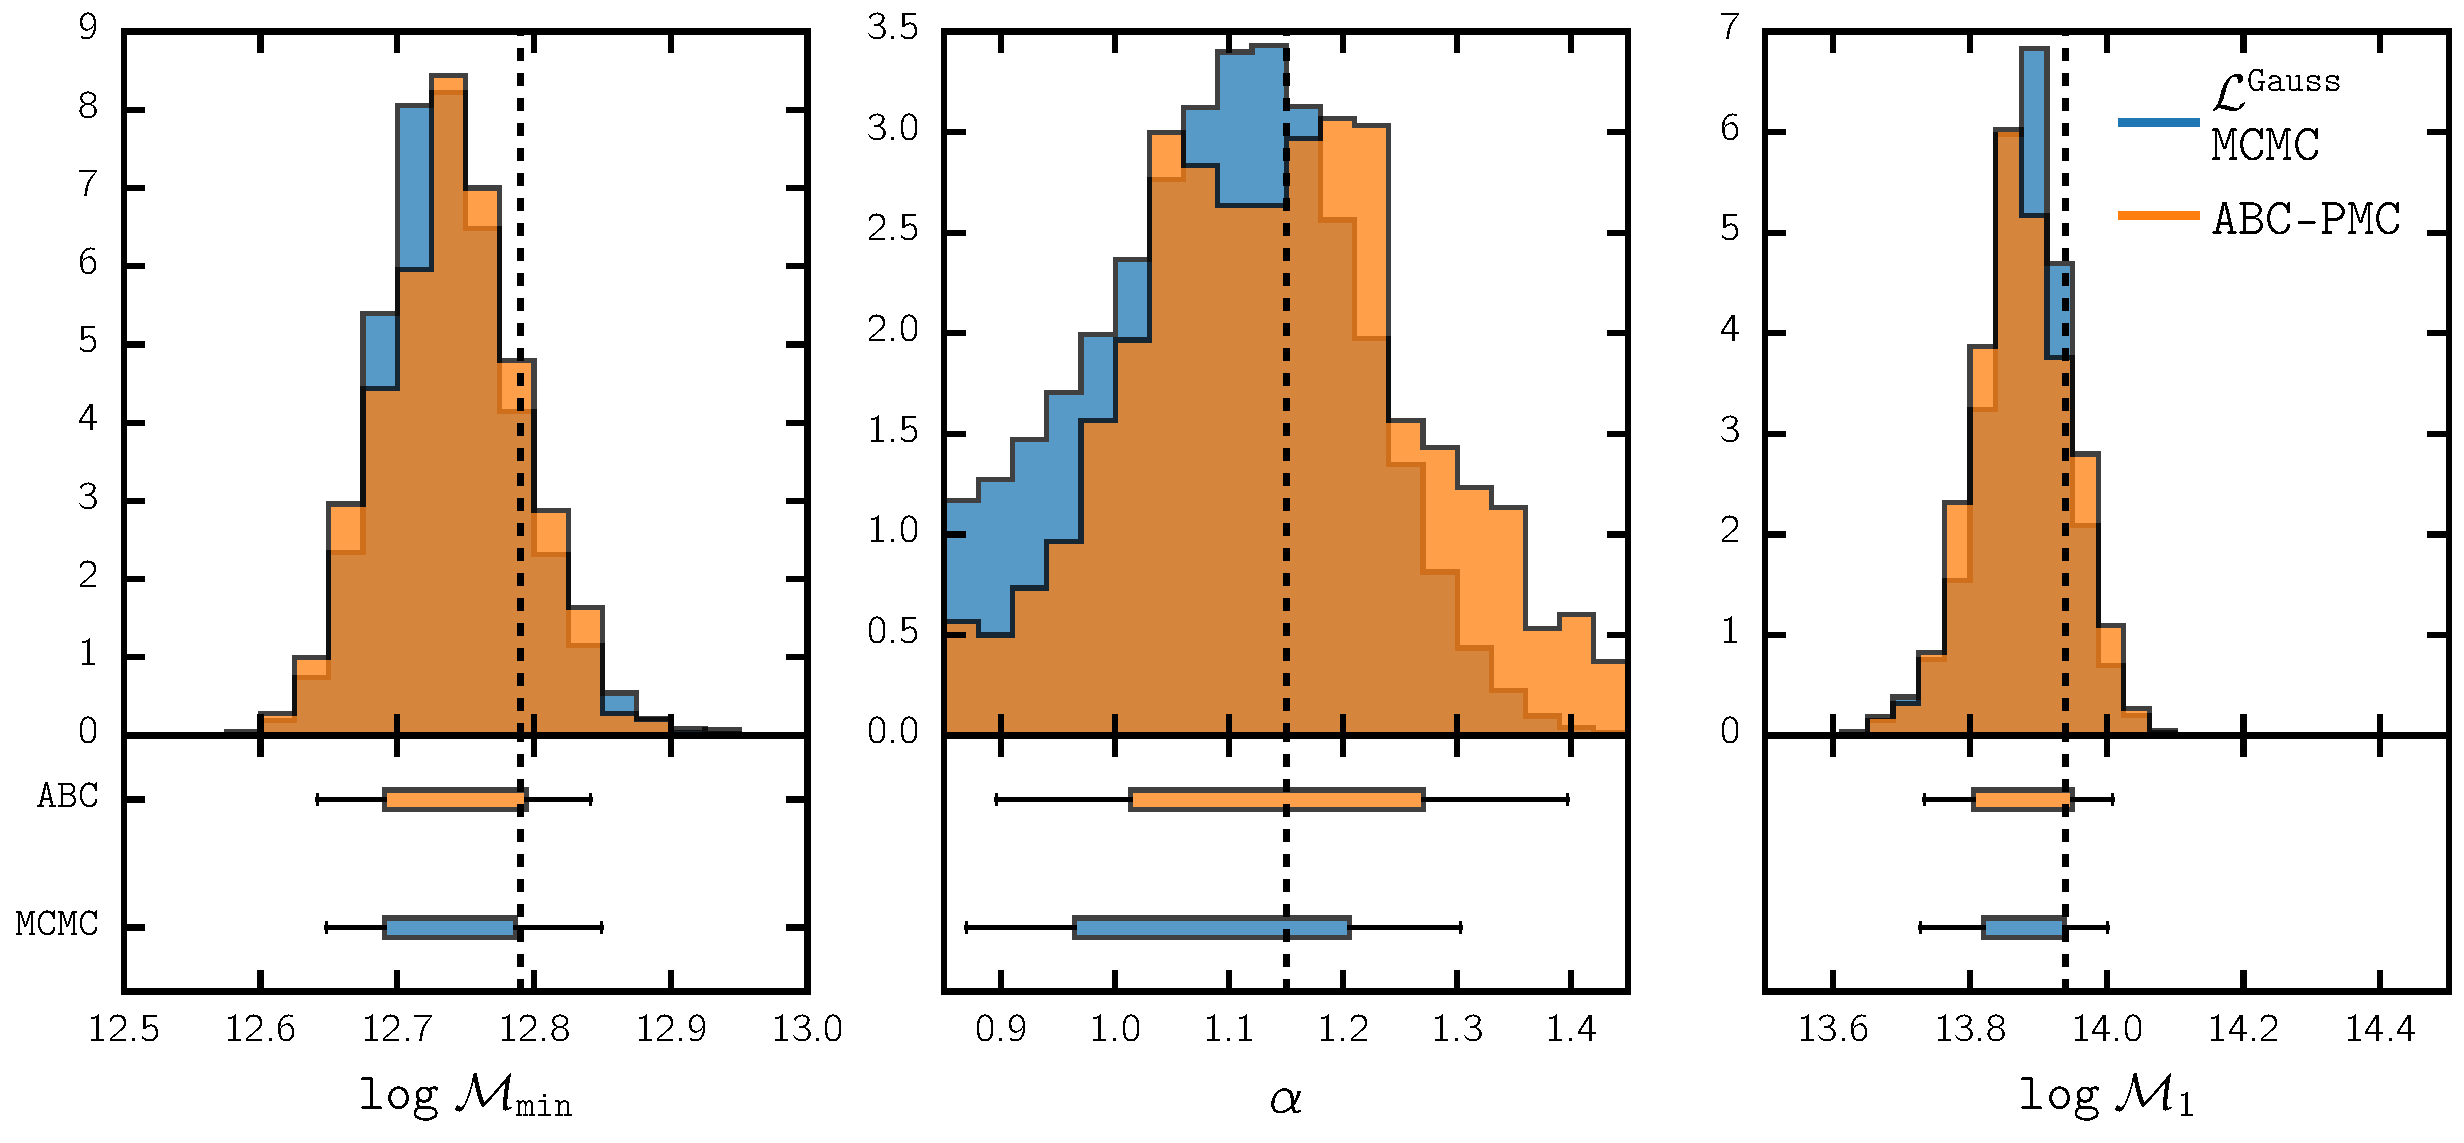
\includegraphics[width=1.\textwidth]{figures/abc/paper_ABCvsMCMC_nbargmf.pdf}
\caption{\label{fig:hist_nbargmf} 
Same as Figure \ref{fig:hist_nbarxi}, but both the ABC-PMC
analysis and the Gaussian pseudo-likelihood MCMC analysis use $\ngalaxy$ and $\gmf(N)$ as 
observables. Both methods derive constraints consistent with the ``true'' HOD parameters 
and infer the region of allowed values to similar precision. We note that the MCMC constraint 
on $\alpha$ is slightly more biased compared to ABC-PMC estimate. This discrepancy may stem 
from the fact that the use of Gaussian pseudo-likelihood and its associated assumptions is more 
spurious when modeling the group multiplicity function.}
%\end{center}
\end{figure*}

%%%%%%%%%%%%%%%%%%%%%%%%%%%%%%%%%%%%%%%%%%%%%%%%%%%%%%%%
% ABC vs MCMC Contours nbar +xi
%%%%%%%%%%%%%%%%%%%%%%%%%%%%%%%%%%%%%%%%%%%%%%%%%%%%%%%%
\begin{figure*}
%\begin{center}
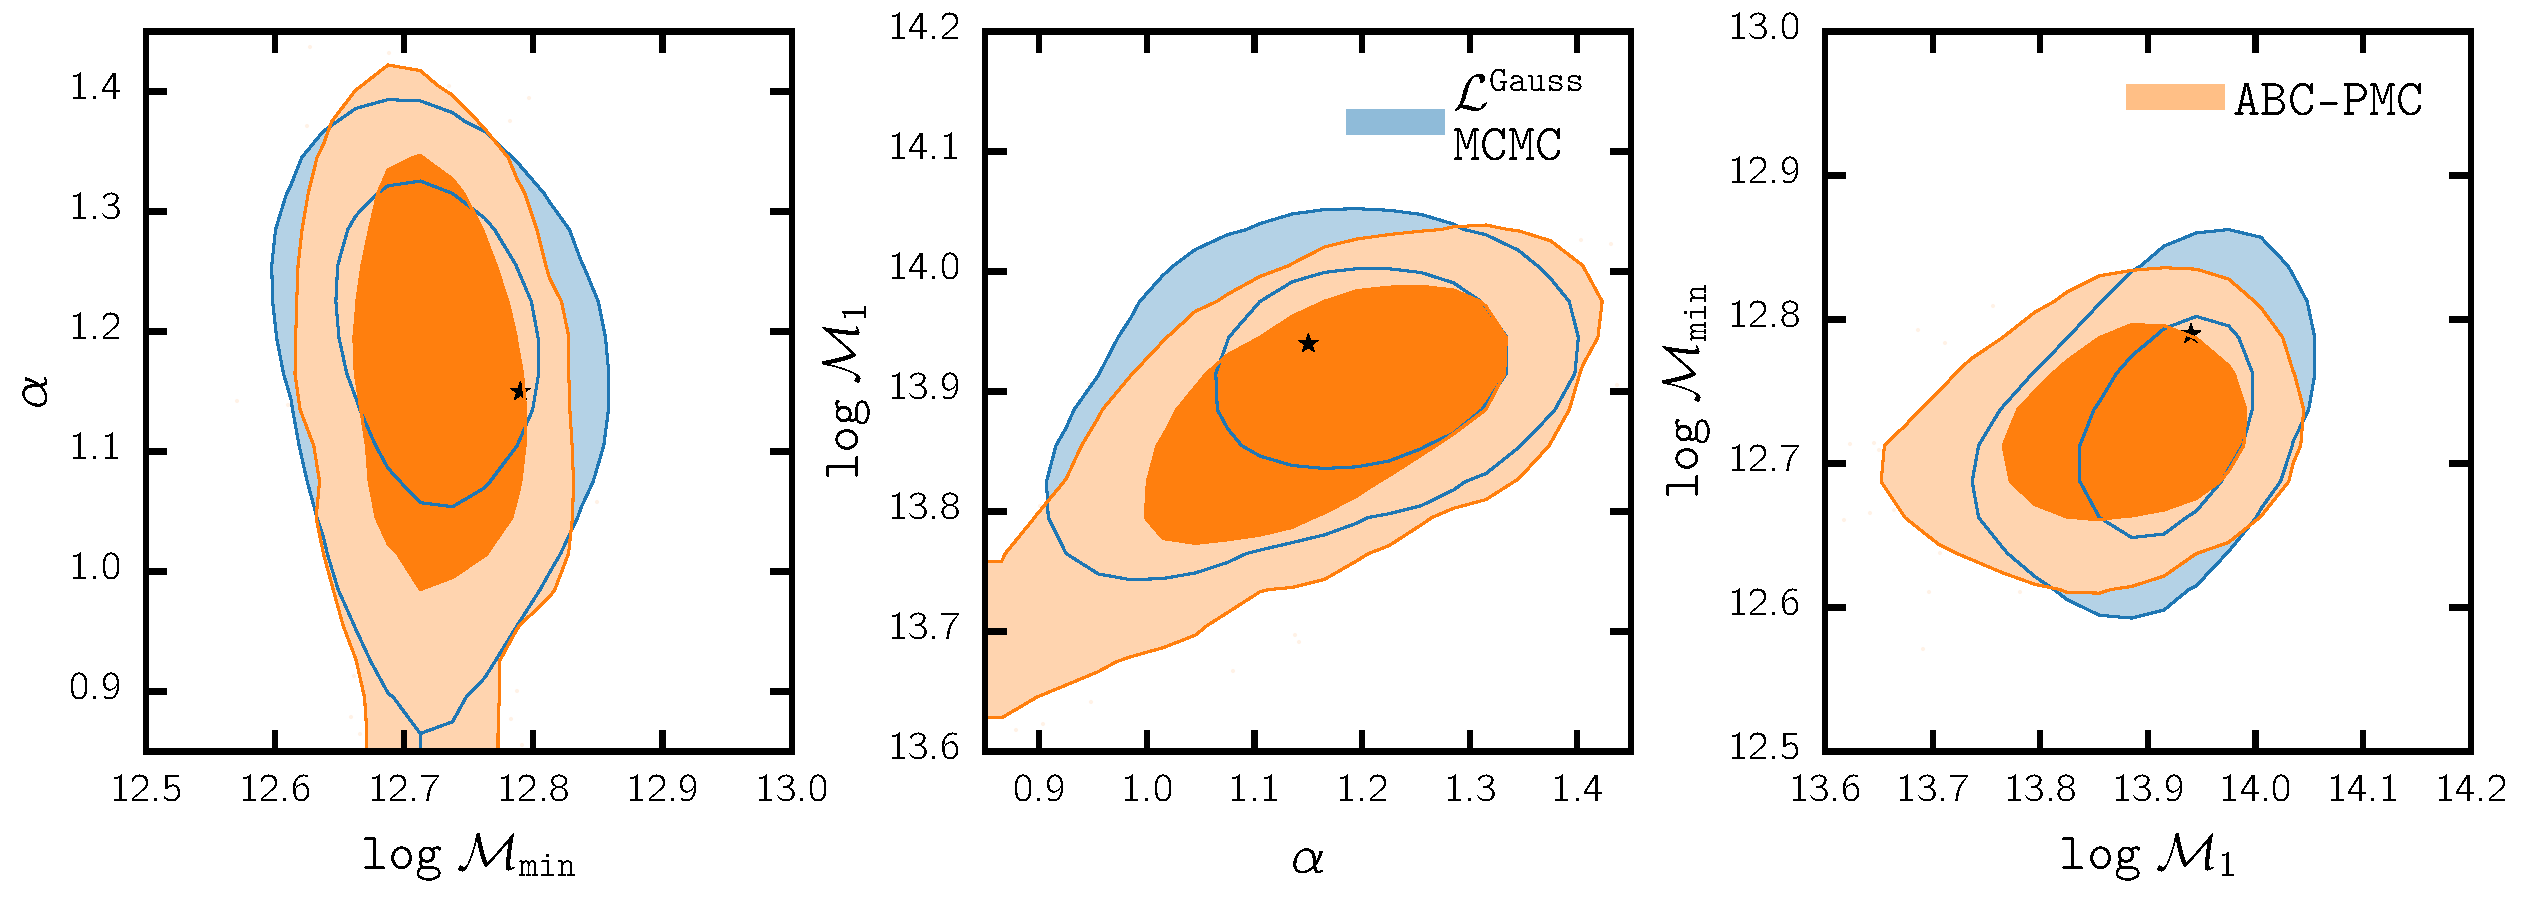
\includegraphics[width=1.\textwidth]{figures/abc/paper_ABCvsMCMC_contour_nbarxi.pdf}
\caption{\label{fig:cont_nbarxi}
We compare the ABC-PMC (orange) and the Gaussian pseudo-likelihood MCMC (blue)
predictions of the 68\% and 95\% posterior confidence regions over the HOD 
parameters ($\log \mathcal{M}_{\rm min}$, $\alpha$, and $\log \mathcal{M}_{1}$) 
using $\ngalaxy$ and $\xigg(r)$ as observables. In each panel, the black star
represents the ``true'' HOD parameters used to generate the mock observations. 
Both inference methods derive confidence regions consistent with the ``true'' 
HOD parameters.}
%\end{center}
\end{figure*}

\begin{figure*}
%\begin{center}
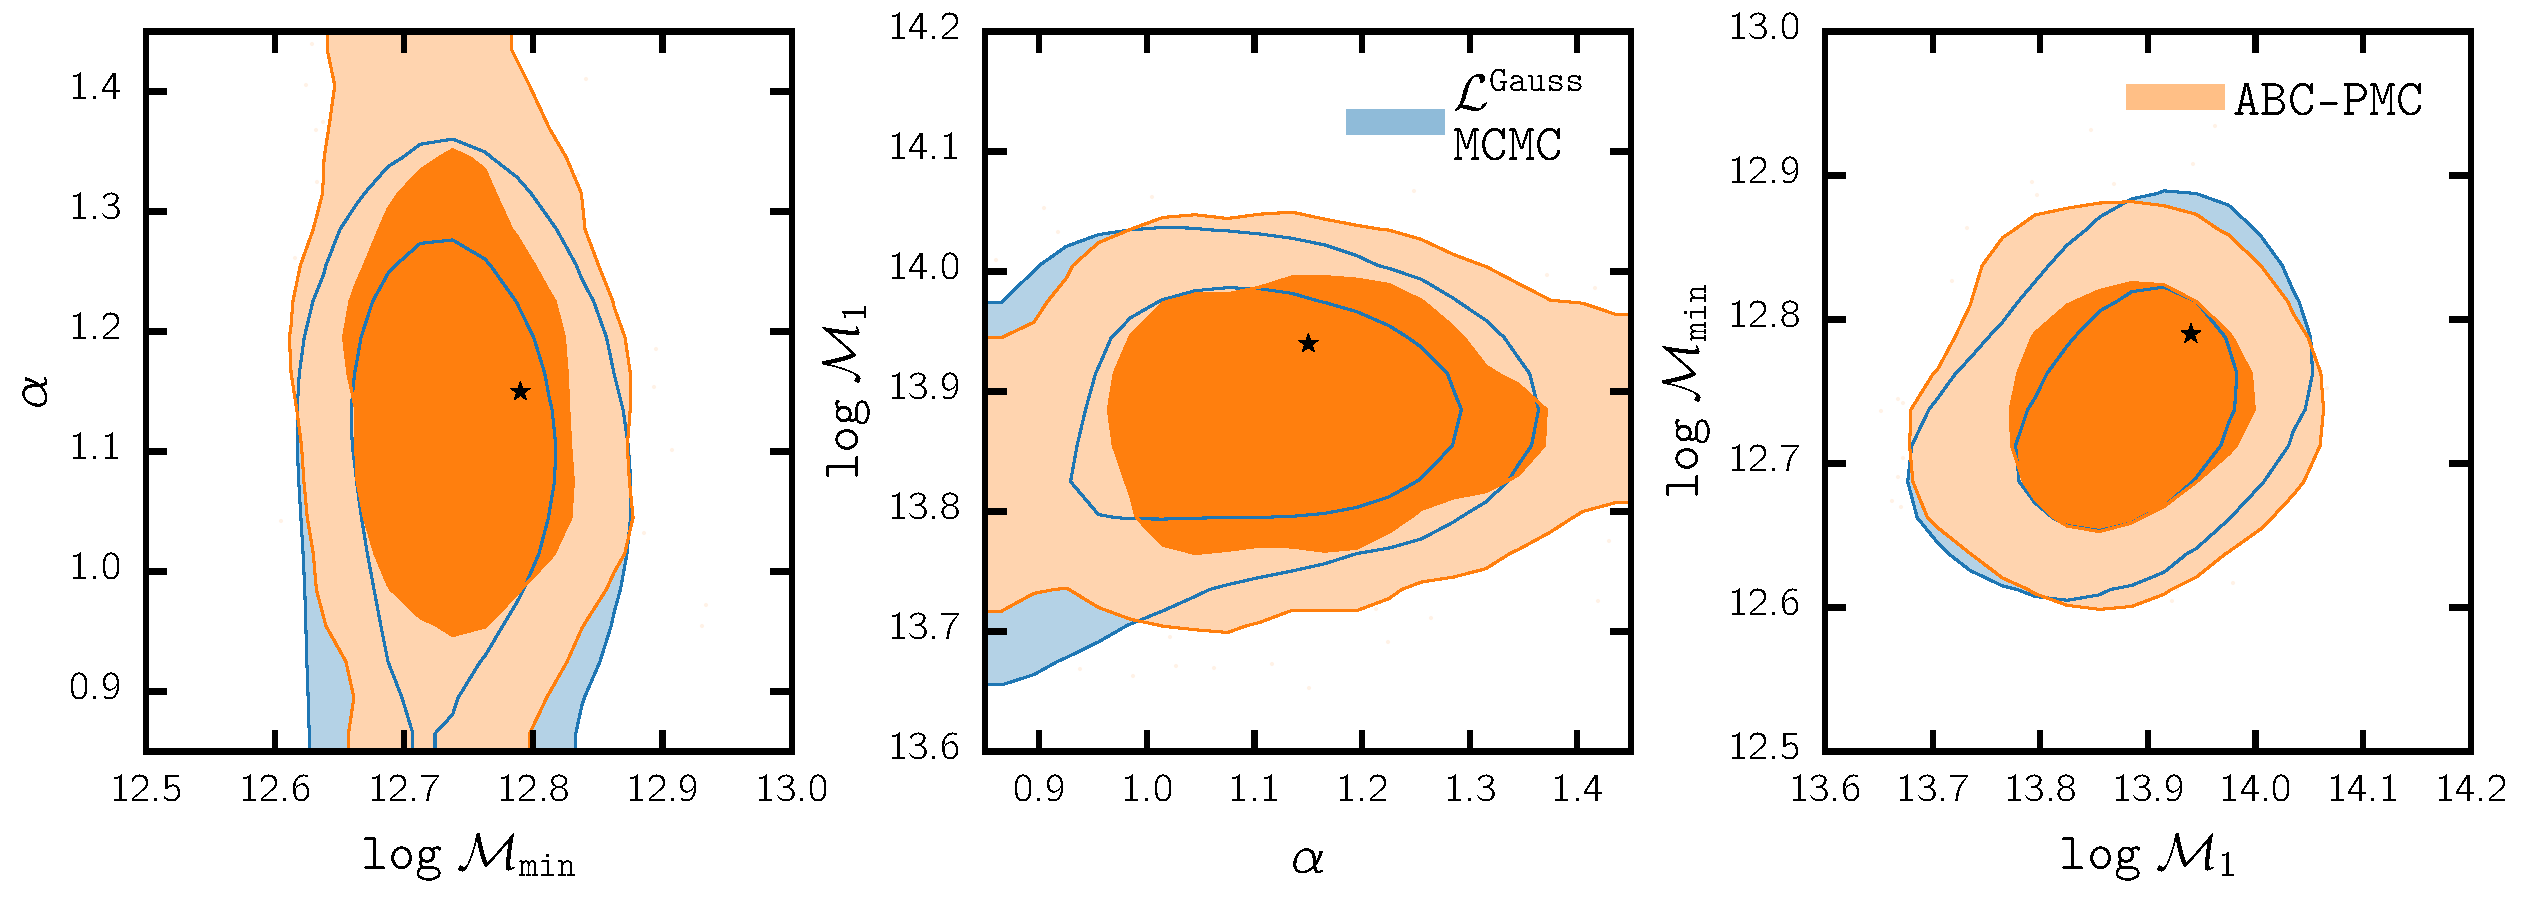
\includegraphics[width=1.\textwidth]{figures/abc/paper_ABCvsMCMC_contour_nbargmf.pdf}
\caption{\label{fig:cont_nbargmf} 
Same as Figure \ref{fig:cont_nbarxi}, but using $\ngalaxy$ and $\gmf(N)$ as 
observables. Again, the confidence regions derived from both methods are 
consistent with the ``true'' HOD parameters used to generate the mock 
observations. The confidence region of $\alpha$ from the Gaussian 
pseudo-likelood method is biased compared to the ABC-PMC contours. 
This may be due to the fact that the true likelihood function that 
describes $\gmf(N)$ deviates significantly from the assumed Gaussian 
functional form.}
%\end{center}
\end{figure*}

%%%%%%%%%%%%%%%%%%%%%%%%%%%%%%%%%%%%%%%%%%%%%%%

%%%%%%%%%%%%%%%%%%%% REFERENCES %%%%%%%%%%%%%%%%%%
%\clearpage
% The best way to enter references is to use BibTeX:
%%%%%%%%%%%%%%%%%%%%%%%%%%%

% Don't change these lines
%\bsp	% typesetting comment





\chapter{How are galaxies assigned to halos? searching for assembly bias in SDSS clustering measurements\chaplabel{gambly}}

This \paper\ is joint work with ChangHoon~Hahn (NYU) and it is submitted to the \emph{Astrophysical Journal}.


\section {chapter abstract}
Clustering of dark matter halos has been shown to depend on halo properties beyond mass such as halo concentration, a phenomenon referred to as halo assembly bias. 
%%% 
Standard halo occupation models (HOD) in large scale structure studies assume that halo mass alone is sufficient in characterizing the connection between galaxies and halos. 
%%% 
%%% CHH: @MJV, this sentence is far too long and indirect (RE RefReport Minor #7)

Modeling of galaxy clustering can face systematic effects if the number of galaxies are correlated with other halo properties. Using the Small MultiDark-Planck high resolution $N$-body simulation and the measurements of the projected two-point correlation function and the number density of Sloan Digital Sky Survey (SDSS) DR7 main galaxy sample, we investigate the extent to which the dependence of halo occupation on halo concentration can be constrained, and to what extent allowing for this dependence can improve our modeling of galaxy clustering.  

%%% 

%%% 
From our constraints on HOD with assembly bias, suggests that satellite population is not correlated with halo concentration at fixed halo mass. 
%%% 
%%% CHH: @MJV, this sentence is also long and a bit difficult to comprehend -- clarify. 
Furthermore, in terms of the occupation of centrals at fixed halo mass, our results favor lack of correlation with halo concentration in the most luminous samples ($M_{\rm r}<-21.5,-21$), modest levels of correlation for $M_{\rm r}<-20.5,-20, -19.5$ samples, lack of correlation for $M_{\rm r}<-19,-18.5$ samples, and anti-correlation for the faintest sample $M_{\rm r}<-18$.
%%%

We show that in comparison with abundance-matching mock catalogs, our findings suggest qualitatively similar but modest levels of the impact of halo assembly bias on galaxy clustering. 
The effect is only present in the central occupation and becomes less significant in brighter galaxy samples.
Furthermore, by performing model comparison based on information criteria, we find that in most cases, the standard mass-only HOD model is still favored by the observations.

\section{Introduction}
Most theories of cosmology and large-scale structure formation under consideration today rely on the central assumption that galaxies reside in dark matter halos. 
%%%
Detailed study of the galaxy--halo connection is therefore critical in constraining cosmological models (by modeling galaxy clustering at non-linear scales) as well as providing a window into galaxy formation physics. 
%%%
One of the most powerful methods for describing the galaxy--halo connection is the halo occupation 
distribution (HOD, see \citealt{seljak2000, berlind_weinberg2002, scoccimarro2001, zheng2005, zheng07, leauthaud12, tinker2013, decorated, 2016arXiv160701782H}).

HOD is an empirical framework that provides an analytic prescription for the expected number of galaxies $N$ that reside in halos by specifying a probability distribution function $P(N|x)$ where $x$ is a property of the halo. 
%%%
The standard HOD model assumes that halo mass $M$ alone is sufficient in determining the galaxy population of a halo. 
%%%
%%% CHH: @MJV, what do you mean by "statistical properties of galaxies"? Their spacial statistics? 
In the standard model, the statistical properties of galaxies is governed by the halo mass.
%%%
Mathematically, this assumption can be written as $P(N|M,\{x\})=P(N|M)$ where $\{x\}$ is the set of all possible halo properties beyond halo mass $M$.

Despite this simplifying assumption, the models of galaxy--halo connection based on HOD have been successfully used in fitting the measurements of a wide range of statistics such as the projected two-point correlation function of galaxies, small scale redshift space distortion, three-point function, and galaxy--galaxy lensing with remarkable success (e.g. \citealt{zheng07,tinker_rsd2007,zehavi2011,leauthaud12,parejko2013,coupon2015,hod-3pcf,miyatake15,zu2015,hod_vs_sham}). 
HOD has been used in constraining the cosmological parameters through modeling the galaxy two-point correlation function (hereafter 2PCF) (\citealt{abazajian2005}), combination of 2PCF with mass-to-light ratio of galaxies (\citealt{tinker05}), redshift space distortions (\citealt{tinker_rsd2007}), mass-to-number ratio of galaxy clusters (\citealt{tinker2012}) galaxy-galaxy weak lensing (\citealt{vdb03,cacciato13,more13,vdb13}) in the main sample of galaxies
of the Sloan Digital Sky Survey (hereafter SDSS, \citealt{york2000}), and also the combination of galaxy clustering and galaxy-galaxy lensing (\citealt{more15}) in SDSS III Baryon Oscillation Spectroscopic Survey (BOSS, \citealt{boss}). Furthermore, HOD is implemented in producing mock galaxy catalogs in the BOSS survey (\citealt{pthalo,qpm}). It has also been used in galaxy evolution studies (\citealt{conroy2009,leauthaud12,behroozi13,hudson2015,zu2015,zu2016}).

The complexity of structure formation however, is not sufficiently modeled under the standard HOD framework. Numerous $N$-body simulations that examine the clustering of 
dark matter halos have demonstrated that halo clustering is correlated with the formation 
history of halos. That is, at a fixed halo mass, the halo bias is correlated 
with properties of halos beyond mass, such as the concentration, formation time, or etc. 
This phenomenon is known as halo assembly bias (see \citealt{sheth2004,gao2005, harker2006, weschler2006, gao2007,croton2007,wang2007,angulo2008,dalal2008,li2008,sunayama2016}). It has been claimed that there is support for halo assembly bias in observations of SDSS redMaPPer galaxy clusters (\citealt{miyatake2016}).

Furthermore, the halo occupation may also depend on the formation history of halos. Then we may expect the spatial statistics of galaxies to be tied to the halo properties beyond mass such as the concentration of halos. There have been many attempts in the literature at examining the dependence of halo occupation on environment of the halos. But the results are mixed, and there is very little consensus. \citet{tinker_void_2009} show that the properties of the galaxies that reside in voids can be explained by the halo mass in which they live, and their properties are independent of their large scale environment of the halos. \citet{tinker_density_hod} proposes an extension of the standard HOD model $P(N|M)$ such that the number of galaxies residing in a halo not only depends on the mass of the halo, but also on the large scale density contrast $P(N|M,\delta)$. Based on modeling the clustering and void statistics of the SDSS galaxies, \citet{edHOD-tinker} shows that the dependence of the expected number of central galaxies on large scale density is not very strong.    
By randomly shuffling the galaxies among host halos of similar mass in the Millenium simulation, \citet{croton2007} shows that assembly bias significantly impacts the galaxy two-point correlation functions. They also show that the effect is different for the faint and the bright samples.

%Based on a group catalog of SDSS galaxies, \citet{blanton_group_2007} find that shuffling of galaxy colors among groups of similar mass has very little effect (only a slight change in small scales: less than $\sim 300 \rm{kpc}$) on the clustering of galaxies. Based on an alternative group catalog, \citet{wang2013} shows that clustering of the central galaxies does not depend only on the halo mass, but also on additional parameters such as the specific star formation rate.
%\todo{I think this paragraph might be a bit misleading to the reader, I think the paper could do without it. %Your work doesn't incorporate galaxy properties, but only halo properties.}

Another family of empirical galaxy--halo connection models is \emph{Abundance} \emph{Matching}. In Abundance Matching models, galaxies are assumed to live in halos and are assigned luminosities or stellar masses by assuming a monotonic mapping. In this monotonic mapping, the abundance of the halos are matched to the abundance of some property of galaxies (\citealt{kravtsov2004,vale2004,tasitsiomi2004,conroy2009,guo2010,wetzel2010,Neisten2011,watson2012,rodriguez2012,kravstov2013,mao2015,chavez2016}). 
One of the most commonly used host halo properties in abundance matching is the maximum circular velocity of the host halo $V_\mathrm{max}$ that traces the depth of the gravitational potential well of the halo. Furthermore, a scatter is assumed in this mapping. Within this galaxy--halo connection framework, abundance matching models have been successfully used in modeling a wide range of the statistical properties of galaxies such as two-point correlation function (\citealt{reddick2013,lehman2015,hod_vs_sham}) as well as the group statistics of galaxies (\citealt{sham_gmf}). 

It has been shown that the abundance matching mock catalogs that use $V_{\rm max}$ (see \citealt{hw2013,arz2014}), or the ones that use some combination of $V_{\rm max}$ and host halo virial mass $M_{\rm vir}$ (see \citealt{lehman2015}) exhibit significant levels of assembly bias. 
That is, halo occupation in these models depends not only on halo mass, but also on other halo properties. This has been demonstrated by randomizing the galaxies among host halos in bins of halo mass, such that the HOD remains constant, and then comparing the difference in the 2PCF of the randomized catalog and that of the original mock catalog. 

Based on the projected 2PCF measurements of (\citealt{hw2013}) galaxy catalogs, \citet{arz2014} showed that after fitting the 2PCF measurements of these catalogs with the standard \emph{mass-only} HOD modeling, the inferred HOD does not match the \emph{true} halo occupation of these catalogs. That is, in the presence of assembly bias in a galaxy sample, one can fit the clustering of this sample with the standard \emph{mass-only} HOD, but that does not guarantee recovery of the true HOD parameters.


%In this work, we aim to investigate the dependence of halo occupation on halo concentration, and how this dependence can be constrained in the low-redshift universe with the measurements of the 2PCF of galaxies with a wide range of luminosities in the SDSS DR7 main galaxy sample. 
%%% CHH: Re-phrasing 
In this work, we aim to investigate the dependence of halo occupation on halo concentration and how this dependence can be constrained in the low-redshift universe by 2PCF measurements of galaxies in a wide range of luminosities in the SDSS DR7 main galaxy sample. 

%%%
In order to achieve this goal, we need to adopt a HOD model that takes into account 
a dependence on halo properties beyond mass. 
%%% CHH: Re-phrasing to address ref. report
A number of frameworks in the literature \citep{edHOD-tinker,edHOD-gillmartin,edHOD-weinberg} 
have proposed environment-dependent HOD models that take into account the large-scale density contrast. 
In this investigation, we use the following case of the decorated HOD framework \citep{decorated}.  
In our decorated HOD framework, at fixed halo mass, halos are populated with galaxies according to 
the standard HOD model. Then using a secondary halo property, halos are split into two populations
in halo mass bins: halos with the highest and lowest secondary property values. Afterwards, based
on the assembly bias amplitude parameter, the number of galaxies in the two populations are enhanced
or reduced. In this model, the assembly bias parameter is not be degenerate with the rest of the HOD 
parameters.
%%%

The advantage of this framework is that the more complex HOD model is identical to the underlying \emph{mass-only} HOD model in every respect, except that at a fixed halo mass, halos receive enhancement (decrements) in the number of galaxies they host according to the value of their secondary property. In order to constrain assembly bias along with the rest of the HOD parameters, we make use of the publicly available measurements of the projected 2PCF and number density measurements made by   
(\citealt{guo2015}). These measurements made use of the NYU Value-Added Galaxy Catalog (\citealt{Blanton2005}).

Furthermore, we discuss how taking assembly bias into account in a more complex HOD model can improve our modeling of galaxy clustering in certain brightness limits. Then, we make a qualitative comparison between the levels of the impact of assembly bias in our best-fit decorated HOD model on galaxy clustering, and the impact of assembly bias present in (\citealt{hw2013}) catalogs on galaxy clustering. Our comparison shows the levels of the impact of assembly bias on galaxy clustering seen in the predictions of both models follow the same trend. That is assembly bias is more prominent in lower luminosity-threshold samples and its impact on galaxy clustering is only significant on large scales (more than a few Mpc).

In order to investigate whether the additional complexity of the decorated HOD model is demanded by the galaxy clustering data, we perform a model comparison between the standard HOD model and the HOD model with assembly bias. We also discuss the effect of our choice of $N$-body simulation on our constraints, and previous works in the literature (\citealt{zentner2016}) based on smaller $N$-body simulations. In addition to analysis of the luminosity-threshold samples presented in \citet{zentner2016}, we consider the faintest ($M_{\rm r} < -18,-18.5$) and the brightest ($M_{\rm r}<-20.5$) galaxy samples. For the samples considered in both \citet{zentner2016} and this investigation, we compare the constraints on the expected levels of assembly bias. 



This \paper is structured as follows: In Section \ref{sec:gmethod} we discuss the $N$-body simulation, the two halo occupation modeling methods, and the details of the computation of model observables used in this investigation. Then in Section \ref{sec:gdata}, we discuss the data used in this study. 
In Section \ref{sec:ganalysis} we discuss the details of our inference analysis as well as the results. This includes description of the details of our inference setup. In Section \ref{sec:gresult} we discuss the constraints and their implications. This includes presentation of the constraints on the parameters of the two models, interpretation of the predictions of our constraints and their possible physical ramifications, assessment of the levels of assembly bias as predicted by our model constraints and its comparison with abundance matching mock catalogs, and finally model comparison. Finally, we discuss and conclude in Section \ref{sec:gsummary}.
Throughout this paper, unless stated otherwise, 
all radii and densities are stated in comoving units. 
Standard flat $\Lambda$CDM is assumed, and all cosmological 
parameters are set to the Planck 2015 best-fit estimates.

\section{Method}\label{sec:gmethod}

In this section, we discuss the ingredients of our modeling one-by-one. First, we discuss the simulation used in this study. Afterwards, we talk about the forward modeling of galaxy catalogs in the standard HOD modeling framework as well as the decorated HOD framework. Then, we provide an overview of the two summary statistics of the galaxy catalogs that we used in our inference.  

\subsection{Simulation}

For the simulations used in this work, we make use of the Rockstar (\citealt{rockstar}) halo catalogs in the $z=0$ snapshot of the Small MultiDark of Planck cosmology (referred to as $\mathtt{SMDP}$) (\citealt{multidark}). This high resolution $N$-body simulation (publicly available at \url{https://www.cosmosim.org}) was carried out using the 
%%% CHH: small typo
GADGET-2 (see \citealt{multidark} and references therein) code, 
%%%
following the Planck $\Lambda$CDM cosmological parameters 
$\Omega_{\rm m} = 0.307$, $\Omega_{\rm b} = 0.048$, $\Omega_{\Lambda} = 0.693$, $\sigma_{8} = 0.823$, $n_{\rm s}=0.96$, 
$h=0.678$. The Box size for this $N$-body simulation is 0.4 $h^{-1} \rm{Gpc}$, the number of simulation particles is 3840$^3$, the mass per simulation particle $m_{\rm p}$ is $9.6 \times 10^{7} \; h^{-1} M_{\odot}$, and the gravitational softening length $\epsilon$ is 1.5 $h^{-1} \rm{kpc}$.

In the $\mathtt{SMDP}$ simulation, as discussed in \citet{halodemographic}, the Rockstar algorithm can reliably resolve halos with $\geq 100$
%%% CHH: grammar error
particles, which corresponds to $M_{\rm vir} \geq 9.6 \times 10^{9} \; h^{-1}M_{\odot}$.
%%%
%The advantage of using the $\mathtt{SMDP}$ simulation is that it satisfies both the size and resolution 
%requirements of studying the galaxy--halo connection in a wide range of luminosity thresholds. 
%%%
%%% Re-worded 

The $\mathtt{SMDP}$ simulation provides a number of advantages by satisfying both the size 
and resolution requirements of studying the galaxy--halo connection in a wide range of 
luminosity thresholds. For fainter galaxy samples, the faintest galaxies reside in lower 
mass halos, which requires high resolution. Meanwhile for luminous galaxy samples, their 
lower number densities requires a large comoving volume. 

%%%
Furthermore, since we are studying the higher order halo occupation statistics, the concentration-dependence in particular, it is important to use a simulation that can resolve the internal structure of halos. 
%%% CHH: Re-worded based on (github issue #1)

In the context of Subhalo-Abundance Matching models, which requires subhalo completeness 
in the low mass limit, the $\mathtt{SMDP}$ simulation has been used to model the faintest 
galaxy samples in the SDSS data~\citep[see][]{hod_vs_sham}. 

%%%
The added advantage of using the $\mathtt{SMDP}$ simulation over some of the other industrial simulation boxes commonly used in the literature such as $\mathtt{Bolshoi}$ (\citealt{bolshoi,multidark}) simulation is its larger comoving volume. Larger volume makes this simulation more suitable for performing inference with $L_{\star}$ (corresponding to $M_{\rm r} \sim -20.44$, see \citealt{blanton2003}) and more luminous than $L_{\star}$ galaxy samples that occupy larger comoving volumes.

\subsection{Halo occupation modeling}
\subsubsection{standard model without assembly bias}\label{subsubsec:hod}

For our standard HOD model, we assume the HOD parameterization from \citet{zheng07}. 
According to this model, a dark matter halo can host a central galaxy and some number of satellite galaxies. The occupation of the central galaxies follows a nearest-integer distribution, 
and the occupation of the satellite galaxies follows a Poisson distribution. The expected number of centrals and satellites as a function of the host halo mass of $M_{h}$ are given by the following equations 
\begin{eqnarray}
\langle N_{\rm c}| M_{h} \rangle &=& \frac{1}{2}\Big[1+\Big(\frac{\log M_{h} - \log M_{\rm min}}{\sigma_{\log \rm{M}}} \Big) \Big], \label{hod:central}\\ 
\langle N_{\rm s} | M_{h} \rangle &=& \Big( \frac{M_{h} - M_{\rm{0}}}{M_{\rm 1}} \Big)^{\alpha}. \label{hod:satellite}
\end{eqnarray}

For populating the halos with galaxies, we follow the procedure described in \citet{2016arXiv160701782H}, and \citet{decorated}. The central galaxies are assumed to be at the center of the host dark matter halos. We assume that the central galaxies are at rest with respect to the bulk motion of the halos and their velocities are given by the velocity of the center of mass of their host halo. Note that this assumption is shown to be violated in brighter than $L_{\star}$ galaxy samples (see \citealt{guo2015}). But since we are not considering the redshift space 2PCF multipoles in our study, we do not expect this velocity bias to impact our inference. We place the satellite galaxies within the virial radius of the halo following a Navarro-Frenk-White profile (hereafter NFW; \citealt{nfw}). This approach is different from other simulation-based halo occupation modeling techniques (see \citealt{hod_vs_sham,zheng_guo}) in that the positions of the satellites are not assigned to the dark matter particles in the $N$-body simulation. 
%%% Missing citation
 
The concentration of the NFW profile is given by the empirical mass-concentration relation provided by \citet{nfw_c(M)}. 

%%%
The velocities of the satellite galaxies are given by two components. The first component is the velocity of the host halo. The second component is the velocity of the satellite galaxy with respect to the host halo which is computed following the solution to the NFW profile Jeans equations (\citealt{more2010}). We refer the readers to \citet{decorated} for a more comprehensive and detailed discussion of the forward modeling of the galaxy mock catalogs.

\subsubsection{Model with Assembly bias}\label{subsubsec:decorated}
Now let us provide a brief overview of HOD modeling with $\mathtt{Heaviside}$ $\mathtt{Assemblybias}$ (referred to as the decorated HOD) introduced in \citet{decorated}. At a fixed halo mass $M_{h}$, halos are split into two populations: population of halos with the 0.5-percentile of highest concentration, and population of halos with 0.5 percentile of lowest concentration. For simplicity, we call the first population ``type-1'' halos, and the second population ``type-2'' halos. In the decorated HOD model, the expected number of central and satellite galaxies at a fixed halo mass $M_{h}$ in the two populations are given by

\begin{eqnarray}
\langle N_{c,i} | M_{h},c\rangle &=& \langle N_{c} | M_{h}\rangle + \Delta N _{c,i}, \; i=1,2 \label{eq:decoratedcentral} \\
\langle N_{s,i} | M_{h},c\rangle &=& \langle N_{s} | M_{h}\rangle + \Delta N _{s,i}, \; i=1,2 \label{eq:decoratedsatellite}
\end{eqnarray}
where $\langle N_{c} | M_{h}\rangle$ and $\langle N_{s} | M_{h}\rangle$ are given by Eqs \ref{hod:central} and \ref{hod:satellite} respectively, and we have $\Delta N_{s,1} + \Delta N_{s,2} = 0$, and $\Delta N_{c,1} + \Delta N_{c,2} = 0$. These two conditions ensure the conservation of HOD. At a given host halo mass $M_{h}$, the central occupation of the the two populations follows a nearest-integer distribution with the first moment given by \ref{eq:decoratedcentral}; and the satellite occupation of the the two populations follows a Poisson distribution with the first moment given by \ref{eq:decoratedsatellite}.

In this occupation model, the allowable ranges that quantities $\Delta N_{c,1}$ and $\Delta N_{s,1}$ can take are given by 
\begin{eqnarray}
\mathrm{max} \{-\langle N_{c} | M_{h}\rangle, \langle N_{c} | M_{h}\rangle -1 \} \leq &\Delta N_{c,i}& \leq \mathrm{min} \{\langle N_{c} | M_{h}\rangle, 1-\langle N_{c} | M_{h}\rangle\}
 , \label{eq:cen-bounds} \\
-\langle N_{s} | M_{h}\rangle \leq & \Delta N_{s,i}& \leq \langle N_{s} | M_{h}\rangle. \label{eq:sat-bounds}
\end{eqnarray}
Afterwards, the assembly bias parameter $\mathcal{A}$ is defined in the following way:

\begin{eqnarray}
\Delta N_{\alpha , 1}(M_{h}) &=& |\mathcal{A_\alpha}| \Delta N_{\alpha , 1}^{\rm max}(M_{h}) \; \; \rm{if} \; \mathcal{A_\alpha} > 0,  \label{positive_A} \\
\Delta N_{\alpha , 1}(M_{h}) &=& |\mathcal{A_\alpha}| \Delta N_{\alpha , 1}^{\rm min}(M_{h}) \; \; \rm{if} \; \mathcal{A_\alpha} < 0, \label{negative_A}
\end{eqnarray}
where the subscript $\alpha = c , s$ stands for the centrals and satellites respectively, and $\Delta N_{\alpha , 1}^{\rm max}(M_{h})$, $\Delta N_{\alpha , 1}^{\rm min}(M_{h})$ are given by Eqs. \ref{eq:cen-bounds} and \ref{eq:sat-bounds}. 

For a given $\mathcal{A}_{\alpha}$, once $\Delta N_{\alpha,1}$ is computed using equation (\ref{positive_A})---if $\mathcal{A}_{\alpha}>0$---or equation (\ref{negative_A})---if $\mathcal{A}_{\alpha}<0$---, $\Delta N_{\alpha,2} = 1 - \Delta N_{\alpha,1}$ is computed. At a fixed halo mass $M_{h}$, once the first moments of occupation statistics for the $type$-1 and $type$-2 halos are determined, we perform the same procedure described in \ref{subsubsec:hod} to populate the halos with mock galaxies.

\subsubsection{Redshift-space distortion}

Once the halo catalogs are populated with galaxies, the real-space positions and velocities of all mock galaxies are obtained. The next step is applying a redshift-space distortion transformation by assuming plane-parallel approximation.
Our use of plane parallel approximation is justified because of the narrow redshift range of the SDSS main galaxy sample considered in this study.
If we assume that the $\hat{z}$ axis is the line-of-sight direction, then with the transformation $(X,Y,Z) \rightarrow (S_x,S_y,S_z) = (X , Y ,Z + v_{z}(1+z)/H(z))$
for each galaxy with the real space coordinates $(X,Y,Z)$, velocities $(v_x,v_y,v_z)$, and redshift $z$, we obtain the redshift-space coordinate of the produced mock galaxies. Here we assume $z \simeq 0$, and therefore transformation is given by $(X,Y,Z) \rightarrow (X,Y,Z+v_{z}/H_{0})$.   

\subsection{Model Observables}

As described in \citet{decorated} and \citet{2016arXiv160701782H}, this approach makes no appeal to the fitting functions used in the analytical calculation of the 2PCF. The accuracy of these fitting functions is limited (\citealt{tinker08,tinker10,watson13}). Our approach also does not face the known issues of the treatment of halo exclusion and scale-dependent bias that can lead to potential inaccuracies in halo occupation modeling (see \citealt{vdb13}). 

The projected 2PCF $w_{p}(r_{p})$ can be computed by integrating the 3D redshift space 2PCF $\xi(r_{p} , \pi)$ along the line-of-sight (where $r_{\rm p}$ and $\pi$ denote the projected and line-of-sight separation of galaxy pairs respectively):
\beq
w_{p}(r_{p}) = 2 \int_{0}^{\pi_{max}}\xi(r_{p} , \pi)\; d\pi
\label{los}
\eeq
For our 2PCF calculations, we use the $w_{\rm p}$ measurement functionality of the fast and publicly available pair-counter code $\mathtt{CorrFunc}$ (\citealt{corrfunc} , available at \url{https://github.com/manodeep/Corrfunc}). To be consistent with the SDSS measurements described in Section \ref{sec:gdata}, $w_{\rm{p}}(r_{\rm{p}})$ is obtained by the line-of-sight integration to $\pi_{max}=40 \; h^{-1}\rm{Mpc}$. Note that $w_{p}(r_{p})$ is measured in units of $h^{-1}\rm{Mpc}$. To be consistent with \citet{guo2015}, we use the same binning (as specified in Section \ref{sec:gdata}) to measure $w_{\rm p}$. In addition to the projected 2PCF, we use the number density given by the number of mock galaxies divided by the comoving volume of the $\mathtt{SMDP}$ simulation. 

Note that a full forward model of the data requires running the simulation at different redshifts, generation of light cones, accounting for the complex survey geometry and systematic errors such as fiber collisions. Using the $z=0$ output of the $\mathtt{SMDP}$ simulation in our forward model of the spatial distribution of galaxies is only an approximation. This approximation can be justified by the small redshift range of the SDSS DR7 main galaxy sample. As described in \citealt{zehavi2011}, using random catalogs with angular window function of the data in measurements of galaxy clustering accounts for the geometry of the data. As described in Section~\ref{sec:gdata}, the fiber collision correction method of \citealt{guo2012} is applied to the SDSS clustering measurements used in this study. Therefore we do not account for that effect in our forward model.

\section{Data}\label{sec:gdata}

We focus on the measurements made on the volume-limited luminosity-threshold main sample of galaxies in the SDSS spectroscopic survey. In this section, we briefly describe the measurements used in our study for finding constraints on the assembly bias as well as the HOD parameters.

The measurements consist of the number density $n_{g}$ and the projected 2PCF $w_{p}(r_{p})$ made by \citet{guo2015} for the volume-limited sample of galaxies in NYU Value Added Galaxy Catalog (\citealt{Blanton2005}) constructed from the SDSS DR7 main galaxy sample (\citealt{abazajian2009}). In particular, eight volume-limited luminosity-threshold samples are constructed with maximum absolute luminosity in $r$-band of -18, 18.5, -19, -19.5, -20, -20.5, -21, and -21.5. Qualitatively, these samples are constructed in a similar way to those constructed in \citet{zehavi2011}. For detailed differences between the samples in \citet{guo2015} and \citet{zehavi2011}, we refer the reader to the Table 1 and Table 2 in those papers respectively. 


The projected 2PCFs are measured in 12 logarithmic $r_{p}$ bins (in units of $h^{-1}\rm{Mpc}$) of width $\Delta \log(r_{\rm p}) = 0.2$, starting from $r_{\rm{p}} = 0.1 \; h^{-1}\rm{Mpc}$. For all luminosity threshold samples, the integration along the line-of-sight (\ref{los}) are performed to $\pi_{max}=40 \; h^{-1}\rm{Mpc}$. 

The 2PCF measurement of each luminosity-threshold sample is accompanied by a covariance matrix constructed using 400 jackknife sub-samples of the data. The number density measurements are also accompanied by uncertainties measured using the jackknife method. Furthermore, the covariance between the number denisty and the projected 2PCF measurements are neglected. As \citet{norberg} shows, parameter estimation using jackknife covariance matrices is conservative as the jackknife method overestimates the errors in the observations. 

The advantage of using these measurements is that the effects of fiber collision systematic errors on the two-point statistics are corrected for (with the method described in \citealt{guo2012}), and therefore, these measurements provide accurate small scale clustering measurements. The assembly bias parameters introduced in section \ref{sec:gmethod} can have a 10-percent level impacts on galaxy clustering (\citealt{decorated}). Presence of assembly bias in the satellite population impacts the very small-scale clustering (\citealt{decorated}). Moreover as \citet{sunayama2016} demonstrates, the scale-dependence of the halo assembly bias has a pronounced bump in the 1-halo to 2-halo transition regime (1$\sim$2 $h^{-1}\rm{Mpc}$). This scale can be impacted by fiber collision systematics. Precise investigation of the possible impact of this signal on the galaxy clustering modeling requires accurate measurements of 2PCF on small scales. 
The method of \citet{guo2012} is able to recover the true $\wpp$ with  $\sim 6\%$ accuracy in small scales ($r_{\rm{p}} = 0.1 \; h^{-1}\rm{Mpc}$) and with $\sim 2.5\%$ at relatively large scales $r_{\rm{p}} \sim 30 \; h^{-1}\rm{Mpc}$. 

Note that the comoving volume of the $N$-body simulation used in this investigation is 64 $\times 10^{6} \; h^{-3}\rm{Mpc}^{3}$ which is larger than the comoving volume of all the luminosity-threshold samples in the SDSS data considered in this study except the two most luminous samples. The comoving volumes of the $M_{\rm r}<-21, \; 21.5$ samples are 71.74 and 134.65 (in units of $10^{6} h^{-3}\rm{Mpc}^{3}$) respectively. Since we are not studying very large scale clustering ($r_{p,\; \rm max} \leq 25 \; h^{-1}\rm{Mpc}$), using a slightly smaller box for those samples is justified. 

\section{Analysis}\label{sec:ganalysis}

\subsection{Inference setup}\label{subsec:analysis}

Given the SDSS measurements described in Section \ref{sec:gdata}, we aim to constrain the HOD model without assembly bias (described in \ref{subsubsec:hod}), and the HOD model with assembly bias (described in \ref{subsubsec:decorated}) for each luminosity-threshold sample, by sampling from the posterior probability distribution $p(\theta|d) \propto p(d|\theta) \pi(\theta)$ where $\theta$ denotes the parameter vector and $d$ denotes the data vector. In the standard HOD modeling $\theta$ is given by
\beq
\theta = \{ \mmin,\;\sigmam,\;\mzero,\; \alpha,\;\mone \},
\eeq
and in the HOD modeling with assembly bias we have 
\begin{eqnarray}
\theta = \{\mmin,\; \sigmam, \;\mzero, \;\alpha, \;\mone,\;\acen,\; \asat \},
\end{eqnarray}
Furthermore, data (denoted by $d$) is the combination of $[n_{g}, w_{p}(r_{p})]$. The negative log-likelihood (assuming negligible covariance between $n_{g}$ and $w_{p}(r_{p})$) is given by
\begin{eqnarray}
-2\ln p(d|\theta) &=& \frac{[n^{\rm data}_{g}-n^{\rm model}_{g}]^{2}}{\sigma_{n}^{2}} + \Delta \wpp^{\rm T}\widehat{C^{-1}}\Delta \wpp \; + \; \rm{const.},
\label{eq:lnlike_wp}
\end{eqnarray}
where $\Delta \wpp$ is a 12 dimensional vector, $\Delta \wpp(\rpp) = \wpp^{\rm data}(\rpp)-\wpp^{\rm model}(\rpp)$, and  $\widehat{C^{-1}}$ is the estimate of the inverse covariance matrix that is related to the inverse of the jackknife covariance matrix (provided by \citealt{guo2015}) $\widehat{C}^{-1}$, following \citet{hartlap2007}:
\beq
\widehat{C^{-1}} = \frac{N -d - 2}{N -1} \; \widehat{C}^{-1},
\eeq
where $N=400$ is the number of the jackknife samples, and $d=12$ is the length of the data vector $w_{\rm p}$. Another important ingredient of our analysis is specification of the prior probabilities $\pi(\theta)$ over the parameters of the halo occupation models considered in this study. For both models, we use uniform flat priors for all the parameters. The prior ranges are specified in the Table \ref{tab:prior2}. Note that a uniform prior between -1 and 1 is chosen for assembly bias parameters since these parameters are, by definition, bounded between -1 and 1. 
\begin{table}
\begin{center}
  \label{tab:prior2}
  \caption{{\bf Prior Specifications}: The prior probability distribution 
  and its range for each of the parameters. 
  All mass parameters are in unit of $h^{-1}M_\odot$. The parameters marked by $*$ are only used in the Heaviside Assembly bias modeling and by definition are bounded between -1 and 1.}
\begin{tabular}{@{}lllll}
\\ \hline 
    Parameter & & Prior & & Range \\ \hline
  $\alpha$ & & Uniform & & [0.85, 1.45] \\
  $\sigmam$ & & Uniform & &  [0.05, 1.5] \\
  $\mzero$   & & Uniform & &  [10.0, 14.5] \\
  $\mmin$ & &   Uniform & &  [10.0, 14.0] \\
  $\mone$ & & Uniform & & [11.5, 15.0] \\ 
  $\acen^{*}$ & & Uniform & & [-1.0, 1.0] \\
  $\asat^{*}$ & & Uniform & & [-1.0, 1.0] \\
 \hline
  \end{tabular}
\end{center}
\end{table}

For sampling from the posterior probability, given the likelihood function (see equation \ref{eq:lnlike_wp}) and the prior probability distributions (see Table \ref{tab:prior2}), we use the affine-invariant ensemble MCMC sampler (\citealt{goodmanweare}) and its implementation $\mathtt{emcee}$ (\citealt{emcee}). In particular, we run the $\mathtt{emcee}$ code with 20 walkers and we run the chains for at least 10000 iterations. We discard the first one-third part of the chains as burn-in samples and use the reminder of the chains as production MCMC chains. Furthermore, we perform Gelman-Rubin convergence test (\citealt{grtest}) to ensure that the MCMC chains have reached convergence.

\section{Results and Discussion}\label{sec:gresult}

\subsection{Constraints and Interpretations}
%Our constraints on the assembly bias parameters fall into two main categories. First, the satellite 
%assembly bias parameter $\asat$ and the second, the central assembly bias parameter $\acen$. 
%%% Re-worded
 In this section, we present the constraints derived for the two assembly 
bias parameters: the satellite assembly bias parameter ($\asat$) and the 
central assembly bias parameter $\acen$.  
%%%
As shown in Figure \ref{fig:bias}, for all the eight luminosity-threshold samples in the SDSS DR7 data, our constraints on the parameter $\asat$ are 
consistent with zero. On the other hand, our constraints on the parameter $\acen$--- albeit not tightly constrained--- show a trend which can be summarized as the following. In the most luminous galaxy samples, i.e. $M_{\rm r} < -21.5$ and $M_{\rm r} < -21$, $\acen$ is poorly constrained and the constraints are equivalent to zero. As we investigate less luminous samples, $M_{\rm r} < -20.5 , -20, -19.5$, our constraints on $\acen$ shift toward positive values, with the $M_{\rm r}<-20$ sample favoring the highest values for $\acen$. Furthermore, the posterior constraints on the assembly bias parameters in the slightly fainter samples, i.e. $M_{\rm r} < -19$ and i.e. $M_{\rm r} < -18.5$, are consistent with zero. In the faintest galaxy sample, i.e. $M_{\rm r} < -18$, our constraints favor negative values of $\acen$.

The underlying theoretical consideration for explaining the assembly bias of the central 
and satellite galaxies are different. The large scale clustering---or the two halo term in the galaxy clustering---is mainly governed by the clustering of the central galaxies. The central galaxy clustering can be thought as the weighted average over the halo clustering. The large scale bias of the dark matter halo clustering depends not only on mass, but also on the other properties of halos beyond mass, such as concentration (\citealt{weschler2006,gao2007,miyatake2016}), spin (\citealt{gao2007}), formation time (\citealt{gao2007, li2008}), and maximum circular velocity of the halo $V_{\rm max}$ (\citealt{sunayama2016}).

In particular, findings of \citet{weschler2006} and \citet{sunayama2016}
have demonstrated that for halos with mass bellow the collapse mass ($M \leq M_{\rm col} \simeq 10^{12.5}\; M_{\odot} $) the large scale bias of high-$V_{\rm max}$ (or equivalently high-$c$ halos at a fixed halo mass) is larger than that of the low-$V_{\rm max}$ (low-$c$ halos). This signal reverses and weakens for the high mass halos ($M \geq M_{\rm col}$). Note that the halo concentration traces the maximum circular velocity $V_{\rm max}$ such that halos with higher $V_{max}$ have higher concentration and vice versa (see \citealt{prada2012}). For halos described by NFW profile, at a fixed halo mass, halos with higher values of concentration have higher values of $V_{\rm max}$.

Furthermore, investigation of the scale dependence of halo assembly bias has shown that the ratio of the bias of high-$V_{\rm max}$ halos and the low-$V_{\rm max}$ halos has a bump-like feature in the quasi-linear scales $\sim$ 0.5 $\mathrm{Mpc}h^{-1}-5\mathrm{Mpc}h^{-1}$. From the theoretical standpoint, this phenomenon has been attributed to a population of distinct halos with $M \sim 10^{11.7} \; h^{-1}M_{\odot}$ at the present time that are close to the most massive groups and clusters (\citealt{sunayama2016}.

%, and see \citealt{more2016} for the observational investigation of this signal by means of galaxy-galaxy lensing). The clustering of these population of halos is therefore dictated by that of the massive halos. Note that this scale-dependent bias feature vanishes in high mass halos. %FIXME

Consequently, at a fixed halo mass less than $M_{\rm col}$, assignment of more central galaxies to the high-$c$ halos (higher expected number of central galaxies in the high-$c$ halos) gives rise to a boost in the galaxy clustering in the linear scales as well as in regimes corresponding to the one-halo to two-halo transition. For the more massive halos ($M \geq M_{\rm col}$), we expect the large-scale clustering boost to reverse sign, and the quasi-linear bump feature to vanish.  

Figure \ref{fig:wpmodel} demonstrates the 68$\%$ and 95$\%$ posterior predictions for the projected 2PCF $w_{p}$ from the occupation model without assembly bias (shown in red) and the occupation model with assembly bias (shown in blue) for all eight luminosity-threshold samples. For the brightest galaxies, $M_{r} < -21.5$ and $M_{r} < -21.0$, the posterior prediction of $w_{p}$ from the two models are consistent with one another. Note that these galaxies reside in the most massive halos ($M > M_{\rm col}$) for which the scale-dependence of the halo assembly bias and the difference between the large-scale bias of the high-$c$ and low-$c$ halos become negligible. 

Figure \ref{fig:wpres} shows the fractional difference between the 68$\%$ and 95$\%$ posterior predictions of $w_p$ and the SDSS data. It is evident from Figure \ref{fig:wpres} that some improvement on modeling the clustering of the samples of $L_{\star}$ and slightly less brighter than $L_{\star}$ galaxies can be achieved by employing the more complex halo occupation model with assembly bias. As a result of apportioning more central galaxies to the high-$c$ halos relative to the low-$c$ halos, in the samples with luminosity thresholds of $M_{\rm r}<-20.5, -20, -19.5$, the posterior predictions for $w_{p}$ are slightly improved in the intermediate scales ($1\sim 2 \; \mathrm{Mpc} h^{-1}$) and large scales. This can be also noted in significantly lower $\chi^{2}$ values---at the cost more model flexibility and higher degrees of freedom---achieved by the assembly bias model in these luminosity-threshold samples (see Table \ref{tab:constraints}).  

In the sample of galaxies with the luminosity threshold $M_{\rm r} < -19, -18.5$, the constraints on $\acen$ become consistent with zero with the tendency towards positive values for the $M_{\rm r}<-19$ sample and towards more negative values for the $M_{\rm r }<-18.5$ sample. As shown in Figures \ref{fig:wpmodel} and \ref{fig:wpres}, for the $M_{\rm r}<-19$ ($M_{\rm r}<-18.5$) sample this results in slightly higher (lower) posterior predictions for $w_{p}$ in the intermediate toward large scales. Overall, for these two samples, the assembly bias parameters remain largely unconstrained and the decorated HOD model does not yield better $\chi^{2}$ values. 

Finally, In the faintest sample ($M_{\rm r} < -18$), negative constraints on the parameter $\acen$ results in higher expected number of centrals in the low-$c$ halos, which at a fixed halo mass, cluster less strongly. This affects both the large scale bias and the intermediate regimes as a result of the scale-dependent bump feature (see Figures \ref{fig:wpmodel} and \ref{fig:wpres}). Furthermore, the model with assembly bias provides better fit to the SDSS data in this luminosity-threshold sample. 

The luminosity dependent trend in the constraints on the central assembly bias for the six dimmest samples can be attributed to the fact that the halo concentration is highly correlated with the maximum circular velocity $V_{\rm max}$ which is a tracer of the potential well of dark matter halos (\citealt{prada2012}). In a dark matter halo described by an NFW profile, the depth of the gravitational potential well of dark matter halos can be directly measured by the maximum circular velocity $V_{\rm max}$ (\citealt{vmax_potential}). In particular, the magnitude of the potential well at the center of an NFW halo---where the central galaxy is assumed to reside---scales as $V_{\rm max}^{2}$. More specifically, we have:
\beq
\Phi(r=0) = -\Big(\frac{V_{\rm max}}{0.465}\Big)^{2},
\eeq
 where $\Phi(r=0)$ is the central potential of an NFW profile. Note that $V_{\rm max}$ is also the quantity often used in the abundance matching technique in which the luminosity of galaxies is monotonically matched to $V_{\rm max}$ (see for example \citealt{reddick2013,lehman2015, hod_vs_sham, halodemographic}). The trend between the constraint on $\acen$ and the luminosity threshold of the samples may suggest that at a \emph{fixed} \emph{halo} \emph{mass}, the central galaxies in the dimmest samples ($M_{\rm r}<$-18 , -18.5) tend to reside in dark matter halos with shallower gravitational well. In brighter galaxy samples ($M_{\rm max}<$-19 , -19.5, -20, -20.5), at a \emph{fixed} \emph{halo} \emph{mass}, the central galaxies have a tendency to reside in dark matter halos with deeper gravitational potential well. 

The satellite assembly bias can only significantly alter the galaxy clustering at small-to-intermediate scales. Assigning more satellite galaxies to lower (or higher) concentration halos affects the one-halo term through increasing the satellite-satellite pair counts $\langle N_{\rm s} N_{\rm s} \rangle$. This results in boosting the small-scale clustering. But as pointed out by \citet{decorated}, the amount by which small-scale clustering increases also depends on the sign of the central assembly bias parameter $\acen$. Formation history of the halos can lead to the dependence of the abundance of subhalos on halo concentration (\citealt{zentner2005, mao2015}) at fixed halo mass, and since the occupation of the satellite galaxies is related to the abundance of subhalos, the satellite occupation may depend on halo concentration. 

However, our results suggest that for all the luminosity-threshold samples considered in this study, the satellite assembly bias parameter is largely unconstrained and consistent with zero. We do not expect the galaxy clustering data to be a sufficient statistics for obtaining constraints on the satellite assembly bias. Group statistics probes the high mass end of the galaxy--halo connection and is sensitive to the parameters governing the satellite population (see \citealt{sham_gmf, 2016arXiv160701782H}). Therefore these measurements may shed some light on potential presence of assembly bias in satellite population.   

It is important to note that the halo mass range in which the central assembly bias $\acen$ affects the central galaxy population is the mass range in which the condition $0<\langle N_{\rm c}|M \rangle<1$ is met. Consequently, larger scatter parameter $\sigmam$ increases the dynamical mass range in which assembly bias affects the galaxy clustering. Note that in the luminosity regimes for which we obtain tighter constraints on $\acen$, the best-estimate values of the scatter parameter $\sigmam$ appear to be higher in the model with assembly bias. This is evident in Figure \ref{fig:posterior}. The model with assembly bias tends to push $\sigmam$ to higher values. This can be attributed to the tendency of this model to increase the effective dynamical mass range of central assembly bias.

As shown in Table \ref{tab:constraints}, in the HOD model with assembly bias, the constraints found on the scatter parameter are not tight. This is in keeping with the results of \citet{guo2015} which uses the same SDSS measurements and finds that the scatter parameter remains largely unconstrained when only $n_{g}$ and $w_{p}$ are used as observables. Note that scatter is better constrained for the most luminous galaxy samples (this is attributed to the steep dependence of the halo bias and halo mass function on halo mass in the high mass end). But since these samples live in the most massive halos, we do not expect the tighter constraints on scatter to help us constrain the central assembly bias parameter. \citet{guo2015} shows that by employing additional measurements such as the monopole ($\xi_{0}$), quadruple ($\xi_{2}$), and hexadecapole ($\xi_{4}$), one can obtain tighter constraints on the scatter parameter. Tightening the constraints on the scatter parameter can lead to more precise inference of the central assembly bias parameter.    

As shown in Table \ref{tab:constraints}, our constraints on the underlying standard HOD model obtained from the model with assembly bias and the model without assembly bias are in good agreement. The only cases in which there are mild tensions between the constraints found from the two models on the underlying HOD parameters, are the $M_{\rm r}<-20$ and the $M_{\rm r}<-20.5$ samples. However, these tensions are still within one-sigma level. For instance, Figure \ref{fig:posterior} shows that in the $M_{\rm r}<-20.5$ sample, the constraint on the parameter $\alpha$ found from the model without assembly bias favor slightly higher values than the constraint found from the model with assembly bias. Also the scatter parameter $\sigmam$ is more tightly constrained in the standard HOD model. However, it is important to emphasize that these constraints are still in agreement with each other within a one-sigma level. 

\citet{arz2014} shows that in the mock catalogs that exhibit significant levels of assembly bias, using a simple mass-only occupation model can lead to considerable biases in inference of the galaxy--halo connection parameters. Although we cannot rule out moderate levels of assembly bias in our findings, we do not find any considerable discrepancy between the two models in terms of estimating the underlying HOD parameters. 
 
A few galaxy--halo connection methods have been proposed in the literature that give rise to assembly bias in the galaxy population. 
%%%% CHH: (Ref. Report Minor #5) re-worded and Conroy et al. (2006) included in citations. 
\citet{arz2014} demonstrates that the abundance matching techniques based on $V_{\rm max }$ \citep{conroy:2006aa,hw2013,reddick2013} exhibit some levels of assembly bias. 

We aim to provide a comparison between the impact of assembly bias on clustering in these mock catalogs and the mock catalogs predicted from our constraints on the decorated HOD model for $L_{\star}$-type galaxies. In particular, we consider the abundance matching catalogs produced by \citet{hw2013}. These catalogs have been extensively studied for examining potential systematic effects of galaxy assembly bias on cosmological (\citealt{edHOD-weinberg}) and halo occupation (\citealt{arz2014}) parameter inferences. 

This abundance matching catalog was built based on the $\mathtt{Bolshoi}$ $N$-body simulation (\citealt{bolshoi}) using the adaptive refinement tree code (ART \citealt{art}). The Box size for this simulation is 250 $h^{-1} \rm{Mpc}$, the number of simulation particles is 2048$^3$, the mass per simulation particle $m_{\rm p}$ is $1.35 \times 10^{8} \; h^{-1} M_{\odot}$, and the gravitational softening length $\epsilon$ is 1 $h^{-1} \rm{kpc}$. The halos and subhalos in this simulation are identified using the ROCKSTAR algorithm (\citealt{rockstar}). 
The \citealt{hw2013} catalogs make use of $V_{\rm peak}$ (maximum $V_{\rm max}$ throughout the assembly history of halo) as the subhalo property to be matched to galaxy luminosity. 

As noted by \citet{arz2014} and \citet{edHOD-weinberg}, these galaxy mock catalogs show significant levels of assembly bias in the central galaxy population. This has been demonstrated by investigating the difference in $w_{p}$ between the randomized mock catalogs and the original mock catalogs. Randomization is performed in a procedure described in \citet{arz2014} which we briefly summarize here: First, halos are divided into different bins of halo mass with width of 0.1 dex. Then all central galaxies are shuffled among all halos within each bin. Once the centrals have been shuffled, within each bin, the satellite systems are shuffled among all halos in that mass bin, preserving their relative distance to the center of halo. This procedure preserves the HOD, but erases any dependence of the galaxy population on the assembly history of halos. Therefore, assembly bias is erased in the randomized galaxy catalog. 

For $L_{\star}$ galaxies, the difference in $w_{p}$ between the randomized and the original catalogs of \citet{hw2013} is shown in Figure \ref{fig:randomized} with the red curves. As demonstrated in Figure \ref{fig:randomized} (and as previously noted by \citealt{arz2014,edHOD-weinberg}), the relative difference in $w_{p}$ is only significant in relatively large scales ($r_{p} > 1 \mathrm{Mpc} \; h^{-1}$). This implies that in these catalogs, only the central occupation is affected by assembly bias. This is in agreement with our findings. 

Furthermore, we investigate whether the impact of assembly bias on galaxy clustering predicted by our findings are in agreement with the abundance matching catalogs of \citet{hw2013}. First, we make random draws from the posterior probability distribution function over the parameters of the model with assembly bias. Then, we create mock catalogs with these random draws, and then we compute the difference in $w_{p}$ between the randomized catalogs and the original catalogs. The relative difference in $w_{p}$ predicted from our constraints are shown with blue curves in Figure \ref{fig:randomized}. 

We note that our findings follow the same trend. That is, we see negligible difference in the small scale clustering and more considerable differences in $w_{p}$ on larger scales ($r_{p} > 1\; \mathrm{Mpc}h^{-1}$). Similar to findings of \citet{arz2014}, \citet{lehman2015}, and \citet{edHOD-weinberg}, we see that the impact of assembly bias on galaxy clustering becomes less significant in brighter galaxy samples. Furthermore, we notice that our mock catalogs favor more moderate changes in galaxy clustering as a result of assembly bias. 

\begin{table*}
\begin{center}
  \label{tab:constraints}
 \caption{{\bf Constraints}: Constraints on the parameters of the HOD models with and without assembly bias. 
All mass parameters are in unit of $h^{-1}M_\odot$. The best-estimates and the error bars correspond to the 50$\%$ quantile and 68$\%$ confidence intervals obtained from the marginalized posterior probability pdfs. The last column is $\chi^{2}$ per degrees of freedom ($dof$), where $dof = N_{data} - N_{par}$}
\begin{tabular}{@{}lllllllllllllllllllllll}
\hline 
   $M_{\rm r,lim}$ & $\mmin$ & $\sigmam$ & $\mzero$ & $\alpha$ &  $\mone$ & $\acen$ & $\asat$ & $\chi^{2}/\rm{dof}$ \\  \hline
  \\ 
 -18 & $11.56^{+0.21}_{-0.25}$ &  $1.05^{+0.31}_{-0.52}$ & $10.84^{+0.77}_{-0.59}$ & $0.98^{+0.05}_{-0.05}$ &  $12.50^{+0.10}_{-0.10}$ & $-$ & $-$ & 14.51/8\\\\
     
  -18 & $11.53^{+0.23}_{-0.21}$ &  $1.08^{+0.28}_{-0.51}$ & $10.86^{+0.81}_{-0.62}$ & $0.97^{+0.05}_{-0.04}$ &  $12.56^{+0.09}_{-0.10}$ & $-0.67^{+0.55}_{-0.25}$ & $-0.30^{+1.09}_{-0.54}$ & 7.52/6\\ \\
     
-18.5 & $11.67^{+0.29}_{-0.25}$ &  $0.83^{+0.45}_{-0.53}$ & $10.85^{+0.64}_{-0.60}$ & $1.02^{+0.04}_{-0.04}$ &  $12.69^{+0.08}_{-0.08}$ & $-$ & $-$ & 6.17/8\\ \\
    
-18.5 & $11.60^{+0.31}_{-0.20}$ &  $0.74^{+0.49}_{-0.46}$ & $10.73^{+0.69}_{-0.51}$ & $1.01^{+0.05}_{-0.05}$ &  $12.72^{+0.09}_{-0.10}$ & $0.02^{+0.67}_{-0.62}$ & $0.07^{+0.53}_{-0.59}$ & 6.23/6\\ \\

-19 & $11.74^{+0.37}_{-0.18}$ &  $0.62^{+0.52}_{-0.39}$ & $10.82^{+0.62}_{-0.56}$ & $1.04^{+0.04}_{-0.04}$ &  $12.87^{+0.09}_{-0.09}$ & $-$ & $-$ & 8.69/8\\ \\

-19 & $11.71^{+0.37}_{-0.16}$ &  $0.58^{+0.53}_{-0.38}$ & $10.75^{+0.66}_{-0.52}$ & $1.03^{+0.04}_{-0.05}$ &  $12.90^{+0.10}_{-0.09}$ & $0.36^{+0.44}_{-0.62}$ & $-0.01^{+0.56}_{-0.54}$ & 8.87/6\\ \\

%%%%%%%wp%%%%%

-19.5 & $11.78^{+0.37}_{-0.13}$ &  $0.51^{+0.53}_{-0.31}$ & $11.09^{+0.69}_{-0.73}$ & $1.06^{+0.03}_{-0.04}$ &  $13.03^{+0.08}_{-0.07}$ & $-$ & $-$ & 6.80/8\\ \\

-19.5 & $11.82^{+0.41}_{-0.17}$ &  $0.62^{+0.54}_{-0.44}$ & $11.11^{+0.68}_{-0.77}$ & $1.03^{+0.04}_{-0.06}$ &  $13.03^{+0.10}_{-0.08}$ & $0.52^{+0.32}_{-0.47}$ & $-0.01^{+0.66}_{-0.49}$ & 5.56/6\\ \\

-20 & $12.01^{+0.17}_{-0.08}$ &  $0.32^{+0.32}_{-0.19}$ & $11.69^{+0.54}_{-0.99}$ & $1.08^{+0.03}_{-0.05}$ &  $13.32^{+0.08}_{-0.07}$ & $-$ & $-$ & 13.45/8\\ \\

-20 & $12.23^{+0.39}_{-0.24}$ &  $0.76^{+0.41}_{-0.43}$ & $11.66^{+0.62}_{-0.94}$ & $1.00^{+0.08}_{-0.05}$ &  $13.26^{+0.08}_{-0.09}$ & $0.81^{+0.12}_{-0.26}$ & $-0.15^{+0.33}_{-0.31}$ & 8.12/6\\ \\

-20.5 & $12.31^{+0.06}_{-0.06}$ &  $0.21^{+0.14}_{-0.11}$ & $12.36^{+0.27}_{-0.77}$ & $1.11^{+0.08}_{-0.08}$ &  $13.56^{+0.09}_{-0.09}$ & $-$ & $-$ & 11.40/8\\ \\

-20.5 & $12.37^{+0.16}_{-0.09}$ &  $0.44^{+0.28}_{-0.26}$ & $12.38^{+0.27}_{-0.54}$ & $1.05^{+0.08}_{-0.07}$ &  $13.60^{+0.10}_{-0.08}$ & $0.81^{+0.15}_{-0.43}$ & $-0.11^{+0.26}_{-0.27}$ & 6.82/6\\ \\

-21 & $12.73^{+0.14}_{-0.07}$ &  $0.32^{+0.22}_{-0.17}$ & $12.62^{+0.48}_{-1.36}$ & $1.17^{+0.10}_{-0.16}$ &  $14.01^{+0.08}_{-0.10}$ & $-$ & $-$ & 7.34/8\\ \\

-21 & $12.81^{+0.28}_{-0.11}$ &  $0.47^{+0.41}_{-0.25}$ & $12.51^{+0.61}_{-1.17}$ & $1.08^{+0.17}_{-0.13}$ &  $14.02^{+0.08}_{-0.10}$ & $0.33^{+0.51}_{-0.64}$ & $-0.18^{+0.41}_{-0.35}$ & 7.21/6\\ \\

-21.5 & $13.44^{+0.11}_{-0.09}$ &  $0.60^{+0.09}_{-0.11}$ & $12.57^{+0.77}_{-1.27}$ & $1.33^{+0.07}_{-0.21}$ &  $14.53^{+0.05}_{-0.07}$ & $-$ & $-$ & 3.29/8\\ \\

-21.5 & $13.43^{+0.12}_{-0.06}$ &  $0.60^{+0.12}_{-0.08}$ & $12.59^{+0.64}_{-1.25}$ & $1.27^{+0.11}_{-0.19}$ &  $14.54^{+0.05}_{-0.05}$ & $-0.24^{+0.50}_{-0.40}$ & $-0.30^{+0.86}_{-0.49}$ & 3.37/6\\ \\
                 
 \hline
  \end{tabular}
\end{center}
\end{table*}



\subsection{model comparison}

We want to address this question that whether the constraints on the model with assembly bias and the model without assembly bias given the galaxy clustering data lead us to claim that assembly bias is strongly supported by the observations or not. Within the standard HOD framework, the distribution of the galaxies is modeled using a simple description based on the $mass$-only ansatz: $P(N|M)$. The decorated HOD model however, provides a more complex description of the data by adding a secondary halo property (halo concentration in this study) and a more flexible occupation model: $P(N|M,c)$. 

In order to investigate whether the higher level of model complexity is demanded by the observations or not, we present model comparison between the models with and without assembly bias. In particular, we make use of two simple methods for model comparison: \emph{Akaike Information Criterion} (AIC, \citealt{aic} , see \citealt{gelmanic} for detailed discussion on AIC), and \emph{Bayesian Information Criteria} (BIC, \citealt{bic}). BIC and AIC are more computationally tractable than alternatives approaches such as computing the fully marginalized likelihood. The underlying assumption of these information criteria is that models that yield higher likelihoods are more preferable, but at the same time, models with more flexibility are penalized.

Suppose that $\mathcal{L}^{\star}$ is the maximum likelihood achieved by the model, $N_{\rm par}$ is the number of free parameters in the model, and $N_{\rm data}$ is the number of data points in the data set. Then we have

\begin{eqnarray}
\rm{BIC}&=& -2\;\ln \mathcal{L}^{\star} + N_{\rm par}\;\ln N_{\rm data} \; , \label{eq:bic} \\
\rm{AIC}&=& -2\;\ln \mathcal{L}^{\star} + 2N_{\rm par} \; . \label{eq:aic}
%         &+& 2\;\frac{N_{\rm par}(N_{\rm par}+1)}{N_{\rm data}-N_{\rm par}-1} \; . \label{eq:aic}
\end{eqnarray}

Given a data set, models with lower value of AIC and BIC are more desired. That is, in order for the higher model complexity (given by $N_{\rm par}$) to be justified, $\mathcal{L}^{\star}$ must be sufficiently higher. Therefore in this formulation, models that deliver lower information criteria scores are more preferable. 

Figure \ref{fig:ic} shows the comparison between the BIC and AIC scores for the model with assembly bias and the model without assembly bias. We note that the model without assembly bias is still preferable by the galaxy clustering observations. That is, although some improvements to fitting the clustering data can be achieved as a result of using a more complicated occupation model, these improvements are not significant enough to justify the use of a more complicated model that takes assembly bias into account. 

We note that both AIC and BIC scores improve in the luminosity-threshold samples for which, we have tighter constraints over the central assembly bias parameter. In particular, the model with assembly bias deliver \emph{only} \emph{slightly} lower AIC scores for the $M_{\rm r}<-18, -20$ samples. This supports our intuition that AIC and BIC penalize unconstrained parameters. Also note that, the difference between both BIC and AIC scores are marginal.

\subsection{choice of simulation}

Given the SDSS clustering measurements described in Section \ref{sec:gdata}, We repeat the inference of the assembly bias parameters $\asat$ and $\acen$ with the $\mathtt{BolshoiP}$ simulation (\citealt{multidark}). This $N$-body simulation is carried out with similar setting as the $\mathtt{Bolshoi}$ simulation with the exception that in the $\mathtt{BolshoiP}$ simulation, Planck cosmology is adapted and the mass per simulation particle is $1.49\times 10^8 \; h^{-1} M_{\odot}$. 

The summary of constraints are shown in Figure \ref{fig:bias_comparison}. In Figure \ref{fig:bias_comparison}, the constraints from the $\mathtt{SMDP}$ and the $\mathtt{BolshoiP}$ simulations are shown with circles and crosses respectively. Additionally, the upper and lower bounds on the inferred parameters reported by \citet{zentner2016} are shown in shaded blue regions. In the case of central assembly bias, all three constraints are consistent. For the luminosity-thresholds samples $M_{\rm r}<-20.5, -20, -19.5$, where the central assembly bias parameters are strongly positive, the constraints obtained from the $\mathtt{SMDP}$ simulation are tighter. 
  
In the case of the satellite assembly bias parameters however, constraints from the $\mathtt{BolshoiP}$ simulation for the luminosity threshold samples $M_{\rm r}<-20.5, -19$ favor more positive values of the parameter, while our constraints from the $\mathtt{SMDP}$ simulation for these two luminosity thresholds favor zero satellite assembly bias. As it is shown in the lower panel of Figure \ref{fig:bias_comparison}, our constraints from the $\mathtt{BolshoiP}$ simulations for the $M_{\rm r}<-21, -20.5, -20, -19.5, -19$ samples are consistent with the lower and upper bounds (shown with the shaded blue region) reported by \citet{zentner2016} that uses the same simulation but different $w_{p}$ measurements (\citealt{zehavi2011}). Therefore, there is some discrepancy between our $\asat$ constraints using the $\mathtt{SMDP}$ simulation and the $\mathtt{BolshoiP}$ simulations. 

For the $M_{\rm r}<-19, -20.5$ samples, the marginalized posterior PDFs over $\asat$ from the two simulations are shown in Figure \ref{fig:asat_comparison}. Note that $\asat$ is poorly constrained in both simulations and for both luminosity-threshold samples. For the $M_{\rm r}<-19$ sample, considering how poorly constrained the parameters are, the discrepancy between the constraints is not very stark. Note that the tension is still at a one-sigma level. The discrepancy however, becomes more pronounced in the $M_{\rm r}<-20.5$ sample. 

In terms of the effect of assembly bias on galaxy clustering, note that mocks created using the inferred parameters with the $\mathtt{SMDP}$ simulation show the same behavior as we observe in the abundance matching catalogs presented in \citet{arz2014} and \citet{lehman2015}. That is, the difference in $w_{p}$ between the mock catalogs and the randomized catalogs is mostly on large scales where the clustering is governed by the central galaxies. That is, the impact of assembly bias on the satellite occupation is negligible and only the central occupation is affected.  

\section{Summary and Conclusion}\label{sec:gsummary}

In this investigation, we provide constraints on the concentration-dependence of halo occupation for a wide range of galaxy luminosities in the SDSS data. In particular, the modeling is done in the context of the decorated HOD model \citet{decorated}, and the data used in this investigation is the projected 2PCF measurements published by \citet{guo2015}. We make use of $\mathtt{SMDP}$ high resolution $N$-body simulation that enables us to reliably perform inference for the faintest galaxy samples in the SDSS DR7 catalog that live in low mass halos, and the brightest galaxy samples that occupy large comoving volumes. 

Our findings suggest that the satellite assembly bias remains consistent with zero. However, our constraints on the central assembly bias parameter exhibit a trend with the luminosity limits of the galaxy samples. For the brightest samples, central assembly bias is consistent with zero, which is in agreement with this picture that the halo assembly bias becomes negligible for the most massive halos. 

For the $M_{\rm r}<-20.5, -20, -19.5$ samples, at a fixed halo mass, we find positive correlation between the central population and halo concentration at fixed halo mass. For $M_{\rm r}<-19, -18.5$ we find no correlation, and for the faintest sample, we find negative correlation. Given the large scale halo assembly bias and the scale-dependent feature of assembly bias in the quasi-linear scales, our constraints on the more flexible HOD model lead to improvement in modeling the galaxy clustering. However, we do not find these improvements to be sufficient to lower the information criteria scores associated with the more complex model. The exceptions are the $M_{\rm r}<-20,-18$ luminosity-threshold samples for which we find the strongest constraints on the central assembly bias. For these two samples, the HOD model with assembly bias yields lower BIC score than the model without assembly bias.

We compare the impact of assembly bias on galaxy clustering between the catalogs constructed from our results and the abundance matching catalogs presented in \citet{hw2013,arz2014}. We demonstrate that the effect of assembly bias on galaxy clustering predicted from our results is similar to (but more moderate than) the effects seen in the abundance matching catalogs of \citet{hw2013}. That is, assembly bias mostly affects the large scales and the quasi-linear clustering and the small scale clustering remains unaltered. In addition, the effect of assembly bias on galaxy clustering vanishes in the brightest galaxy samples.

Moreover, we repeat our inference using the $\mathtt{BolshoiP}$ simulation. 
We find that our findings based on the $\mathtt{BolshoiP}$ simulation are consistent with constraints reported by \citet{zentner2016} (in the $M_{\rm r}<-21, -20.5, -20, -19.5, -19$ luminosity-threshold samples) that predicts positive satellite assembly bias (correlation between the expected number of satellites and $V_{\rm max}$ at fixed host halo mass) for the $M_{\rm r}<-19, -20.5$ samples. However, we note that the results based on the $\mathtt{SMDP}$ simulation are more consistent with the picture provided by the previous models based on the abundance matching technique (e.g. \citealt{arz2014,lehman2015}). That is, only the large-scale clustering, governed by the centrals, is affected by assembly bias.

\section*{Acknowledgments}

We are grateful to David~W.~Hogg, Alex~I.~Malz, Andrew~Hearin, Andrew~Zentner, Chia-Hsun~Chuang, Michael~R.~Blanton, and Kilian~Walsh for discussions related to this work. This work was supported by the NSF grant AST-1517237. All the computations in this work were carried out in the New York University High Performance Computing Mercer facility. We thank Shenglong~Wang, the administrator of the NYU HPC center for his continuous and consistent support throughout the completion of this study. 

The CosmoSim database used in this paper is a service by the Leibniz-Institute for Astrophysics Potsdam (AIP). The MultiDark database was developed in cooperation with the Spanish MultiDark Consolider Project CSD2009-00064. The authors gratefully acknowledge the Gauss Centre for Supercomputing e.V. (www.gauss-centre.eu) and the Partnership for Advanced Supercomputing in Europe (PRACE, www.prace-ri.eu) for funding the MultiDark simulation project by providing computing time on the GCS Supercomputer SuperMUC at Leibniz Supercomputing Centre (LRZ, www.lrz.de).

All of the code written for this project is available in an open-source
code repository at \url{https://github.com/mjvakili/gambly}. The SDSS clustering measurements and the covariance matrices used in this work are available at \url{http://sdss4.shao.ac.cn/guoh/files/wpxi_measurements_Guo15.tar.gz}. Description of the $\mathtt{SMDP}$ and the $\mathtt{BolshoiP}$ halo catalogs used in this investigation can be found at \url{https://www.cosmosim.org/cms/simulations}. The RockStar halo catalogs of the $\mathtt{SMDP}$ and the $\mathtt{BolshoiP}$ simulations are publicly available at \url{http://yun.ucsc.edu/sims/SMDPL/hlists/index.html} and \url{http://yun.ucsc.edu/sims/Bolshoi_Planck/hlists/index.html} respectively. We thank Peter Behroozi for making the halo catalogs publicly available. In this work we have made use of the publicly available codes: corner (\citealt{corner}), emcee (\citealt{emcee}), halotools (\citealt{halotools}), Corrfunc (\citealt{corrfunc}), and changtools (\url{https://github.com/changhoonhahn/ChangTools}). The abundance matching mock catalogs used in this study are available at (\url{http://logrus.uchicago.edu/~aphearin/}).  



\clearpage

%%%%%%%%%%%%%%%% FIGURES %%%%%%%%%%%%%%

%%%%%%%%%%%%%%%%%%%%%%%%%%%%%%%%%%%%%%%%%%%%%%%%%%%%%%%%
% ACEN and ASAT constraints
%%%%%%%%%%%%%%%%%%%%%%%%%%%%%%%%%%%%%%%%%%%%%%%%%%%%%%%%
\begin{figure*}[p]~\\
\begin{center}
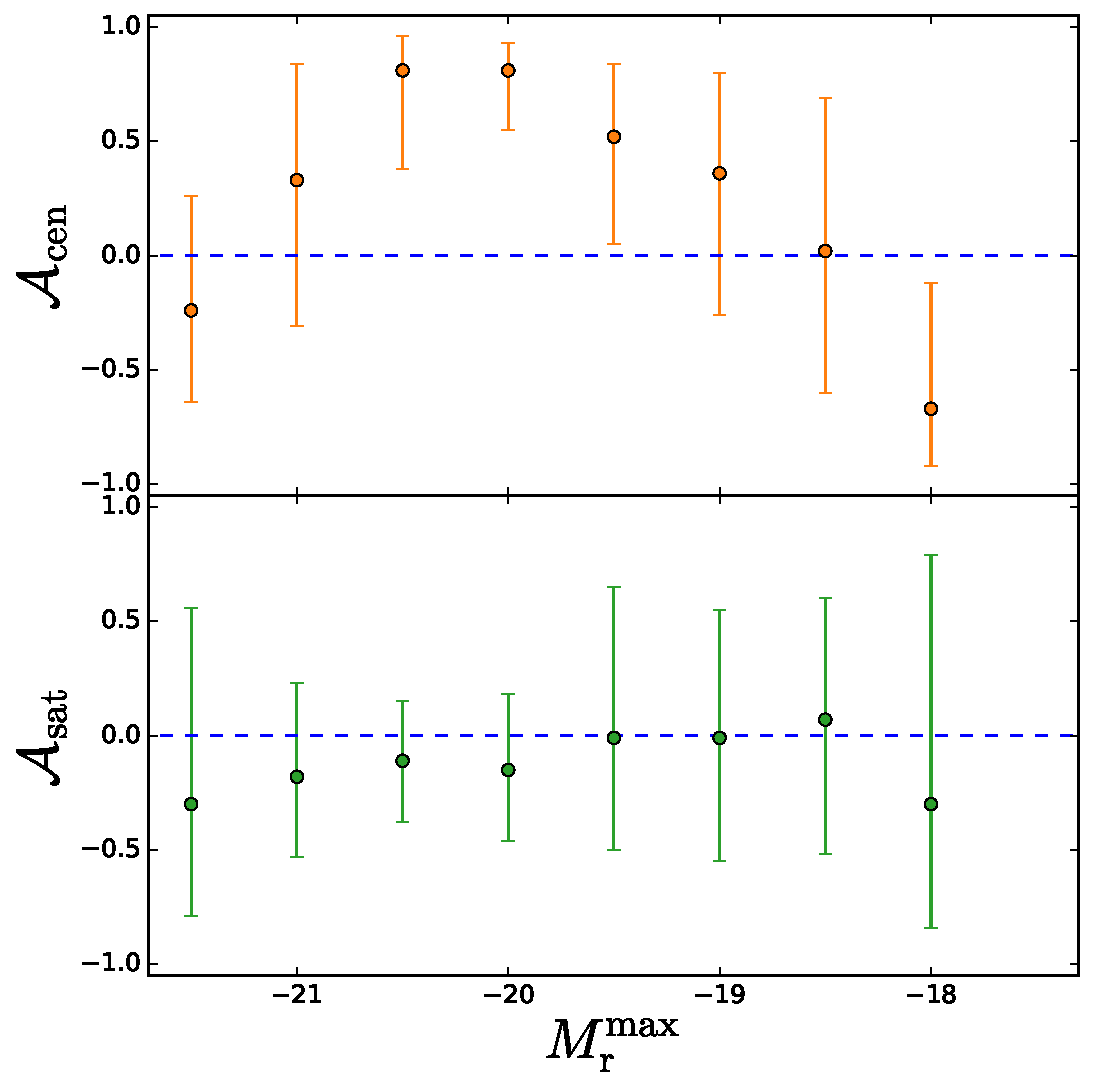
\includegraphics[width=0.8\textwidth]{figures/gambly/bias2.pdf}
\caption{Constraints on the central assembly bias $\acen$ (Top panel) and the satellite assembly bias $\asat$ (Bottom panel) parameters. The $\acen$ constraints for the $M_{\rm r} < -20.5, -20, -19.5$ samples favor positive values of $\acen$ with the tightest constraint coming from the $M_{\rm r} < -20$ sample. The $\acen$ constraints for the $M_{\rm r}<-18$ sample favor negative values of $\acen$. All the $\asat$ constraints are consistent with no satellite assembly bias.}
\label{fig:bias}
\end{center}
\end{figure*}

%\clearpage

%%%%%%%%%%%%%%%%%%%%%%%%%%%%%%%%%%%%%%%%%%%%%%%%%%%%%%%%
% WP MODEL
%%%%%%%%%%%%%%%%%%%%%%%%%%%%%%%%%%%%%%%%%%%%%%%%%%%%%%%%
\begin{figure*}[p]~\\
\begin{center}
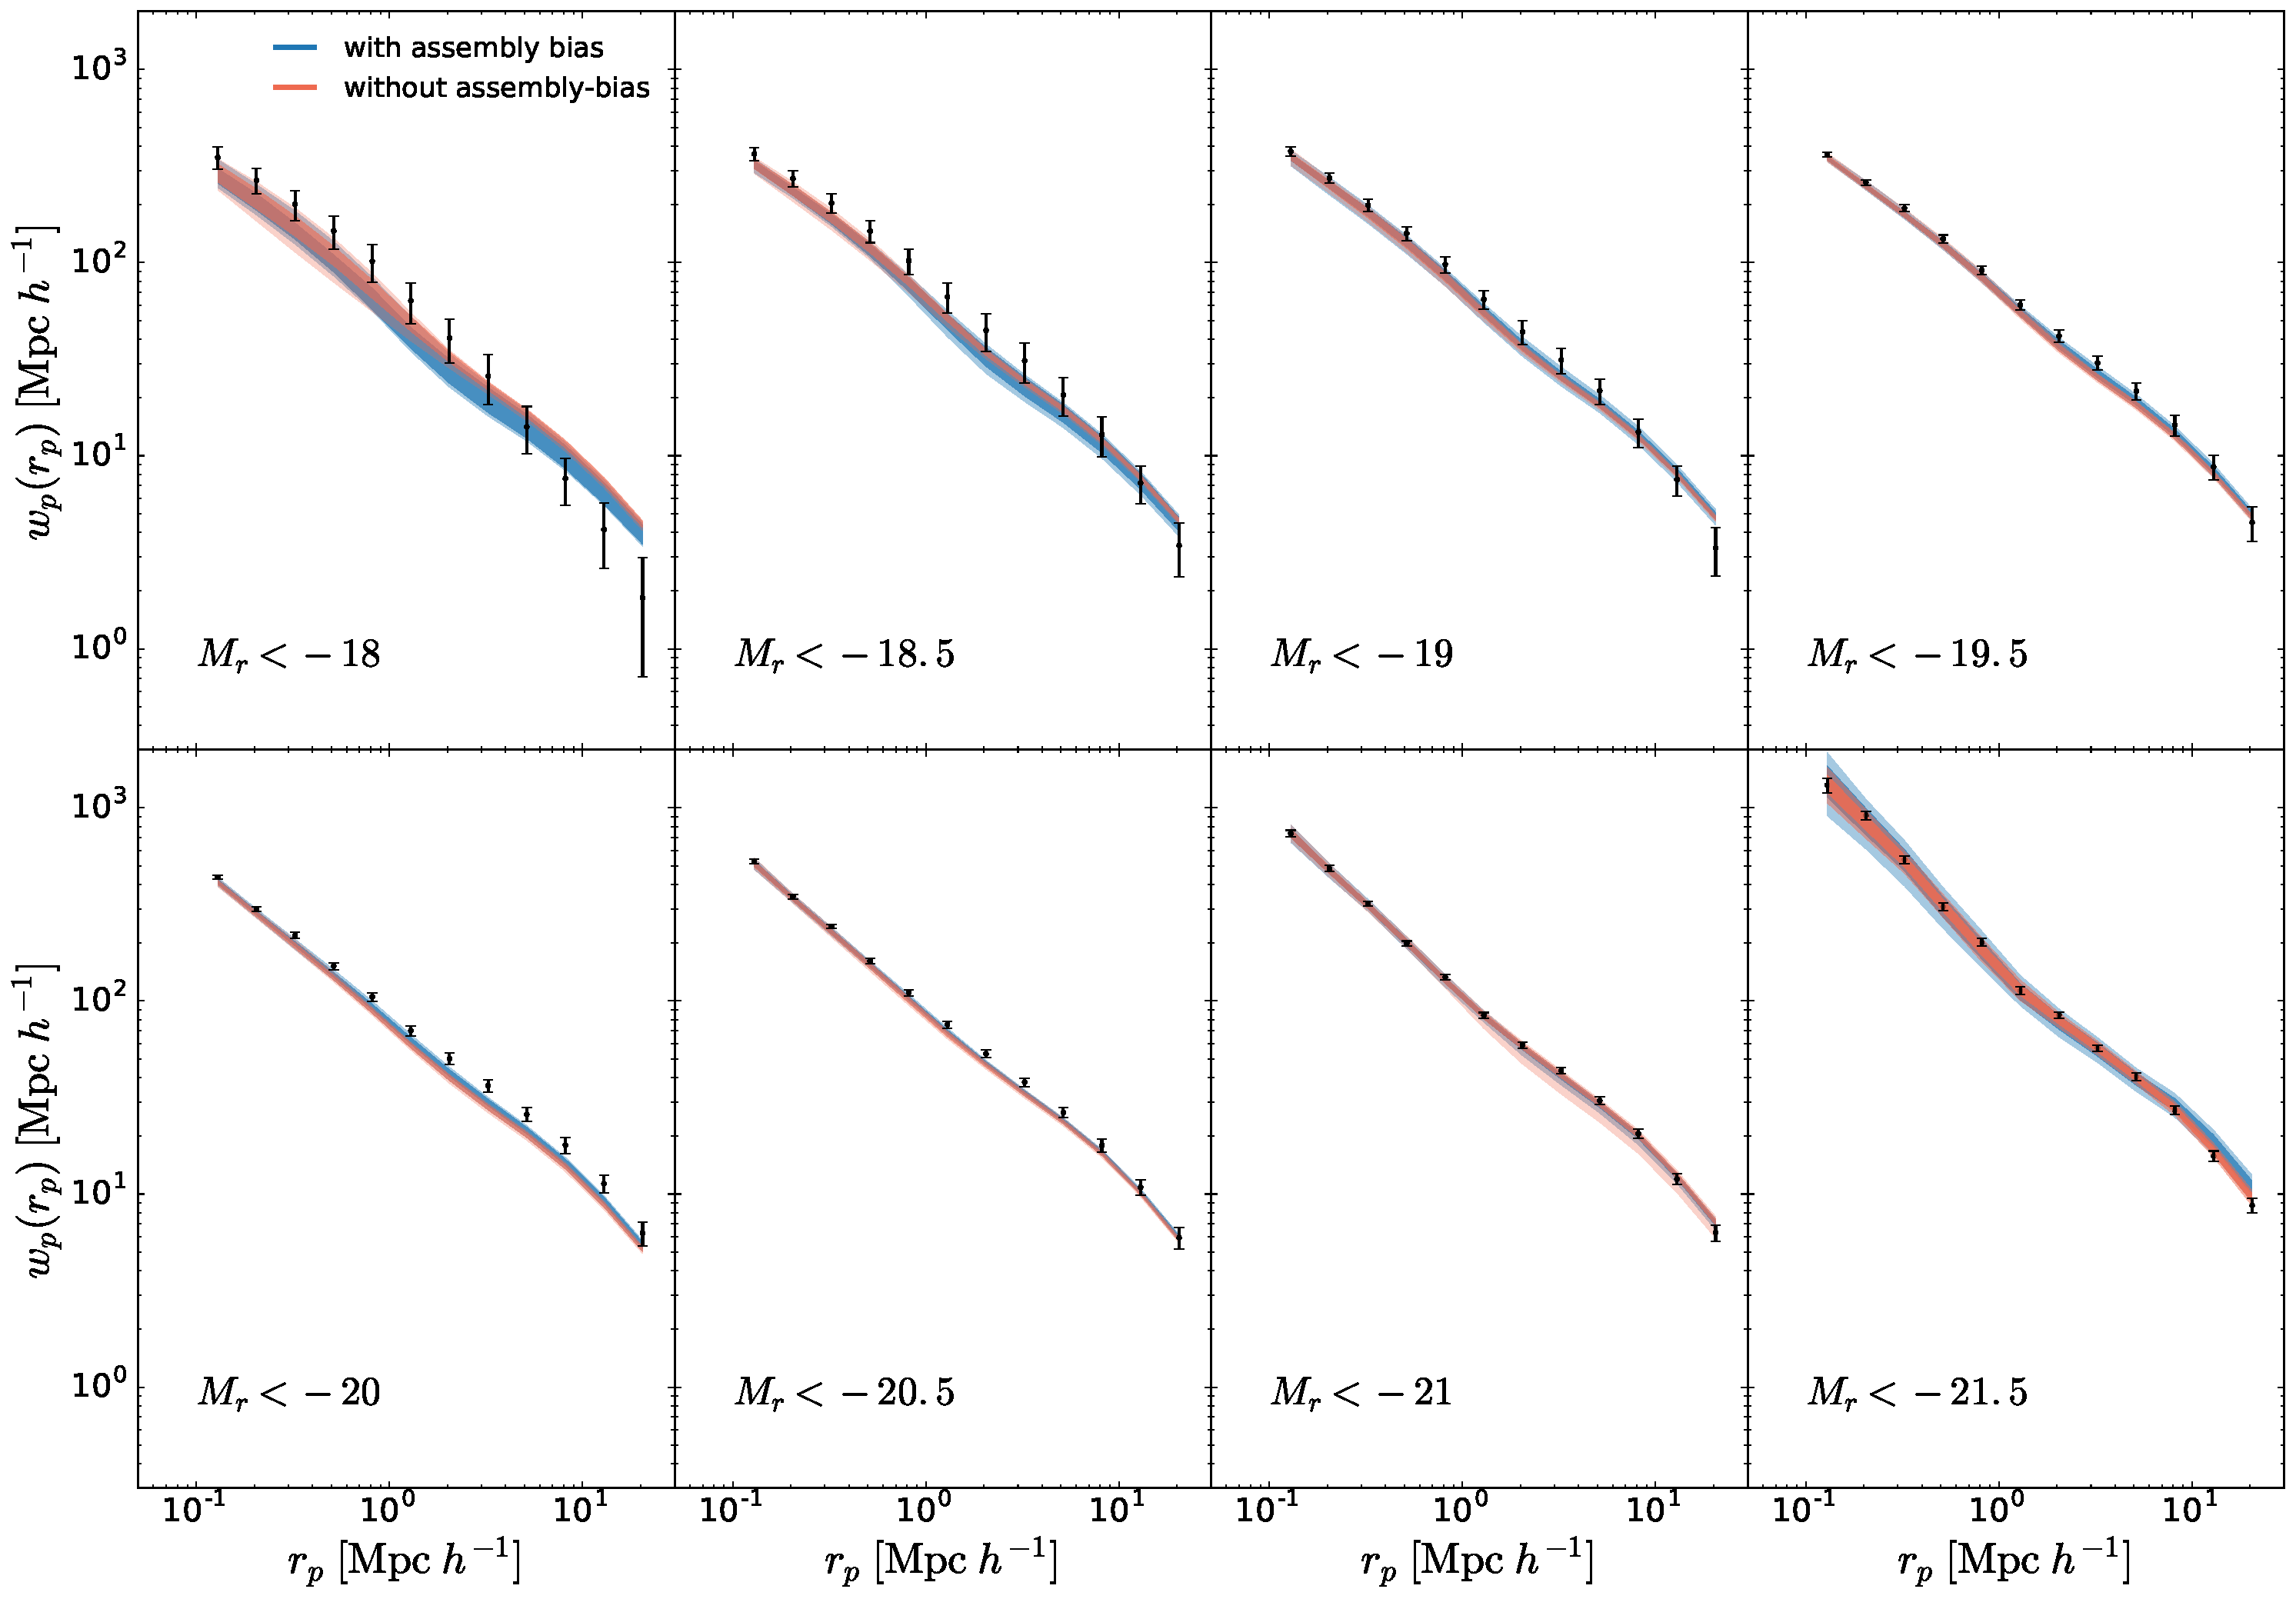
\includegraphics[width=\textwidth]{figures/gambly/wpmodel.pdf}
\caption{Comparison between the posterior predictions of $w_{p}(r_{p})$ and the SDSS $w_{p}(r_{p}$ measurements. Predictions from the standard HOD model (HOD model with assembly bias) are shown in red (blue). The Dark and light shaded regions mark the 68$\%$ and the 95$\%$ confidence intervals. The errorbars are from the diagonal elements of the covariance matrix.}
\label{fig:wpmodel}
\end{center}
\end{figure*}
%\clearpage
%%%%%%%%%%%%%%%%%%%%%%%%%%%%%%%%%%%%%%%%%%%%%%%%%%%%%%%%
% WPRES
%%%%%%%%%%%%%%%%%%%%%%%%%%%%%%%%%%%%%%%%%%%%%%%%%%%%%%%%
\begin{figure*}[p]~\\
\begin{center}
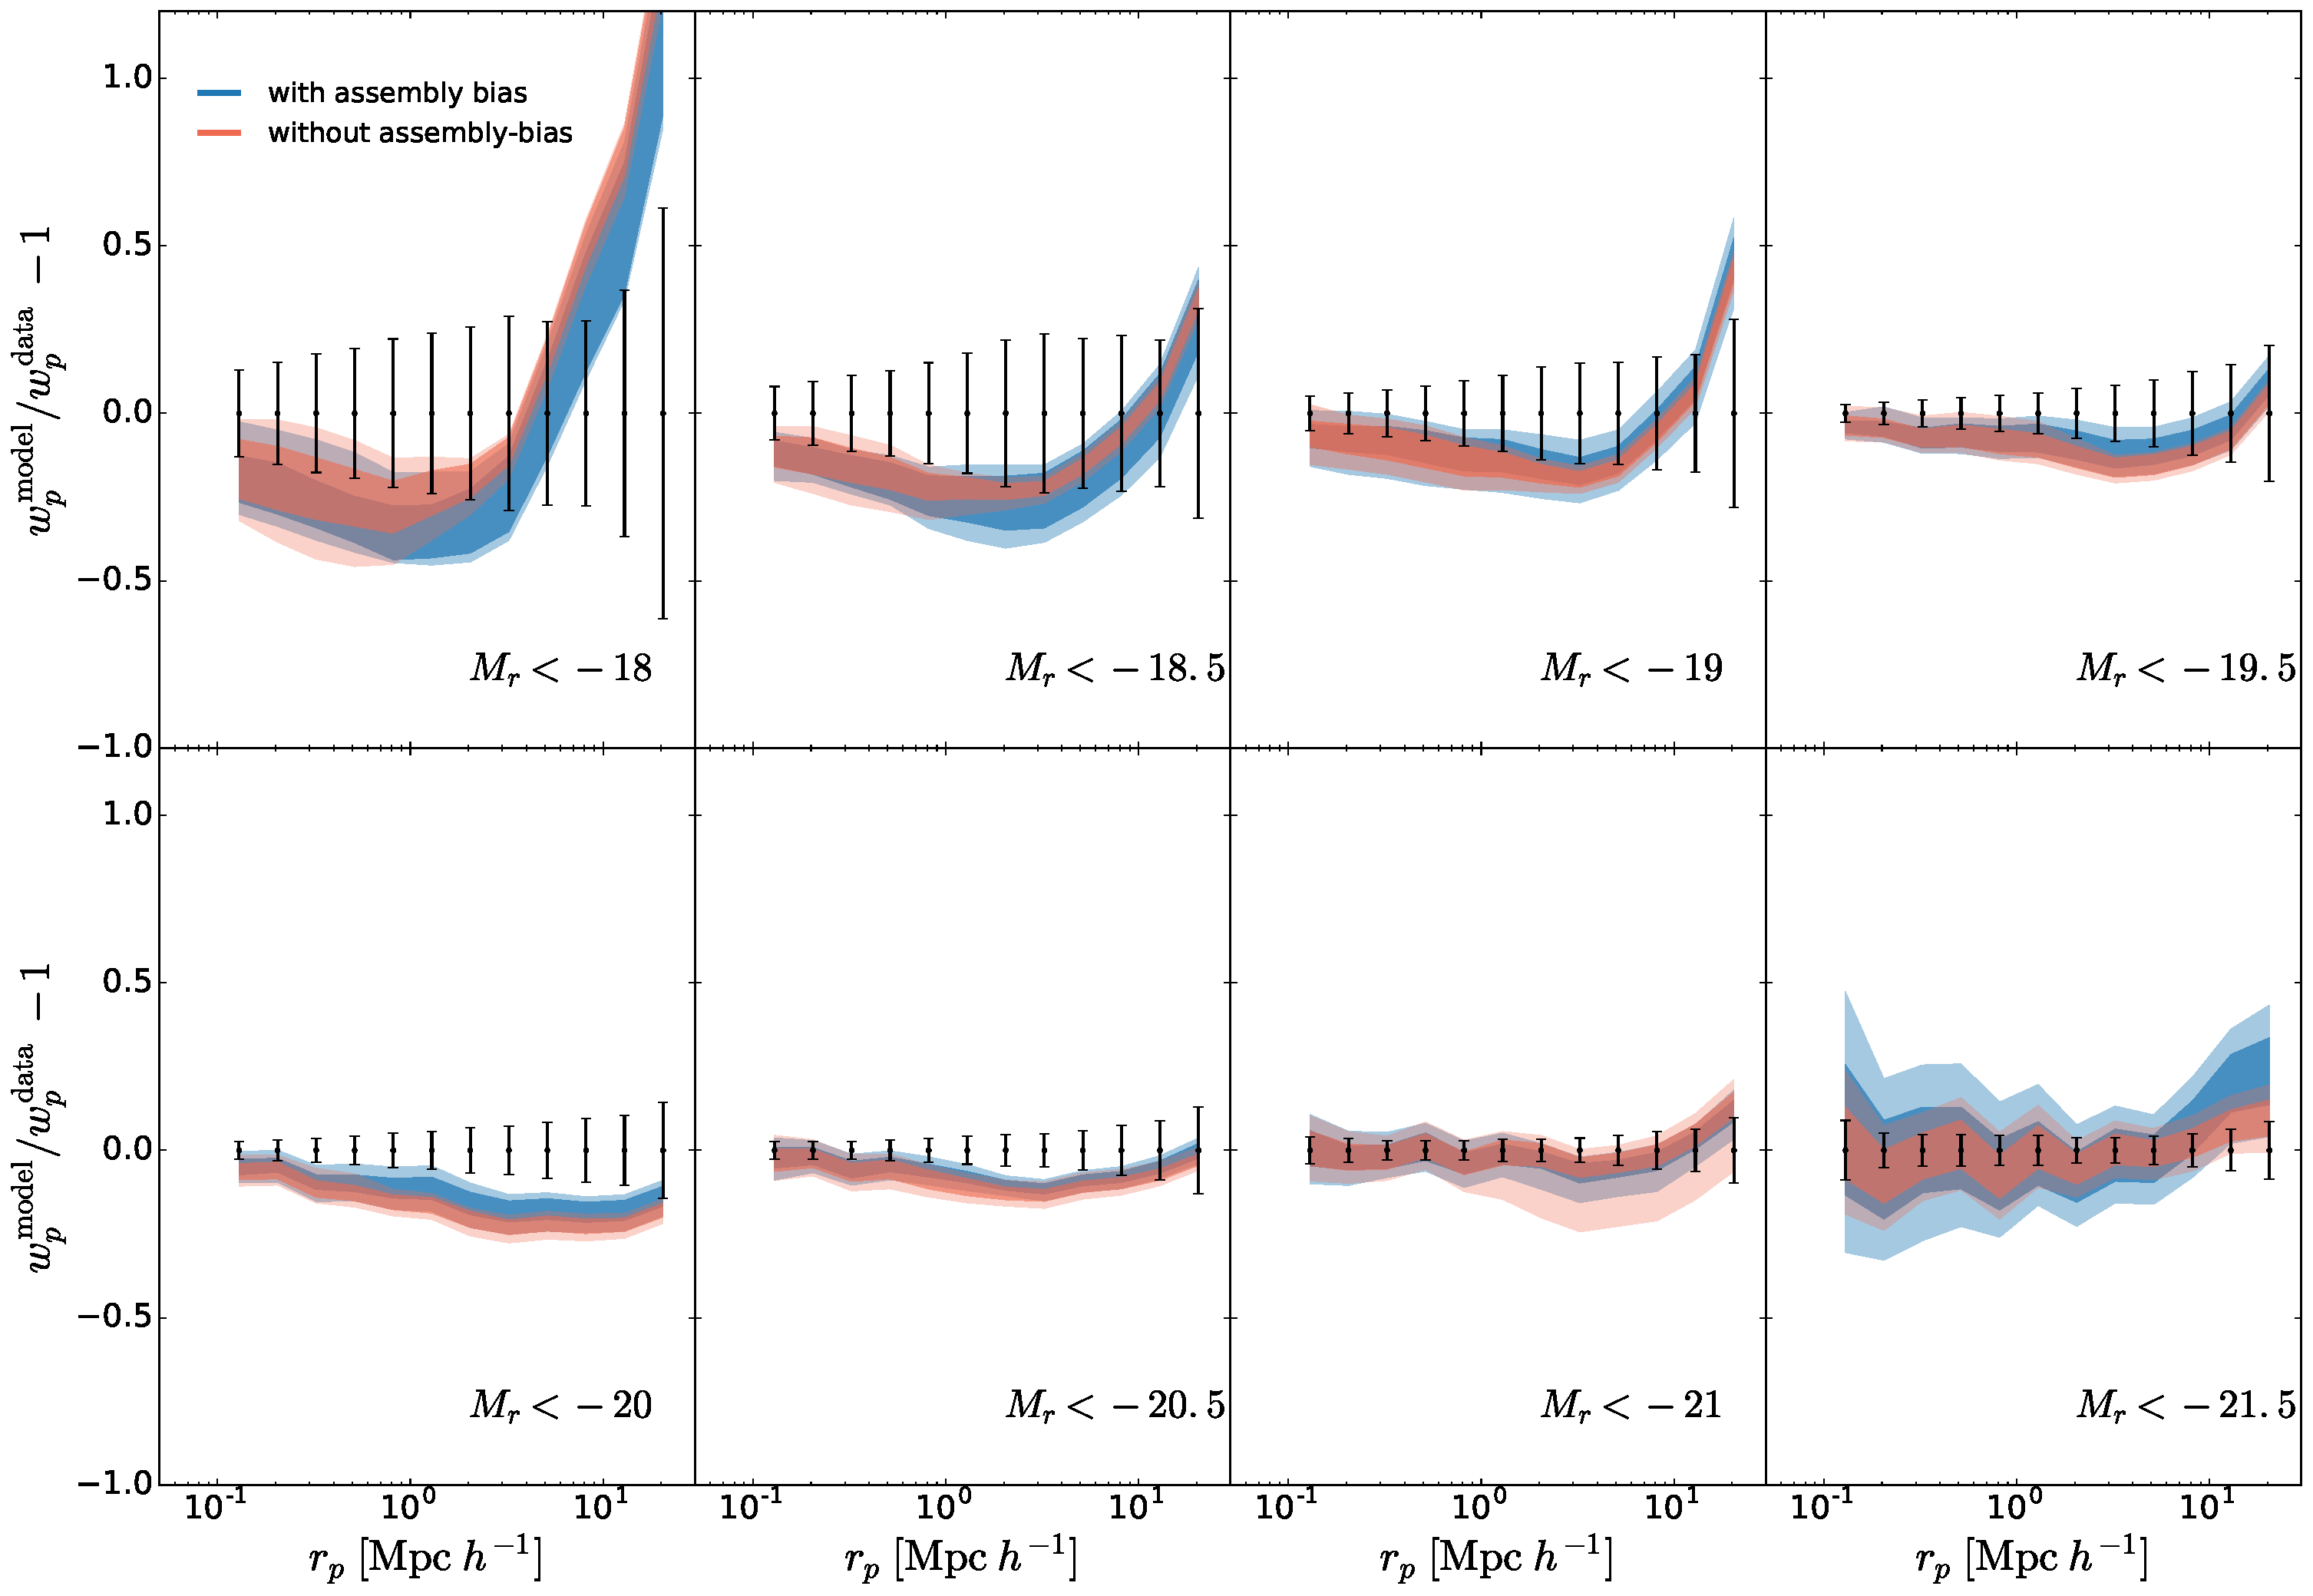
\includegraphics[width=\textwidth]{figures/gambly/wpres.pdf}
\caption{Same as Figure \ref{fig:wpmodel}, but showing the fractional difference between the posterior predictions and the observed projected 2PCF for all the luminosity threshold samples. In all luminosity threshold samples, predictions of the two models for small scale clustering are consistent. In the samples that favor more positive values of the central assembly bias parameter ($M_{\rm r}<-19.5,-19,-20,-20.5$), modeling of the intermediate and large scale clustering is slightly improved. The large scale clustering modeling of the $M_{\rm r}<-18$ sample is also improved because of negative constraints on $\acen$ which is equivalent to allocation of more central galaxies in low concentration halos at fixed halo mass.}
\label{fig:wpres}
\end{center}
\end{figure*}

%\clearpage

%%%%%%%%%%%%%%%%%%%%%%%%%%%%%%%%%%%%%%%%%%%%%%%%%%%%%%%%
% WP RANDOMIZED
%%%%%%%%%%%%%%%%%%%%%%%%%%%%%%%%%%%%%%%%%%%%%%%%%%%%%%%%
\begin{figure*}[p]~\\
\begin{center}
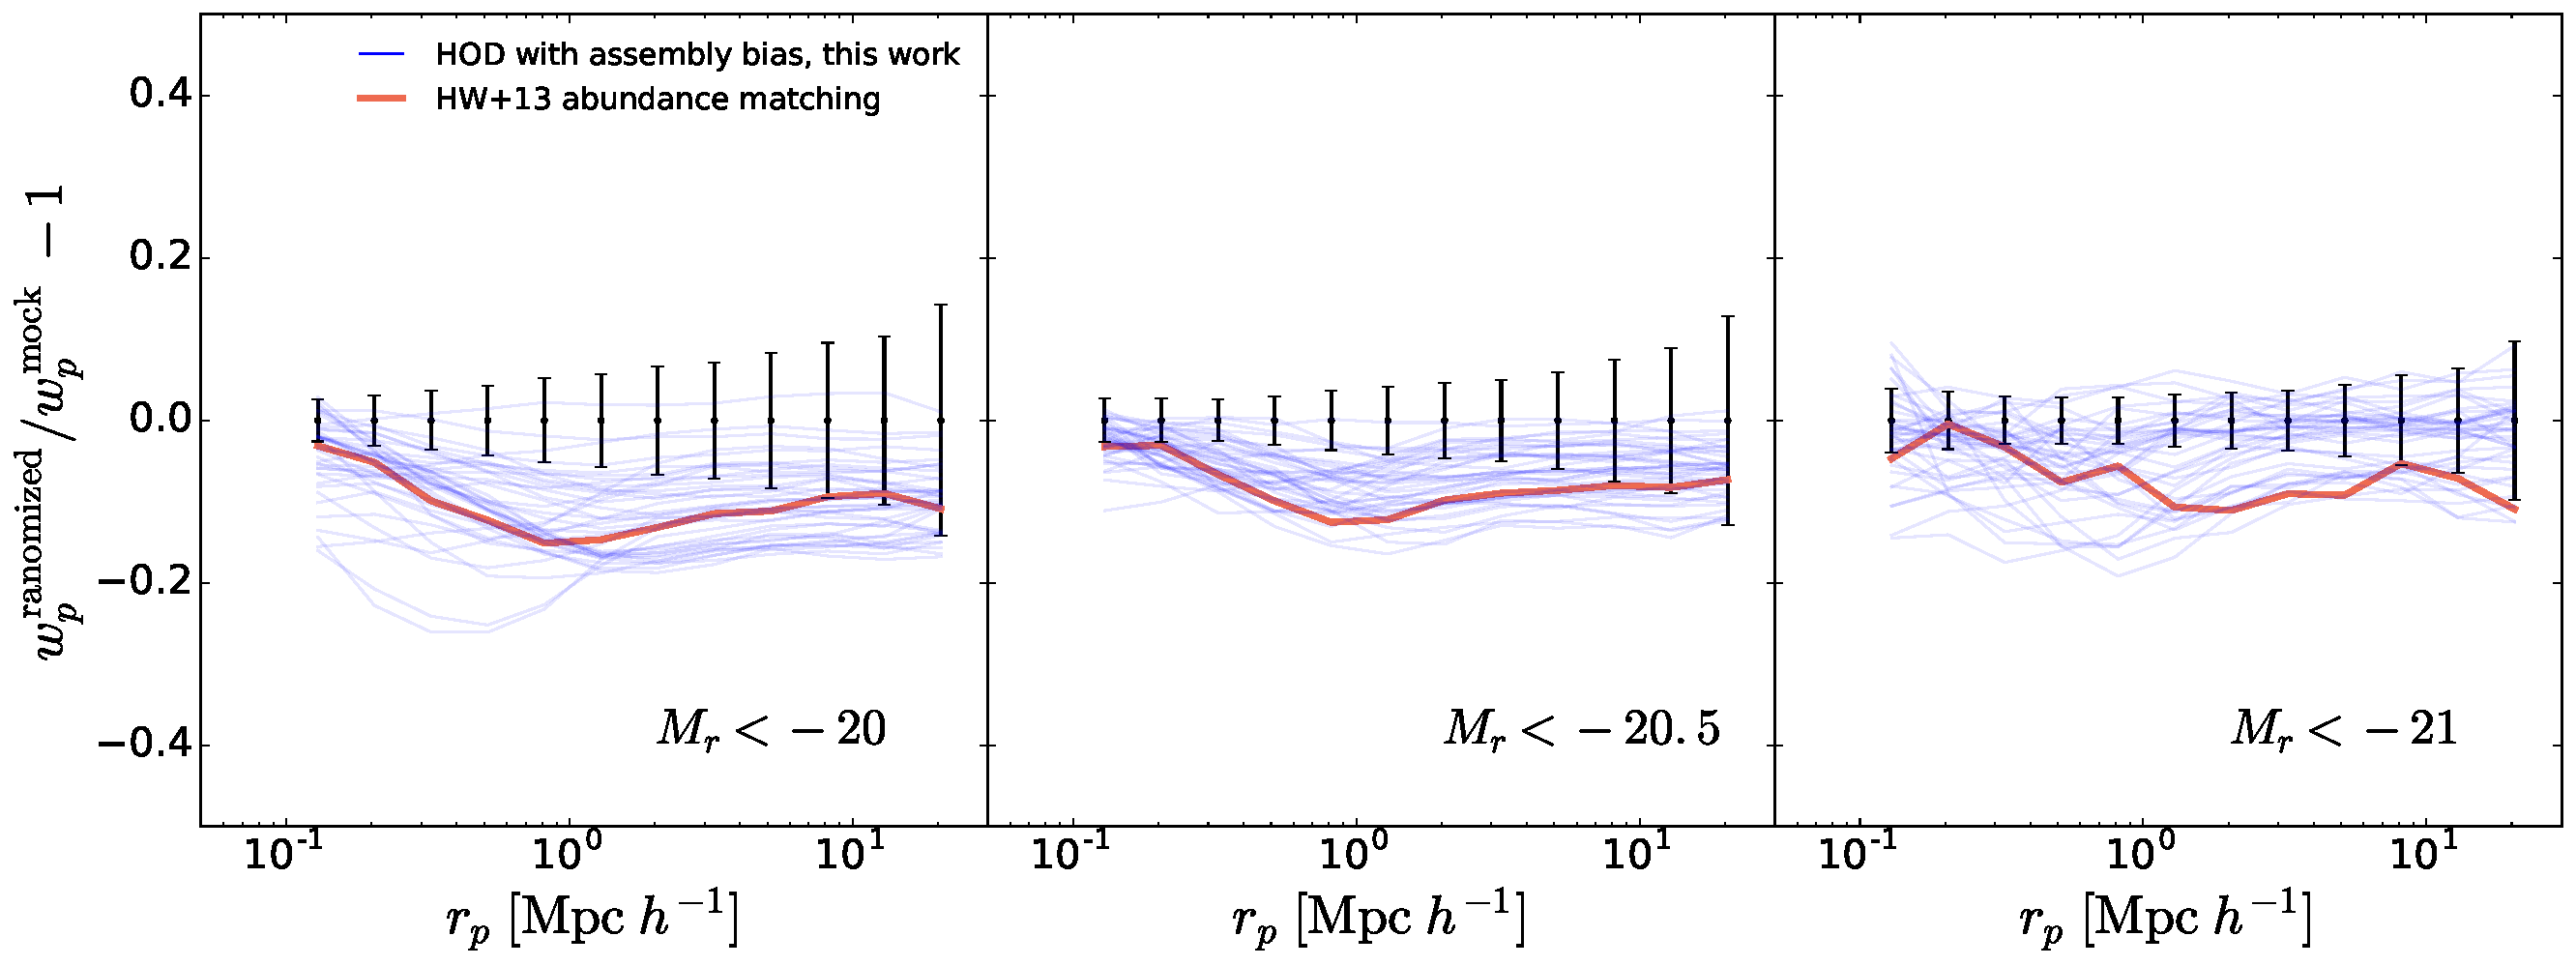
\includegraphics[width=\textwidth]{figures/gambly/paper_wprandom.pdf}
 \caption{Demonstration of the relative difference in $w_{p}$ between randomized and non-randomized catalogs for different luminosity threshold samples: $M_{\mathrm r}<-20,-20.5,-21$. The errorbars are from the diagonal elements of the covariance matrix. The blue lines correspond to the random draws from the posterior probability (summarized in Table \ref{tab:constraints}) over the parameters of the HOD model with assembly bias. The red line corresponds to the subhalo abundance matching catalog (\citealt{hw2013,hearin2014}). Our constraints favor \emph{more} \emph{moderate} levels of the impact of assembly bias on galaxy clustering than the levels seen in the abundance matching mock catalogs. Within both models, the small scale clustering remains unaltered after randomizing the catalogs, signaling the lack of correlation between the satellite occupation and the halo concentration at a fixed mass in the two models.}
\label{fig:randomized}
\end{center}
\end{figure*}

%\clearpage

%%%%%%%%%%%%%%%%%%%%%%%%%%%%%%%%%%%%%%%%%%%%%%%%%%%%%%%%
% Information Criteria
%%%%%%%%%%%%%%%%%%%%%%%%%%%%%%%%%%%%%%%%%%%%%%%%%%%%%%%%
\begin{figure*}[p]~\\
\begin{center}
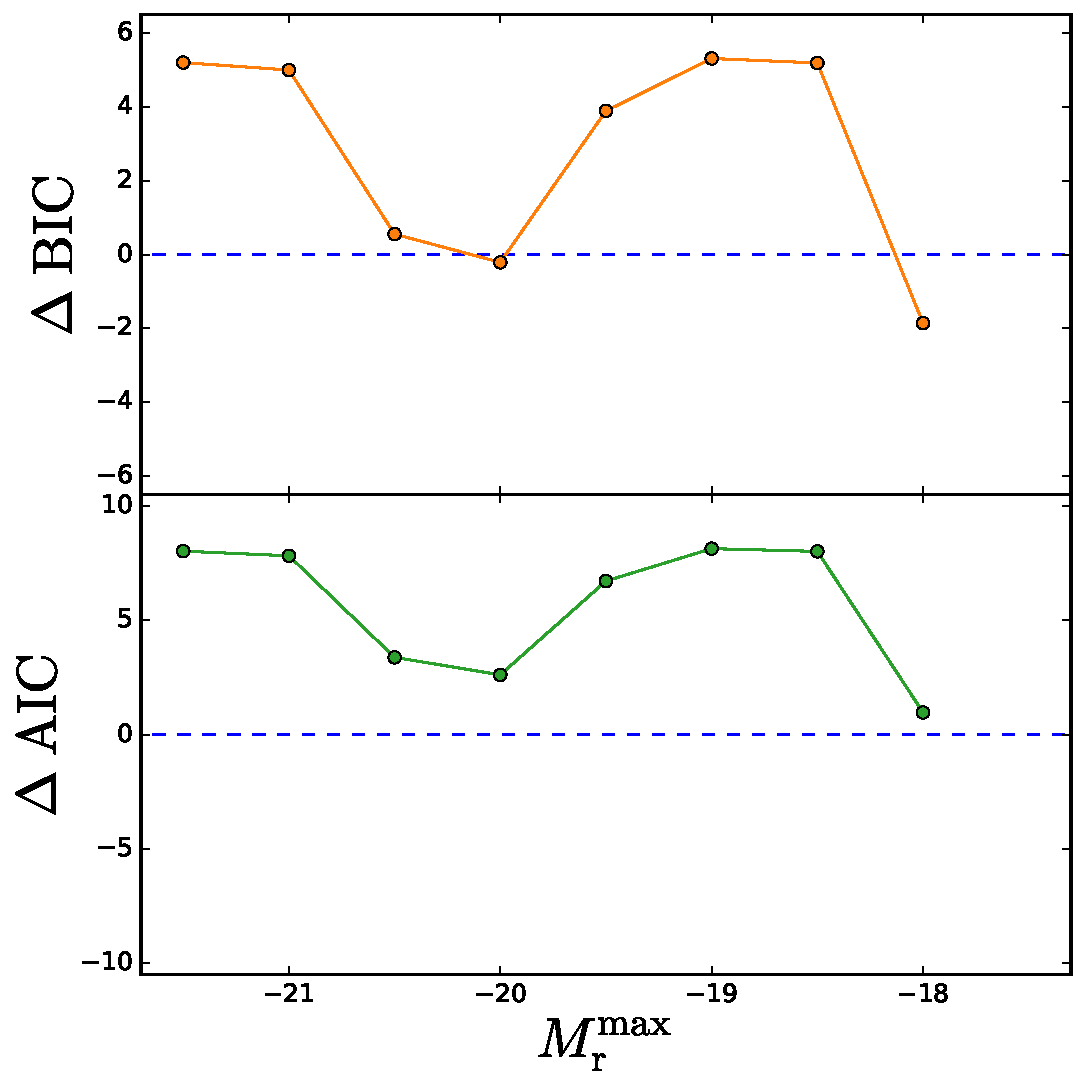
\includegraphics[width=0.8\textwidth]{figures/gambly/IC.pdf}
\caption{Difference in the information criteria between the HOD model with assembly bias and the model without assembly bias. $\bf{Top}$: $\Delta$BIC = BIC(with assembly bias) - BIC(without assembly bias). $\bf{Bottom}$: $\Delta$AIC = AIC(with assembly bias) - AIC(without assembly bias). According to BIC (AIC), the more complex model with assembly bias is favored once $\Delta$BIC$<0$ ($\Delta$AIC$<0$). Both $\Delta$BIC and $\Delta$AIC are lower for the samples with tighter constraints over the central assembly bias parameter $\acen$, with $\Delta$BIC being (marginally) negative only for $M_{\rm r}<-20,-18$ samples that yield strongest constraints on $\acen$.} 
\label{fig:ic}
\end{center}
\end{figure*}

%\clearpage

%%%%%%%%%%%%%%%%%%%%%%%%%%%%%%%%%%%%%%%%%%%%%%%%%%%%%%%%
% BIAS COMPARISON
%%%%%%%%%%%%%%%%%%%%%%%%%%%%%%%%%%%%%%%%%%%%%%%%%%%%%%%%
\begin{figure*}[p]~\\
\begin{center}
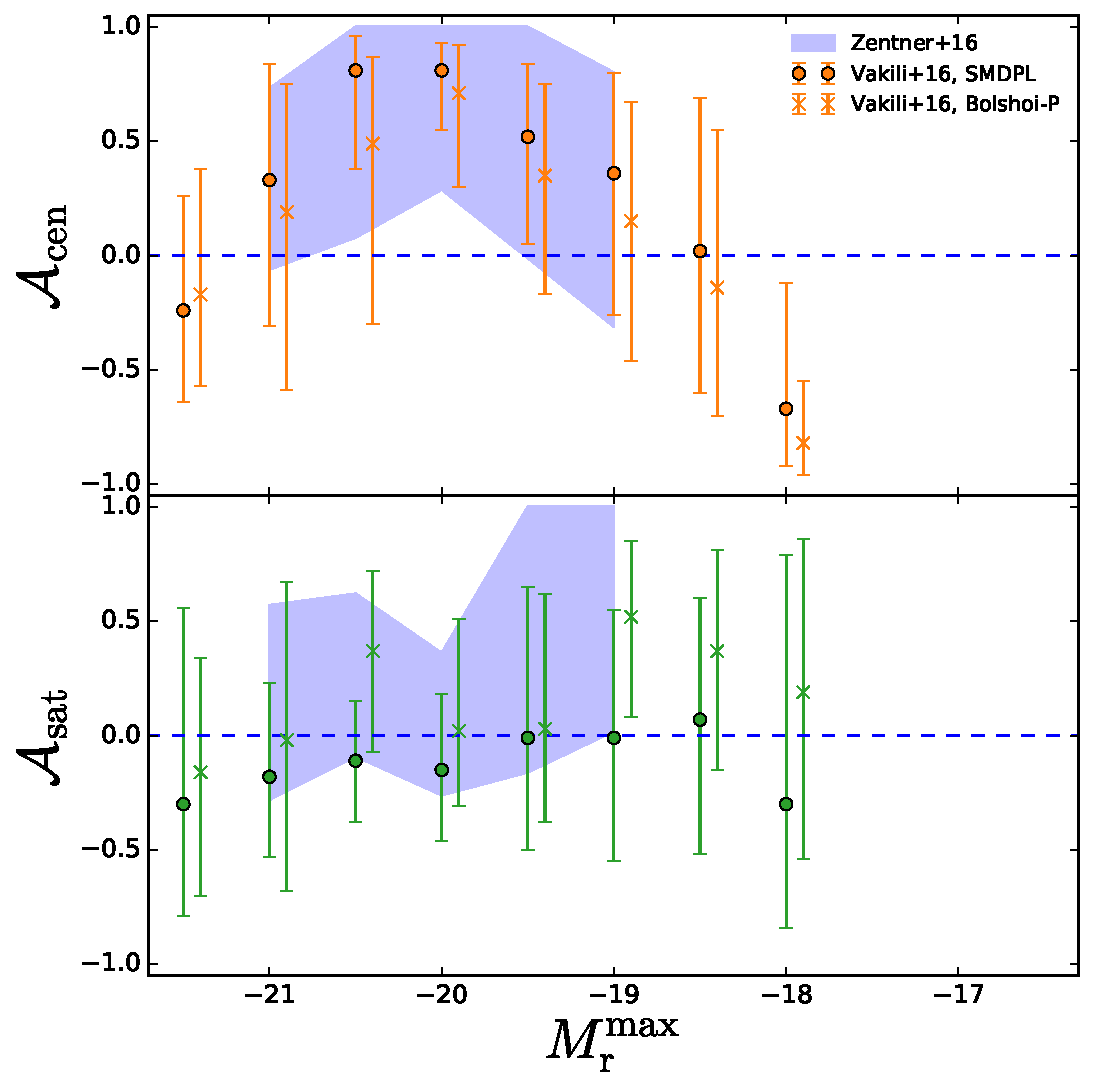
\includegraphics[width=0.8\textwidth]{figures/gambly/bias_comparison.pdf}
\caption{Comparison between the constraints on the assembly bias parameters $\acen$ (shown in the top panel) and $\asat$ (shown in the bottom panel) for different simulations: $\mathtt{SMDP}$ (shown with circle), and $\mathtt{BolshoiP}$ (shown with cross). The errorbars mark the 68$\%$ uncertainty over the parameters. Shaded blue regions show the upper and lower bounds reported by \citet{zentner2016} that uses the $\mathtt{BolshoiP}$ and clustering measurements of \citet{zehavi2011}. For the confidence intervals corresponding to the shaded blue regions, we refer the readers to Table 2 of \citet{zentner2016}. The central assembly bias constraints found from the two simulations are consistent, with the constraints for from the $\mathtt{SMDP}$ simulation being tighter for the most luminous samples. The constraints on $\asat$ from the two simulations are largely in agreement with the exception of $M_{\rm r}<-19 ,\; -20.5$ samples that favor more positive values of $\asat$ when the $\mathtt{BolshoiP}$ simulation is used.}
\label{fig:bias_comparison}
\end{center}
\end{figure*}

%\clearpage

%%%%%%%%%%%%%%%%%%%%%%%%%%%%%%%%%%%%%%%%%%%%%%%%%%%%%%%%
% ASAT DISCREPANCY
%%%%%%%%%%%%%%%%%%%%%%%%%%%%%%%%%%%%%%%%%%%%%%%%%%%%%%%%
\begin{figure*}[p]~\\
\begin{center}
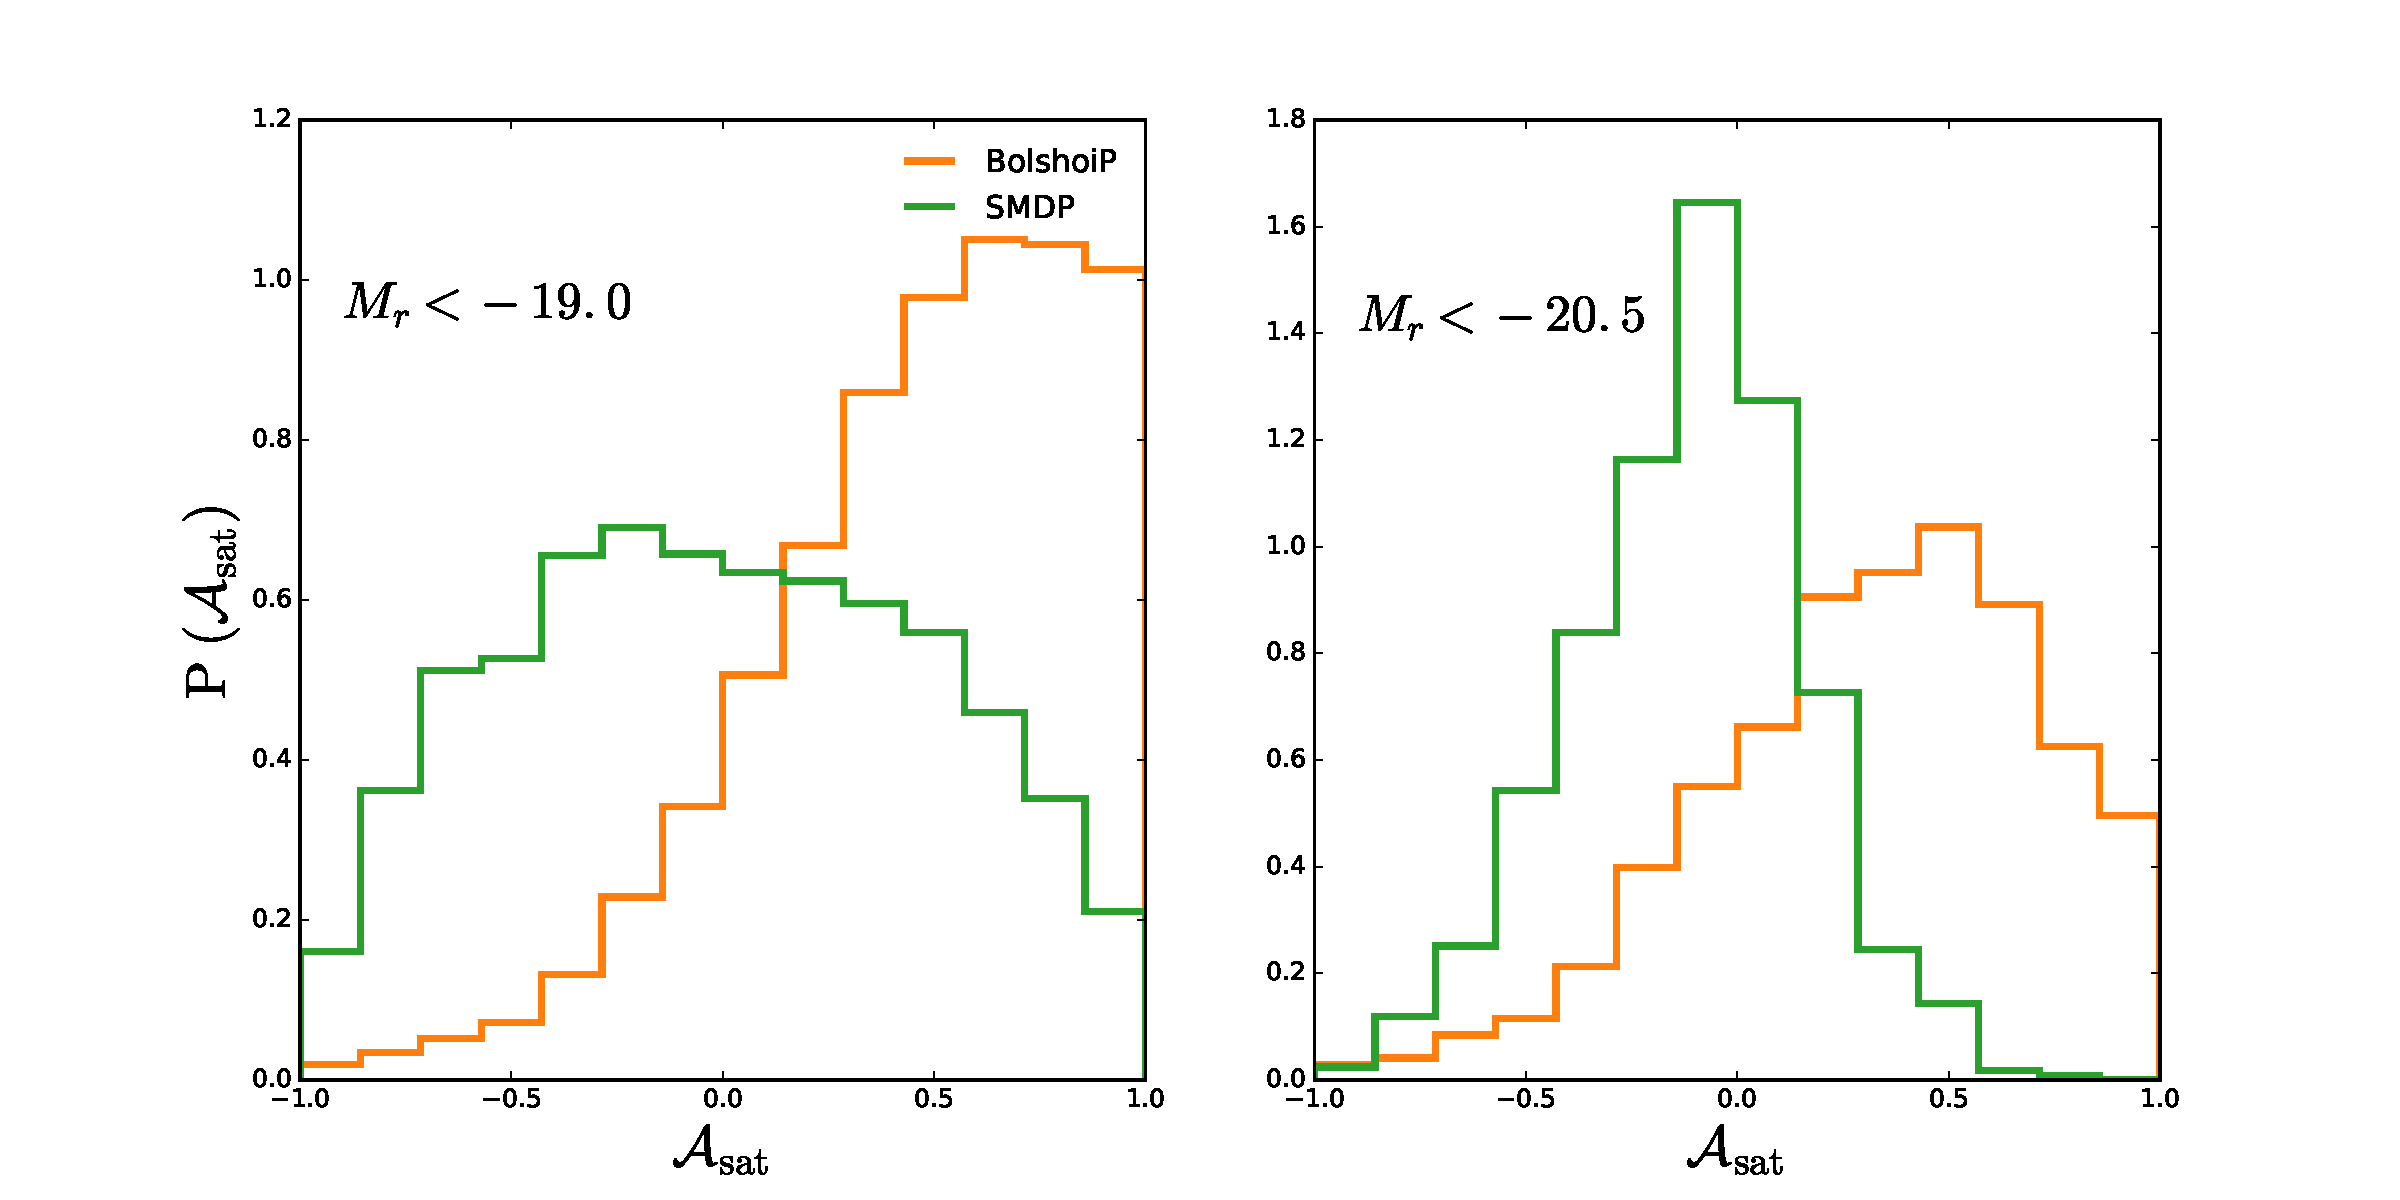
\includegraphics[width=\textwidth]{figures/gambly/hist_comparison.pdf}
\caption{Constraints over the satellite assembly bias parameters from luminosity-threshold samples $M_{\rm r}<-19 ,\; -20.5$, for two different simulations: $\mathtt{BolshoiP}$ (yellow), and $\mathtt{SMDPL}$ (green). The $\asat$ constraints found using the $\mathtt{BolshoiP}$ simulation favor more positive values of $\asat$, while the constraints found using the $\mathtt{SMDP}$ simulation favor zero satellite assembly bias.}
\label{fig:asat_comparison}
\end{center}
\end{figure*}

%\clearpage

%%%%%%%%%%%%%%%%%%%%%%%%%%%%%%%%%%%%%%%%%%%%%%%%%%%%%%%%
% EXAMPLE POSTERIOR PDF
%%%%%%%%%%%%%%%%%%%%%%%%%%%%%%%%%%%%%%%%%%%%%%%%%%%%%%%%
\begin{figure*}[p]~\\
\begin{center}
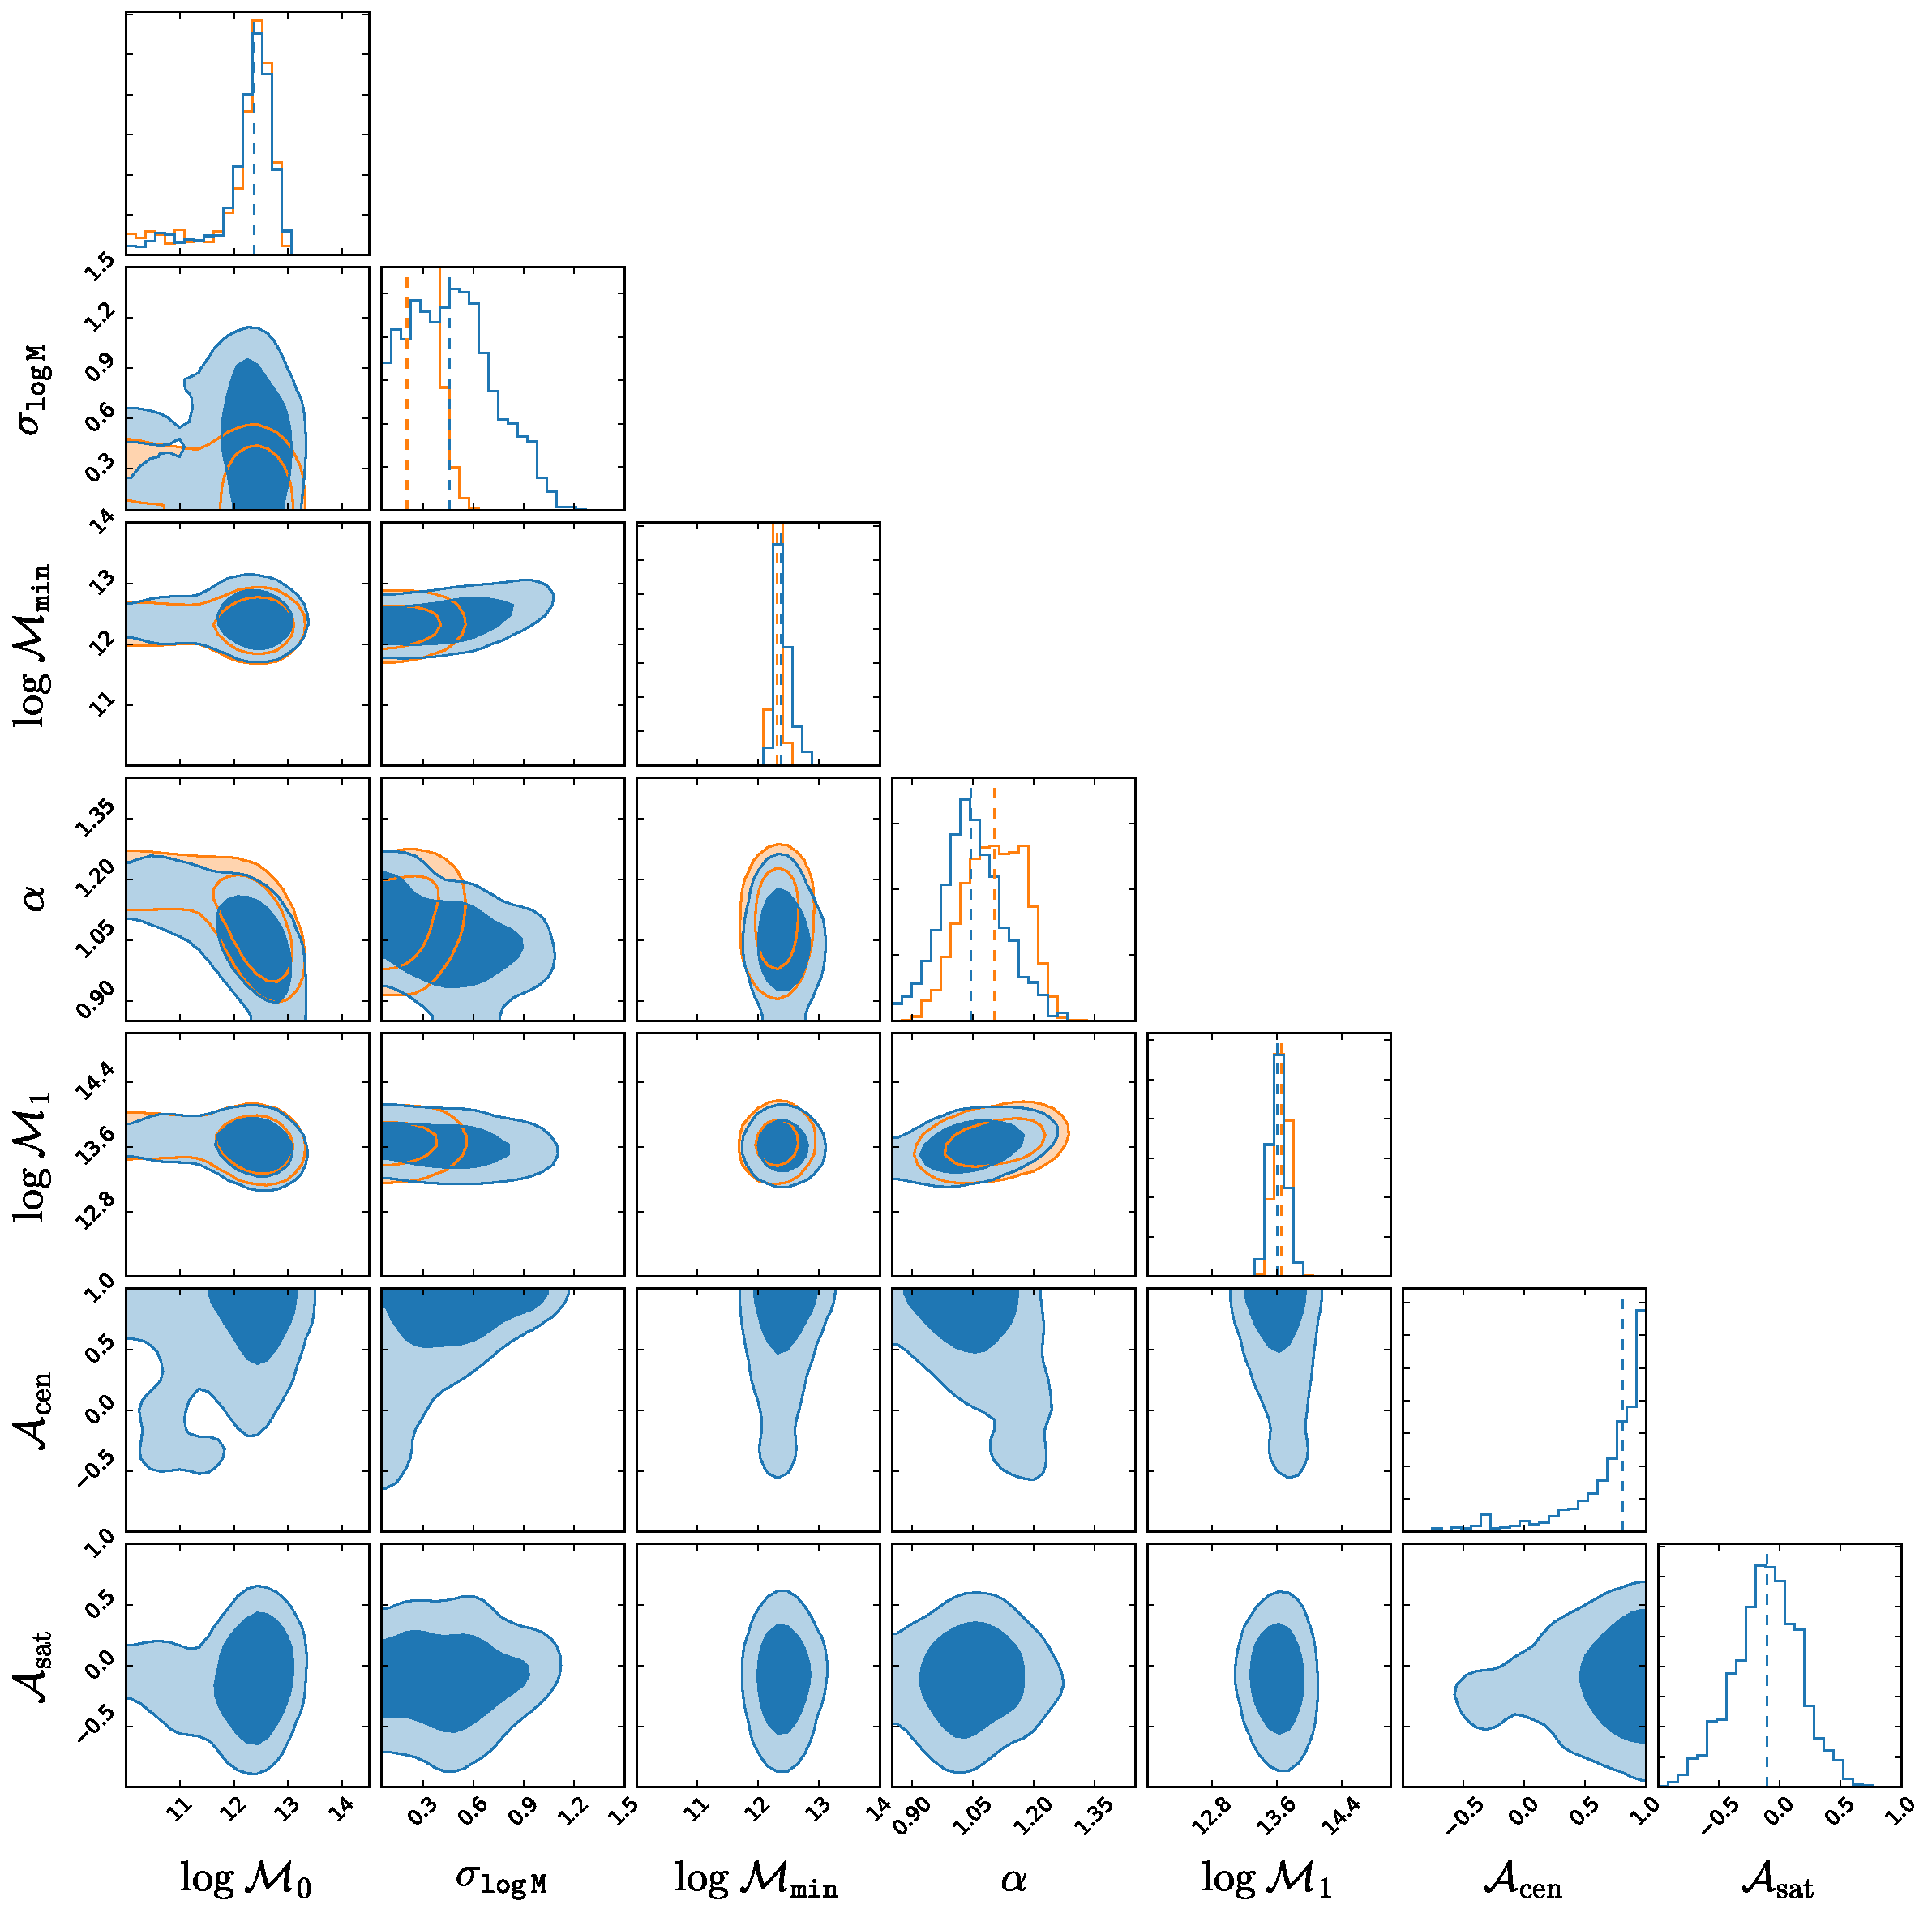
\includegraphics[width=0.9\textwidth]{figures/gambly/post20_5combined.pdf}
\caption{An example of posterior probability distribution over the parameters of the standard HOD model with no assembly bias (shown with yellow), and the HOD model with assembly bias (shown in blue). These constraints are obtained from the clustering measurements of the $M_{\rm r} < -20.5$ luminosity threshold sample. The dark (light) blue shaded regions show the 68$\%$ (95 $\%$) confidence intervals. The constraints on $\acen$ and $\asat$ show positive correlation between the central occupation and the halo concentration at fixed halo mass, and lack of correlation between the satellite occupation and halo concentration at fixed halo mass.}
\label{fig:posterior}
\end{center}
\end{figure*}

%\bibliographystyle{yahapj}
%\bibliography{assemble}



\def\pvm#1{[PM: {\it #1}] }
\def\pvm2#1{}

\newcommand{\be}{\begin{equation}}
\newcommand{\ee}{\end{equation}}
\newcommand{\ba}{\begin{eqnarray}}
\newcommand{\ea}{\end{eqnarray}}
\newcommand{\mperh}{\,h^{-1}\,{\rm Mpc}}
\newcommand{\hperm}{\,h\,{\rm Mpc}^{-1}}

% PRD specific
%\documentclass[aps,prd,showpacs,superscriptaddress,groupedaddress]{revtex4}  % twocolumn submission
%\documentclass[aps,preprint,showpacs,superscriptaddress,groupedaddress]{revtex4}  % for double-spaced preprint
%\usepackage{dcolumn}   % needed for some tables
%\usepackage{bm}        % for math
% avoids incorrect hyphenation, added Nov/08 by SSR
%\hyphenation{ALPGEN}
%\hyphenation{EVTGEN}
%\hyphenation{PYTHIA}

%\usepackage{natbib}	% For citep and citep
%\usepackage[breaklinks]{hyperref}	% for blackboard bold numbers
%\usepackage{hyperref}
%\usepackage{microtype}
%\usepackage{aas_macros}
%\usepackage{times}
%\usepackage{txfonts}
%\usepackage{url}
%\usepackage{amsmath}
%\usepackage{amsbsy}
%\usepackage{graphicx}
%\usepackage{subfig}
%\usepackage{xspace}
%\usepackage{float}
%\usepackage{caption}
%\usepackage{amsfonts}
%\usepackage{amssymb}
%\usepackage{multirow}
%\usepackage{color}	
%\usepackage[breaklinks, colorlinks, citecolor=blue, linkcolor=black, urlcolor=black]{hyperref}%with colors
%\usepackage{hyperref}%without colors
%\input{macros.tex}
%\newcommand{\todo}[1]{\textcolor{blue}{[TODO: #1]}}
%\newcommand{\bl}[1]{\textcolor{blue}{[BL: #1]}}
%\newcommand{\dwh}[1]{\textcolor{cyan}{[DWH: #1]}}

\chapter{Accurate galaxy-halo mocks with automatic bias estimation and particle-mesh gravity solvers\chaplabel{mocks}}

This \paper\ is joint work with Francisco-Shu~Kitaura (IAC), Yu~Feng (Berkeley),  Gustavo~Yepes (UAM), Cheng~Zhao (Tsinghua), Chia-Hsun~Chuang (Leibniz), ChangHoon~Hahn (NYU) and it is submitted to the \emph{Monthly Royal Astronomical Society Notice}.


\section{abstract}
Reliable extraction of cosmological information from clustering measurements of galaxy surveys requires estimation of the error covariance matrices of observables. The accuracy of covariance matrices is limited by our ability to generate sufficiently large number of independent mock catalogs that can describe the physics of galaxy clustering across a wide range of scales. 
Furthermore, galaxy mock catalogs are required to study systematics in galaxy surveys and to test analysis tools.
In this investigation, we present a fast and accurate approach for generation of mock catalogs for the upcoming galaxy surveys. 
Our method relies on low-resolution approximate gravity solvers to simulate the large scale dark matter field, which we then populate with halos according to a flexible nonlinear and stochastic bias model. 
In particular, we extend the \textsc{patchy} code with an efficient particle mesh algorithm to simulate the dark matter field (the \textsc{FastPM} code), and with an efficient and robust MCMC method relying on the \textsc{emcee} code for constraining the parameters of the bias model. 
Using the halos in the BigMultiDark high-resolution $N$-body simulation as a reference catalog, we demonstrate that our technique can model the bivariate probability distribution function, power spectrum, and bispectrum of halos in the reference catalog. Specifically, we show that the new ingredients permit us to reach percentage accuracy in the power spectrum up to $k\sim 0.4\; \hperm$ (within 5\% up to $k\sim 0.6\; \hperm$) with accurate bispectra improving previous results based on Lagrangian perturbation theory.

\section{Introduction}

The current and the next generation of galaxy surveys such as \textsc{eBOSS}\footnote{\url{http://www.sdss.org/surveys/eboss/}} (Extended Baryon Oscillation Spectroscopic Survey, \citealt{eBOSS}), \textsc{DESI}\footnote{\url{http://desi.lbl.gov/}} (Dark Energy Spectroscopic Instrument, \citealt{desi}), \textsc{EUCLID}\footnote{\url{http://www.euclid-ec.org/}} (\citealt{euclid}), \textsc{LSST}\footnote{\url{http://www.lsst.org/}} (\citealt{lsst}), and \textsc{WFIRST}\footnote{\url{https://www.nasa.gov/wfirst}} (\citealt{wfirst}) are expected to achieve unprecedented constraints on the cosmological parameters, growth of structure, expansion history of the universe, and modified theories of gravity. Accurate cosmological inferences with these surveys requires accurate computation of the likelihood function of the observed data given a cosmological model. This goal can be achieved provided that the uncertainties, in the form of error covariance matrices in the likelihood functions, are reliably estimated. Therefore, covariance matrices are essential ingredients in extraction of cosmological information from the data.

The most commonly used technique in estimation of the covariance matrix for galaxy clustering observables requires generation of a large number of simulated galaxy mock catalogs. These mock catalogs need to reproduce the cosmic volume probed by the galaxy surveys. They also need to describe the clustering observables with high accuracy in a wide range of scales. It has been demonstrated that both the precision and the accuracy of constraints on the cosmological parameters, regardless of the details of a given galaxy survey, depend on the number of realizations of the survey (\citealt{dodelson2013,taylor2014}). The requirement on the number of independent realizations of the survey becomes more stringent as the number of data points in a given analysis grows (\citealt{taylor2013}).
The most pressing challenges ahead of simulating a large number of catalogs are: simulation of large volumes for sampling the Baryonic Acoustic feature in the galaxy clustering, accurate description of the clustering signal at small scales, accurate clustering not only at the level of two-point statistics but also at the level of higher order statistics.  and resolving low mass halos that host fainter galaxy samples.  

High-resolution $N$-body simulations are ideal venues for reproducing the dark matter clustering accurately. But production of a large number of density field realizations with $N$-body simulations is not computationally feasible. In order to alleviate the computational cost of $N$-body simulations, several methods based on approximate gravity solvers have been introduced. Methods based on higher order Lagrangian perturbation theory (\citealt{buchert1993,bouchet1995,catelan1995,monaco2002,scocci2002,alpt}), Zeldovich approximation (\citealt{eazymock}), and approximate $N$-body simulations (\citealt{cola2013,qpm,howlet2015,cola,fastpm,ice_cola,koda}) have been demonstrated to be promising for fast generation of dark matter density field. Sampling the structures such as galaxies and halos from the dark matter density field requires an additional step. Identification of virialized regions of matter overdensity is either done through a biasing scheme (\citealt{kitaura2014,qpm}) or is done through application of friends-of-friend algorithm (\citealt{pthalo,koda,fastpm}). Methods that employ a biasing scheme need to be calibrated such that they are statistically consistent with accurate $N$-body simulations or observations. 

The \textsc{patchy} method (\citealt{kitaura2014,kitaura2015}) produces mock catalogs by first generating dark matter field with Lagrangian Perturbation Theory modified with spherical collapse model on small scales ($r \leq 2 \; \mperh$) and then sampling galaxies (halos) from the density field using nonlinear stochastic biasing introduced in \citet{kitaura2014}. This method has been shown to reproduce the two-point clustering down to $k \sim 0.3 \; \hperm$ and the counts-in-cell of the massive halos in an accurate $N$-body simulation. \citet{kitaura2015} demonstrate that the mock catalogs generated using this technique are capable of accurately describing the halo bispectrum in the reference $N$-body simulations. Furthermore, \citet{kitaura2016} used this method for massive production of mock catalogs for the cosmological analysis of the completed SDSS III Baryon Oscillation Spectroscopic Survey DR12 galaxy sample. 

Alternatively, computation of error covariance matrices can be delivered with analytical models (\citealt{feldman1994,smith2008,crocce2011,sun2013,grieb2016,klaus2016}). 
These methods are promising, though still need further investigation especially including sysytematic effects, such as the survey geometry. They will potentially permit us to use a smaller number of mock catalogs to obtain accurate covariance matrices.

In recent years, development of the shrinkage methods (\citealt{ledoit2004,pope2008,ledoit2012,joachimi2016,simpson2016}) have been shown to be promising for alleviating the requirement on the number of mocks. In principle, one could use a combination of the shrinkage methods and a smaller number of mock catalogs to reach the same level of accuracy needed for large scale structure inferences.    

Moreover, production of mocks will be a useful tool for investigation of possible sources of systematic errors as well as verification of covariance matrices derived from analytical methods.

In this investigation, we introduce an MCMC method for calibration of the bias model of the \textsc{patchy} code. This method constrains the bias parameters by the halo power spectrum and the halo counts-in-cells (hereafter halo PDF) of a  reference halo catalog constructed from an accurate $N$-body simulation. 

Furthermore, we replace the dark matter gravity solver of the code with the fast particle-mesh approximate $N$-body solver implemented in the \textsc{FastPM} code (\citealt{fastpm}). The advantage of the \textsc{FastPM} algorithm over other methods based on particle-mesh is its low memory requirements as well as accurate large scale growth. In addition, the dark matter density field produced by the \textsc{FastPM} code yields better nonlinear clustering than that of the perturbation theory. 

As a proof of concept, we make use of the halos in the BigMultiDark Planck high-resolution $N$-body simulation (\citealt{multidark}). This catalog has been extensively used for validation, comparison and production of galaxy mock catalogs (\citealt{chuang2015,zhao2015,kitaura2016,sergio2016}). 
In addition, we will make a statistical comparison between our \textsc{patchy} mocks and the reference catalog. We present the number density, halo PDF, and halo two-point statistics. 
We also present our results in terms of the three-point statistics since it is rising as a major complementary approach in various large-scale structure analyses \citep{slepian2015,gill2015a,gill2015b,guo2016,slepian2016a,slepian2016b,gill2017}. 


The remainder of this paper is structured as follows: In section \S \ref{sec:mockmethod}, we present our method for generating and calibrating mock catalogs. This includes description of the structure formation model, nonlinear stochastic bias model of the \textsc{patchy} code, and our MCMC method for constraining the bias parameters. We illustrate the performances using a reference halo catalog constructed from an accurate $N$-body simulation in section \S \ref{sec:mocktest}, and we discuss the main results and present our conclusions in section \S \ref{sec:mockdiscussion}.

%%%%%%%%%%%%%%%%%%%%%%%%%%%%%%%%%%%%%%
\section{Methodology}
\label{sec:mockmethod}

Our method consists of producing the large scale dark matter field on a mesh and then populating it with halos (or galaxies) with a given bias model. The parameters of that bias model are constrained with a reference catalog in an automatic statistical way. 
Our approach is agnostic about the method used for identification of halos in the reference catalog. The \textsc{patchy} code permits us to sample galaxies directly from the density field. For instance \citet{kitaura2016} samples mock galaxy catalogs based on an accurate reference mock galaxy catalog \citep{sergio2016}. 
Let us first describe in \S \ref{sec:sf} the new implementation of the structure formation in \textsc{patchy}, followed in \S \ref{sec:bias} by the bias model, and finally in  \S \ref{sec:mcmc} our novel MCMC sampling procedure to obtain the bias parameters. 

\begin{figure*}
 \begin{tabular}{ccc}
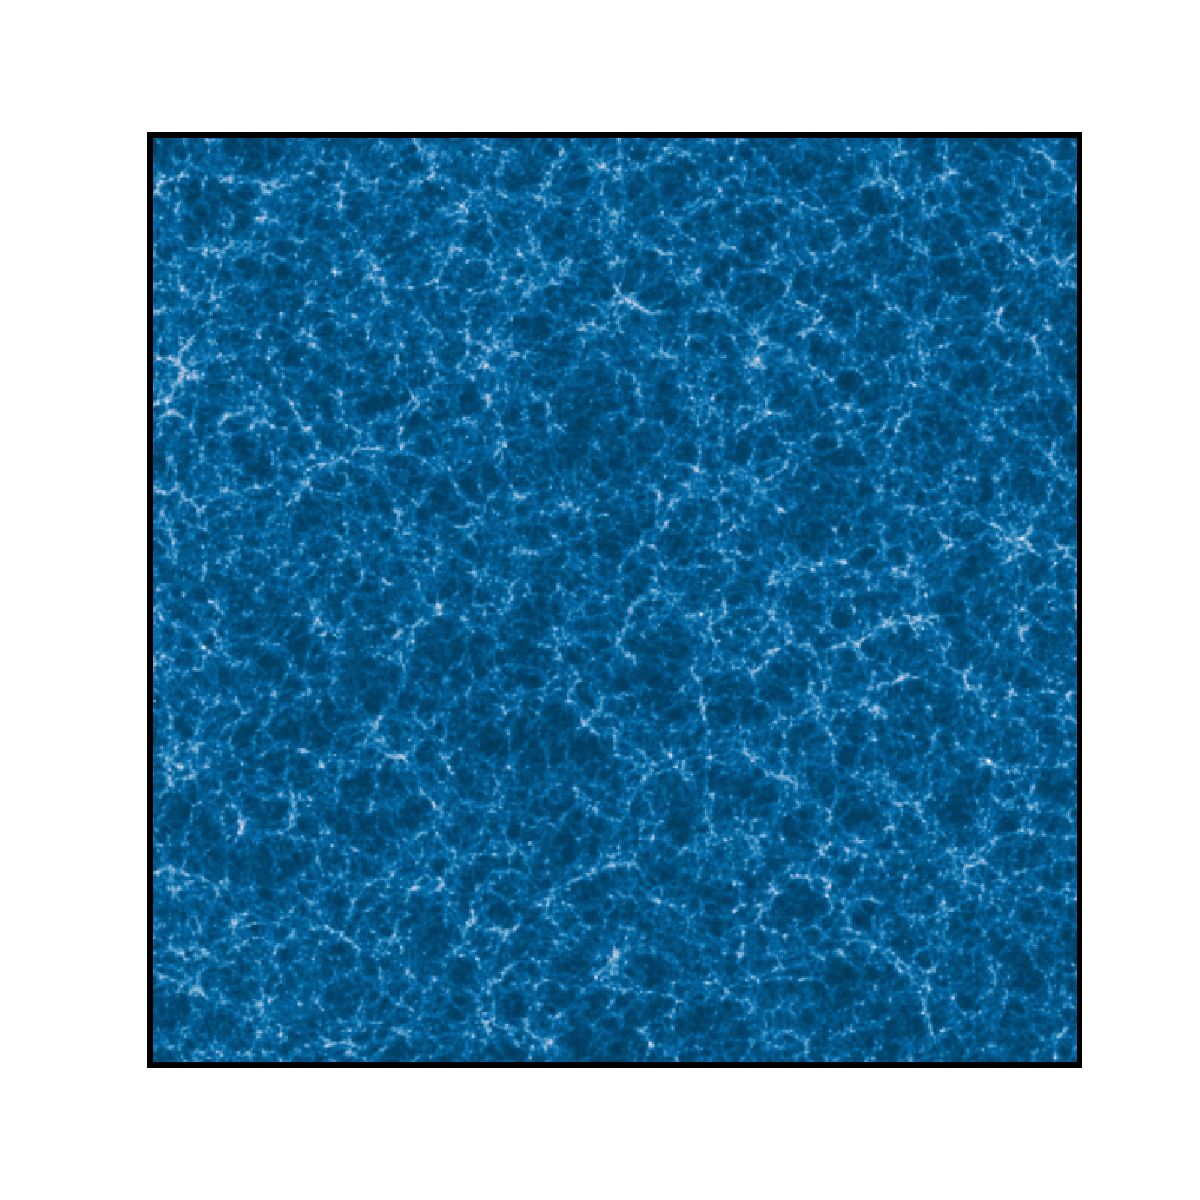
\includegraphics[width=0.3\textwidth]{figures/mocks/bigmd_large.pdf}
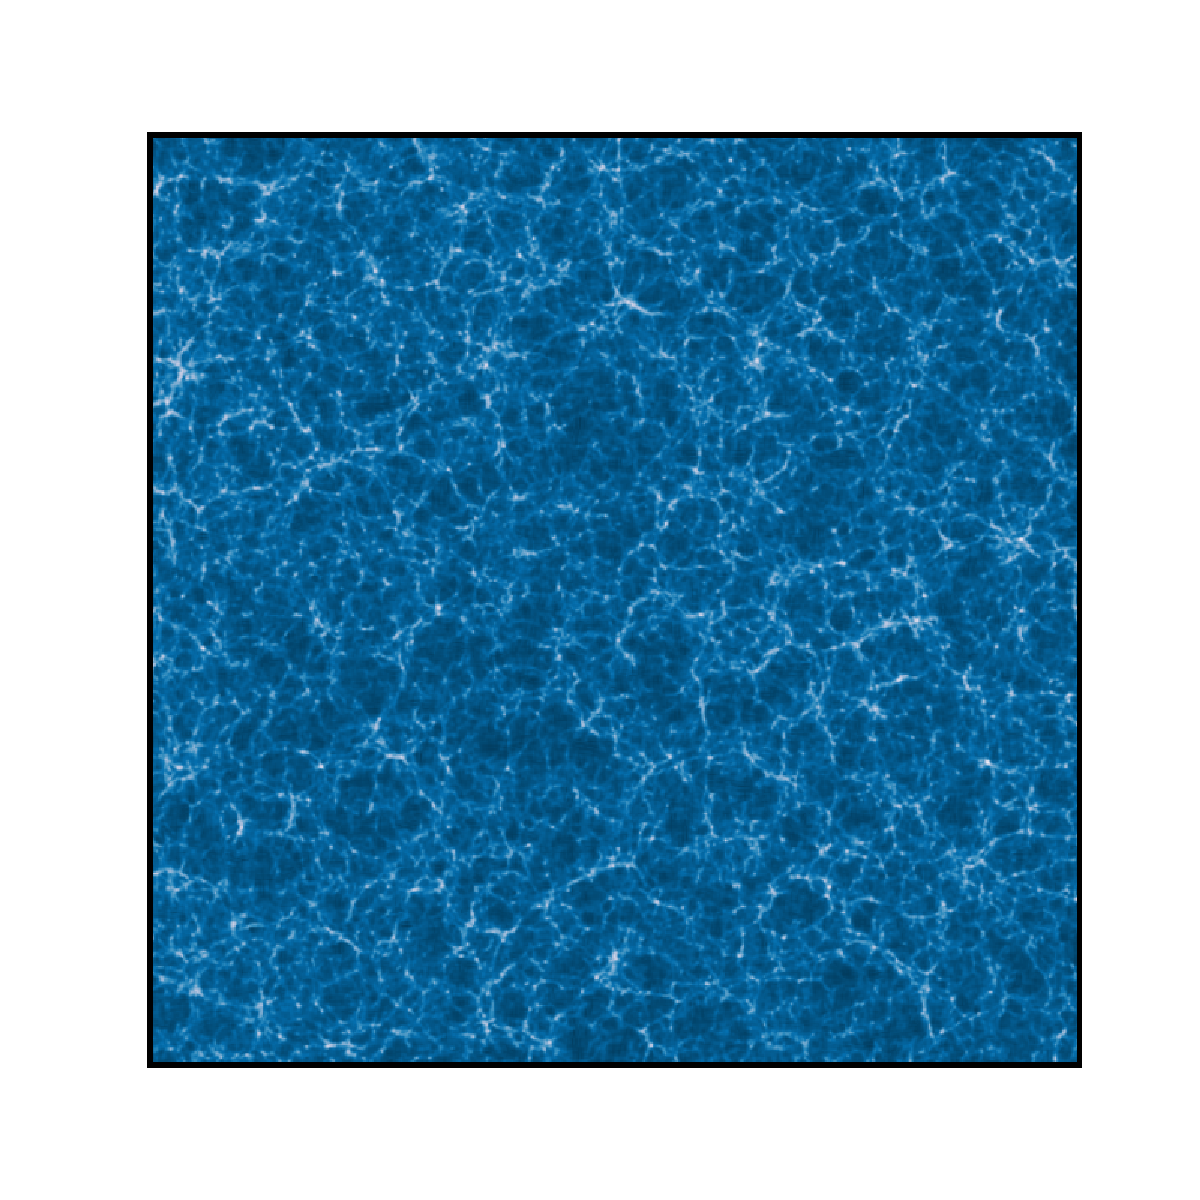
\includegraphics[width=0.3\textwidth]{figures/mocks/fastpm_large.pdf}
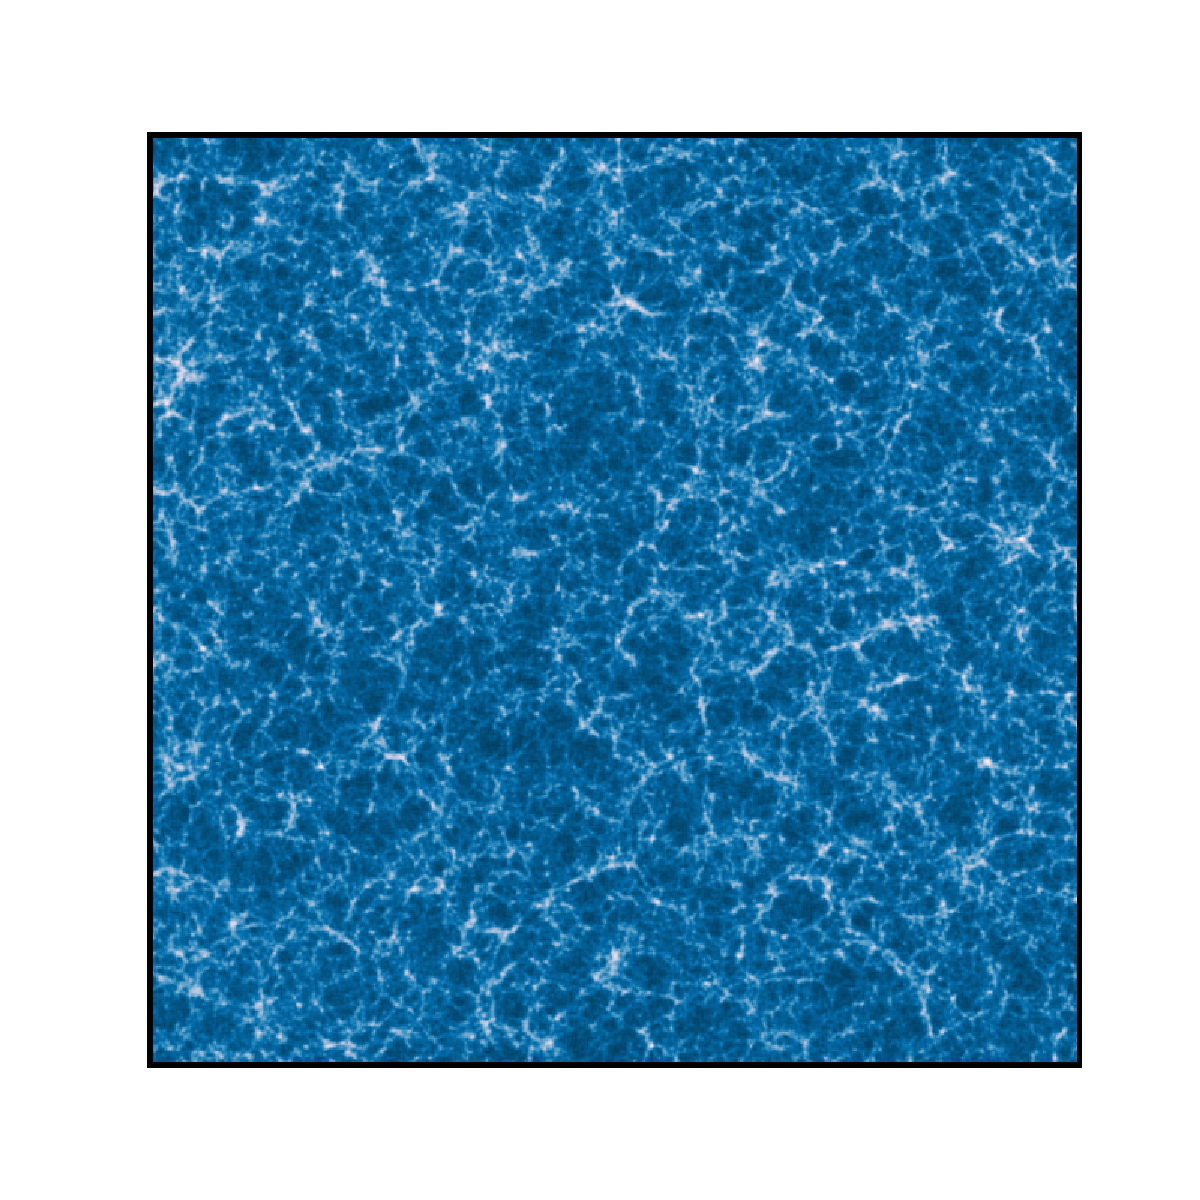
\includegraphics[width=0.3\textwidth]{figures/mocks/alpt_large.pdf}\\
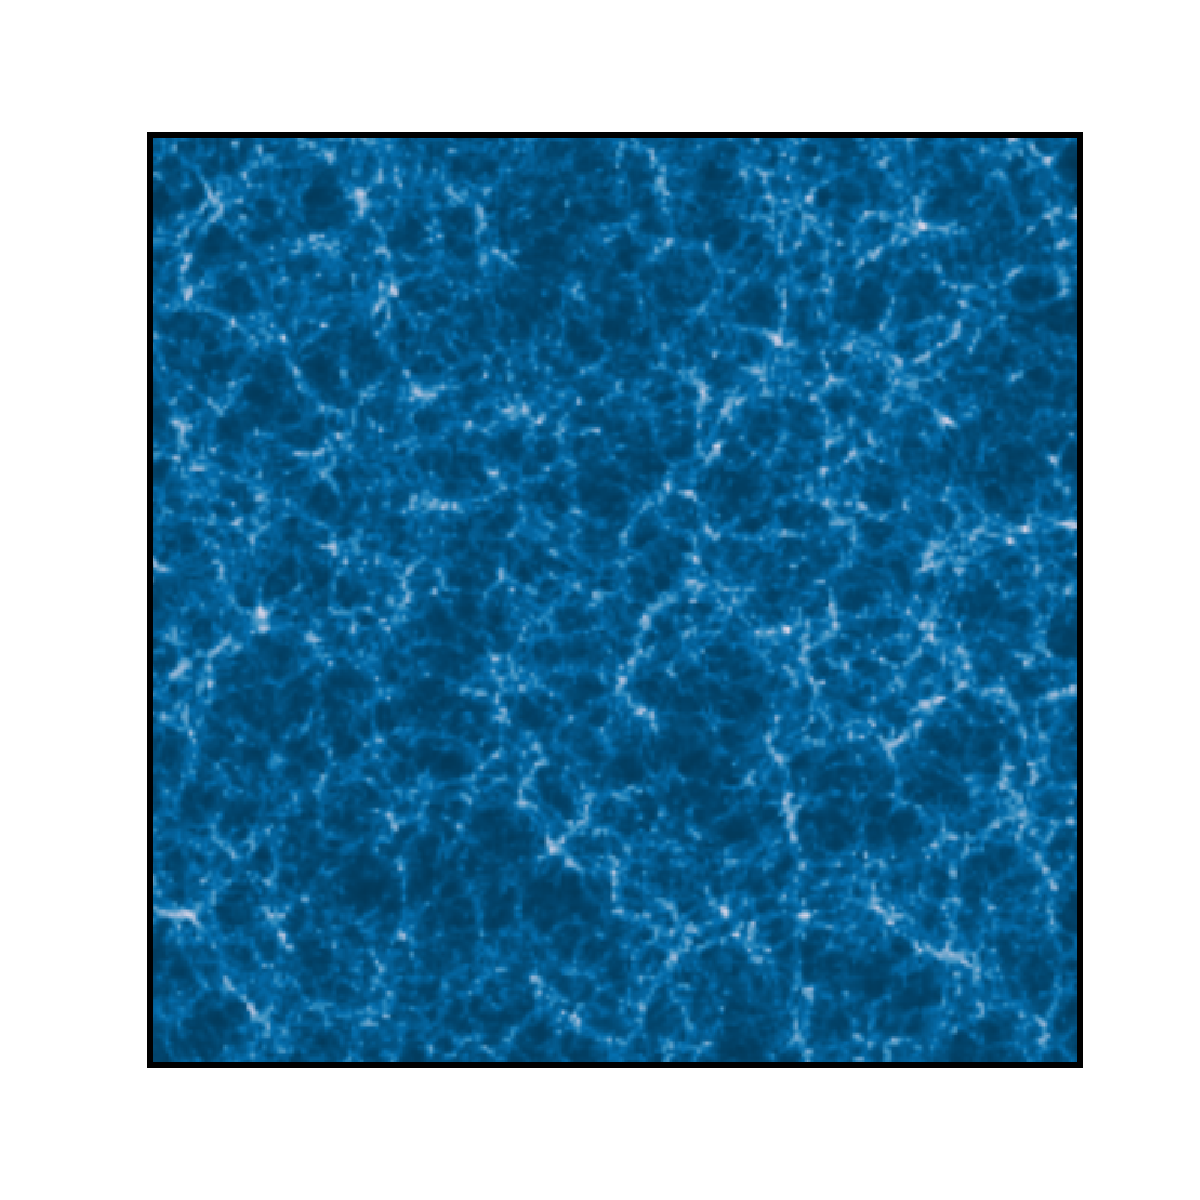
\includegraphics[width=0.3\textwidth]{figures/mocks/bigmd_medium.pdf}
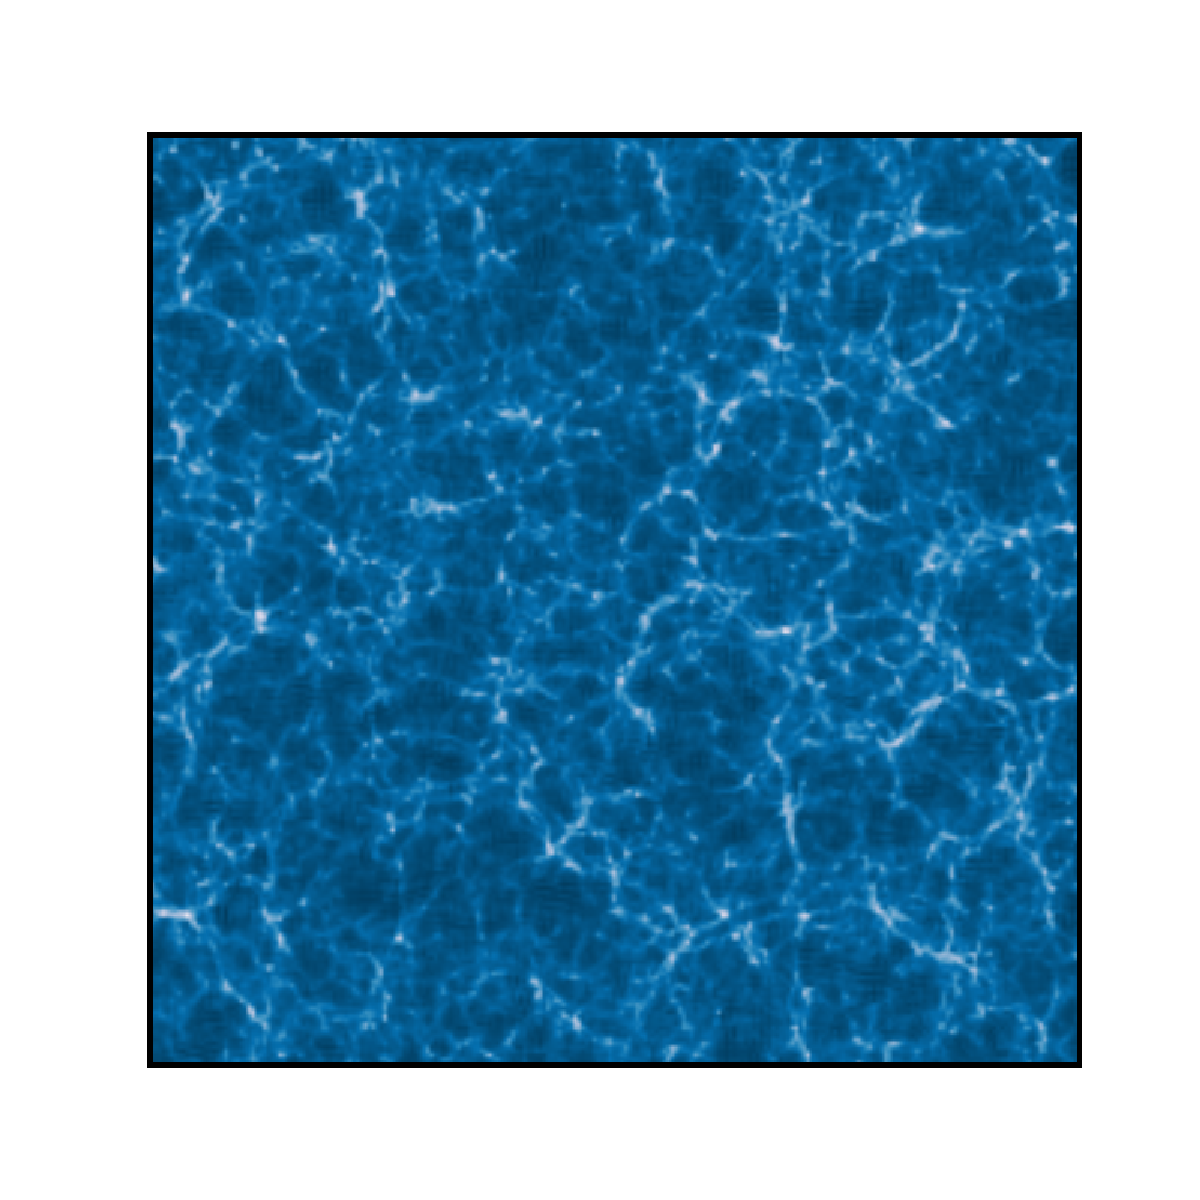
\includegraphics[width=0.3\textwidth]{figures/mocks/fastpm_medium.pdf}
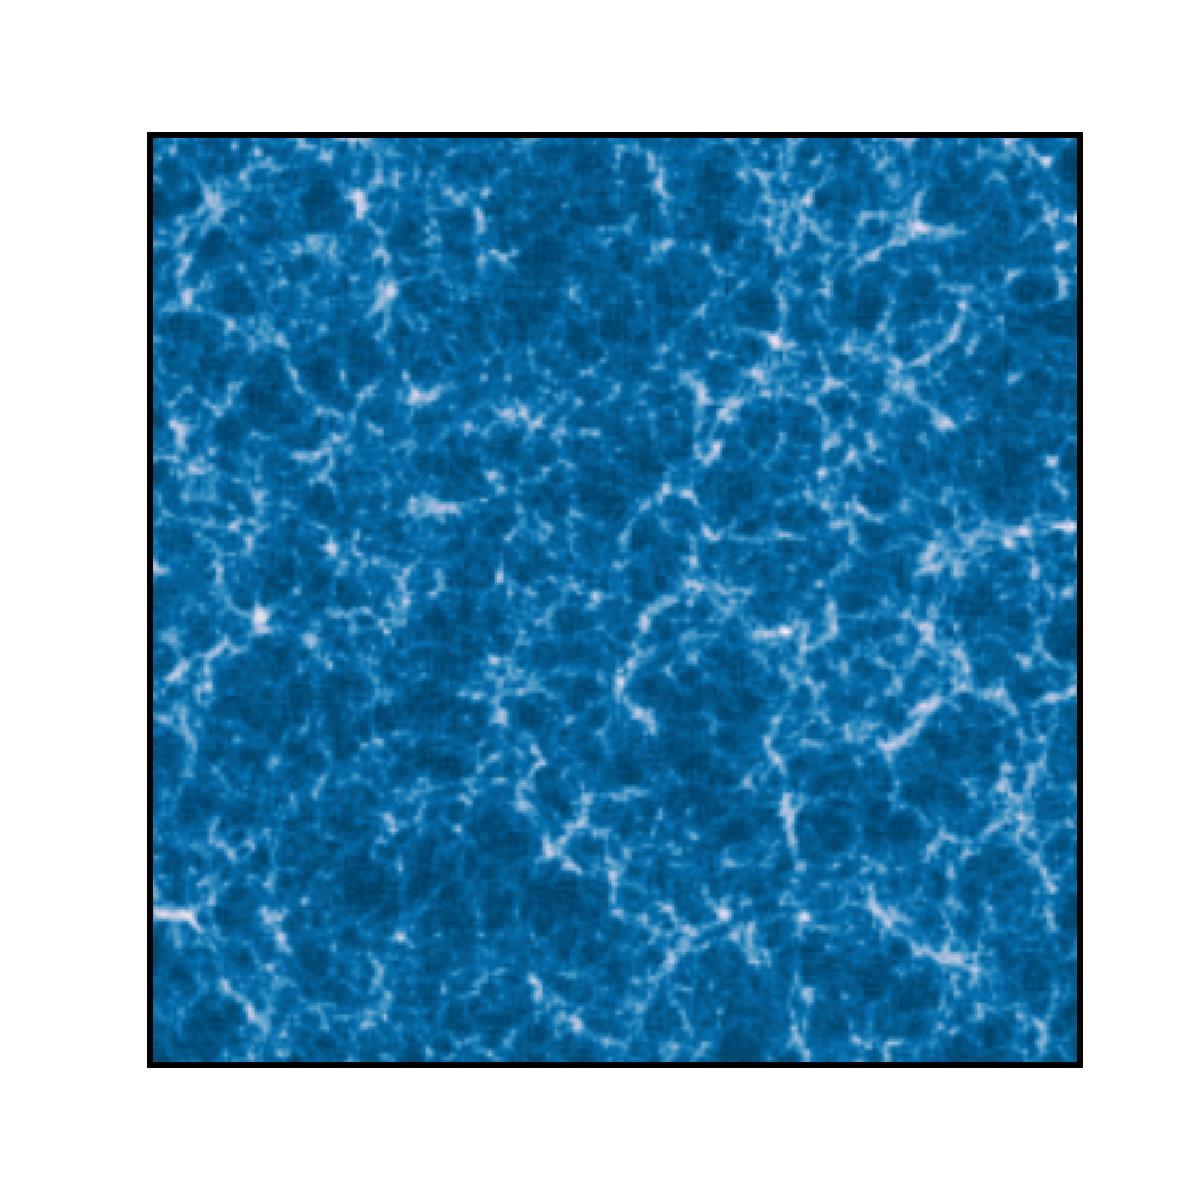
\includegraphics[width=0.3\textwidth]{figures/mocks/alpt_medium.pdf}\\
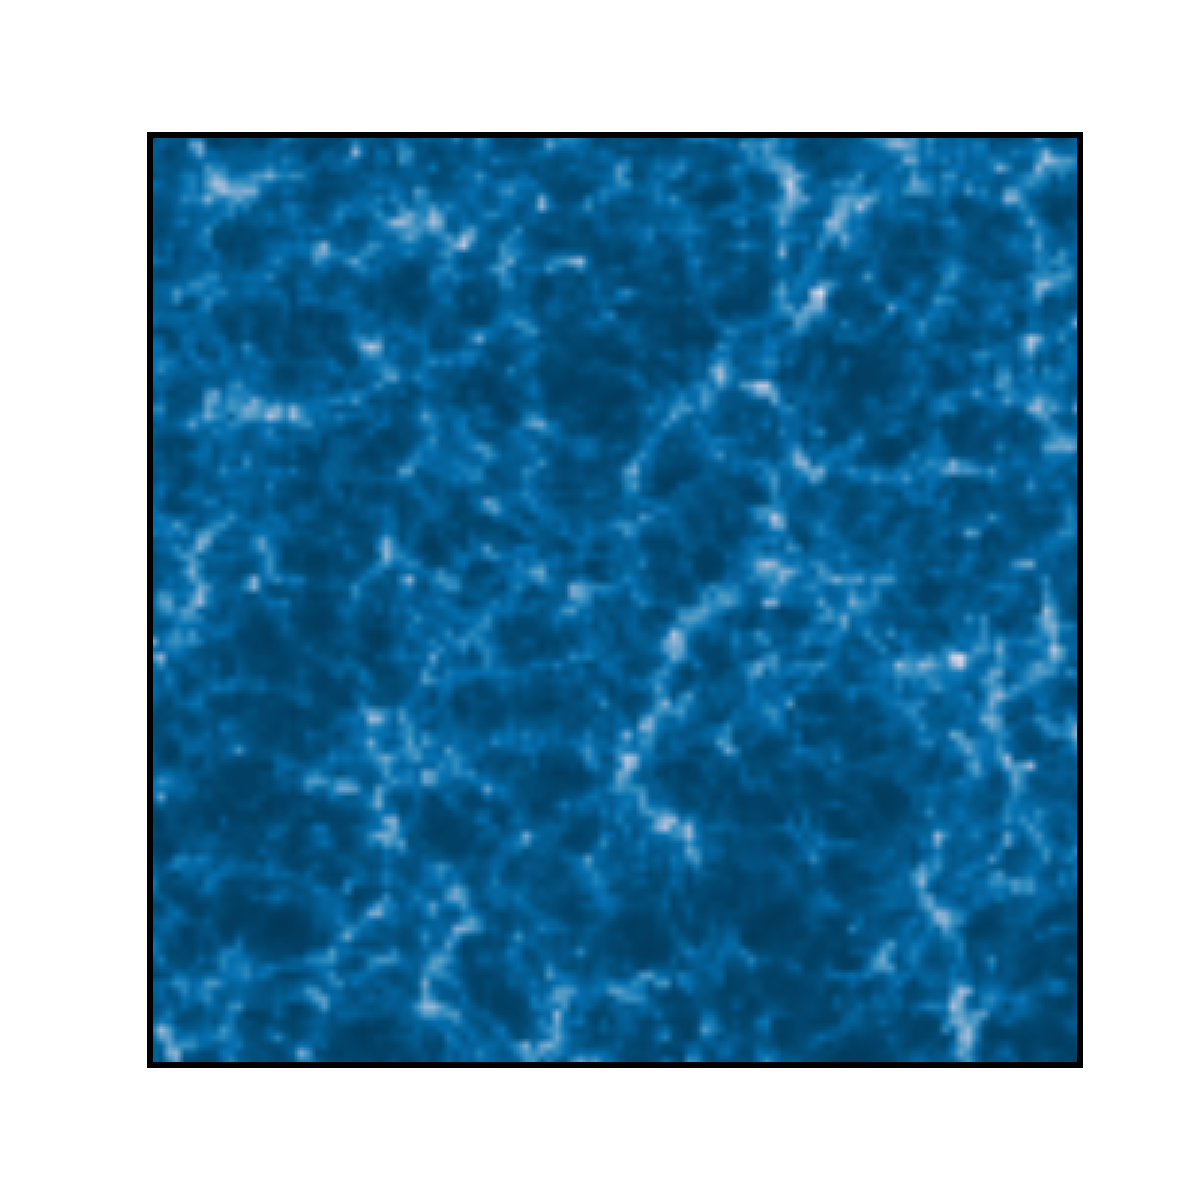
\includegraphics[width=0.3\textwidth]{figures/mocks/bigmd_small.pdf}
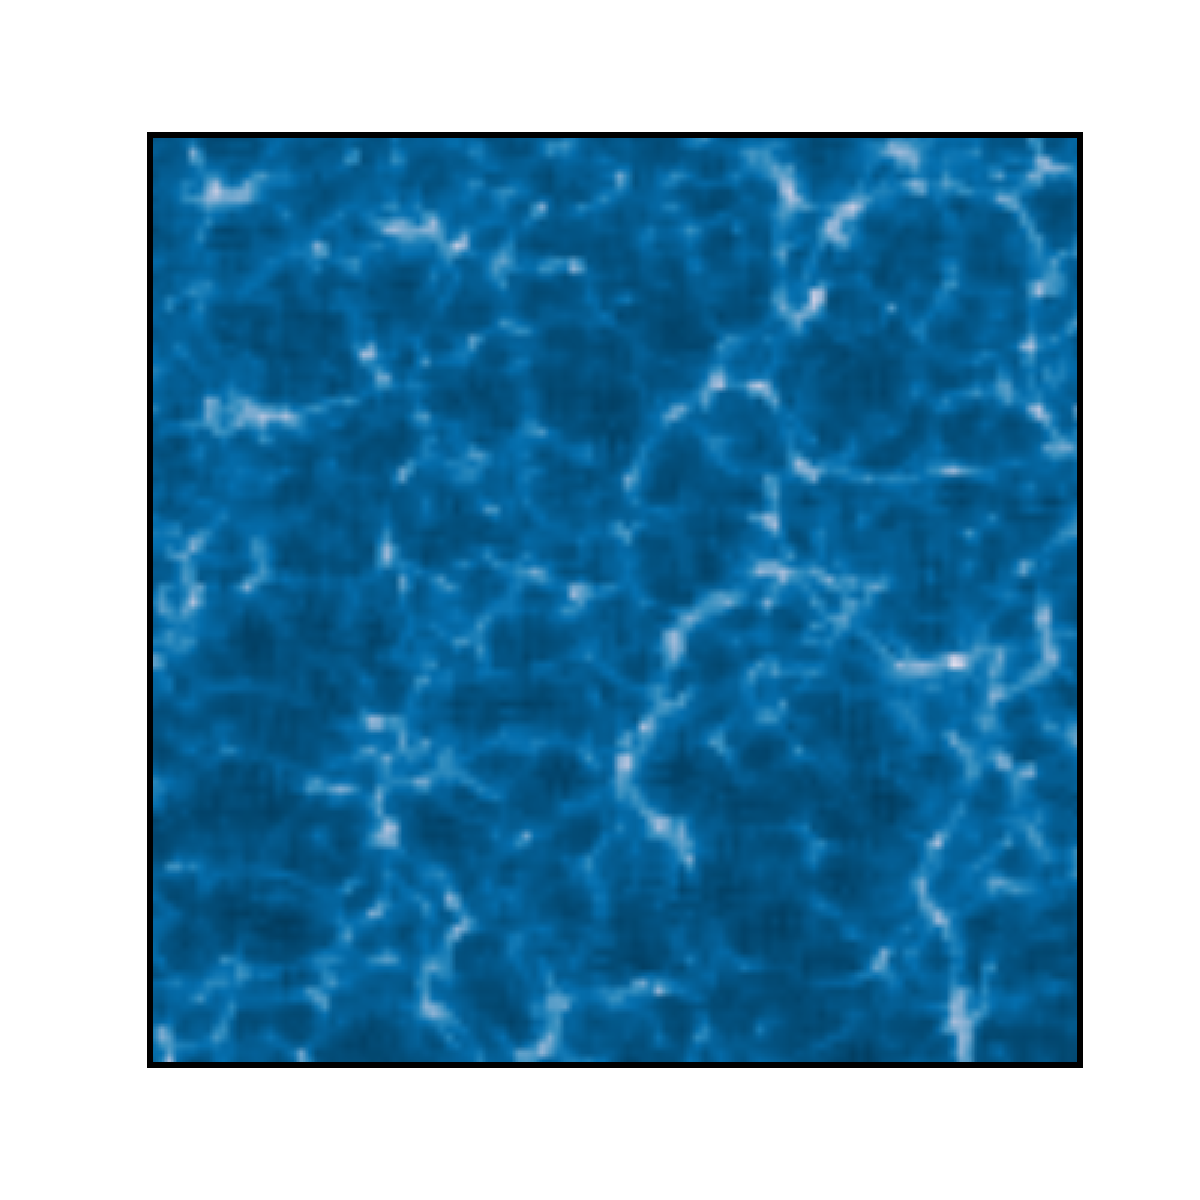
\includegraphics[width=0.3\textwidth]{figures/mocks/fastpm_small.pdf}
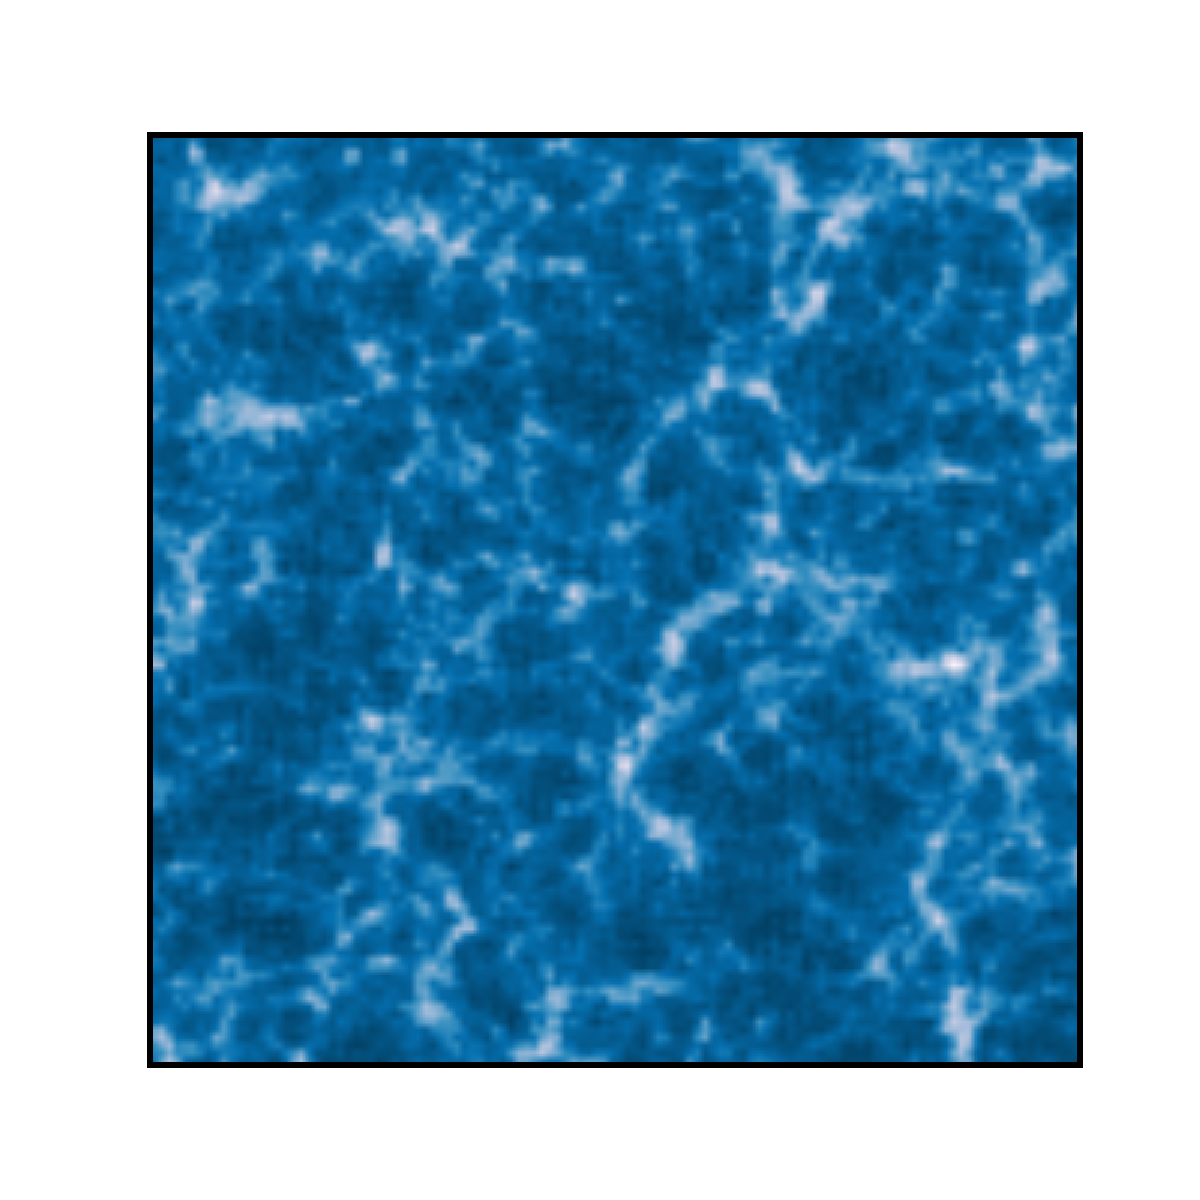
\includegraphics[width=0.3\textwidth]{figures/mocks/alpt_small.pdf}
\end{tabular}
\caption{\label{fig:darkmatter} Dark matter overdensity $\delta = \rho_{\rm m}/\rho -1$ slices of 20 $\mperh$ from the high-resolution BigMultiDark simulation (left panels) , the low-resolution \textsc{FastPM} simulation (central panels) and from the \textsc{alpt} simulation (right panels), taking a subvolume of $(1250 \;\mperh)^3$ (top panels), $(625 \;\mperh)^3$ (middle panels), and $(312.5 \;\mperh)^3$ (bottom panels). The structures in the high-resolution $N$-body simulation and the low-resolution \textsc{FastPM} simulation look very similar inspite of having very different resolutions ($3840^3$ vs $960^3$ particles). The low-resolution \textsc{alpt} simulation looks more diffuse.}
\end{figure*}

\subsection{Structure formation model}
\label{sec:sf}

Originally, the \textsc{patchy} code used Augmented Lagrangian Perturbation Theory (\textsc{alpt}, \citealt{alpt}) as a structure formation model. In this model the second order Lagrangian perturbation theory is modified by employing a spherical collapse model on small comoving scales ($r\leq 2\;\mperh$). 
Any LPT based approximation will lack the one halo term in the clustering. This can be partially compensated within the bias model, however, at the price of obtaining a less accurate description of the biasing relation.
Therefore we introduce in this work within the \textsc{patchy} code the fast particle mesh code \textsc{FastPM} \citep{fastpm}. 
In \textsc{FastPM}, the kick and drift steps of the PM codes are modified such that the linear growth of structure is exact. \citet{fastpm} demonstrate that the memory requirements of this algorithm are much lower than those of the COmoving Lagrangian Acceleration $N$-body solver \citep[\textsc{cola},][]{cola2013}. 

Moreover, \citet{fastpm} shows that running the code with relatively few time steps, and applying a friends-of-friend (hereafter fof) halo finder (\citealt{fof}) to the density field, one can accurately recover the redshift space power spectrum of the fof halos of TreePM accurate $N$-body solver (\citealt{treepm}) down to $k \sim 0.5 \; \hperm$ . The linking length of 0.2 was chosen to be consistent with other works in the literature (\citealt{cola2013}). In this work, we run the \textsc{FastPM} code with 10 time steps. 

In this work we will use as a reference the high-resolution $N$-body BigMultiDark simulation described in more detail in section \S \ref{sec:reference}.
A comparison of the dark matter density fields obtained with the different methods is shown in Fig.~\ref{fig:darkmatter}. While the structures in the high-resolution $N$-body simulation and the low-resolution \textsc{FastPM} simulation look very similar inspite of having very different resolutions ($3840^3$ vs $960^3$ particles), the low-resolution \textsc{alpt} simulation looks more diffuse due to the exaggerated shell crossing inherent to LPT based methods. We will study the impact of this inaccuracy in more detail in section \S \ref{sec:stats}. 

\subsection{Sampling halos from the density field}
\label{sec:bias}

In this section, we describe the statistical bias model of the \textsc{patchy} code.  This model generates halos/galaxies from a given dark matter density field and consists of: deterministic bias, stochastic bias, and an additional step for applying redshift space distortions (RSDs) to the catalogs. We describe the bias steps below and leave RSDs for a later work. 

\subsubsection{Deterministic bias}

The expected number of halos $\langle \rho_{\rm h} \rangle$ in a given volume element ${\rm d}V$ (cosmic cell) can be described in general by a deterministic bias relation $B(\rho_{\rm h}|\rho_{\rm m})$:
\be
\langle \rho_{\rm h} \rangle_{{\rm d}V} = f_{\rm h}\, B(\rho_{\rm h}|\rho_{\rm m})\,,
\ee
where $\rho_{\rm m}$ is the matter density field. The prefactor $f_{\rm h}$ is an overall normalization factor which can be determined by requiring the halo density field to have the number density of the reference sample $n_{\rm h}$, i.e., $n_{\rm h}=\langle\langle \rho_{\rm h}\rangle_{{\rm d}V}\rangle_{V}$. Formally, this can be written as 
\be
f_{\rm h} = \frac{n_{\rm h}}{\langle B(\rho_{\rm h}|\rho_{\rm m}) \rangle_{V}}\,,
\ee
where  $\langle \;.\; \rangle_{V}$ is an ensemble volume average. 
In particular, we will adopt the following compact deterministic bias model:
\ba
B(\rho_{\rm h}|\rho_{\rm m}) &=&  \underbrace{\rho_{\rm  m}^\alpha}_{\mathrm{nonlinear \; bias}} \nonumber \\ 
&\times& \underbrace{\theta\big(\rho_{\rm m} - \rho_{\rm th}\big)}_{\mathrm{threshold \; bias}} \; \times \underbrace{\exp \big(-(\rho_{\rm m}/\rho_{\epsilon})^{\epsilon}\big)}_{\mathrm{exponential \; cutoff}}\,,
\label{eq:deterministic}
\ea
where $\rho_{\rm th}$ is the density threshold which suppresses halo formation in under-dense regions, and $\alpha$ is a nonlinear bias parameter.
The threshold bias (\citealt{kaiser1984,bardeen1986,sheth2001,mo2002}) is modeled by a step function $\theta \big(\rho_{\rm m} - \rho_{\rm th}\big)$ (\citealt{kitaura2014}) and an exponential cutoff $\exp \big(-(\rho/\rho_{\epsilon})^{\epsilon}\big)$ (\citealt{neyrinck2014}). 
Therefore, for this particular bias model we have a normalisation of 
\be
f_{\rm h} = \frac{n_{\rm h}}{\langle \theta(\rho_{\rm m}-\rho_{\rm th})\; \rho_{\rm m}^{\alpha}\; \exp \big(-(\rho_{\rm m}/\rho_{\epsilon})^{\epsilon}\big) \rangle_{V}}\,.
\label{eq:normalization}
\ee

The advantage of this kind of bias model is that it is flexible, it is able to incorporate additional terms, and each of the terms have a physical interpretation.
The power law bias stands for one of the simplest possible nonlinear bias models: a linear Lagrangian bias in a comoving framework, which can be derived from the lognormal approximation \citep[see][]{kitaura2015}, and it resumes in one single bias parameter an infinite Taylor expansion of the dark matter density field \citep{cen1993,fry1993,delatorre}.

The threshold bias and the exponential cut-off describe the fact that halos (or galaxies) can only reside in regions which contain a minimum mass. They also represent the loss of information with respect to the full cosmic density field from selecting only gravitationally collapsed objects.


\subsubsection{Stochastic bias}

The number of halos in each cell is drawn from a Negative Binomial (NB) distribution which can be characterized by the expected number of halos in the cell $\lambda_{\rm h} = \langle \rho_{\rm h} \rangle_{{\rm d}V} \times {\rm d}V$, and a parameter $\beta$ which quantifies the stochasticity (deviation of the distribution from Poissonity) in the halo distribution. According to this model, the probability of having $N_{\rm h}$ objects in a volume element is given by
\ba
P(N_{\rm h}|\lambda_{\rm h}, \beta) &=& \underbrace{\frac{\lambda_{\rm h}^{N_{\rm h}}}{N_{\rm h}!}\, e^{-\lambda_{\rm h}}}_{\mathrm{Poisson\; distribution}} \nonumber \\ 
&\times& \underbrace{\frac{\Gamma(\beta+N_{\rm h})}{\Gamma(\beta)(\beta + \lambda_{\rm h})^{N_{\rm h}}}\times\frac{e^{\lambda_{\rm h}}}{(1+\lambda_{\rm h}/\beta)^{\beta}}}_{\mathrm{Deviation\; from\; Poissonity}}\,.
\label{eq:devpois}
\ea
For $\beta\rightarrow\infty$ we can show that the second raw in the above equation goes to one. Since $\Gamma(\beta)=\frac{\Gamma(\beta+1)}{\beta}=\frac{\Gamma(\beta+N_{\rm h})}{\beta(\beta+1)\cdots(\beta+N_{\rm h}-1)}$, the first factor can be written as $\frac{\Gamma(\beta+N_{\rm h})}{\Gamma(\beta)(\beta + \lambda_{\rm h})^{N_{\rm h}}}=\frac{\beta(\beta+1)\cdots(\beta+N_{\rm h}-1)}{(\beta + \lambda_{\rm h})^{N_{\rm h}}}=\frac{(1+1/\beta)\cdots(1+(N_{\rm h}-1)/\beta)}{(1 + \lambda_{\rm h}/\beta)^{N_{\rm h}}}$. It is now straightforward to see that this goes to one for $\beta\rightarrow\infty$. The same happens for the second factor $\frac{e^{\lambda_{\rm h}}}{(1+\lambda_{\rm h}/\beta)^{\beta}}\rightarrow 1$, since $(1+\lambda_{\rm h}/\beta)^{\beta}\rightarrow e^{\lambda_{\rm h}}$ in that limit.

Given a dark matter density field $\rho_{\rm m}$, the halo density field can be constructed by drawing samples from the expected halo density field $\rho_{\rm h}$ with the Negative-Binomial (hereafter NB) distribution (Eq.~\ref{eq:devpois}). This is inspired by the fact that the excess probability of finding halos in high density regions generates over-dispersion \citep[][]{somerville2001,miranda2002}. This over-dispersion is modeled by a NB distribution (\citealt{kitaura2014,neyrinck2014}). 

The stochastic bias stands for the shot noise from the transition of the continuous dark matter field to the discrete halo (or galaxy) distribution. As predicted by \citet{Peebles1980}, it produces a dispersion larger than Poisson, as long as the two-point correlation function remains positive below the scale of the cell size. This is captured by the negative binomial PDF (Eq.~\ref{eq:devpois}).

\subsection{Constraining the bias model}
\label{sec:mcmc}

Production of approximate mock catalogs with \textsc{patchy} requires a reference catalog constructed from the observations or based on an accurate $N$-body simulation. 
We aim at constraining the parameters describing the deterministic bias $\{\delta_{\rm th},\alpha, \rho_{\epsilon},\epsilon\}$, and the parameter that governs the stochasticity of the halo population $\{\beta\}$.

The bias parameters are estimated such that the statistical summaries of the halos (galaxies) in the \textsc{patchy} mocks match the statistical summaries of the halos (galaxies) in the reference catalog. The set of statistical summaries of the catalog can in principle include number density, bivariate probability distribution function or number of counts-in-cells $\rho$ (hereafter halo PDF), two-point statistics $\xi_{2}$, and higher-order statistics such as the three-point statistics $\xi_{3}$. 

By construction, the \textsc{patchy} mocks reproduce the exact number density of objects in the reference catalog. This comes from the particular choice of normalization in the deterministic bias relation (see Eqs.~\ref{eq:deterministic},\ref{eq:normalization}). In this work, we follow \citet{kitaura2015} and constrain the bias parameters with the halo PDF and the two-point statistics $\xi_{2}$. These two quantities can be computed very fast and the skewness of the halo PDF determines the three point statistics. Given the bias parameters found fitting the PDF and the two-point statistics, we will demonstrate a comparison between the approximate mocks and the reference catalog in terms of the two- and three-point statistics. 

We simultaneously fit the real-space power spectrum $P(k)$ and the PDF $\rho(n)$ of the \textsc{patchy} halo density field to $P(k)$ and $\rho(n)$ measured for the BigMuliDark halo catalog. Specifically, constraints on $\theta = \{\delta_{\rm th},\alpha, \rho_{\epsilon},\epsilon, \beta\}$ are found by sampling from the posterior probability $p(\theta|\mathrm{data}) \propto p(\mathrm{ref}|\theta)p(\theta)$, where $\mathrm{ref}$ denotes the combination $\{P_{\rm ref} (k), \rho_{\rm ref}(n)\}$, and the likelihood $p(\mathrm{ref}|\theta)$ is given by
\ba
-2\ln p(\mathrm{ref}|\theta) &=& \Sigma_{k}\frac{\big(P_{\rm ref}(k)-P_{\rm mock}(k)\big)^{2}}{\sigma^{2}_{k}} \nonumber \\
&+& \Sigma_{n}\frac{\big(\rho_{\rm ref}(n)-\rho_{\rm mock}(n)\big)^{2}}{\sigma^{2}_{n}}.
\label{eq:like}
\ea
For the purpose of estimating the bias parameters, we find it sufficient to assume simple uncorrelated noise terms $\{\sigma_{k},\sigma_{n}\}$ in the above likelihood (\ref{eq:like}). We assume $\sigma_{k}^{2}$ to be $4\pi^{2} P_{\rm ref}^{2}(k)/(V_{\rm box}k^{2}\Delta k)$, and $\sigma_n^{2}$ to be $N_n$ where $N_n$ is the number of cells containing $n$ number of halos (including parent halos and subhalos). Furthermore, we choose a flat prior for all parameters of the bias model with the following lower and upper bounds: $-1<\delta_{\rm th}<2$, $0<\alpha<1$, $0<\beta<1$, $0<\rho_{\epsilon}<1$, and $0<\epsilon<1$.

For sampling from the posterior probability, given the likelihood function (Eq.~\ref{eq:like}) and the prior, we use the affine-invariant ensemble MCMC sampler (\citealt{goodmanweare}) and its implementation \textsc{emcee} (\citealt{emcee}). In particular, we run the \textsc{emcee} code with 10 walkers and we run the chains for at least 2000 iterations. We discard the first 500 chains as burn-in samples and use the remainder of the chains as production MCMC chains. Furthermore, we perform Gelman-Rubin convergence test (\citealt{grtest}) to ensure that the MCMC chains have reached convergence.

\subsection{Comparison with other approximate methods}

Pioneering fast halo/galaxy generating methods have relied on approximate gravity solvers based on Lagrangian perturbation theory (LPT) to compute the position and mass of the objects, such as \textsc{Pinocchio} (Zeldovich: \citealt{monaco2002,monaco2013}, 3LPT: \citealt{monaco2016}) and \textsc{PThalos} (2LPT: \citealt{buchert1993,bouchet1995,catelan1995,scocci2002,pthalo,manera2015}).
This has the disadvantage of being affected by an inaccurate description of the small scale clustering, and, in particular, of missing the one halo term contribution. As a consequence, the power spectra of such catalogs have systematic deviations towards high values of $k$, already deviating about 10$\%$ at $k\sim0.2\; \hperm$ \citep[][]{monaco2013}.

While fast particle mesh solvers, such as \textsc{cola} or \textsc{FastPM}, are much more precise than LPT based approaches, they are  still computationally too expensive to be suitable for massive production, if one is trying to resolve all the necessary structures required to interpret the next generation of galaxy surveys.
Therefore three methods were recently proposed: \textsc{patchy} \citep{kitaura2014}, \textsc{QPM} \citep{qpm}, and \textsc{EZmocks} \citep{eazymock}, which do not try to resolve halos (nor galaxies) with the approximate gravity solvers, but just get a reliable large scale dark matter field, which can then be populated with some bias prescription. The gravity solver thus only needs to be accurate on a certain scale, then the halo/galaxy-dark matter connection is exploited to reach a high accuracy, as described above.
These methods use both different gravity solvers and different bias models. While \textsc{patchy} originally relies on \textsc{alpt}, \textsc{QPM} uses a quick particle mesh solver, and \textsc{EZmocks} uses the Zeldovich linear LPT.
But more importantly the bias prescription follows very different philosophies. \textsc{QPM} uses a rank ordering scheme relating the halo mass to density peaks. However, a recent study  demonstrated  that the dependence of the halo mass to its environment is not trivial \citep[see][]{zhao2015}.  \textsc{EZmocks}, on the other hand, first modifies the initial power spectrum introducing a tilt to adjust the final two point statistics, correcting hereby the missing one halo term of the approximate gravity solver. Second it imposes the halo PDF, which was shown to determine the 3pt statistics \citep{kitaura2015}.
\textsc{patchy} on the other hand follows a more physical approach, relying on an effective analytical stochastic bias model. 
In this sense the statistics is not directly imposed as in \textsc{EZmocks}, but fitted through the bias parameters. In fact \textsc{patchy} was shown to be considerably more accurate than \textsc{EZmocks} when assigning halo masses \citep{zhao2015}, and than \textsc{QPM} when fitting the two and three point statistics of the luminous red galaxies (LRGs) in the Baryon Oscillation Spectroscopic Survey (BOSS)  \citep{kitaura2016}. 

Moreover, the approach we follow in \textsc{patchy} tests the validity range of effective bias prescriptions commonly used in large scale structure analysis methods \citep[see e.g.][]{ata2015}.

Now for the first time we include a robust MCMC sampling scheme to determine the bias parameters, and have improved the gravity solver with \textsc{FastPM}.

\begin{figure*}
%\begin{center}
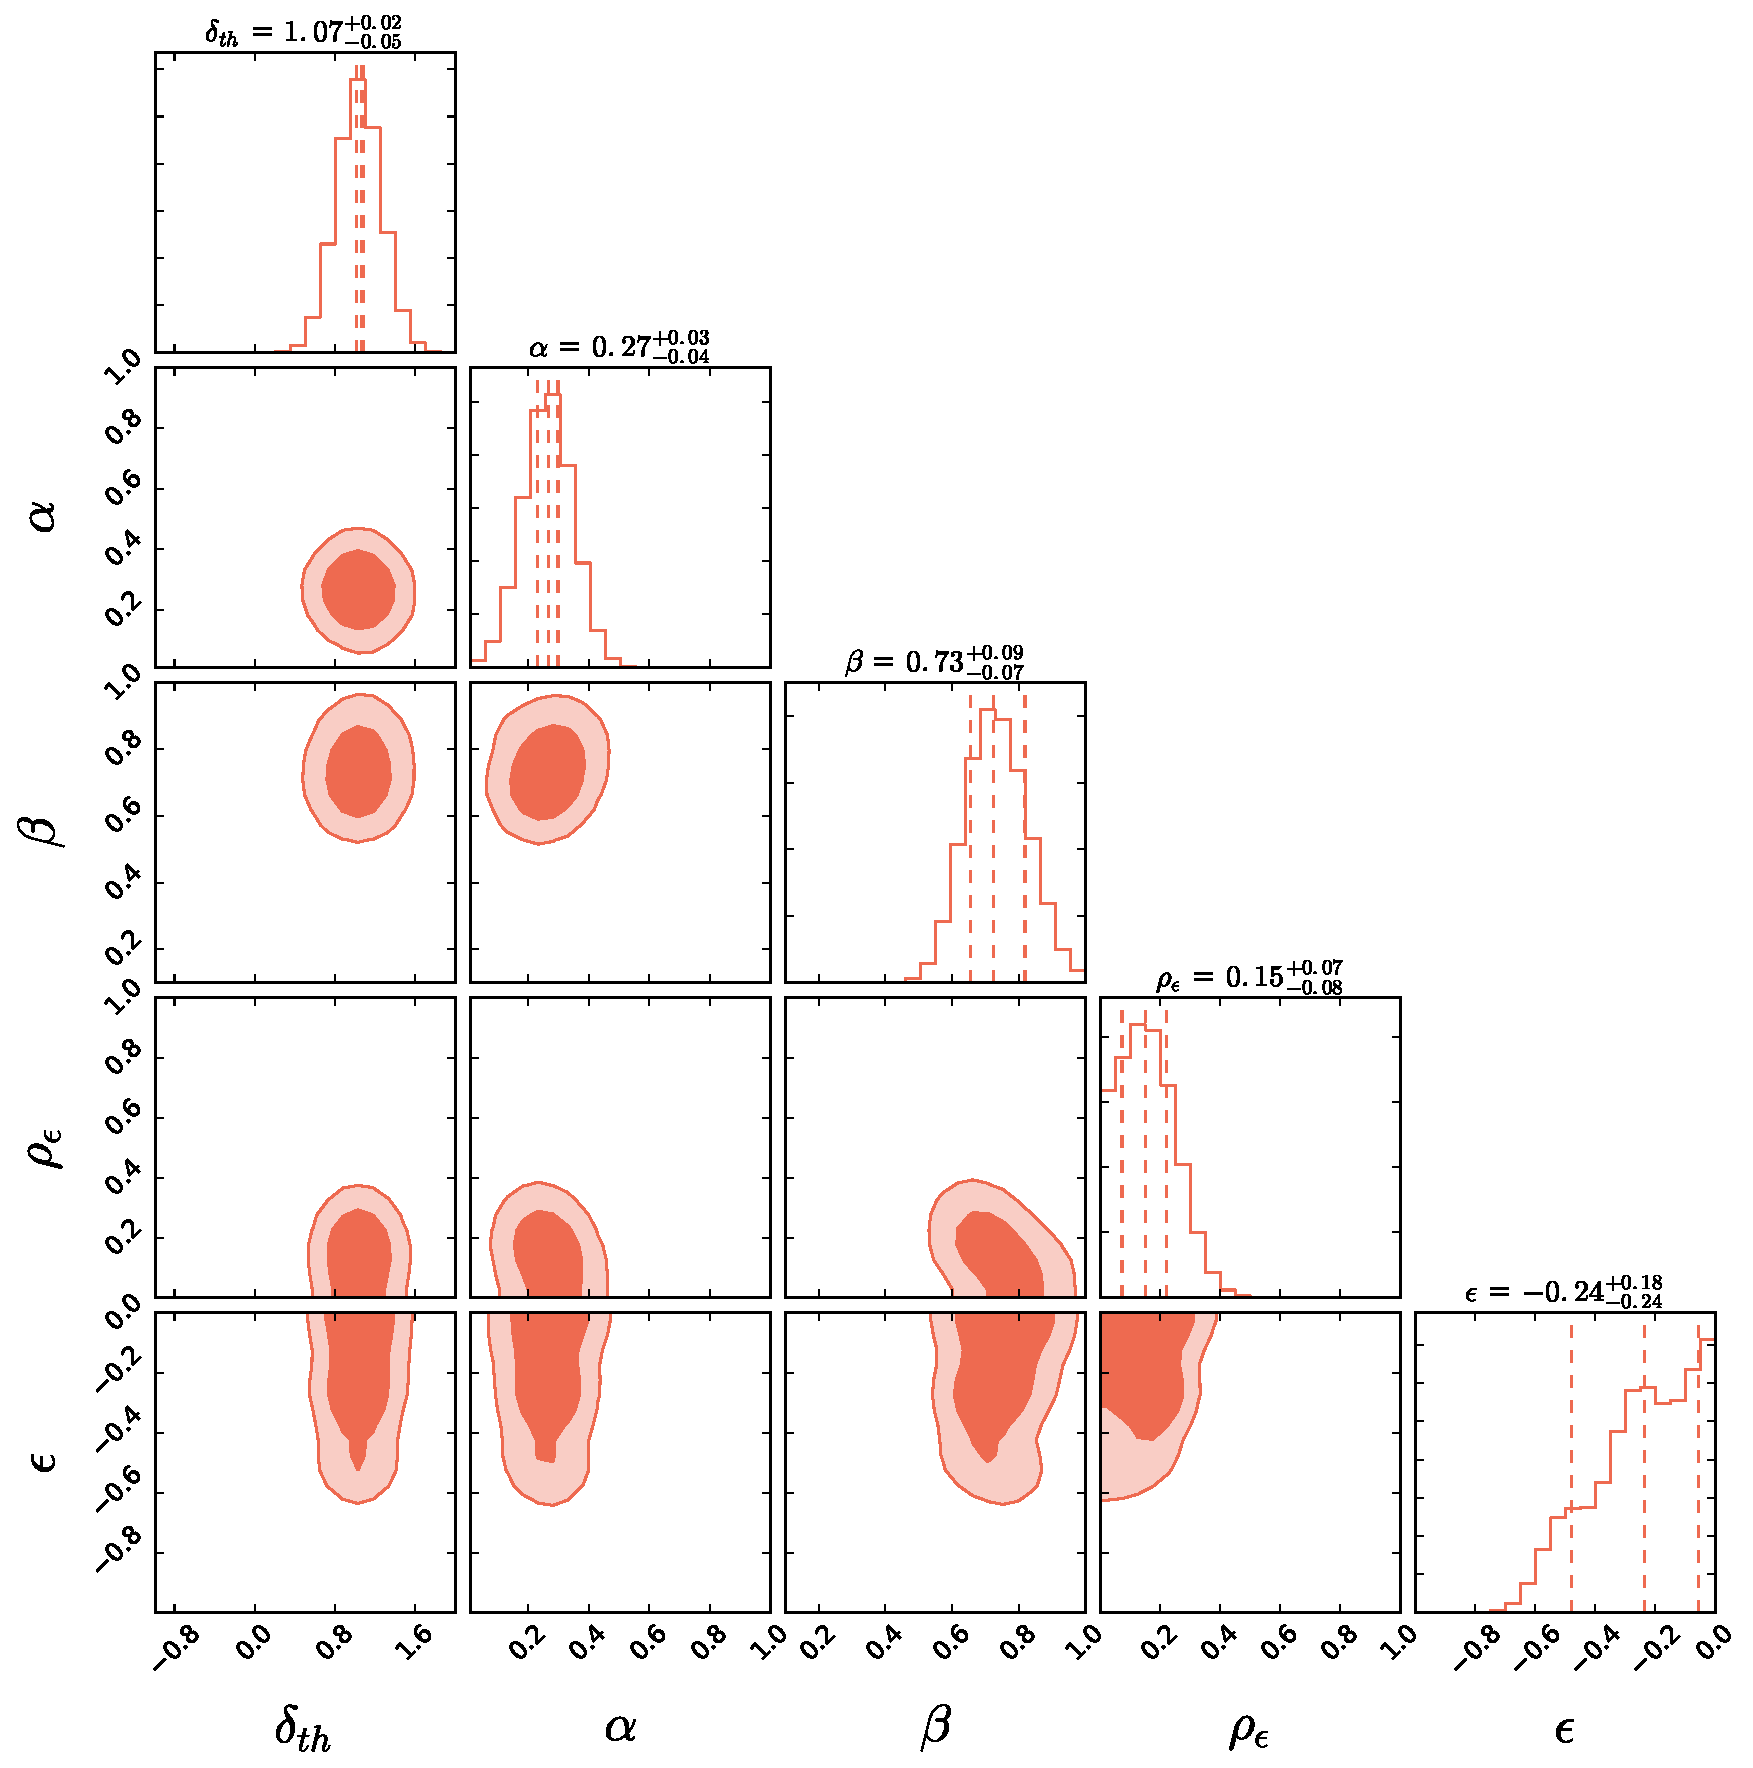
\includegraphics[width=0.9\textwidth]{figures/mocks/posterior.pdf}
\caption{\label{fig:bias2} Posterior probability distribution of the \textsc{patchy} bias parameters $\{\delta_{\rm th},\alpha,\beta,\rho_{\epsilon},\epsilon\}$. The contours mark the 68$\%$ and the 95$\%$ confidence intervals of the posterior probabilities. This plot is made using the open-source software \textsc{corner} (\citealt{corner}).}
%\end{center}
\end{figure*}

\begin{figure*}
 \begin{tabular}{cc}
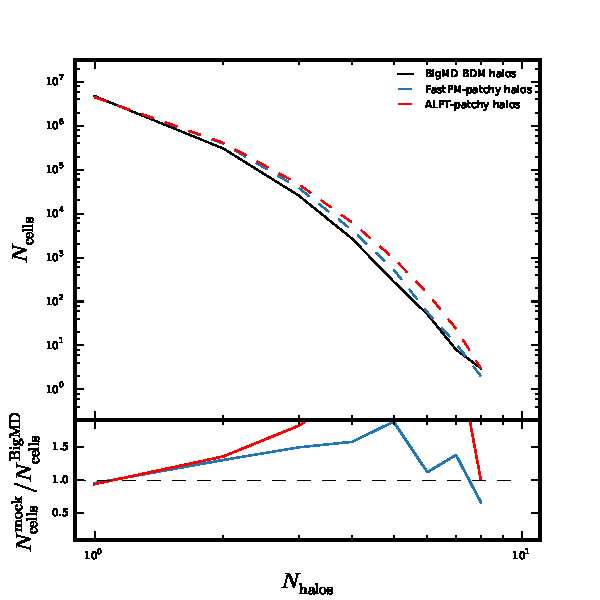
\includegraphics[width=0.4\textwidth]{figures/mocks/pdf.pdf}
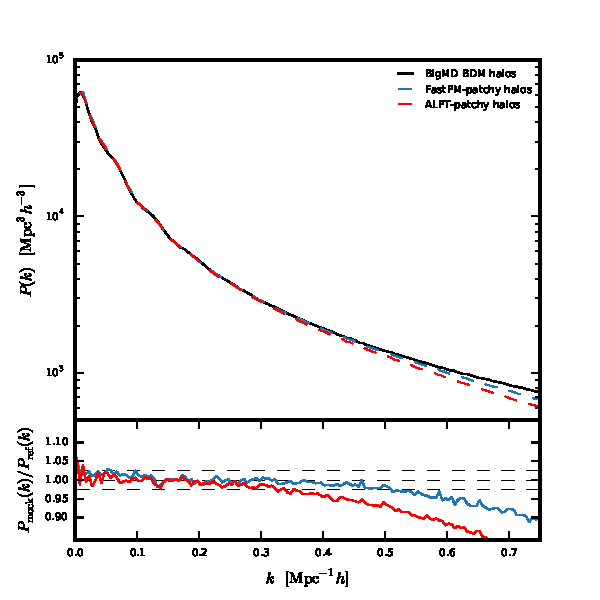
\includegraphics[width=0.4\textwidth]{figures/mocks/pk.pdf}
\end{tabular}
\caption{\label{fig:pdfpower} Top: Demonstration of the halo bivariate probability distribution function of halos (halo counts-in-cells) in the BigMultiDark simulation (shown in black) and in the \textsc{FastPM}-\textsc{patchy} simulation (shown in blue) and in the \textsc{alpt}-\textsc{patchy} simulation (shown in red) on the left. Comparison between the real-space power spectrum of the BDM halos (shown in black) in the reference BigMultiDark simulation and that of the halos in the \textsc{FastPM}-\textsc{patchy} (\textsc{alpt}-\textsc{patchy}) simulation shown in blue (red) on the right. 
Bottom: Ratio between the halo PDFs of the approximate mocks and halo PDF of the BigMultiDark simulation on the left. Ratio between the halo power spectra of the approximate mocks and the halo power spectrum of the BigMultiDark simulation on the right.}
\end{figure*}

\begin{figure*}
\vspace{-0.5cm}
\begin{tabular}{cc}
%\hspace{-0.4cm}
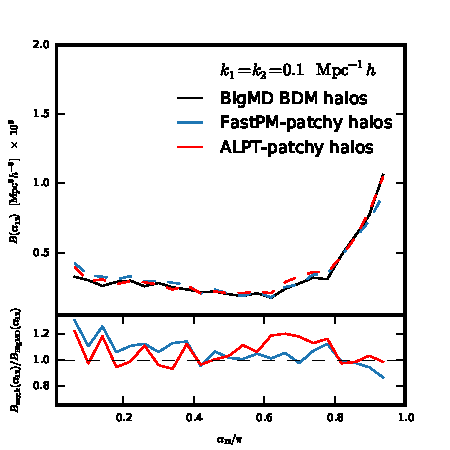
\includegraphics[width=0.4\textwidth]{figures/mocks/bispec1.pdf}
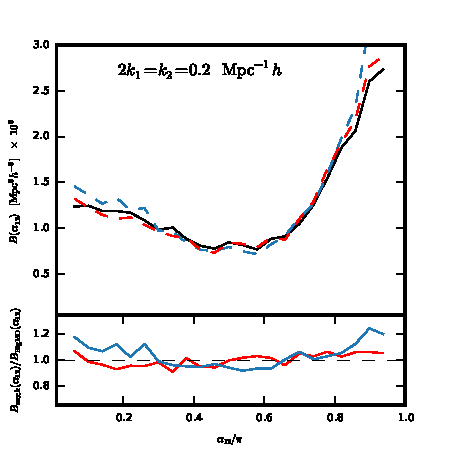
\includegraphics[width=0.4\textwidth]{figures/mocks/bispec3.pdf}
\vspace{-0.8cm}
\\
%\hspace{-0.4cm}
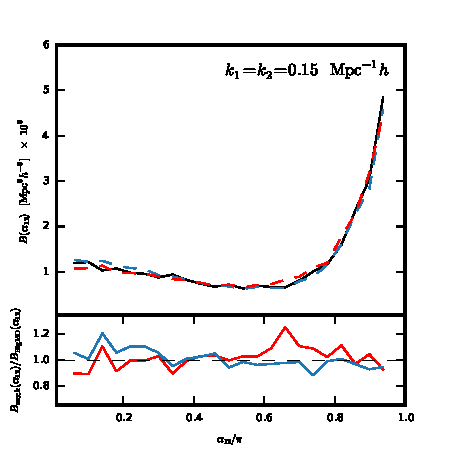
\includegraphics[width=0.4\textwidth]{figures/mocks/bispec2.pdf}
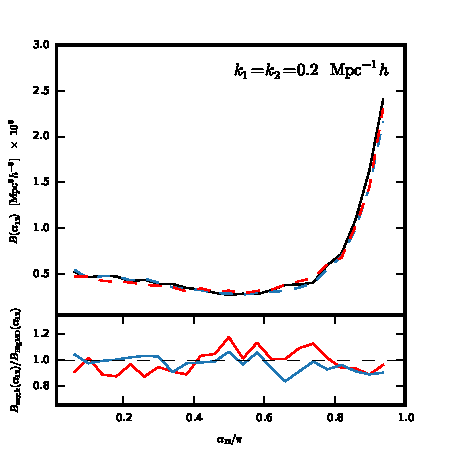
\includegraphics[width=0.4\textwidth]{figures/mocks/bispec5.pdf}
\vspace{-0.8cm}
\\
%\hspace{-0.4cm}
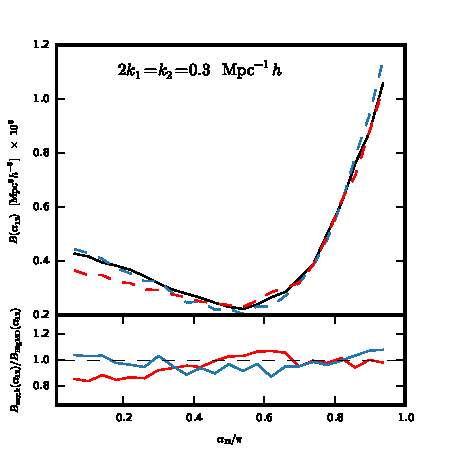
\includegraphics[width=0.4\textwidth]{figures/mocks/bispec4.pdf}
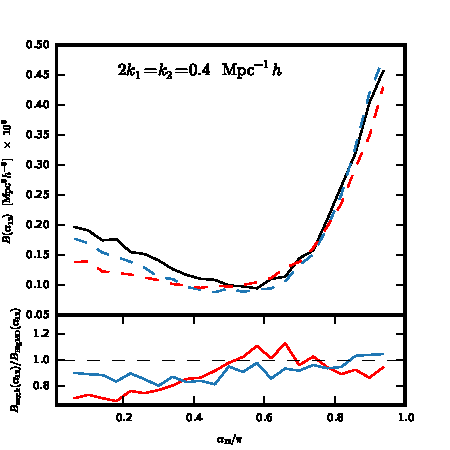
\includegraphics[width=0.4\textwidth]{figures/mocks/bispec6.pdf}
\vspace{-0.25cm}
\end{tabular}
\caption{\label{fig:bispec} Real-space bispectrum of the BigMD BDM halos and that of the approximate mocks as a function of angle $\alpha_{12}$ between $\mathbf{k}_1$ and $\mathbf{k}_{2}$ for $k_{1}=k_{2}=0.1\; \hperm$ (upper left), $2k_{1}=k_{2}=0.2\; \hperm$ (upper right), $k_{1}=k_{2}=0.15\; \hperm$ (middle left), $k_{1}=k_{2}=0.2\; \hperm$ (middle right), $2k_{1}=k_{2}=0.3\; \hperm$ (lower left), and $2k_{1}=k_{2}=0.4\; \hperm$ (lower right). The BigMD is represent by the solid black line, while \textsc{alpt}-\textsc{patchy} is represented by the dashed red line, and \textsc{FastPM}-\textsc{patchy} is represented by the dashed blue line.}
\end{figure*}


\section{Demonstration on an accurate $N$-body based halo catalog}
\label{sec:mocktest}

In this section we present the application of the above described method to a well studied case: the halo distribution required to describe the CMASS LRG sample of the BOSS survey \citep{white2011,Dawson2013}.
First, we briefly describe the reference catalog and then present a detailed statistical analysis of the results.

\subsection{Reference catalog}
\label{sec:reference}

For the reference simulation used in this work we rely on the Bound-Density-Maxima (BMD, \citealt{bdm}) halo catalogs in the $z=0.5618$ snapshot of the BigMultiDark-Planck high 
resolution $N$-body simulation \citep{multidark}. This simulation was carried out using the L-Gadget2 code \citep{gadget}, following the Planck $\Lambda$CDM cosmological parameters 
$\Omega_{\rm m} = 0.307$, $\Omega_{\rm b} = 0.048$, $\Omega_{\Lambda} = 0.693$, $\sigma_{8} = 0.823$, $n_{\rm s}=0.96$, 
$h=0.678$. The box size for this $N$-body simulation is 2500 $\mperh$, the number of simulation particles is 3840$^3$, 
the mass per simulation particle $m_{\rm p}$ is $2.359 \times 10^{10} \; h^{-1} M_{\odot}$, and the gravitational softening length 
$\epsilon$ is 30 $h^{-1} \rm{kpc}$ at high-$z$ and 10 $h^{-1} \rm{kpc}$ at low-$z$.

A minimum mass cut of $0.5 \times 10^{13} \; h^{-1} M_{\odot}$ has been applied to the halo catalog so that it matches with the number density of the SDSS III-BOSS CMASS galaxy catalog \citep{white2011,Dawson2013}. After applying the mass cut, the number density of the final catalog is 3.5 $\times 10^{-4}$ $(\hperm)^{3}$. The MultiDark-\textsc{patchy} galaxy catalogs \citep{kitaura2016} are calibrated against BOSS-HAM catalogs which were constructed by populating the halos in different snapshots of the BigMultiDark simulation using halo abundance matching \citep{sergio2016}.   

Evaluation of $P(k)$ and $\rho(n)$ for a set of bias parameters requires running the forward model of generating halos from the matter density field. Therefore, in order to speed up the fitting procedure we run the \textsc{patchy} code with a smaller box size of 625 $\mperh$ and grid size of 240 in each dimension. This choice of box and grid size preserves the resolution. Furthermore, running the \textsc{patchy} code and computing the statistics of the halo catalogs in a smaller box size significantly reduces the computational time needed for constraining the bias parameters.

\subsection{Bias parameters}

The first step in our pipeline consists of producing the large scale dark matter field on a mesh. We use the down-sampled  white noise of the BigMultiDark simulation from $3840^3$ to $960^3$ cells to estimate the initial conditions used for both \textsc{FastPM} and \textsc{alpt} runs, as shown in Fig.~\ref{fig:darkmatter}. The dark matter particles are then assigned to a mesh of $960^3$ cells with clouds-in-cells (CIC), which we define as the large scale dark matter density field $\rho_{\rm m}$ required for Eqs.~\ref{eq:deterministic}, \ref{eq:normalization}, \ref{eq:devpois}. 

After running the MCMC chains with the method described in section \S \ref{sec:mockmethod}, we find constraints on the bias parameters of such equations. These constraints are summarized in Fig.~\ref{fig:bias2}.  
The threshold bias parameter $\delta_{\rm th}$ is found to be 1.07 which is equivalent to sampling halos from the regions of high matter overdensity. This supports our intuition that massive halos are generated from high density regions. Our estimated value of the nonlinear bias parameter $\alpha$ is $\sim$ 0.2. These values are qualitatively consistent with \textsc{alpt} \citep{kitaura2014}, although the threshold bias is slightly reduced and the power law bias is slightly higher (parameters with \textsc{alpt}: $\delta_{\rm th} \sim 1.2$ and $\alpha \sim 0.12$).

The parameter that governs the deviation from Poissonity $\beta$ is found to be $~ 0.73$. This value is significantly larger than the one found with \textsc{alpt} (about 0.6), i.e., indicating that the deviation from Poissonity is not so pronounced as previously found. The reason for this, is that Lagrangian perturbation theory does not manage to model the one halo term, as done with \textsc{FastPM}. Therefore a larger deviation of Poissonity had to be assumed to fit the power spectrum towards small scales, as is demonstrated here. In this sense, a more accurate description of the large scale dark matter field permits us to reduce the stochasticity in the halo distribution.

Furthermore, parameters corresponding to the exponential cutoff term in the deterministic bias relation $\{\rho_{\epsilon},\epsilon\}$ are estimated to be $\sim \{0.15,-0.24\}$. While the constraints on both parameters of the exponential cutoff bias are consistent with zero, their presence, albeit being small, is essential in a more accurate modeling of the halo bivariate PDF and the halo bispectrum. By including these extra parameters we demonstrate the flexibility and  efficiency of the code to incorporate complex bias models. Furthermore, we believe that the  exponential cutoff term will become crucial when considering smaller mass halos, which have a non negligible probability of residing in low density regions \citep[][]{neyrinck2014}.


\subsection{Statistical comparison}
\label{sec:stats}

In this section we discuss the statistical comparisons between the BDM halo catalog of the BigMultiDark simulation and the halo catalog generated from our method. In particular, the \textsc{FastPM}-\textsc{pathcy} mock is generated using the best-fit bias parameters (see Fig.~\ref{fig:bias2}). For the \textsc{alpt}-\textsc{pathcy} mocks we rely on the parameters found from previous \textsc{patchy} studies \citep{kitaura2016}. The halo statistical summaries presented in this work are the number density, the bivariate halo probability distribution function (PDF), the real-space power spectrum and the real-space bispectrum. 

By construction our method reproduces the exact number density of halos in the reference catalog (Eq.~\ref{eq:normalization}). We observe that the bivariate PDF (or halo counts-in-cells) of the reference catalog can be reproduced with good accuracy (Fig.~\ref{fig:pdfpower}). 

In terms of the agreement between halo PDF of approximate mock catalog and that of the BigMultiDark simulation, we find that significant improvement can be achieved when halos are sampled from the \textsc{FastPM} dark matter density field. 

Furthermore, we present our comparison in terms of the power spectrum $P$ and the bispectrum $B$ which are the two-point function and the three-point function in Fourier space. Given the Fourier transform of the halo density field $\delta_{h}(\mathbf{k})$, the power spectrum and the bispectrum are defined as follows
\ba
\langle \delta_{h}(\mathbf{k}_{1}) \delta_{h}(\mathbf{k}_{2})\rangle &=& (2\pi)^{3} P(k_{1}) \delta^{D}(\mathbf{k}_{1}+\mathbf{k}_{2}), \\
\langle \delta_{h}(\mathbf{k}_{1}) \delta_{h}(\mathbf{k}_{2}) \delta_{h}(\mathbf{k}_{3})\rangle &=& (2\pi)^{3} B(\mathbf{k}_{1},\mathbf{k}_{2}) \delta^{D}(\mathbf{k}_{1}+\mathbf{k}_{2}+\mathbf{k}_{3}), \nonumber \\
\ea
where $\delta^{D}$ is the Dirac delta function. The shot-noise contribution to the power spectrum and bispectrum is modeled in the following way:
\ba
P_{\mathrm{sn}}(k) &=& \frac{1}{\bar{n}}, \\
B_{\mathrm{sn}}(\mathbf{k}_{1},\mathbf{k}_{2}) &=& \frac{1}{\bar{n}} [P(k_{1}) + P(k_{2}) + P(k_{3})] + \frac{1}{\bar{n}^{2}},
\ea
where $\bar{n}$ is the halo number density and $k_{3}=|\mathbf{k1}+\mathbf{k2}|$.

Our methodology is able to reproduce the halo power spectrum of the reference with percentage level accuracy to $k \sim 0.4 \; \hperm$ (within 5\% up to $k \sim 0.6 \; \hperm$) which corresponds to  nonlinear regimes (Fig.~\ref{fig:pdfpower}). We have also run our method ignoring the PDF in the posterior sampling, yielding accurate power spectra up to $k\sim 1 \; \hperm$. \citet[][]{kitaura2014} also reported accurate power spectra up to high $k$, however, using an arbitrary threshold bias of zero. In a later work additionally fitting the PDF, it was found that the power spectra are accurate within 2\% up to $k\sim 0.3 \; \hperm$ \citep[][]{kitaura2015}, in agreement with what is found here using \textsc{alpt}. 
An even higher accuracy will require a more  complex bias model and a proper modelling of the clustering on sub-Mpc scales, differentiating between centrals and satellites. The current version of \textsc{patchy} randomly assigns dark matter particle positions to halos sampled in a given cell.
The bias model could be augmented with nonlocal bias terms following \citet[][]{mcdonald2009}. We have neglected in this study the perturbation bias term used in \citet{kitaura2016} (in an attempt to compensate for the missing power towards small scales), where the limit in the accuracy was found to be around $k\sim 0.3 \; \hperm$. Omitting the perturbation theory term also allows for a fair comparison with the study presented in \citet[][]{kitaura2015} and is not necessary when using \textsc{fastPM}. 

Fig.~\ref{fig:pdfpower} showed an improved PDF when relying on \textsc{FastPM}. This is expected to have an impact in the three point statistics, which in fact yields better fits towards small scales, as we discuss below. 
We show our results in terms of bispectrum for six different values of $|\mathbf{k}_1|$ and $|\mathbf{k}_2|$ as a function of the angle between the two vectors $\alpha_{12} = \angle (\mathbf{k}_1 , \mathbf{k}_2)$. The adopted wave numbers are $k_1=k_2=0.1,\; 2k_1=k_2=0.2,\; k_1=k_2=0.15,\; k_1=k_2=0.2,\; 2k_1=k_2=0.3,\; 2k_1=k_2=0.4$ (all wave numbers are expressed in units of $\hperm$). 

We find that in general for both \textsc{alpt} and \textsc{FastPM} there is good agreement between the bispectrum measured from our approximate mock catalogs and that of the BigMultiDark simulation (Fig.~\ref{fig:bispec}). 
Deviations as large as 15-20\% are expected, as we are using a down-sampled  white noise of the BigMultiDark simulation from $3840^3$ to $960^3$ cells and are on the level of what was found in \citet[][]{kitaura2015}. 

For configurations corresponding to smaller scales ($2k_1=k_2=0.3\;\hperm$, $2k_1=k_2=0.4\;\hperm$), the agreement between the bispectra of our approximate mock halo catalogs and the BigMultiDark halos improves when we sample halos from the \textsc{FastPM} density field. This improvement is dramatic when compared to \textsc{EZmocks} \citep[see real-space lines in the lower panels in Fig.~5 of][]{eazymock}.


\section{Summary and Discussion}
\label{sec:mockdiscussion}


This work presents a major step in fast and accurate generation of mock halo/galaxy catalogs, extending in particular, the \textsc{patchy} code. We have introduced an efficient MCMC technique to automatically obtain the bias parameters relating the halo/galaxy population to the underlying large scale dark matter field based on a reference catalog. 

This technique is flexible and admits incorporation of different bias models, and number of bias parameters. This permits us to robustly assess the degeneracies and confidence regions of the different bias parameters.

Furthermore we have introduced in the \textsc{patchy} code a particle mesh structure formation model \citep[the \textsc{FastPM} code, see][]{fastpm} in addition to the previous LPT based schemes.


As a demonstration of the performance of this method, we used the halo catalog of the BigMultiDark $N$-body simulation as a reference catalog. Our calibration method makes use of the halo two-point statistics and the counts-in-cells to estimate the bias parameters. 

Based on the dark matter field obtained with \textsc{FastPM}, which includes an improved description towards small scales, and in particular, the enhanced power caused by the one halo term, we have found that previous studies were overestimating the contribution to the power due to deviation from Poissonity. Though present, this deviation turns out to be less pronounced. Also, we have managed to extend the accuracy of the power spectra from $k\sim 0.3\; \hperm$ to $k\sim 0.6 \;\hperm$, being at the level of percentage accuracy up to $k\sim 0.4\; \hperm$.

We have demonstrated that the novel implementation of the \textsc{patchy} code reaches higher accuracy in terms of the bispectrum towards small scales with respect to  LPT based schemes, such as \textsc{alpt}, and even more so with respect to \textsc{EZmocks}, which relies on the Zeldovich approximation. 

The assignment of halo masses must be done in a post-processing step taking into account the underlying dark matter density field. \citet{zhao2015} demonstrated that the mass assignment is more precise when the underlying dark matter field is more accurate (\textsc{alpt} vs Zeldovich). We therefore expect that using \textsc{FastPM} contributes to further reduce the scatter. We leave the investigation of mass assignment for a later work.

We have also left the analysis of redshift space distortions for a future work, as it turns out that the two and three point statistics are apparently more easily described in redshift space \citep[see e.g.][]{kitaura2014,eazymock,chuang2015}. However, a better description of the quadrupole on  small scales is not trivial and requires further investigation \citep[see][]{chuang2015}.

As we have now implemented a PM solver into our approach, we expect that certain high mass range of halos are correctly described and could be found with a friends-of-friends algorithm, the halos which are not properly resolved could be augmented with the method presented here  \citep[see methods to extend the resolution of $N$-body simulations,][]{delatorre,angulo2014,ahn2015}.  

It is important to note that our investigation in this work has been focused on the generation of high mass halo (and subhalo) catalogs. One of the main challenges toward generation of mock galaxy catalogs is sampling of low mass halos. These host fainter galaxies which will dominate the observed galaxy samples in upcoming galaxy survey datasets. 

We leave a thorough investigation of production of low mass halo catalogs to a future work. This will presumably require more sophisticated bias models including also nonlocal bias terms. The robust, automatic, and efficient methodology presented in this work should be capable of dealing with this.


In summary, the work presented here contributes to set the basis for a method able to generate galaxy mock catalogs needed to meet the precision requirements of the next generation of galaxy surveys. 


\section*{Acknowledgments}

We are grateful to David~W.~Hogg, Uros~Seljak, Martin~White, Emanuele~Castorina, Jeremy~L.~Tinker, and Michael~Blanton for discussions related to this work.
MV is particularly thankful to David~W.~Hogg for his continuous support during the completion of this work. We thank David~W.~Hogg and Alex~I.~Malz for reading and commenting on the manuscript.
This work was supported by the NSF grant AST-1517237. GY acknowledges financial support from MINECO/FEDER  (Spain) under research grant AYA2015-63810-P. Most of the computations in this work were carried out in the New York University High Performance Computing Mercer facility. We thank Shenglong~Wang, the administrator of the NYU HPC center, for his consistent support throughout the completion of this study. 
The CosmoSim database used in this paper is a service by the Leibniz-Institute for Astrophysics Potsdam (AIP). The MultiDark database was developed in cooperation with the Spanish MultiDark Consolider Project CSD2009-00064. The authors gratefully acknowledge the Gauss Centre for Supercomputing e.V. (www.gauss-centre.eu) and the Partnership for Advanced Supercomputing in Europe (PRACE, www.prace-ri.eu) for funding the MultiDark simulation project by providing computing time on the GCS Supercomputer SuperMUC at Leibniz Supercomputing Centre (LRZ, www.lrz.de).
%\bibliographystyle{mn2e}
%\bibliography{mybib}




\chapter{Super-resolution PSF model of HST WFC3-IR\chaplabel{wfc3ir}}

This \paper is jointly written with Ross~Fadely (Insight) and David~W.~Hogg (NYU) and it is being prepared for submission. 

\section{chapter abstract}

WRITE SOMETHING SENSIBLE HERE

\section{introduction}

Point Spread Function (hereafter PSF) of the \hst \wfc camera is 
extremely undersampled. That is, if a center of an observed star lies on the center of a pixel, a significant fraction of the brightness of that star will be 
encapsulated by the detector's pixel that contains the centroid of the star. 
This is mainly the result of a compromise made in design of the detectors to cover a wider field of view. The PSF determines the fraction of photons from a given point source that lands on a particular location from the center of that point source. 

In this investigation, we focus our attention to modeling the pixel-convolved PSF which is the optical (instrumental) convolved with the pixel response function. An important step in all weak gravitational lensing studies is fitting a model to this pixel-convolved PSF which then will be used in making accurate estimates of the galaxy ellipticities and eventually the cosmic shear signal. 
From now on, we refer to the pixel-convolved PSF as the PSF. 

%A significant body of works are focused on developing a physical model of the optical PSF. 

The factor by which the PSF is undersampled varies from one filter to another.
The \wfc camera consists of six filters: F105W, F125W, F140W, F160W. In what follows in the rest of this chapter, we focus on modelling the super-resolution PSF in the FLT frame of F160W filter. The data is collected from targeting the globular cluster Omega Centauri during the calibration program.

Our strategy for inferring the super-resolution of the PSF model of F160W filter is as follows. First we run the Source Extractor algorithm to identify all the stellar sources in the observed data. 


The noise model adopted in this work is the following:

\beq
s_n^2 = \sigma_{n}^{2} + g.f_{n}
\eeq    

Ideally one would use the bright isolated sources to estimate the PSF. A considerable fraction of the observed stars are present in the crowded fields. 
In order to alleviate the issue arising from the contamination of stellar patches by the light coming from overlapping sources, we add another term to the noise model which accounts for the discrepancy between the downsampled PSF model on the data grid and the observed star. 

\beq
s_n^2 = \sigma_{n}^{2} + g.f_{n} + qf_{n}^{2}
\eeq 



% Conclusion
\chapter*{Conclusion}\addcontentsline{toc}{chapter}{Conclusion}

In this dissertation, we address some of the longstanding problems associated with large scale structure studies.
We show that in the presence of noise, approximate stellar centroiding methods capture most of the 
information available in Fisher information matrix. Our investigation ensures that the PSF bias arising 
from the use of fast centroiding methods will be minimal. 

Then we present a probabilistic model for estimating the super-resolution PSF of the HST WFC3-IR channel.
We show that our generative forward model can accurately model the point sources observed by this telescope. We are able 
to estimate the PSF at a resolution higher than the native pixel grid.

We show that likelihood free inference methods such as ABC can be used for robust parameter estimation 
in large scale structure cosmology. With a simulation, we show that our ABC-PMC method is capable of deliver unbiased 
parameter estimation by incorporating sample variance in the generative forward model. Furthermore, this method can be used 
for inference with summary statistics beyond two point correlation functions such as the group multiplicity function.

We constrain the impact of halo assembly bias on galaxy clustering measurements of the local universe. 
We show that by taking into account the dark matter halo properties beyond mass, we can accurately model 
the galaxy clustering on large scales. We find that the efect is only present in the central galaxy populations. 

We present a novel method for estimation of the galaxy clustering uncertainties in the form of covariance matrices. 
With an accurate N-body simulation, we show that our method is able to model the nonlinear halo clustering with a 
percent level accuracy needed for the next generation of redshift space distortion and baryonic acoustic oscillation 
studies with the upcoming galaxy surveys.

 













% %%%%% Appendices start %%%%%%%%%%%%%%%%
% %% Comment out the following line if your thesis has no appendix
% \appendix
% \input{app1}
% %% Note: If your thesis has more than one appendix, NYU requires a "list of
% %% appendices" page before the body of the thesis. I don't provide the tools
% %% to create that here, so you're on your own for that one... Sorry.
% %\input{app2}

%%%% Bibliography %%%%%%%%%%%%%%%
\clearpage
\addcontentsline{toc}{chapter}{Bibliography}
\bibliography{thesis}


\end{document}
